\PassOptionsToPackage{svgnames}{xcolor} %para los myblock - ha de estar al principio 
\documentclass[a4paper, 11pt, spanish]{book}
\usepackage[utf8]{inputenc}
\usepackage[T1]{fontenc}
\usepackage[spanish]{babel}
\usepackage{float} %posicionar figuras
\usepackage{multicol}
\usepackage{multirow} % esto hará falta para figuras casi seguro
\usepackage{amsmath} %ecuaciones bien
\usepackage{amsthm}
\usepackage{amsfonts}
\usepackage{amssymb}
\usepackage{graphicx} %opciones /includegraphics[...]
\usepackage{subcaption}% dos/cuatro imagenes a la vez
\usepackage{wasysym} % símbolos  \smiley :( \frownie :(
\usepackage{wrapfig}% imagenes envueltas
\usepackage{indentfirst} % sangria de primera linea
\usepackage{fancyhdr}
\usepackage{caption}
\usepackage{subcaption}
\usepackage{esint} % integrales mejor
% márgenes (para encuadernado-book: 
%impares más a la izquda, pares más a la dcha.
\usepackage[top=2.5cm, bottom=2.2cm, left=2.7cm, right=2.5cm]{geometry} 
\usepackage{comment} % comment environment
\usepackage{physics}
\usepackage{enumerate}
\usepackage{comment} % comentarios
\usepackage{accents}
\usepackage{pdfpages} %insertar pdfs
\usepackage{ragged2e} % para  \justifying después de fcolorbox-parbox
\usepackage{mathtools} 
\usepackage{eurosym} % para el euro
\usepackage{wrapfig} %imagenes pequeñas flotantes
\usepackage{tikz}
\usepackage{changepage} % sangrados párrafo
 %tachado, usando \textst{lo que se desea tachar} No vale en ecuaciones.
\usepackage{soul}
% tachar en equaciones \cancel{a tachar}; \bcancel tacha al revés ;
%\xcancel tacha con x; \cancelto {0 (o \infty} 
%{expresion a tachar} flecha con 0 o infty
\usepackage[makeroom]{cancel} 

% Encabezados y pies de página
\usepackage{fancyhdr}
\pagestyle{fancy}
\renewcommand{\chaptermark}[1]{%
\markboth{\thechapter.\ #1}{}}
\fancyhead{}
\fancyhead[LO]{\MakeUppercase{\leftmark}}
\fancyhead[RE]{\nouppercase{\rightmark}}
\fancyhead[LE, RO]{\footnotesize{\textcolor{gris}{Ignacio Vallés Oriola}}}

%FLOAT EQNS LEFT
\usepackage{nccmath} 
\makeatletter
\newcommand{\leqnomode}{\tagsleft@true}
\newcommand{\reqnomode}{\tagsleft@false}
\makeatother

\widowpenalty10000
\clubpenalty10000
\setcounter{tocdepth}{3}


\setlength{\parindent}{0 mm} %elimina sangrado primera línea - recuperarla--> 5 mmm
\renewcommand{\baselinestretch}{1.2} %interlineado
\setlength{\parskip}{3mm} %espacio entre párrafos
\spanishdecimal{.}
\setcounter{tocdepth}{2} %hasta segundo nivel secc
\setlength{\parindent}{0cm}


%nuevos colores - ahora tengo los "svgnames Colors"
\definecolor{roig}{RGB}{196,49,24}
\definecolor{morat}{RGB}{131,54,147}
\definecolor{verd}{RGB}{85,107,47}
\definecolor{gris}{RGB}{100,100,100}
\definecolor{blau}{RGB}{0,0,100}
\definecolor{fondoblau}{RGB}{232,255,255}
\definecolor{fondoroig}{RGB}{245,194,194}
\definecolor{fondoverd}{RGB}{209,240,192}

\newcommand{\subrayado}[1]{\colorbox{LightYellow!50}{$\displaystyle #1$}} %fosforito ecuaciones begin{eq...    \subrayado{.......}

%\begin{comment}
\newtheorem{teor}{Teorema}
\newtheorem{coro}{Corolario}
\newtheorem{prop}{Proposición}
\newtheorem{defi}{Definición}
\newtheorem{axio}{Axioma}
\newtheorem{ejem}{Ejemplo}
\newtheorem{ejer}{Ejercicio}
\newtheorem{ejre}{Ejercicio resuelto}
\newtheorem{ayud}{Ayuda.}
\newtheorem{solu}{Solución.}
\newtheorem{prob}{Problema}

\numberwithin{equation}{chapter}
\numberwithin{teor}{chapter}
\numberwithin{coro}{chapter}
\numberwithin{prop}{chapter}
\numberwithin{defi}{chapter}
\numberwithin{axio}{chapter}
\numberwithin{ejem}{chapter}
\numberwithin{ejer}{chapter}
\numberwithin{ejre}{chapter}
\numberwithin{ayud}{chapter}
\numberwithin{solu}{chapter}
\numberwithin{prob}{chapter}
%\end{comment}

%$$$$$$$$$$$$$$$$$$$$$$$$$$$$$$$$$$$$$$$$$$$$$$$$$$$$$$$$$$$$$$$$$$$
% myblocks
% \PassOptionsToPackage{svgnames}{xcolor}   ---- en primera línea 
%- para que coja estos colores de raros nombres
\usepackage{tcolorbox}
\tcbuselibrary{skins,breakable}
\usetikzlibrary{shadings,shadows}
    
\newenvironment{myexampleblock}[1]{% Verde
    \tcolorbox[beamer,%
    noparskip,breakable,
    colback=Honeydew,colframe=DarkGreen,%
    colbacklower=LimeGreen!75!Honeydew,%
    title={#1}]}%
    {\endtcolorbox}
 
\newenvironment{myalertblock}[1]{% Rojo
    \tcolorbox[beamer,%
    noparskip,breakable,
    colback=LavenderBlush,colframe=DarkRed,%
    colbacklower=Tomato!75!LavenderBlush,%
    title={#1}]}%
    {\endtcolorbox}

\newenvironment{myblock}[1]{% Azul
    \tcolorbox[beamer,%
    noparskip,breakable,
    colback=AliceBlue,colframe=DarkBlue,%
    colbacklower=DarkBlue!75!AliceBlue,%
    title={#1}]}%
    {\endtcolorbox}

%$$$$$$$$$$$$$$$$$$$$$$$$$$$$$$$$$$$$$$$$$$$$$$$
%$$$$$$$$$$$$$$$$$$$$$$$$$$$$$$$$$$$$$$$$$$$$$$$ 

%TEOREMA.redondeado.rojo
\newtcolorbox[auto counter,number within=chapter]{definition}[2][]{noparskip,breakable,colback=red!2!white,colframe=white!30!orange,fonttitle=\bfseries,title=Def. ~\thetcbcounter: #1}

%DEFINICIÓN.redondeada.azul
\newtcolorbox[auto counter,number within=chapter]{theorem}[2][]{noparskip,breakable,colback=white!98!cyan,colframe=cyan!30!gray,fonttitle=\bfseries,title=Th. ~\thetcbcounter: #1}

%'miejercicio --> Ejercicio'	
\newtcolorbox[auto counter,number within=chapter]{miejercicio}[2][]{noparskip,breakable,colback=teal!2!white,colframe=white!40!teal,fonttitle=\bfseries,title=Ejercicio~\thetcbcounter: #1}

% 'mipropuesto --> Ejercicio propuesto'
\newtcolorbox[auto counter,number within=chapter]{mipropuesto}[2][]{noparskip,breakable,colback=lightgray!10!white,colframe=white!40!olive,fonttitle=\bfseries,title=Ejercicio propuesto~\thetcbcounter: #1}


%$$$$$$$$$$$$$$$$$$$$$$$$$$$$$$$$$$$$$$$$$$$$$$$  
%MIS parafillos destacadetes %%%%%%%%%%%%%%%%%%% 
%$$$$$$$$$$$$$$$$$$$$$$$$$$$$$$$$$$$$$$$$$$$$$$$
    
%párrafo groget (sangrado francés) DESTACADOF
   \usepackage{mdframed}
   \usepackage{xcolor}
   
%párrafo groget (sangrado) DESTACADO

   \newenvironment{destacado}
      {\begin{mdframed}[
        backgroundcolor=LightYellow!50,
        linecolor=Gray]}
   {\endquotation\end{mdframed}}

%párrafo griset - (sin sangrado) EJEMPLO
   \newenvironment{cuadro-gris}
      {\begin{mdframed}[
        backgroundcolor=LightGrey!20,
        linecolor=Gray]}
   {\endquotation\end{mdframed}}	
   
%párrafo tarongeta - (sin sangrado) TEOREMA
   \newenvironment{cuadro-naranja}
      {\begin{mdframed}[
        backgroundcolor=orange!5,
        linecolor=Brown]}
   {\endquotation\end{mdframed}}
   
% Para resúmenes
\newenvironment{resumen}
{
\begin{center}
\textbf{Resumen}.  
\end{center}
\begin{quote}\itshape
}
{
\end{quote}
}

% CITAS alineado derecha con pie autor - con \begin{\cita}{Autor} cita-txt \end{cita}
\newenvironment{cita}[1]
{
\def\autorc {#1}
\begin{flushright}
\itshape
}
{
\par
\medskip
\autorc
\end{flushright}
}
 
%%%%%%%%%%%%%%%%%%%%%%%%%%%%%%%%%%%%%%%%%%%%%%  
\newcommand{\QED}[0]{\hfill $\blacksquare$} %\QED. símbolo negro y a la derecha, no usado en este libros, para los siguientes
%%%%%%%%%%%%%%%%%%%%%%%%%%%%%%%%%%%%%%%%%%%%%%



\title{Ampliación de Matemáticas} 
%	\\
% -  \\ 
%\large{(ampliado)}}

\author{Ignacio Vallés Oriola.}
\date{}




%\includeonly{TEMA10_chapter,TEMA12_chapter} %para ver solo esto, o VARIOS separado por comas

%********************************************
%******** CUERPO DEL DOCUMENTO **************
%********************************************

\begin{document}

\begin{titlepage}
	\centering
	\vspace*{\fill}
	{\scshape\Huge \textcolor{purple}{\textbf{Ampliación de Matemáticas}}\par}
	\vspace{1cm}
	{\scshape\Large \textcolor{violet}{Del Instituto a la Universidad}\par}
	\vspace{1cm}
	{\scriptsize  \textcolor{blue}{https://igvaori.github.io}    \par}

	\vspace{2cm}
	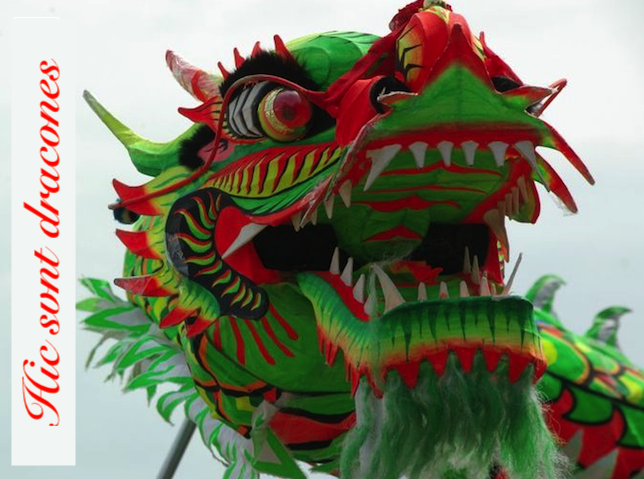
\includegraphics[width=0.75\textwidth]{imagenes/hic-svnt-dracones}
	\vspace{2cm}
	\begin{flushright}
		{\normalsize \textcolor{darkgray}{\textit{Ignacio Vallés Oriola}} \par}
	\end{flushright}
\end{titlepage}


\tableofcontents

\chapter*{}

\vspace{-4cm}

\textsf{Este libro está enfocado a aquellos alumnos que van a emprender carreras científicas que necesitan de más contenidos matemáticos que los aprendidos en bachillerato, por tanto, se suponen conocidos todos los temas allí tratados, quien lea el libro debe saber manejarse con soltura ante sistemas de ecuaciones lineales, matrices y determinantes, conocer el producto escalar y vectorial de vectores y saber derivar e integrar con soltura.} 

\textsf{Se mostrarán, de forma sencilla y con ejercicios resueltos (y propuestos con solución) algunos de los temas que se afrontarán en los primeros cursos de carrera. Para ello es necesario perder el rigor necesario en matemáticas pero será en pos de aclarar los conceptos, al cursar estudios universitarios se recuperará el rigor que ahora, de momento, abandonamos. Espero que sea de utilidad.}

\textsf{He incluidos los temas que figuran en el índice y considero este trabaja abierto a posibles modificaciones e inclusión de otros temas de interés.}


\vspace{1cm}

\textbf{Estructura}

No he sido demasiado exigente a la hora de usar el mismo formato en todos los textos, pero aparecerán:

\begin{cuadro-gris}
	
\end{cuadro-gris}

\begin{cuadro-naranja}
	
\end{cuadro-naranja}

\begin{destacado}
	
\end{destacado}

\begin{miejercicio}
	
\end{miejercicio}

\begin{mipropuesto}
	
\end{mipropuesto}

\begin{theorem}
	
\end{theorem}

\begin{definition}
	
\end{definition}







\begin{comment}

%%%%%%%%%%%%%%%%%%%%%%%%%%%%%%%%%%%. SECCIONES
\chapter{texto}
\begin{tikzpicture}
	\fill [left color=red!50, right color=teal!50] (0,0) rectangle (6.5,.2);
	\fill [left color=teal!50, right color=blue!50] (6.5,0) rectangle (11.5,.2);
	\end{tikzpicture}

\vspace{1cm}
\section{texto}
\begin{tikzpicture}
	\fill [left color=red!50, right color=teal!50] (0,0) rectangle (3.5,.1);
	\fill [left color=teal!50, right color=blue!50] (3.5,0) rectangle (7.5,.1);
	\end{tikzpicture}
\vspace{0.5cm}

\subsection{texto}
\begin{tikzpicture}
	\fill [left color=red!50, right color=teal!50] (0,0) rectangle (3.5,.01);
	\fill [left color=teal!50, right color=blue!50] (3.5,0) rectangle (7.5,.01);
	\end{tikzpicture}
\vspace{0.5cm}


%%%%%%%%%%%%%%%%%%%%%%%%%%%%%%%%%%%. \begin{ ------>. 
detsacado;  cuadro-naranja;  cuadro-gris;  miejercicio (solución extensa);  mipropuesto (solución corta y fuera del cuadro)

%%%%%%%%%%%%%%%%%%%%%%%%%%%%%%%%%%%. CURIOSIDAD
\vspace{1cm}
\color{ForestGreen!80}
\rule{250pt}{0.2pt}
Texto
\vspace{-8mm}
\begin{flushright}
\rule{250pt}{0.2pt}		
\end{flushright}	
\color{black}
\end{comment}



\emph{\normalsize{Este} documento se comparte bajo licencia `Creative Commons Attribution-NonCommercial-ShareAlike (4.0 CC BY-NC-SA)'}


\begin{multicols}{2}
\begin{figure}[H]
	\centering
	
\includegraphics[width=.5
	\textwidth]{imagenes/licencia.png}
	
\end{figure}
\begin{figure}[H]
	\centering
	
\includegraphics[width=.25
	\textwidth]{imagenes/firma.png}
\end{figure}
\end{multicols}

\newpage




\newpage

$\,$

\newpage

$\,$

\vspace{1cm} 

$\,$

\begin{figure}[H]
	\centering
	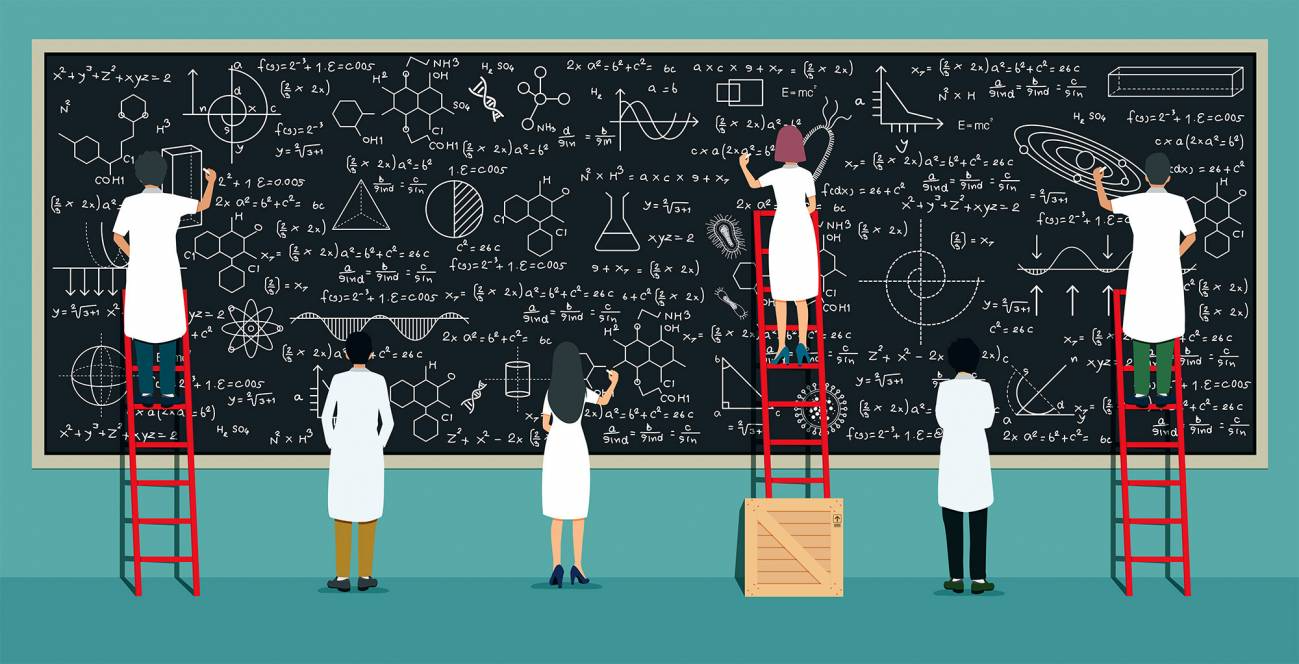
\includegraphics[width=.80\textwidth]{imagenes/presenta1.png}
\end{figure}


\begin{center}

\Huge{\textbf{Ampliación de Matemáticas:}}

\huge{\textbf{del Instituto a la Facultad}} 


\Large{\textbf{\textit{Una visión introductoria}}}

\vspace{10mm}
\begin{figure}[H]
	\centering
	
\includegraphics[width=.78\textwidth]{imagenes/presenta2.png}
\end{figure}

\vspace{2cm}
\begin{flushright}
	\normalsize{\emph{Ignacio Vallés Oriola}}
\end{flushright}


\end{center}






%\chapter{Conceptos básicos}
\setlength{\parindent}{0cm}

\begin{tikzpicture}
	\fill [left color=red!50, right color=teal!50] (0,0) rectangle (6.5,.2);
	\fill [left color=teal!50, right color=blue!50] (6.5,0) rectangle (11.5,.2);
	\end{tikzpicture}
\begin{comment}
\vspace{1cm}
\section{Uno.Uno}
\begin{tikzpicture}
	\fill [left color=red!50, right color=teal!50] (0,0) rectangle (3.5,.1);
	\fill [left color=teal!50, right color=blue!50] (3.5,0) rectangle (7.5,.1);
	\end{tikzpicture}
\vspace{0.5cm}

\vspace{1cm}
\subsection{Uno.Uno.Uno}
\begin{tikzpicture}
	\fill [left color=red!50, right color=teal!50] (0,0) rectangle (3.5,.01);
	\fill [left color=teal!50, right color=blue!50] (3.5,0) rectangle (7.5,.01);
	\end{tikzpicture}
\vspace{0.5cm}

\end{comment}\vspace{1cm}
\section{Sección}

\begin{tikzpicture}
	\fill [left color=red!50, right color=teal!50] (0,0) rectangle (3.5,.1);
	\fill [left color=teal!50, right color=blue!50] (3.5,0) rectangle (7.5,.1);
\end{tikzpicture}


chsal<ka ahD JHA DHAhd ahDJHAhdjahdjh ajhjkdhaD JAHJKDAJSHDJKHAS DHJAKSHDJK SAHJASHXJKHJKhjkhjkhjkhchajkc hkjK.N KJC SD K Kk h. s hsah hsjlk chsdj cjskd cjsdh jklds 

chsal<ka ahD JHA DHAhd ahDJHAhdjahdjh ajhjkdhaD JAHJKDAJSHDJKHAS DHJAKSHDJK SAHJASHXJKHJKhjkhjkhjkhchajkc hkjK.N KJC SD K Kk h. s hsah hsjlk chsdj cjskd cjsdh jklds 

chsal<ka ahD JHA DHAhd ahDJHAhdjahdjh ajhjkdhaD JAHJKDAJSHDJKHAS DHJAKSHDJK SAHJASHXJKHJKhjkhjkhjkhchajkc hkjK.N KJC SD K Kk h. s hsah hsjlk chsdj cjskd cjsdh jklds  %conceptos básicos
\chapter{Derivadas en física}
\begin{tikzpicture}
	\fill [left color=red!50, right color=teal!50] (0,0) rectangle (6.5,.2);
	\fill [left color=teal!50, right color=blue!50] (6.5,0) rectangle (11.5,.2);
	\end{tikzpicture}


\begin{comment}
\vspace{1cm}
\section{Uno.Uno}
\begin{tikzpicture}
	\fill [left color=red!50, right color=teal!50] (0,0) rectangle (3.5,.1);
	\fill [left color=teal!50, right color=blue!50] (3.5,0) rectangle (7.5,.1);
	\end{tikzpicture}
\vspace{0.5cm}

\vspace{1cm}
\subsection{Uno.Uno.Uno}
\begin{tikzpicture}
	\fill [left color=red!50, right color=teal!50] (0,0) rectangle (3.5,.01);
	\fill [left color=teal!50, right color=blue!50] (3.5,0) rectangle (7.5,.01);
	\end{tikzpicture}
\vspace{0.5cm}

\end{comment}


\vspace{1cm}
\section{La diferencial en física}
\begin{tikzpicture}
	\fill [left color=red!50, right color=teal!50] (0,0) rectangle (3.5,.1);
	\fill [left color=teal!50, right color=blue!50] (3.5,0) rectangle (7.5,.1);
	\end{tikzpicture}
\vspace{0.5cm}

\setlength{\parindent}{0cm}

\begin{destacado}
\emph{``Un \textbf{diferencial} de una magnitud es una cantidad muy pequeña (infinitesimal) de dicha magnitud.''} 
\end{destacado}

Pero, ?`cómo de pequeña ha de ser la cantidad para considerarla un \emph{diferencial}?\footnote{Diferencial, infinitesimal o infinitésimo, frente a infinito, son números (hiperreales) que, sin ser cero, son menores  en valor absoluto que cualquier número real positivo. $\quad$ Matemáticamente, $\ \ A \text { infinitesimal si }\displaystyle \lim_{t\to 0}{A(t)}=0$ } Pues depende, el concepto diferencial ha de ser siempre en relación a los valores típicos que presente la variable en el campo de estudio. Por ejemplo, la cantidad de $1$ metro, en el sistema de estudio del movimiento de la tierra alrededor del sol sí puede ser considerada una cantidad diferencial pero no si el sistema en estudio son los sucesivos rebotes de una pelota dejada caer desde una mesa.

Si tenemos una magnitud que es función de varias variables, $f(x,y,\cdots)$, y estas sufren pequeños cambios diferenciales $x\to x+\dd x,\ y\to y+\dd y,\cdots $ entones, el cambio de nuestra magnitud será:
$\dd f=f(x+\dd x ,y+\dd y, \cdots) - f(x,y,\cdots)$


$\centerdot\ \ $ Si nuestra función es suma (resta) de otras dos,

$\qquad f=u+v  \ \to \ \left\{ 
\begin{matrix}  \ u\to u+\dd u \\ \ v\to v+\dd v  \end{matrix} 
\right. \quad \Rightarrow \ \boldsymbol{\dd f} = (u+\dd u)+(v+\dd v)- (u+ v)= \boldsymbol{ \dd u + \dd v }$	

$\centerdot \ \ $ Si nuestra función es producto de otras dos,

$\qquad f=u\, v  \ \to \ \left\{ 
\begin{matrix}  \ u\to u+\dd u \\ \ v\to v+\dd v  \end{matrix} 
\right. \quad \Rightarrow \ \boldsymbol{\dd f} = (u+\dd u)\ (v+\dd v)- (u\,v)= $

$\qquad =\cancel{u\, v} + u\dd v +v\dd u +\cancelto{0\ (*)}{ \dd u\, \dd v } - \cancel{u\, v}= \boldsymbol{ u\dd v +v\dd u}$	

\textcolor{gris}{
$(*) \qquad $ Si, por ejemplo, $\dd u \sim 10^{-3}$ y $\dd v \sim 10^{-3} \ \to \ \dd u\, \dd v  \sim 10^{-6}$, despreciable frente a los anteriores, se le llama diferencial de orden dos.}

Cuando el resultado de una operación sea suma de varios diferenciales, en primera aproximación, los diferenciales de orden superior al primero son despreciables frente a estos (producto de dos diferenciales es un diferencial de orden dos, el producto de tres de ellos es un diferencial de orden tres, etc.)

\emph{Dimensionalmente}, un diferencial tiene las mismas unidades de la magnitud de la que proviene.



\vspace{1cm}
\section{La derivada en física}
\begin{tikzpicture}
	\fill [left color=red!50, right color=teal!50] (0,0) rectangle (3.5,.1);
	\fill [left color=teal!50, right color=blue!50] (3.5,0) rectangle (7.5,.1);
	\end{tikzpicture}
\vspace{0.5cm}

\subrayado{\emph{``Una \textbf{derivada} en física es un cociente entre dos diferenciales (cantidades muy pequeñas'')}.}

\begin{figure}[H]
	\centering
	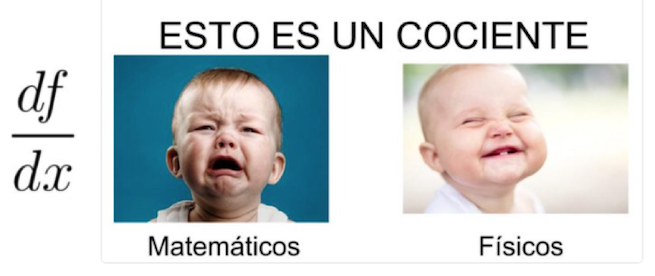
\includegraphics[width=.6\textwidth]{imagenes/T02IM01.png}
\end{figure}


Muchas leyes de la Física, la Química, la Biología o la Economía, son funciones que relacionan una variable `dependiente' y con otra variable `independiente' $x$, lo que suele escribirse en la forma $y = f(x)$. Si la variable independiente cambia de un valor inicial $x_0$ a otro $x$, la variable y lo hace de $f(x_0)$ a $f(x)$. La razón de cambio promedio o `tasa de variación media' de $y = f(x)$ con respecto a $x$ en el intervalo $[x_0,x]$ es: $\dfrac{\Delta f}{\Delta x}=\dfrac{f(x)-f(x_0)}{x-x_0}$

Con frecuencia interesa considerar la razón de cambio en intervalos cada vez más pequeños. Esto lleva a definir lo que podemos llamar `razón de cambio instantáneo' o `tasa de variación instantánea' de $y = f(x)$ con respecto a $x$ en el punto $x_0$ como: 
$\displaystyle \lim_{x\to x_0} \dfrac{f(x)-f(x_0)}{x-x_0} =\dfrac {\dd f}{\dd x}=f'(x)$

Un ejemplo clásico es la velocidad instantánea $v(t)$ en contraposición a la velocidad media $\bar v = \dfrac{\Delta x}{\Delta t}$, definida como:
$\quad  \displaystyle \boldsymbol{ v(t)= \dv{x}{t} } \ =\lim_{\Delta t\to 0} \dfrac{\Delta x}{\Delta t}$

En matemáticas, $\quad f(u)\ \to \ \displaystyle \dv{f}{u}=\dfrac{f(u+\dd u)-f(u)}{\dd u}= \ \mqty [ \dd u = h \\ h \to 0] \ = \lim_{h\to 0} \dfrac {f(u+h)-f(u)}{h}=f'(u)\ . \  \ $ Geométricamente coincide con la pendiente de la recta tangente a la función en el punto en que se calcule.

En física se suele usar la notación de Leibniz, $\displaystyle \dv{f}{u}$ preferiblemente a la de Lagrange $f'(u)$. \textcolor{gris}{Aún se usa otra notación en física, cuando la variable sobre la que se deriva es el tiempo $t$ es frecuente usar la notación de Newton $\dot f(t)=\displaystyle \dv{f}{t}=f'(t)$}

En la notación de Leibniz, tan importante es la magnitud a derivar como aquella respecto de la cual se deriva. $\displaystyle \ \dv{f}{u}\ $ se lee como \emph{derivada de $f$ respecto de $u$}.

\vspace{3mm} Puesto que $\qquad \qquad \displaystyle \subrayado{\ \boxed{\ \boldsymbol{ \dv{f}{u}=f'(u)} \ } \ } \qquad \to \qquad \subrayado{\  \boxed{ \ \boldsymbol{ \dd f \ = \ f'(u)\, \dd u } \ } \ }\ ,$

que pone de manifiesto la \emph{\textbf{relación entre derivada y diferencial.}}

\vspace{3mm} \textcolor{gris}{Al igual que un diferencial no siempre es la variación de una variable, p.e. $\dd V=\dd x\, \dd y\, \dd z$ es el producto de tres diferenciales de variables distintas, del mismo modo  no siempre un cociente de diferenciales será una derivada, $\rho=\dd m/\dd V$, la densidad no es la derivada de la masa respecto del volumen. Si la densidad no es constante, un pequeño elemento de volumen $\dd V$ tendrá una pequeña masa $\dd m$ que determinarán su densidad  $\rho=\dd m/\dd v$.}

\vspace{3mm} Dimensionalmente, al ser la derivada un cociente entre diferenciales, las unidades de la derivada son el cociente entre las unidades del \emph{numerador} y las del \emph{denominador}: 

$\quad \displaystyle \left[ \dv{f}{u} \right]=\dfrac{[f]}{[u]};
 \qquad [v]=\dfrac{[\dd x]}{[\dd t]}=\dfrac {\mathrm{m}}{\mathrm{s}}=\mathrm{m\, s}^{-1}$ 


\vspace{1cm}
\subsection{Álgebra de derivadas}
\begin{tikzpicture}
	\fill [left color=red!50, right color=teal!50] (0,0) rectangle (3.5,.01);
	\fill [left color=teal!50, right color=blue!50] (3.5,0) rectangle (7.5,.01);
	\end{tikzpicture}
\vspace{0.5cm}


\ul{Suma y producto}: 

$\quad \displaystyle \dv{(u+v)}{t}=\dfrac{\dd u + \dd v}{\dd t}=\dv{u}{t}+\dv{v}{t}$
$\qquad \qquad $
$\displaystyle \dv{(u\, v)}{t}=\dfrac{\dd u \, v+ u\, \dd v}{\dd t}=\dv{u}{t}\, v+ u\, \dv{v}{t}$

\vspace{5mm} Para \ul{magnitudes vectoriales}: 

$\quad	\overrightarrow A=A_x\vec i+A_y\vec j+A_z\vec k \quad \to \quad \displaystyle \dv{\overrightarrow A}{t}=\dv{A_x}{t}\vec i+\dv{A_y}{t}\vec j+\dv{A_z}{t}\vec k $


$\quad \displaystyle \dv{(\lambda \overrightarrow A)}{t}=\dv{\lambda}{t}\overrightarrow A+\lambda \dv{\overrightarrow A}{t};$

$\quad  \displaystyle  \dv{t} (\overrightarrow A \cdot \overrightarrow B)= \dv{\overrightarrow A}{t} \cdot \overrightarrow B + \overrightarrow A \cdot \dv{\overrightarrow B}{t}; \qquad \dv{t} (\overrightarrow A \times \overrightarrow B)= \dv{\overrightarrow A}{t} \times \overrightarrow B + \overrightarrow A \times \dv{\overrightarrow B}{t}$

\vspace{2mm} \textcolor{gris}{$\quad \overrightarrow A \cdot \overrightarrow  B \text{ producto escalar,} \quad \overrightarrow A \times \overrightarrow  B \text{ producto vectorial}$}

\vspace{5mm} Función compuesta, \ul{regla de la cadena}:

$A(x),\ x(t) \quad \to \qquad \displaystyle \dv{A}{t}=\dv{A}{x}\, \dv{x}{t}$
$\qquad \qquad \qquad $
$A(u),\, u(x),\,  x(t) \quad \to \qquad \displaystyle \dv{A}{t}=\dv{A}{u}\,  \dv{u}{x}\, \dv{x}{t}$

\vspace{5mm} Derivada de la \underline{función inversa}:

En notación de Lagrange: $\ 	\displaystyle \left( f^{-1} \right)\, ' \ = \ \dfrac 1{f'(f^{-1}(x))}\, ; \ \ $ en notación de Leibniz: $\ \ \displaystyle \dv{y}{x} \ = \ \dfrac{1}{\displaystyle \dv{x}{y}}$

\vspace{5mm} \ul{Derivadas de orden superior}:
$\quad \displaystyle \dv{t}\, \dv{A}{t}= \dv[2]{A}{t}=A''(t)=\ddot A(t) \ ; \qquad \  \dv{t}\, \dv[2]{A}{t}=\dv[3]{A}{t}\, ; \qquad \dv[n]{A}{t} $

Se leen, respectivamente, `derivada segunda de $A$ respecto de $t$ dos veces, derivada tercera de $A$ respecto de $t$ tres veces, derivada enésima de $A$ respecto de $t$ $n$ veces'.

No confundir $\quad \displaystyle \dv[2]{A}{t} \neq \left( \dv{A}{t} \right)^2\, , \ $ son incluso dimensionalmente cosas distintas: 

\textcolor{gris}{$\displaystyle \left[ \dv[2]{A}{t}  \right]=\dfrac{[A]}{[t^2]} \ \neq \ \dfrac{[A^2]}{[t^2]} = \left[ \left( \dv{A}{t} \right)^2 \right]\quad $ Por ejemplo, $\ \displaystyle a=\dv{v}{t}=\dv{t} \left( \dv{x}{t} \right) = \dv[2]{x}{t} \ \to \ \dfrac {\mathrm{m}}{\mathrm{s}^2} \ \ \bcancel{\cancel{ \dfrac {\mathrm{m}^2}{\mathrm{s}^2} }}$}

\vspace{1cm}
\color{ForestGreen!80}
\rule{250pt}{0.2pt}


\textsf{Leibniz fue quién mejor comprendió la importancia de una buena elección de los símbolos a usar en matemáticas, una vez introducida una notación la experimentaba durante mucho tiempo e incluso mantenía discusiones al respecto con sus colegas.}

\textsf{Leibniz, al límite del cociente incremental de una función en un punto (derivada), $\displaystyle \lim_{\Delta x \to 0} {\Delta f}/{\Delta x}$ le llamaba cociente de de diferenciales $\displaystyle \dd f  / \dd x$.}

\textsf{No solo era distinta la notación sino la forma de pensar. Leibniz pensaba, en lugar de límite de cantidades incrementales, que la derivada se obtenía cuando se pasaba de estas a cantidades incrementales a las cantidades \emph{diferenciales} siendo la \emph{derivada un cociente diferencial}, los incrementos $\Delta x,\, \Delta y$, al calcular la derivada se transformaban en \emph{infinitesinales} $\dd x,\, \dd y$, un \emph{nuevo tipo de números reales, que sin ser cero, son más pequeños en valor absoluto que cualquier número real positivo}.}

\textsf{Cauchy (s.XIX) abandonó el concepto de infinitesimales aunque se siguen usando en matemáticas aplicadas. La notación de Leibniz tiene la ventaja  de simplificar las operaciones y sus fórmulas se recuerdan sin dificultad.}

\vspace{-8mm}
\begin{flushright}
\rule{250pt}{0.2pt}		
\end{flushright}

	
\color{black}





\vspace{1cm}
\section{Derivadas parciales}
\begin{tikzpicture}
	\fill [left color=red!50, right color=teal!50] (0,0) rectangle (3.5,.1);
	\fill [left color=teal!50, right color=blue!50] (3.5,0) rectangle (7.5,.1);
	\end{tikzpicture}
\vspace{0.5cm}

Es muy frecuente que al estudiar determinadas magnitudes éstas dependan de varias variables: \emph{funciones de varias variables}.
\emph{ {La \textbf{derivada parcial} de una función $f(x,y,\cdots)$ respecto de una de ellas, p.e. la $x$, se obtiene derivando la expresión de $f$ respecto de  $x$ de modo usual solo que considerando que el resto de las variables son constantes}.} 
Se denota por $\displaystyle \pdv{f}{x}$ y se lee \emph{derivada parcial de $f$ respecto de $x$}.


Así, se habla de $\quad f(x,y,z,\cdots )\quad \to \quad\displaystyle \pdv{f}{x},\ \pdv{f}{y},\ \pdv[2]{f}{x}{y},\ \pdv[2]{f}{x},\ $ etc.

\vspace{5mm}\textcolor{gris}{$\triangleright \quad \ \text{ si } \ f(x,y)=x^2+3xy^2+2y^3 \ \quad \to \ \quad 
\displaystyle \pdv{f}{x}=2x+3y^2,\qquad \pdv{f}{y}=6xy+6y^2,\qquad \pdv[2]{f}{x}{y}=\pdv{x} \left( \pdv{f}{y} \right)= \pdv{x} (6xy+6y^2)=6y,\qquad \pdv[2]{f}{x} =\pdv{x} \left( \pdv{f}{x} \right)= \pdv{x} (2x+3y^2)=2x  $}

\vspace{3mm}\textcolor{gris}{$\triangleright \quad \ \text{ si } \  V_{cono}(r,h)=\dfrac \pi 3  r^2 h \ \quad \to \ \quad 
\displaystyle \pdv{V}{r}=\dfrac{2\pi}{3}rh;\quad\pdv{V}{h}=\dfrac \pi 3 r^2$}


\vspace{5mm}  Sea $f(x_1,x_2, \cdots , x_n)\ \ $
Se define la \emph{derivada total} resprecto a una de las variables como:

$$\displaystyle \boxed{\ \subrayado{\  \boldsymbol{ \dv{f}{x_i}=\pdv{f}{x_1}\dv{x_1}{x_i} + \pdv{f}{x_2}\dv{x_2}{x_i} + \cdots \pdv{f}{x_{i-1}}\dv{x_{i-1}}{x_i} + \pdv{f}{xi} + \pdv{f}{x_{i+1}}\dv{x_{i+1}}{x_i} + \cdots + \pdv{f}{x_n}\dv{x_n}{x_i} } \ } \ }$$

\vspace{3mm} y la \emph{diferencial} de una función de varias variables como:

\begin{small}$$ \boxed{\ \subrayado{\ \boldsymbol{ \displaystyle \dd f= \pdv{f}{x_1}\dd x_1 + \pdv{f}{x_2}\dd x_2 + \cdots + \pdv{f}{x_i}\dd x_i + \cdots +\pdv{f}{x_n}\dd x_n }  \ } \ }$$\end{small}

\vspace{5mm} \textcolor{gris}{\normalsize{Siguiendo} con los ejemplos anteriores,}

\vspace{3mm}\textcolor{gris}{$\triangleright \quad \displaystyle \dv{f}{x}=\pdv{f}{x}+\pdv{f}{y} \, \dv{y}{x}=2x+3y^3+(6xy+6y^2)\, \dv{y}{x} $}

\vspace{3mm}\textcolor{gris}{$\triangleright \quad \displaystyle \dd V= \pdv{V}{r}\, \dd r + \pdv{V}{h} \, \dd h=\dfrac{2\pi}3 rh \, \dd r + \dfrac \pi 3 r^2 \, \dd h  $}

\vspace{3mm}\textcolor{gris}{$\triangleright \quad \displaystyle \dv{V}{r}=\pdv{V}{r}+\pdv{V}{h}\, \dv{h}{r};\qquad  \dv{V}{h}=\pdv{V}{r}\, \dv{r}{h}+\pdv{V}{h};$}

\vspace{1mm}\textcolor{gris}{$\displaystyle \text{si } r=r(t) \ \wedge \ h=h(t) \ \to \  \dv{V}{t}=\pdv{V}{r} \, \dv{r}{t}+\pdv{V}{h} \, \dv{h}{t}$}

\vspace{5mm} \textbf{Derivadas parciales de orden superior}

Se definen:

$\displaystyle \pdv[2]{f}{x}=\pdv{x} \left( \pdv{f}{x} \right);\qquad  \pdv[2]{f}{x}{y}=\pdv{x} \left( \pdv{f}{y} \right);\qquad $ en general, $\quad \displaystyle \pdv[n]{f}{x} =\pdv{x} \left( \pdv[n-1]{f}{x} \right)$


\begin{cuadro-naranja}
	
\textbf{Teorema de Clairaut (o de Schwartz)}:

``Si las derivadas parciales cruzadas existen y son continuas, entonces coinciden'' 

$$\quad \displaystyle \boldsymbol{\pdv[2]{f}{x}{y}=\pdv[2]{f}{y}{x}}$$
\end{cuadro-naranja}

\vspace{2mm}\textcolor{gris}{En el ejemplo anterior, $ \displaystyle f(x,y)=x^2+3xy^2+2y^3 \ \quad \to \ \quad 
\displaystyle \pdv{f}{x}=2x+3y^2,\quad \pdv{f}{y}=6xy+6y^2 $}

\vspace{2mm}\textcolor{gris}{$\displaystyle \pdv[2]{f}{x}{y}=\pdv{x} \left( \pdv{f}{y} \right) = \pdv{x}(6xy+6y^2)=6y \ \boldsymbol{=} \ \pdv[2]{f}{y}{x}=\pdv{y} \left( \pdv{f}{x} \right) = \pdv{y} (2x+3y^2)=6y  $} 


\vspace{5mm} Otra notación para las derivadas parciales: $\quad \displaystyle \pdv{f}{x}=f_x;\quad \pdv[2]{f}{x}{y}=f_{xy};\quad \pdv[2]{f}{x}=f_{xx}$



\vspace{1cm}
\section{Ejercicios}
\begin{tikzpicture}
	\fill [left color=red!50, right color=teal!50] (0,0) rectangle (3.5,.1);
	\fill [left color=teal!50, right color=blue!50] (3.5,0) rectangle (7.5,.1);
	\end{tikzpicture}
\vspace{0.5cm}


\vspace{1cm}
\begin{miejercicio}
		\textsf{La posición de una partícula viene dada por la expresión $x(t)=(2t+3t^2)\, \mathrm{m}$	 con $t(\mathrm{s})$. Determinar la velocidad media en el intervalo $[0,3]\, \mathrm{s}$ así como la velocidad  y la aceleración instantáneas a los $3\, \mathrm{s}$.}


\color{teal!80}
\rule{200pt}{0.2pt}

\vspace{5mm}
\color{black}

$\displaystyle \bar v=\dfrac{\Delta x}{\Delta t};\qquad v=\dv{x}{t};\qquad a=\dv[2]{x}{t}=\dv{v}{t} $

\vspace{2mm}$v(0)=0\, ;\quad v(3)=2\cdot 3+3\cdot t^2=33 \quad \to \qquad \bar v=\dfrac{v(3)-v(0)}{3-0}=\dfrac {33}3=11\, \mathrm{m\, s}^{-1}$

\vspace{2mm}$v(t)=\displaystyle \dv{x}{t}=2+6t \quad \to \qquad v(3)=2+6\cdot 3=20 \,  \mathrm{m\, s}^{-1}$

\vspace{2mm}$a(t)=\displaystyle \dv{v}{t}=6 \quad \to \qquad a(3)=6\,  \mathrm{m}\,\mathrm{s}^{-2}$

\end{miejercicio}

\vspace{1cm}
\begin{miejercicio}
.	Sean $\quad \overrightarrow A(t)=3t\vec i-t^2\vec j;\ \ \overrightarrow B(t)=\vec i-2t\vec j+e^t\vec k$. 

\vspace{3mm} Comprobar que $\quad \displaystyle \dv{t} (\overrightarrow A \cdot \overrightarrow B)= \dv{\overrightarrow A}{t} \cdot \overrightarrow B + \overrightarrow A \cdot \dv{\overrightarrow B}{t}$

\color{teal!80}
\rule{200pt}{0.2pt}
\color{black}
\vspace{5mm}

 $\overrightarrow A(t)=3t\vec i-t^2\vec j;\ \ \overrightarrow B(t)=\vec i-2t\vec j+e^t\vec k \qquad \displaystyle \dv{\overrightarrow A}{t}=3\vec i-2t\vec j; \ \ \dv{\overrightarrow B}{t}=-2\vec j+e^t\vec k$ 	
 
 $\overrightarrow A \cdot \overrightarrow B=(3t\vec i-t^2\vec j)\cdot(\vec i-2t\vec j+e^t\vec k)=3t+2t^3 \quad \to \quad \displaystyle \dv{\overrightarrow A \cdot \overrightarrow B}{t}=3+6t2 \ \checkmark$
 
 $\displaystyle \dv{\overrightarrow A}{t} \cdot \overrightarrow B + \overrightarrow A \cdot \dv{\overrightarrow B}{t} = (3\vec i -2t \vec j)\cdot(\vec i-2t\vec j+e^t\vec k)+(3t\vec i-t^2\vec j)\cdot((-2\vec j+e^t\vec k)=(3+4t^2)+2t^2=3+6t^2 \ \checkmark$

\end{miejercicio}


\vspace{1cm}
\begin{miejercicio}
.	a) Sea $\ z=\cos y;\ \ y=\ln(x+1);\ \ x=3t^2+5\ $ Calcular $\displaystyle \dv{z}{t}=\dot z$

	b) Sea $\ y=\mathrm{arc} \, \mathrm{csc} \ x\ $ Calcula $\displaystyle \dv{y}{x}$

\color{teal!80}
\rule{200pt}{0.2pt}
\color{black}
\vspace{5mm}
	
	$a)\qquad \displaystyle \dot z=\dv{z}{t}=\dv{z}{y}\, \dv{y}{x}\, \dv{x}{t}= -\sin y\, \dfrac 1{x+1}\, 6t = -\sin(\, \ln(3t^2+6)\, ) \, \dfrac{1}{3t^2+6}\, 6t$
	
\vspace{3mm} $b)\quad \displaystyle y=\mathrm{arc} \, \mathrm{csc} \ x  \leftrightarrow  x=\mathrm{csc}\, y=\dfrac 1{\cos y} \quad \textcolor{gris}{\left( \cos y=\dfrac 1 x \right) } \ \  \to \ \  \dv{x}{y}=-\dfrac{1}{\cos^2 y}\, \sin y \quad$ 
	
\vspace{3mm}  $\displaystyle \dv{y}{x}=\dfrac{1}{\displaystyle \dv{x}{y}}=-\dfrac{\cos^2 y}{\sin y}=-\dfrac{\cos^2}{\sqrt{1-\cos^2 x}}=-\dfrac {(1/x)^2}{\sqrt{1-(1/x)^2}}=-\dfrac{1}{x\sqrt{x^2-1}} \quad$ 

\end{miejercicio}

\vspace{1cm}
\begin{miejercicio}
.	Calcular las derivadas parciales de primer y segundo orden de la siguiente función. 
Calcular también $\ \ \displaystyle \dfrac{\partial^3 f}{\partial x \, \partial y \, \partial z}$	

$$\ f(x,y,x)=\dfrac{xy}{z}-2e^{y^2}+z^3\ln y$$

\color{teal!80}
\rule{200pt}{0.2pt}
\color{black}
\vspace{5mm}

$\displaystyle \pdv{f}{x}=\dfrac y z \, ; \qquad \pdv{f}{y}=\frac x z -4ye^{y^2} + \dfrac{z^3}{y}\, ; \qquad\pdv{f}{z}=-\dfrac{xy}{z^2}+3z^2\ln y$

\vspace{3mm} $\displaystyle \pdv[2]{f}{x}=0 \, ; \qquad \pdv[2]{f}{y}= -8y^2e^{y^2} - \dfrac{z^3}{y^2}\, ; \qquad\pdv[2]{f}{z}=-2\dfrac{xy}{z^3}+6z\ln y$

\vspace{3mm} $\displaystyle \pdv[2]{f}{x}{y}=\pdv{x}\left( \pdv{f}{y} \right) = \pdv{x}\left( \frac x z -4ye^{y^2} + \dfrac{z^3}{y} \right) = \dfrac 1 z = \pdv[2]{f}{y}{x} \qquad$ \textcolor{gris}{(Teorema de Clairaut)} 

\vspace{3mm} Del mismo modo se obtiene $\displaystyle \pdv[2]{f}{x}{z}=-\dfrac y{z^2} \quad $ y $\quad \displaystyle \pdv[2]{f}{y}{z}=-\dfrac x{z^2}+\dfrac{3x^2}y$

\vspace{3mm} \begin{small}$\displaystyle \dfrac{\partial^3 f}{\partial x \, \partial y \, \partial z}=
\pdv{x} \left( \pdv[2]{f}{y}{z} \right) =
\pdv{x} \left[ \pdv{y} \left(  \pdv{f}{z} \right) \right]=
\pdv{x} \left[ \pdv{y} \left(  -\dfrac{xy}{z^2}+3z^2\ln y \right) \right]=
\pdv{x} \left[ -\dfrac{x}{z^2}+\dfrac{3z^2}{y} \right]=-\dfrac 1{z^2}$\end{small}	

\end{miejercicio}


\vspace{1cm}
\begin{miejercicio}

Las dimensiones de un cilindro son $5$ dm de altura y $2$ dm de radio. Calcula un valor aproximado de la variación que experimenta el volumen del cilindro si, manteniéndose constante la altura, el radio aumente en un $3\, \%$


\color{teal!80}
\rule{200pt}{0.2pt}
\color{black}
\vspace{5mm}

El volumen del cilindro viene dado por la expresión $\ V = \pi r^2\, h\, .\ $ Si suponemos que la $h$ se mantiene constante, tenemos $V (r) = \pi r^2 h$. Al pasar el radio del valor $r = 2$ dm al valor $r+\dd r = 2+0.03 \cdot 2 = 2.06$ dm, el volumen experimentará un cambio $\Delta V = V (r + \dd r) - V (r)$, pero estamos buscando una aproximación, usaremos  la diferencial:
$\quad \Delta V  \approx \dd V =\pi\, 2r\, \dd r\, h=2\pi hr\, \dd r=2\pi 5\cdot 2\cdot 0.06 \approx 3.77\, \mathrm{dm}3$

\vspace{3mm} \textcolor{gris}{El cambio exacto experimentado en el volumen es} 

\vspace{2mm} \textcolor{gris}{$\Delta V=\pi\, h\, (\, (r+\dd r)^2-r^2\, ) =\pi 5 \, (2.06^2-2^2)=3.83\, \mathrm{dm}3$}
\end{miejercicio}


\vspace{1cm}
\begin{miejercicio}
.	
\begin{multicols}{2}
	$\quad$
	
	Vaciado de un tanque.
	
	\begin{adjustwidth}{20pt}{5pt}
		?`Qué tan rápido baja el nivel de líquido en un tanque cilíndrico vertical, si lo drenamos a una razón de $3000 \; l/min$?	
	\end{adjustwidth}
	$\quad$
	
	\begin{figure}[H]
	\centering
	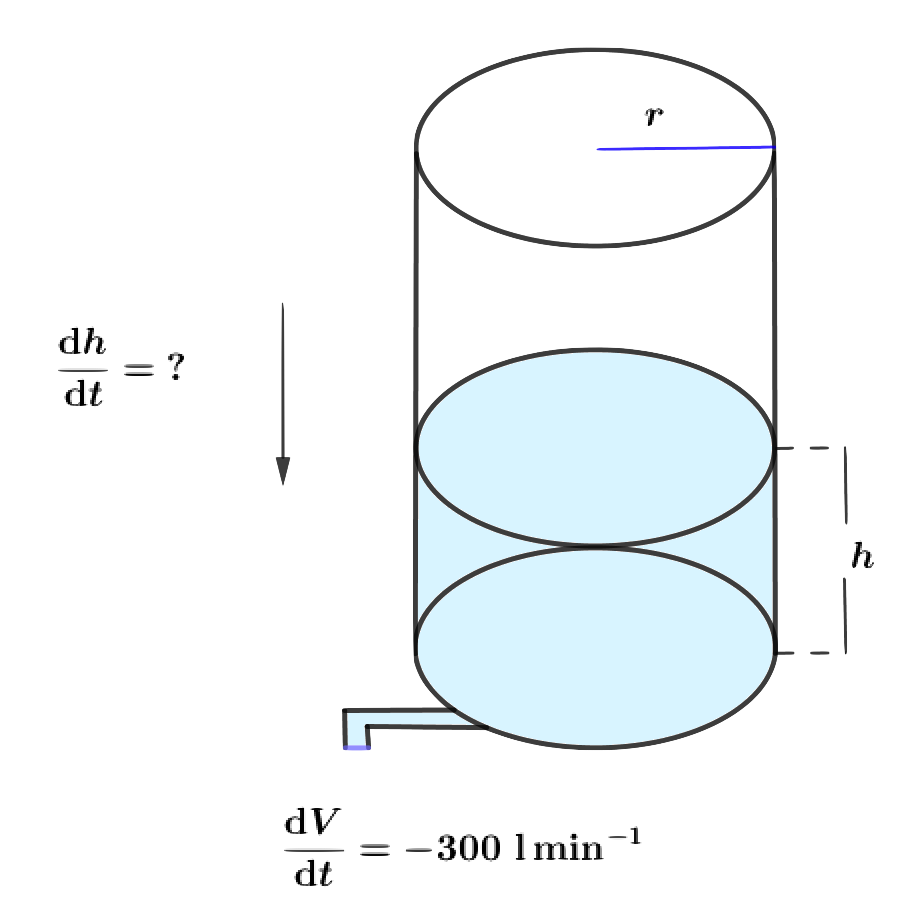
\includegraphics[width=0.35\textwidth]{imagenes/T02IM05.png}
	\end{figure}
\end{multicols}

\vspace{-10mm}
\color{teal!80}
\rule{200pt}{0.2pt}
\color{black}
\vspace{5mm}

Vamos a medir $r\,(\mathrm{m})$ y $h\,(\mathrm{m})$ con lo cual, el volumen del cilindro será $V=\pi r^2\, h \; (\mathrm{m}^3) $
	
\vspace{3mm}Vamos a resolver el problema usando la notación de Leibniz para la derivada.
	
\vspace{3mm}A medida que pasa el tiempo $t$, tendremos que tanto el volumen como la altura del líquido en el cilindro serán función de $t: \quad V(t); \; h(t)$.
	
\vspace{3mm}Derivemos la expresión 	$V(t)= \pi r^2 \; h(t)$ respecto del tiempo $t$:
	
\vspace{3mm}$\displaystyle \dv {V}{t}= \pi r^2\; \dv {h}{t}$, $\ (r$ es constante). Como $\displaystyle  \dv {V}{t}=-3000 \ \mathrm{l\, min}^{-1} \ \dfrac{1\, \mathrm{m}^3}{100 \, \mathrm{l}}= -3 \mathrm{m}^3\,\mathrm{min}^{-1} $
	
\vspace{3mm} Despejando obtenemos: $\ \ \displaystyle  \dv {h}{t}=\frac {-3}{\pi r^2}\; \mathrm{m\ min}^{-1}$.
	
\vspace{5mm}La velocidad con que baja el líquido en el tanque es constante para un radio dado y, si el radio es variable,  es inversamente proporcional al cuadrado del radio: si $r$ es grande, el líquido bajará a poca velocidad, pero si $r$ es pequeño, el líquido bajará a mayor velocidad.
	
\vspace{5mm}\textcolor{gris}{El mismo problema resuelto con notación de Lagrange sería:}
	
\vspace{3mm}\textcolor{gris}{$V(t)=\pi r^2 h(t); \quad V`(t)=-3\; \mathrm{m}^3\,\mathrm{min}^{-1} \to V'= \pi r^2 h'=-3 \ \ \to$}

\vspace{2mm}\textcolor{gris}{$\to \ \ h'(t)=-\dfrac 3 {\pi r^2}\; \mathrm{m\,min}^{-1} $}

\end{miejercicio}







\vspace{1cm}
\begin{miejercicio}

\begin{multicols}{2}
Un cilindro se comprime lateralmente y se estira, de modo que el radio de la base decrece a un ritmo de $3\,  \mathrm{cm\,s}^{-1}$ y la altura crece a $8\, \mathrm{cm\,s}^{-1}$. 

	\vspace{3mm} Hallar el ritmo al que está cambiando el volumen cuando el radio es $5\, \mathrm{cm}$ y la altura $7\, \mathrm{cm}$.	

\begin{figure}[H]
	\centering
	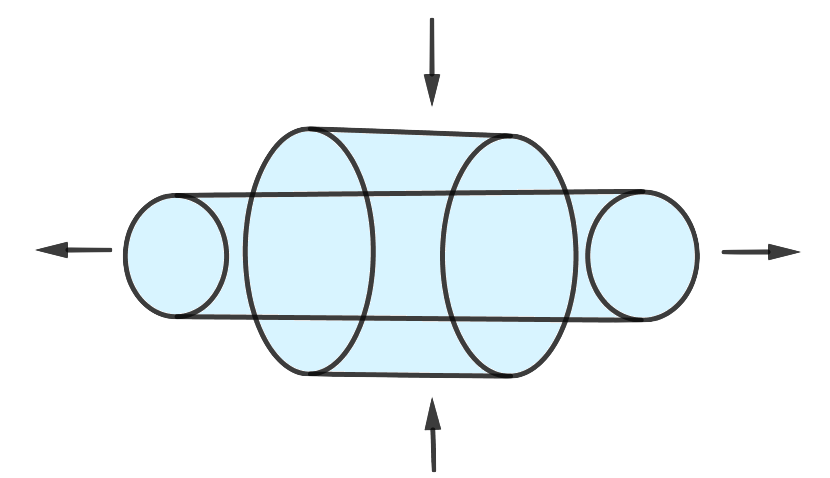
\includegraphics[width=0.4\textwidth]{imagenes/T02IM06.png}
	\end{figure}

\end{multicols}	

\vspace{-5mm}
\color{teal!80}
\rule{200pt}{0.2pt}
\color{black}
\vspace{5mm}

$\displaystyle V(r,h)=\pi r^2 h; \quad r=r(t);\ \ h=h(t)$
$\quad \to \quad $
$\displaystyle \dv{V}{t}= \pdv{V}{r}\dv{r}{t}+\pdv{V}{h}\dv{h}{t}=(2\pi rh)\, \dv{r}{t}+(\pi r^2)\, \dv{h}{t}$

\vspace{3mm} $\displaystyle \dv{r}{t}=-3\,  \mathrm{cm}\,\mathrm{s}^{-1}\, ; \qquad \dv{h}{t}=+8  \mathrm{cm}\,\mathrm{s}^{-1}$

\vspace{3mm} $\displaystyle \eval{\dv{V}{t}}_{r=5,\, h=7} = (2\pi 5\cdot 7)\, (-3) + (\pi 5^2)\, (8)=-10\pi \, \mathrm{cm^3}\,\mathrm{s}^{-1}\quad $ .

\vspace{2mm} En este momento el volumen decrece.
\end{miejercicio}




\vspace{1cm}
\begin{miejercicio}

Un depósito esférico elástico de $10$  cm  de radio	 está lleno de $He$ y se vacía a razón de $1\, \mathrm{l} \, \mathrm{min}^{-1}$. Calcular la velocidad de disminución de la superficie del depósito cuando el radio se reduce a la mitad.

\color{teal!80}
\rule{200pt}{0.2pt}
\color{black}
\vspace{5mm}

Trabajaremos las distancias en decímetros así las áreas se expresarán en dm$^2$ y los volúmenes en dm$^3=$l.

\vspace{3mm}$V_0=\dfrac 4 3 \pi r^3 =  \dfrac 4 3 \pi\,  $l.  Como se vacía a razón de $1\, \mathrm{l}\, \mathrm{min}^{-1} \ \to \ $ a los $t\, $ s la capacidad será de:

\vspace{3mm}$V(t)= \left( \dfrac 4 3 \pi - t \right) \, l \ \text{ si } t(\text{min})\ \to \  \dfrac 4 3 \pi - t = \dfrac 4 3 \pi r^3(t) \ \Rightarrow \ r(t)=\sqrt[3]{1-\dfrac 3 {4 \pi}  t}$ 

\vspace{3mm}Cuando el radio se reduce a la mitad, $0.5=\sqrt[3]{1-\dfrac 3 {4 \pi}  t} \ \to \ t=\dfrac{7\pi}{6} \,$ min.

\vspace{3mm} Como el área del depósito es $S=4\pi r^2(t)=4\pi \left( 1-\dfrac 3 {4 \pi}  t \right)^{2/3}$, y la velocidad a la que decrece el área será : $\ \displaystyle \dv{S}{t}=4\pi \dfrac 2 3 \left( 1-\dfrac 3 {4 \pi}  t \right)^{-1/3} \left( \dfrac{-3}{4\pi} \right)=-2 \left( 1-\dfrac 3 {4 \pi}  t \right)^{-1/3}$

\vspace{3mm} Cuando $r=0.5 \, \mathrm{dm} \ \to \ t=\dfrac{7\pi}{6} \, \mathrm{min} \ \Rightarrow \ \displaystyle \eval{\dv{S}{t}}_{t=\frac{7\pi}{6}}\ = \ -4 \, \mathrm{dm}^2\mathrm{min}^{-1}$

\end{miejercicio}







\vspace{1cm}
\begin{miejercicio}

\begin{multicols}{2}
	
	Un globo aerostático que asciende en línea recta desde el nivel del suelo es rastreado por un observador que está a $500\; m$  del punto de elevación. El momento en el que el ángulo de elevación es de $\pi/4$, el ángulo crece a razón de $0.14\; \mathrm{rad/min}$. ?`Qué tan rápido se está elevando el globo en ese momento? 
	\begin{figure}[H]
	\centering
	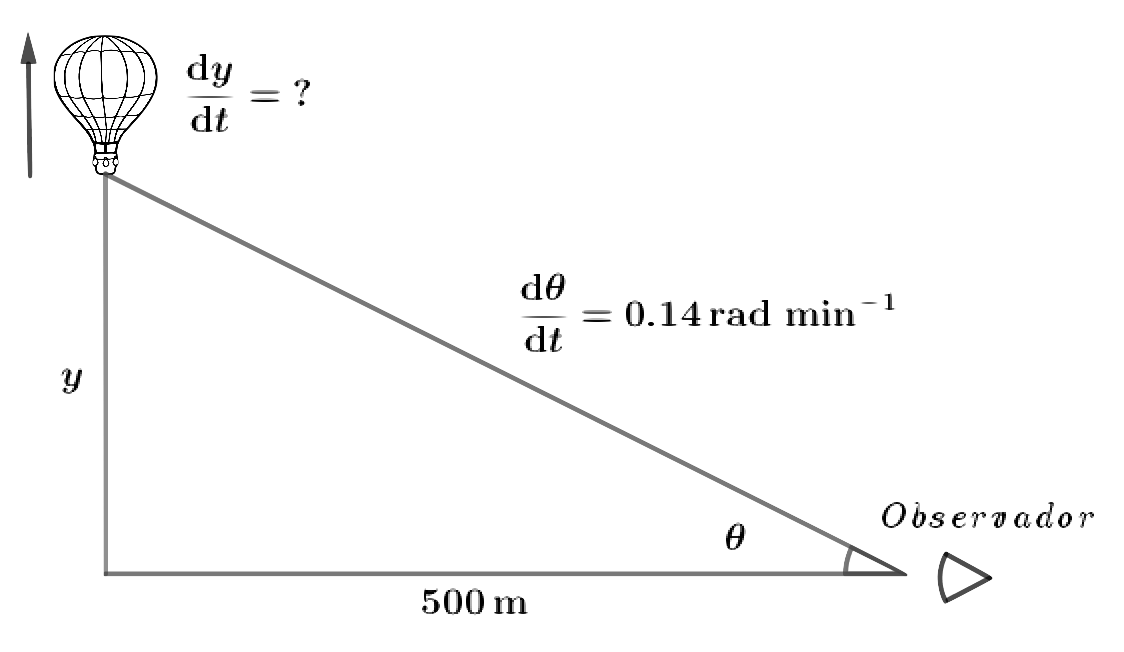
\includegraphics[width=0.5\textwidth]{imagenes/T02IM08.png}
	\end{figure}		
	\end{multicols}
\color{teal!80}
\rule{200pt}{0.2pt}
\color{black}
\vspace{5mm}

$t(\mathrm{min})\, ; \ \ \theta(t)\,; \ \ y(t)\, ; \ \ \displaystyle \dv{\theta}{t}=0.14 \, \mathrm{rad\, min}^{-1}\ ; \  \qquad \text{ Para } \ \ \theta=\pi/4 \ \Rightarrow \ \displaystyle \dv{\theta}{t}\, ?   $

\vspace{3mm} De la figura: $\quad 	\dfrac y{500}=\tan \theta \ \to \ y=500\tan \theta $

\vspace{3mm} $\displaystyle \dv{y}{t}=\dv{y}{\theta}\dv{\theta}{t}=\dfrac{500}{\cos^2 \theta}\dv{\theta}{t} \quad \Rightarrow \quad \theta=\pi/4 \ \to \ \dv{\theta}{t}=0.14 \ \to \ \eval{\dv{y}{t}}_{\theta=\pi/4} \ = \ 140\, \mathrm{m\, min}^{-1}$

\end{miejercicio}



\vspace{1cm}
\begin{miejercicio}

\begin{multicols}{2}
	
Un globo aerostático asciende desde el suelo a una velocidad constante de $1\, \mathrm{m\, s}^{-1}$. Justo cuando el globo está a $65\, \mathrm{m}$ del suelo, una bicicleta que se mueve con velocidad constante de $17\, \mathrm{m\, s}^{-1}$ pasa por debajo de él. ?`Qué tan rápido aumenta la distancia $s(t)$ que separa a la bicicleta y al globo transcurridos $3\, s$ desde que la bicicleta pasa por la vertical del globo?
	\begin{figure}[H]
	\centering
	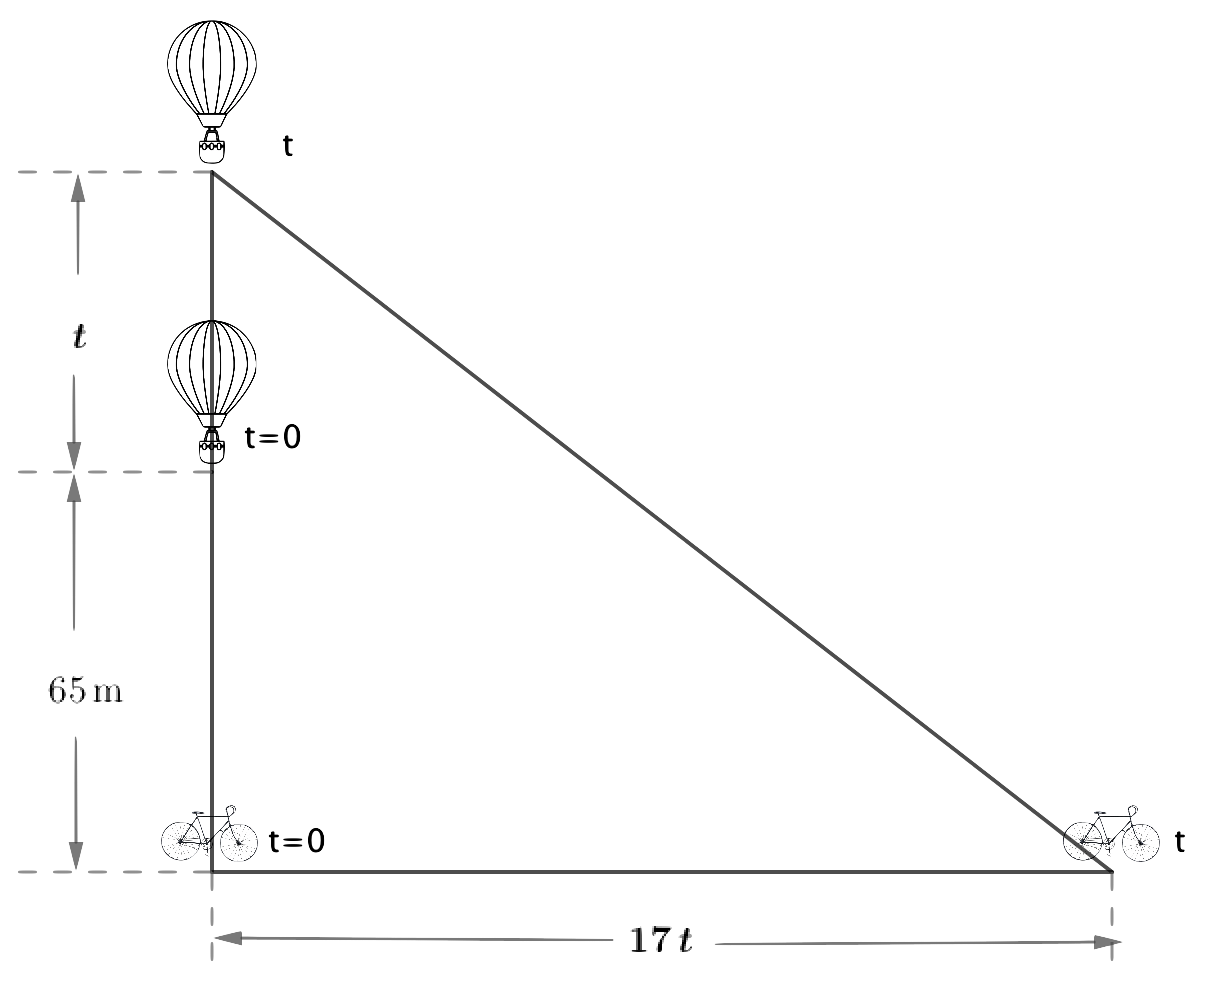
\includegraphics[width=0.5\textwidth]{imagenes/T02IM12.png}
	\end{figure}		
	\end{multicols}

\vspace{-10mm}
\color{teal!80}
\rule{200pt}{0.2pt}
\color{black}


\vspace{5mm} $ s(t)=\sqrt{(17t)^2+(65+t)^2}=\sqrt{290t^2+130t+4225}\ \mathrm{m} \, ; \quad  \ t(\mathrm{s}) \qquad  \textcolor{gris}{(t=0\leftrightarrow s=65 )}$

\vspace{5mm} $\displaystyle \eval{\dv{s}{t}\ }_{\, t=3}= \eval{\dfrac{580t+130}{2\sqrt{290t^2+130t+4225}}\ }_{\, t=3}=\, 22\, \mathrm{m\, s}^{-1}$

\end{miejercicio}

\vspace{1cm}
\begin{miejercicio}
	
	Suponga que una gota de lluvia es una esfera perfecta y que, durante la condensación, la gota recolecta humedad a una tasa proporcional al área de su superficie. Demuestre que en tales circunstancias el radio de la gota aumenta a una tasa constante.
\color{teal!80}
\rule{200pt}{0.2pt}
\color{black}
\vspace{5mm}

Esfera: $\quad V=\dfrac 4 3 \pi r^3;\qquad S=4\pi r^2\qquad \quad$ Por hipótesis: $\ \displaystyle \dv{V}{t}=k\, S$

\vspace{3mm} $\begin{cases}
\ \displaystyle \dv{V}{t}=k\, S =k\, 4\pi r^2& \text{(hipótesis)} \\ \\
\ \displaystyle \dv{V}{t}=4\pi r^2\, \dv{r}{t} 	
\end{cases} \ \to \quad 4\pi r^2 \displaystyle \ \dv{r}{t}=k\ 4\pi r^2 \ \ \Rightarrow \ \ \displaystyle \dv{r}{t}=k\ \text{(cte)}$

\end{miejercicio}


\vspace{1cm}
\begin{miejercicio}
	
Cuando la longitud $L$ del péndulo de un reloj se mantiene constante, el periodo del péndulo $T$ depende de la aceleración debida a la gravedad $g$. Por lo tanto, el periodo variará ligeramente cuando el reloj se mueva de un lugar a otro de la superficie de la Tierra, dependiendo del cambio de $g$. 
 
\vspace{2mm}La relación que liga el periodo $T$, su longitud $L$ y la gravedad del lugar $g$ viene dada por: 

$$\ T=2\pi \sqrt{\dfrac{L}{g}}$$

$\quad a)\quad $ Manteniendo  $L$ constante y  $g$ como variable, calcular $\dd T$ y usar el resultado para responder los siguientes apartados

\vspace{3mm}$\quad b)\quad $ Si $g$ aumenta, ?`$T$ aumentará o disminuirá? ?`El péndulo de un reloj irá más rápido o más lento? Razonar la respuesta. 

\vspace{3mm}$\quad c)\quad $ Un reloj con péndulo de $100 \, \mathrm{cm}$ se mueve de una localidad donde $g = 980 \, \mathrm{cm\,  seg}^{-2}$ a una nueva localidad. Esto aumenta el periodo en $\dd T = 0.001 \, \mathrm{s}$. Determinar $\dd g$ y estimar el valor de $g$ en la nueva localidad. 
	
\color{teal!80}
\rule{200pt}{0.2pt}
\color{black}
\vspace{5mm}

$\triangleright \ \ a)\quad T=2\pi \sqrt{L}\, g^{-1/2} \ \to \ \dd T=2\pi \sqrt{L}\, \left( -\dfrac 1 2  g^{-3/2}\right) \, \dd g = -\pi \sqrt{L}\, g^{-3/2}\, \dd g$

\vspace{3mm} $\triangleright \ \ b) \quad \text{Si } \ \dd g \uparrow \ \ (\dd g > 0 )\ \ \to \ \  \dd T \downarrow \ (\dd T <0)\, , \ $ el reloj atrasará (irá más lento).  

\vspace{3mm} $\triangleright \ \ c)\quad 0.001=-\pi \sqrt{100}\ (980)^{-3/2}\, \dd g \quad \to \quad \dd g \approx -0.977 \, \mathrm{cm\, s}^{-2} \quad \Rightarrow $

\vspace{3mm} $\Rightarrow \quad  \dd g \approx \Delta g = g-g_0 \ \to \ g=g_0+\dd g = 980 +(-0.977) \approx 979\, \mathrm{cm\, s}^{-2} $

\end{miejercicio}

%%%%%%%%%%%%%%%%%%%%%%%%%%%%%%%%%%%%%%%%%%

\vspace{1cm}
\begin{mipropuesto}

Sea $f(x,y)=x\sin y+y^2\cos xy$, calcular:

\vspace{5mm} \hspace{2cm} $\displaystyle f_x=\pdv{f}{x};\quad f_y, \quad f_{x,x}=\pdv[2]{f}{x};\quad f_{x,y}=\pdv[2]{f}{x}{y};\quad f_{y,x};\quad f_{y,y}$

\color{olive}
\rule{200pt}{0.2pt}
\color{black}


\begin{flushright}
		 Soluciónes: $\quad \ f_x=\sin y-y^3\sin xy;\quad f_y=x\cos y-xy^2\sin xy +2y\cos xy$
		 
		 \vspace{3mm} $f_{x,x}=-y^4 \cos xy;\quad f_{x,y}=\cos y-xy^3\cos xy-y^2\sin xy-2y^2\sin xy=f_{y,x}$
		 
		 \vspace{3mm} $f_{y,y}=-x\sin y-x^2y^2\cos xy-4xy\sin xy+2\cos xy$
\end{flushright}

\end{mipropuesto}

\vspace{1cm}
\begin{mipropuesto}

Calcular una aproximación del volumen de chapa necesaria para construir una esfera hueca de $40\, \mathrm{cm}$ de diámetro exterior y espesor de $0.2\, \mathrm{cm}$.

\color{olive}
\rule{200pt}{0.2pt}
\color{black}


\begin{flushright}
		Aproximar por la diferencial. Solución: $320\pi \, \mathrm{cm}^3$
\end{flushright}

\end{mipropuesto}


\vspace{1cm}
\begin{mipropuesto}

\begin{multicols}{2}
En un tanque cónico, el agua entra a razón de $9\, \mathrm{m}^3\, \mathrm{min}^{-1}$. El tanque está colocado con el vértice hacia abajo y tiene una altura de $10\, \mathrm{m}$ y un radio de $5\, \mathrm{m}$.

\vspace{2mm} ?`Qué tan rápido sube el nivel de agua cuando la profundidad de la misma es de $6\, \mathrm{m}$?
\begin{figure}[H]
	\centering
	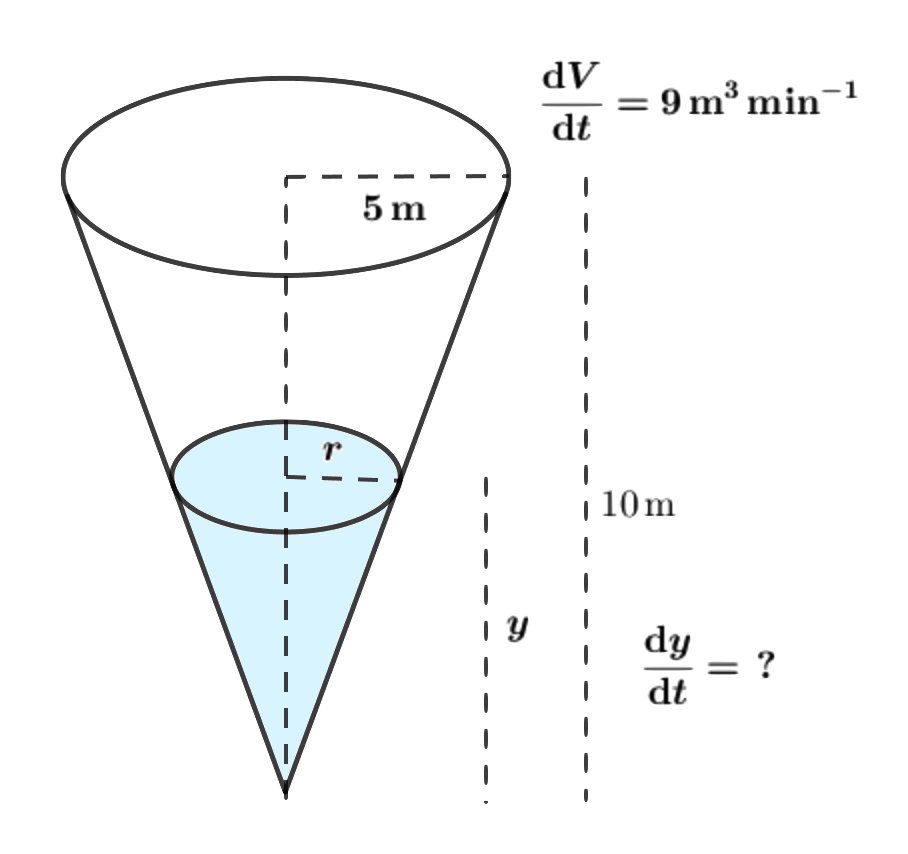
\includegraphics[width=0.3\textwidth]{imagenes/T02IM11.png}
	\end{figure}
\end{multicols}	

\color{olive}
\rule{200pt}{0.2pt}
\color{black}

\begin{flushright}
	 Solución: $\ 0.32\, \mathrm{m\, min}^{-1}$
\end{flushright}

\end{mipropuesto}





\vspace{1cm}
\begin{mipropuesto}

Se bombea gas a un globo esférico a razón de $6\mathrm{m}^3\, \mathrm{min}^{-1}$. Si la presión se mantiene constante, ?`con qué velocidad cambia el radio del globo cuando el diámetro es de $120\, \mathrm{cm}$?

\color{olive}
\rule{200pt}{0.2pt}
\color{black}


\begin{flushright}
		 Solución: $1.33 \, \mathrm{m}^3 \, \mathrm{min}^{-1}$
\end{flushright}

\end{mipropuesto}




\vspace{1cm}
\begin{mipropuesto}

Una persona camina a una velocidad constante de $3\, \mathrm{m\, s}^{-1}$ y se aleja horizontalmente, en línea recta, de una farola de $10\, \mathrm{m}$ de altura. Sabiendo que la persona mide $1.70\, \mathrm{m}$, calcúlese la velocidad de crecimiento de la sombra a los $t$ segundos de comenzar a caminar.

\color{olive}
\rule{200pt}{0.2pt}
\color{black}


\begin{flushright}
		 Solución: $\  0.614\,  \mathrm{m\, s}^{-1}$
\end{flushright}

\end{mipropuesto}




\begin{comment}

%%%%%%%%%%%%%%%%%%%%%%%%%%%%%%%%%%%. SECCIONES
\chapter{texto}
\begin{tikzpicture}
	\fill [left color=red!50, right color=teal!50] (0,0) rectangle (6.5,.2);
	\fill [left color=teal!50, right color=blue!50] (6.5,0) rectangle (11.5,.2);
	\end{tikzpicture}

\vspace{1cm}
\section{texto}
\begin{tikzpicture}
	\fill [left color=red!50, right color=teal!50] (0,0) rectangle (3.5,.1);
	\fill [left color=teal!50, right color=blue!50] (3.5,0) rectangle (7.5,.1);
	\end{tikzpicture}
\vspace{0.5cm}

\subsection{texto}
\begin{tikzpicture}
	\fill [left color=red!50, right color=teal!50] (0,0) rectangle (3.5,.01);
	\fill [left color=teal!50, right color=blue!50] (3.5,0) rectangle (7.5,.01);
	\end{tikzpicture}
\vspace{0.5cm}


%%%%%%%%%%%%%%%%%%%%%%%%%%%%%%%%%%%. \begin{ ------>. 
detsacado;  cuadro-naranja;  cuadro-gris;  miejercicio (solución extensa);  mipropuesto (solución corta y fuera del cuadro)

%%%%%%%%%%%%%%%%%%%%%%%%%%%%%%%%%%%. CURIOSIDAD
\vspace{1cm}
\color{ForestGreen!80}
\rule{250pt}{0.2pt}
Texto
\vspace{-8mm}
\begin{flushright}
\rule{250pt}{0.2pt}		
\end{flushright}	
\color{black}
\end{comment}







 %Derivadas
\chapter{La integral en física}
\setlength{\parindent}{0cm}

\begin{tikzpicture}
	\fill [left color=red!50, right color=teal!50] (0,0) rectangle (6.5,.2);
	\fill [left color=teal!50, right color=blue!50] (6.5,0) rectangle (11.5,.2);
	\end{tikzpicture}
\begin{comment}
\vspace{1cm}
\section{Uno.Uno}
\begin{tikzpicture}
	\fill [left color=red!50, right color=teal!50] (0,0) rectangle (3.5,.1);
	\fill [left color=teal!50, right color=blue!50] (3.5,0) rectangle (7.5,.1);
	\end{tikzpicture}
\vspace{0.5cm}

\vspace{1cm}
\subsection{Uno.Uno.Uno}
\begin{tikzpicture}
	\fill [left color=red!50, right color=teal!50] (0,0) rectangle (3.5,.01);
	\fill [left color=teal!50, right color=blue!50] (3.5,0) rectangle (7.5,.01);
	\end{tikzpicture}
\vspace{0.5cm}

\end{comment}\vspace{1cm}
\section{Integrales en física}
\begin{tikzpicture}
	\fill [left color=red!50, right color=teal!50] (0,0) rectangle (3.5,.1);
	\fill [left color=teal!50, right color=blue!50] (3.5,0) rectangle (7.5,.1);
	\end{tikzpicture}
\vspace{0.5cm}

\subrayado{\emph{``Una \textbf{integral} en física es la suma de muchas cosas muy pequeñas''}.}

\begin{multicols}{2}
$\quad$

El espacio recorrido por una partícula que viaja con una velocidad que depende del tiempo $v(t)$, desde un tiempo $0$ hasta un tiempo $\tau$ lo podemos calcular dividiendo el intervalo $[0,\tau]$ en pequeños intervalos de amplitud $\Delta x$ en los que podemos suponer, en cada uno de ellos, que la velocidad es constante $v_i(t)$, así, para el desplazamiento en el intervalo i-ésimo tendremos: $\ \Delta x_i=v_i(t)\, \Delta t\ $ y en todo el intervalo:
\begin{figure}[H]
	\centering
	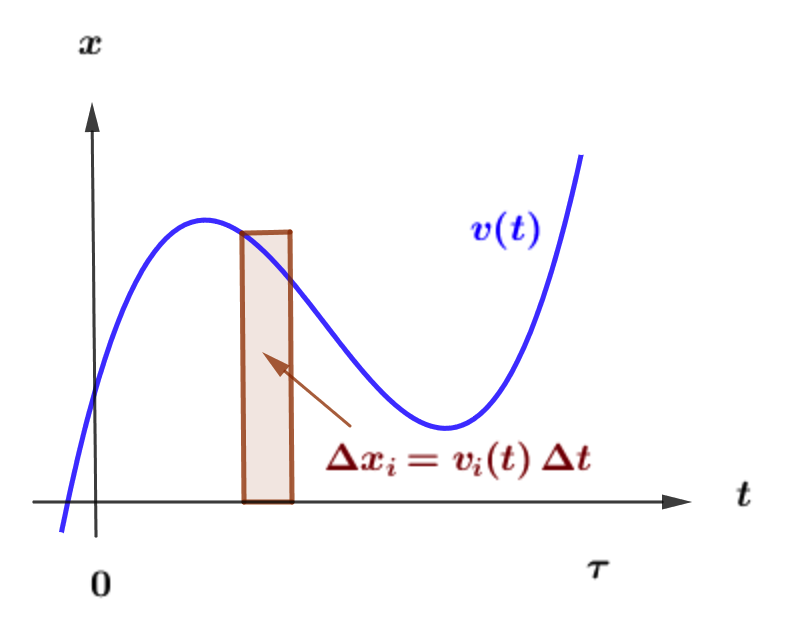
\includegraphics[width=.4\textwidth]{imagenes/T02IM02.png}
\end{figure}
\end{multicols}

$\displaystyle \Delta x=\Delta x_1+ \Delta x_2+ \cdots = \sum_{t=0}^\tau v_i(t)\, \Delta t \quad $ aproximación que será mejor cuanto menor sea $	\Delta t$

Cuando $ \ \displaystyle  \Delta t  << 1 \quad \to  \quad \Delta t \sim \dd t \to 0 \qquad \Rightarrow \qquad \Delta x \ = \ \int_0^\tau  v(t)\, \dd t$


Si $\ x(t)\ $ es una primitiva de $\ v(t)\, , \ \ \displaystyle \dv{x(t)}{t}=v(t) \quad \to \quad \displaystyle \Delta x=  \int_0^\tau  v(t)\, \dd t = \left[\,  x(t) \, \right]_0^\tau=x(\tau)-x(0) \quad$ (Barrow).

Ecuación que se puede escribir como $\quad\displaystyle x(t)\ = \ x(0) \ + \ \int_0^t  v(t')\, \dd t' \ $

\textcolor{gris}{$\displaystyle \int_0^t  v(t')\, \dd t' =\int_0^t  v(x)\, \dd x =\int_0^t  v(z)\, \dd z\, ;  \quad t',\, x,\, z\ $ variables mudas. } 

\vspace{5mm}\emph{En física todas las integrales son definidas.}

\vspace{5mm}\ul{Ejemplos:}

\hspace{1cm} \vspace{3mm} $\triangleright \displaystyle \quad \rho=\dv{m}{V} \ \to \ \dd m = \rho\, \dd V  \quad \Rightarrow \quad M=\int_M \dd m = \int_V \rho\, \dd V$

\hspace{1cm} \vspace{3mm} $\triangleright \displaystyle \quad \overrightarrow E=\dv{\overrightarrow F}{q} \ \to \ \dd \overrightarrow F = \overrightarrow E \, \dd q \quad \Rightarrow \quad \overrightarrow F = \int_Q \overrightarrow E \, \dd q$

\hspace{1cm} \vspace{3mm} $\triangleright \displaystyle \ \ \, \text{ Trabajo elemental: } \  \dd W = \overrightarrow F \cdot \dd \vec r \quad \Rightarrow \quad W=\int_A^B \overrightarrow F \cdot \dd \vec r$ 

\vspace{5mm} Dimensionalmente, al ser la integral una suma, sus dimensiones serán el producto de las dimensiones del integrando por las del diferencial. $\quad$ \textcolor{gris}{$(\ [W]=[F][\dd r]=\mathrm N \, \mathrm m \ ) $ }

\vspace{1cm}
Se define el \textbf{valor medio de una función} en un intervalo [a,b]:
\begin{multicols}{2}
$\quad$

$\qquad  <\, f(x)\,> \ = \ \displaystyle \dfrac 1 {b-a}\, \int_a^b f(x), \dd x $

\begin{figure}[H]
	\centering
	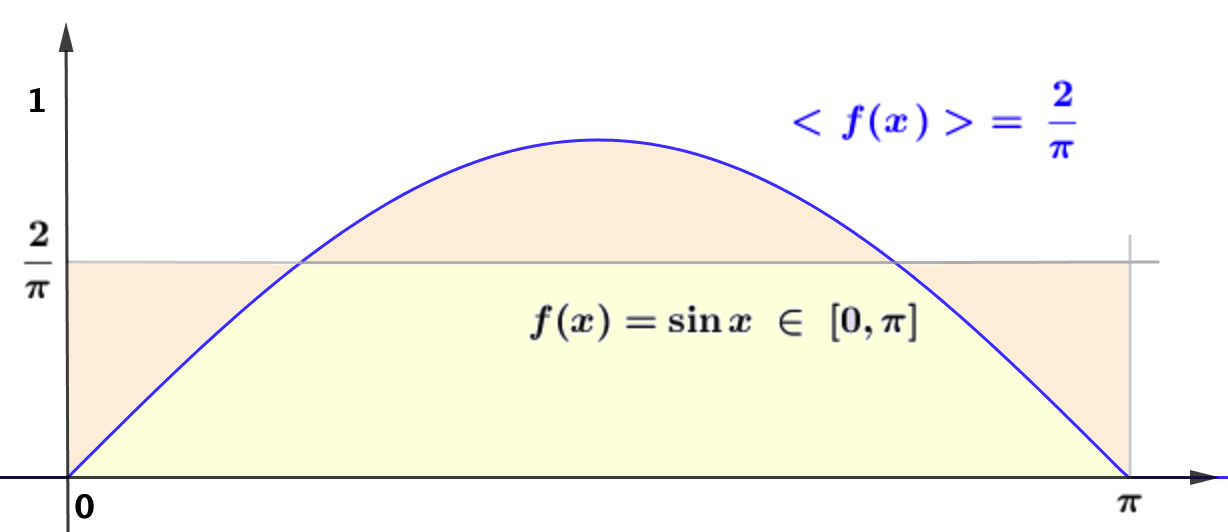
\includegraphics[width=.4\textwidth]{imagenes/T02IM04.png}
\end{figure}
\end{multicols}

Dada $\ \displaystyle \int_a^b f(x)\, \dd x \, , \ $ si alguno de los límites de integración en $\infty$ o bien la función diverge a $\infty$ en $]a,b[$, se dice que tenemos una \textbf{integral impropia}, que se estudia en el apéndice \ref{integrales-impropias}. 

\vspace{10mm}

\begin{miejercicio}
	
La función $\rho (x)=300 \left[ 2+\sin(4\sqrt{x+0.15}) \right]$ da la densidad de coches (en número de coches por $\mathrm{km}$) en los primeros $20\; \mathrm{km}$ de una autovía, siendo $x$ la distancia en $\mathrm{km}$ al comienzo de la misma. Calcula el número total de coches en ls $20 \; km$.  

\rule{200pt}{0.1pt}

\vspace{3mm}
	
	$\displaystyle \int_0^{20} \rho (x) \; \dd x= \int_0^{20} 300 \left [2+\sin(4\sqrt{x+0.15}) \right]   \; \dd x$
	$\displaystyle = 600 \int_0^{20} \dd x + 300 \int_0^{20}  \sin (4\sqrt{x+0.15}) \; \dd x = 
	CV:\; \left[ \begin{matrix} \sqrt { x+0.15 } =t \\ \dd x=2t\quad \dd t \end{matrix} \right] \to $
	$ \; =\cdots\; $ (\textcolor{gris}{Acábese}) $ \cdots   =11513 \text{ coches } $
\end{miejercicio}	
	
	
\vspace{5mm}

\begin{miejercicio}
	
Sobre una partícula situada a $x\; \mathrm{m}$ del origen, actúa una fuerza $F=(3x^2+2x)\; \mathrm{N}$. ?`Qué trabajo realiza dicha fuerza al mover la partícula desde la posición $x=1$ hasta $x=5\; \mathrm{m}$
	
\rule{200pt}{0.1pt}

\vspace{3mm}
	
	Us resultado de física asegura que el trabajo $W$ que realiza un cuerpo sometido a una fuerza $F$ desde $x=x_1$ hasta $x= x=2$ es  $\; W=\displaystyle \int_{x_1}^{x_2} F \cdot \dd x $, luego:
	
	$W=\displaystyle \int_1^5 (3x^2+2x)\; \dd x = \eval[x^3+x^2|_1^5=(5^3+5^2)-(1+1)= 148\; \mathrm{J}$. 
	
	\vspace{2mm}\textcolor{gris}{$\mathrm{J}$ es la unidad física de trabajo, $\mathrm{N}\cdot \mathrm{m}$}

\end{miejercicio}
	
	\vspace{5mm}

\begin{miejercicio}

Calcula la posición de un móvil sabiendo que se desplaza rectilineamente con a aceleración constante igual a $a=8 \; \mathrm{m}\cdot \mathrm{s}^{-2}$ y que su velocidad es $0\; \mathrm{m}\cdot \mathrm{s}^{-1}$ cuando $t=3 \; \mathrm{s}$ y que se encuentra en el origen de coordenadas a los $11 \; \mathrm{s}$
	
\rule{200pt}{0.1pt}

\vspace{3mm}
	
	Sea $s(t)$ la posición del móvil a los $t\; \mathrm{s}$. Por física sabemos que: $ \displaystyle \  v(t)=s'(t)=\frac {\dd s(t)}{\dd t}\; $ y $\; a(t)=s''(t)=\dfrac {\dd^2 s(t)}{\dd t^2}=8\; \mathrm{m}\cdot \mathrm{s}^{-2}$
	
\vspace{2mm}	Calculemos la velocidad: $\ \ \displaystyle v(t)=\int a(t)\; \dd t = \int 8 \, \dd t =8t +\mathcal {C}_1\; $; como $v(3)=0=24+\mathcal {C}_1 \to  \mathcal {C}_1=-24 \Rightarrow v(t)=8t-24 \ (\mathrm{m}\, \mathrm{s}^-1)$
	
\vspace{2mm}	Calculemos, ahora, la posición: $\ \ \displaystyle s(t)=\int v(t)\; \dd t = \int (8t-24)\; \dd t = 4t^2 -24t +\mathcal {C}_2\; $; como $s(11)=0=220+\mathcal {C}_2 \to \mathcal{C}_2=-220 \Rightarrow s(t)=4t^2-24t-220 \ (\mathrm{m})$ 
	
\end{miejercicio}








\section{Integrales impropias}	
\label{integrales-impropias}

\begin{tikzpicture}
	\fill [left color=red!50, right color=teal!50] (0,0) rectangle (6.5,.2);
	\fill [left color=teal!50, right color=blue!50] (6.5,0) rectangle (13.5,.2);
	\end{tikzpicture}


\vspace{1cm}


El concepto de integral definida puede extenderse a límites de integración infinitos del siguiente modo:
$\qquad \displaystyle \int_a^{+\infty} f(t)\; \dd t = \underset{x\to + \infty}{lim}\;{\int_a^x f(t)\; \dd t}$

\begin{miejercicio}

Calcula: $a) \quad \displaystyle \int_1^{+\infty} \dfrac {1}{t^2} \dd t\; ; \qquad \quad b) \quad \displaystyle \int_1^{+\infty} \dfrac 1 t \dd t $	

$a)\quad \displaystyle \int_1^x \dfrac {1}{t^2} \dd t= \eval[-\dfrac{1}{x}|_1^x=-\dfrac 1 x + 1 \Rightarrow \; \;  \displaystyle \int_0^{+\infty} \dfrac {1}{t^2}\; \dd t = \underset{x\to + \infty}{lim}\;{-\dfrac 1 x + 1}=1$

$b) \quad \displaystyle \int_1^x \dfrac 1 t \dd t = \eval[\mathrm{ln}\abs{x}|_1^x=\mathrm{ln}x-\cancelto{0}{\mathrm{ln}1}=\mathrm{ln}x \Rightarrow \;\; \displaystyle \int_1^{+\infty} \dfrac {1}{t}\; \dd t = \underset{x\to + \infty}{lim}\;{\mathrm{ln}x}=+\infty$

\begin{figure}[H]
 	\centering
	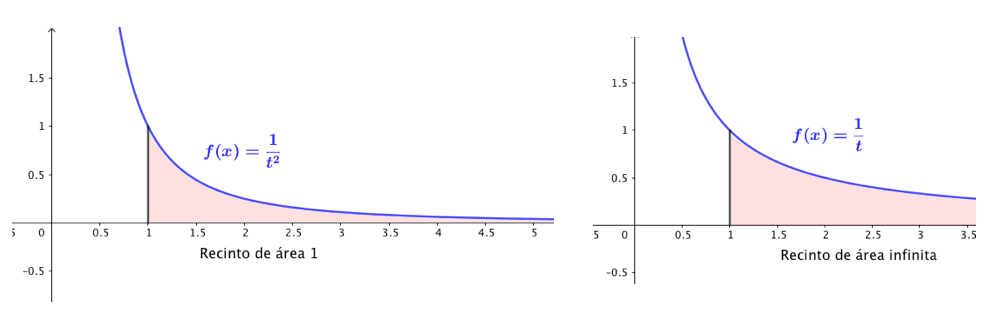
\includegraphics[width=1\textwidth]{imagenes/IMPROPIAS/T08IM10.png}
\end{figure}

\vspace{4mm} \end{miejercicio}

\vspace{4mm} \textbf{Otras integrales impropias:}



Si $f$ no está acotada en $[a,b]$ (discontinuidad asintótica o de salto infinito), en general, la $\displaystyle \int_a^b f(t) \dd t$ no existe. Sin embargo, en algunos casos, se puede proceder de forma análoga al caso anterior. Si por ejemplo $f$ presenta una discontinuidad de salto infinito en $c\in[a,b]$:

$$\displaystyle \int_a^b f(t) \dd t= \underset {x\to c^-}{lim}{\int_a^x f(t) \dd t}-\underset {x\to c^+}{lim}{\int_x^b f(t) \dd t}$$


\vspace{4mm} \begin{miejercicio}

Calcula: $a) \quad \displaystyle \int_0^1 \dfrac {1}{\sqrt{t}} \dd t\; ; \qquad \quad b) \quad \displaystyle \int_0^1 \dfrac {1} {t^2} \dd t $	

$a) \quad \displaystyle \int_0^1 \dfrac {1}{\sqrt{t}} \dd t= \underset {x\to 0^+}{lim}{\int_x^1 \dfrac {1}{\sqrt{t}} \dd t} =\underset {x\to 0^+}{lim} { \eval[2\sqrt{t}|_x^1 }= \underset {x\to 0^+}{lim} {2-2\sqrt{x}}=2$

$b) \quad  \displaystyle \int_0^1 \dfrac {1} {t^2} \dd t = \underset {x\to 0^+}{lim}{\int_x^1 \dfrac {1}{t^2} \dd t}= \underset {x\to 0^+}{lim} { \eval[-\dfrac 1 t|_x^1 }=\underset {x\to 0^+}{lim} {\left(-1+\dfrac 1 x  \right)}=+\infty$

\begin{figure}[H]
 	\centering
	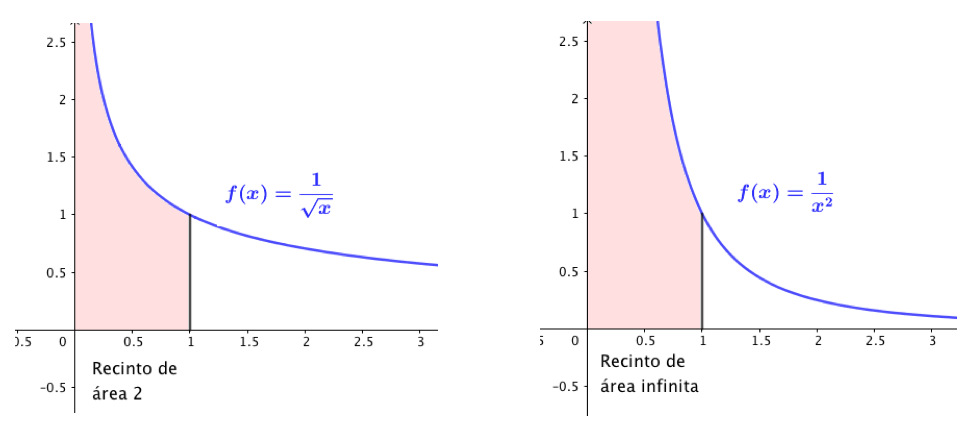
\includegraphics[width=0.75\textwidth]{imagenes/IMPROPIAS/T08IM11.png}
\end{figure}

\end{miejercicio}

\vspace{4mm} Resumiendo:

En cálculo, una integral impropia es el límite de una integral definida cuando uno o ambos extremos del intervalo de integración se acercan a un número NO real específico,  o a $\pm \infty$.

Además una integral definida es impropia cuando la función integrando de la integral definida tiene discontinuidad infinita en el intervalo de integración. 

También se pueden dar ambas situaciones.


\vspace{1cm}


\begin{miejercicio}


	Calcula $\ \ \displaystyle \int_0^1 \dfrac 1 x \; \dd x$
\vspace{3mm}

\rule{200pt}{0.1pt}

\vspace{2mm}	
	
	$\displaystyle \int_x^1 \dfrac 1 x \; \dd x= \eval[\mathrm{ln}\abs {x}|_x^1=  \cancelto{0}{\mathrm{ln} 1}- \mathrm{ln} |x|=-\mathrm{ln} |x| \Rightarrow $
	$\displaystyle \int_0^1 \dfrac 1 x \; \dd x= \underset {x\to 0^+}{lim }{(-\mathrm{ln} x)} =+\infty $
	
	Esta integral ' impropia' es divergente, la integral no existe.
	
\end{miejercicio}

\vspace{4mm}
\begin{miejercicio}
	
	Calcula $\displaystyle \int_0^{\infty} \dfrac {1}{1+x^2}\; \dd x$
\vspace{3mm}

\rule{200pt}{0.1pt}

\vspace{2mm}

$\displaystyle \int \dfrac {1}{1+t^2}\; \dd t = \arctan x + \mathcal C \quad \to \quad \displaystyle \int_0^{\infty} \dfrac {1}{1+x^2}\; \dd x=\eval[\arctan x|_0^{\infty}= $
$\underset {x\to \infty}{lim} \left[ (\arctan x) - (0) \right]$
$=\underset {x\to \infty}{lim}{\arctan x}=\dfrac {\pi}{2}$

\end{miejercicio}

\vspace{4mm}

\begin{miejercicio}
	Calcula, si existen, las siguientes integrales impropias.
	
	\begin{multicols}{2}
	\begin{enumerate}[a) ]
	\item $\displaystyle \int_{-\infty}^{+\infty} \dfrac {1}{1+x^2} \; \dd x$
	\item $\displaystyle \int_{-\infty}^{0} e^x \; \dd x$
	\item $\displaystyle \int_{0}^{1} \dfrac {1}{\sqrt[3]{x}} \; \dd x$
	\item $\displaystyle \int_{0}^{1} \dfrac {1}{\sqrt{1-x^2}} \; \dd x$
	\end{enumerate}
	\end{multicols}


\rule{200pt}{0.1pt}

\vspace{3mm}	


\vspace{4mm} $a) \quad \displaystyle \int_{-\infty}^{+\infty} \dfrac {1}{1+x^2} \; \dd x=I_a$

\vspace{2mm} Calculemos $\displaystyle \int_{-x}^{+x} \dfrac {1}{1+t^2} \; \dd t= \eval[\arctan x|_{-x}^x=\arctan x - \arctan(-x)\quad \ { con } \; x>0$

\vspace{2mm} Luego $\displaystyle I_a= \underset{x\to +\infty}{lim}\;{\left[ arctan x - \arctan(-x) \right] } = \pi/2 - (-\pi/2)=\pi$


\vspace{4mm} $b) \quad \displaystyle \int_{-\infty}^{0} e^x \; \dd x=I_b$

\vspace{2mm} Calculemos $\displaystyle \int_{-x}^{0} e^t \; \dd t= \eval [e^t|_{-x}^0= 1-e^{-x}$

\vspace{2mm} Luego $\displaystyle I_b=$
$\underset {x\to + \infty}{lim}{(1-e^{-x})}=$
$\underset {x\to + \infty}{lim}{\left(1-\dfrac {1}{e^x}\right)}=1-0=1$


\vspace{4mm} $c) \quad \displaystyle \int_{0}^{1} \dfrac {1}{\sqrt[3]{x}} \; \dd x=I_c$

\vspace{2mm} Como la función tiene discontinuidad asintótica en $x=0$, calculemos primero:

\vspace{2mm} $\displaystyle \int_{x}^{1} \dfrac {1}{\sqrt[3]{x}} \; \dd x= =\int_{x}^{1} x^{-1/3} \; \dd x=3/2\;  \eval[x^{2/3}|_x^0= 3/2\; (1-x^2/3)$

\vspace{2mm} Luego: $\displaystyle I_c=3/2 \; \underset{x\to 0^+}{lim}\; {1-x^{2/3}}= 3/2$


\vspace{4mm} $d) \quad \displaystyle \int_{0}^{1} \dfrac {1}{\sqrt{1-x^2}} \; \dd x= I_d$

\vspace{2mm} Función discontinua asintótica en $x=1$, calculemos:

\vspace{2mm} $\displaystyle \int_{0}^{x} \dfrac {1}{\sqrt{1-x^2}} \; \dd x= \eval [\arcsin x|_0^x= \arcsin x - 0 = \arcsin x$

\vspace{2mm} Luego: $\displaystyle I_d=\underset {x\to 1^-}{lim}\;{\arcsin x}= \pi/2$
\end{miejercicio}


%%%%%%%%%%%%%%%%%%%%%%%%%%%%%%%%%%%%%%%%%%%%%%%%%%%%%%%%%%%%%
\vspace{5mm}

\begin{miejercicio}

Calcula, si existen, las siguientes integrales impropias.
\begin{multicols}{2}
\begin{enumerate}[a) ]
\item $\displaystyle \int_{0}^{+\infty} e^{-x}\; \sin x \; \dd x\; $ (Partes)
\item $\displaystyle \int_{-\infty}^1{} x\; e^x \;  \dd x\; $ (Partes)
\item $\displaystyle \int_{1}^{+\infty} \cos x \;  \dd x\; $ (Inmed.)
\item $\displaystyle \int_{4}^{+\infty} \dfrac {1}{x^2-4}\;  \dd x\; $ (Racional)
\item $\displaystyle \int_{1}^{+\infty} \dfrac 1 x \;  \dd x\; $ (Inmed.)
\item $\displaystyle \int_{-\infty}^{-2} \dfrac 1 {x^2} \;  \dd x\; $ (Inmed.)
\item $\displaystyle \int_{0^+}^{e} \dfrac {\mathrm{ln} x}{\sqrt{x}} \;  \dd x\; $ (Discont: $0$; Partes)
\item $\displaystyle \int_{0^+}^{1} x\; \mathrm{ln} x \;  \dd x\; $ (Discont: $0$; Partes)
\end{enumerate}	
\end{multicols}

\rule{200pt}{0.1pt}

\vspace{3mm}

\textcolor{gris}{Sol: $a)\;1/2;\quad b); 0;\quad c)\; \nexists; \quad d)\; (\mathrm{ln}2)/2; \quad e); \nexists; \quad f); 1/2; \quad g)\; -\sqrt{e}; \quad h)\; -1/4 $}
\end{miejercicio}







\begin{comment}

%%%%%%%%%%%%%%%%%%%%%%%%%%%%%%%%%%%. SECCIONES
\chapter{texto}
\begin{tikzpicture}
	\fill [left color=red!50, right color=teal!50] (0,0) rectangle (6.5,.2);
	\fill [left color=teal!50, right color=blue!50] (6.5,0) rectangle (11.5,.2);
	\end{tikzpicture}

\vspace{1cm}
\section{texto}
\begin{tikzpicture}
	\fill [left color=red!50, right color=teal!50] (0,0) rectangle (3.5,.1);
	\fill [left color=teal!50, right color=blue!50] (3.5,0) rectangle (7.5,.1);
	\end{tikzpicture}
\vspace{0.5cm}

\subsection{texto}
\begin{tikzpicture}
	\fill [left color=red!50, right color=teal!50] (0,0) rectangle (3.5,.01);
	\fill [left color=teal!50, right color=blue!50] (3.5,0) rectangle (7.5,.01);
	\end{tikzpicture}
\vspace{0.5cm}


%%%%%%%%%%%%%%%%%%%%%%%%%%%%%%%%%%%. \begin{ ------>. 
detsacado;  cuadro-naranja;  cuadro-gris;  miejercicio (solución extensa);  mipropuesto (solución corta y fuera del cuadro)

%%%%%%%%%%%%%%%%%%%%%%%%%%%%%%%%%%%. CURIOSIDAD
\vspace{1cm}
\color{ForestGreen!80}
\rule{250pt}{0.2pt}
Texto
\vspace{-8mm}
\begin{flushright}
\rule{250pt}{0.2pt}		
\end{flushright}	
\color{black}
\end{comment}




 %Integrales
\chapter{Desarrollos en serie de \emph{Taylor}}
\label{DSTaylor}
\setlength{\parindent}{0cm}

\begin{tikzpicture}
	\fill [left color=red!50, right color=teal!50] (0,0) rectangle (6.5,.2);
	\fill [left color=teal!50, right color=blue!50] (6.5,0) rectangle (11.5,.2);
	\end{tikzpicture}


\begin{comment}
\vspace{1cm}
\section{Uno.Uno}
\begin{tikzpicture}
	\fill [left color=red!50, right color=teal!50] (0,0) rectangle (3.5,.1);
	\fill [left color=teal!50, right color=blue!50] (3.5,0) rectangle (7.5,.1);
	\end{tikzpicture}
\vspace{0.5cm}

\vspace{1cm}
\subsection{Uno.Uno.Uno}
\begin{tikzpicture}
	\fill [left color=red!50, right color=teal!50] (0,0) rectangle (3.5,.01);
	\fill [left color=teal!50, right color=blue!50] (3.5,0) rectangle (7.5,.01);
	\end{tikzpicture}
\vspace{0.5cm}

\end{comment}




\section{Polinomios de \emph{Taylor}}
\begin{tikzpicture}
	\fill [left color=red!50, right color=teal!50] (0,0) rectangle (3.5,.1);
	\fill [left color=teal!50, right color=blue!50] (3.5,0) rectangle (7.5,.1);
	\end{tikzpicture}
\vspace{0.5cm}


Con la diferencial obtenemos la primera aproximación de una función: es la recta que más se aproxima a la función en un punto.



\begin{multicols}{2}
$\Delta f \approx \dd f=f'(x)\, \dd x \ \to \ $

$\quad$

$\to \ f(x)-f(x_0)\approx f'(x_0) (x-x_0) \ \ \Rightarrow \ \ $

$\quad$

$\Rightarrow \ \  f(x)\ \approx \ f(x_0)\ + \ f'(x_0) (x-x_0) $



\begin{figure}[H]
	\centering
	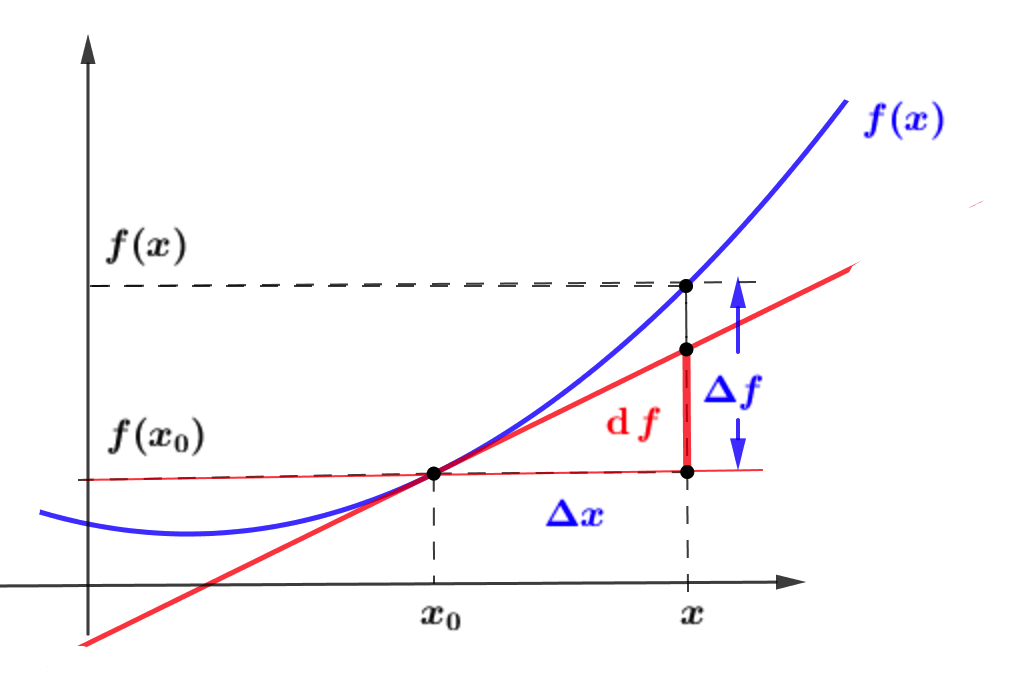
\includegraphics[width=.45\textwidth]{imagenes/T02IM03.png}
\end{figure}	
\end{multicols}

Acabamos de ver que $\ \ f(x)-f(x_0) = \Delta x \ $ cuando $\ x\to x_0 \ $, es decir, cuando $\ x-x_0= \dd x\ $ tenemos que \textcolor{gris}{(la diferencial como aproximación del cambio de una función)}: 

\vspace{-3mm}
$$\subrayado{\ \boxed{ \  \boldsymbol {\Delta f \ \approx  \  f'(x)\dd x \  = \ \dd f} \ } \ }$$

Expresión que podemos escribir como:
$\ \  f(x)\ \approx \ f(x_0)\ + \ \dfrac 1 {1!} \, f'(x_0) (x-x_0)^1$

Este concepto se puede generalizar y preguntarnos por cuál será el polinomio de segundo, o de tercer grado, que más se aproxima a la función, resultando que estos son, respectivamente:

\hspace{1cm} $\displaystyle
f(x)\ \approx \ f(x_0)\ + \ \dfrac 1 {1!} \, f'(x_0) (x-x_0)^1 \ + \ \dfrac 1{2!}\, f''(x_0)\, (x-x_0)^2 $

\hspace{1cm} $\displaystyle
f(x)\ \approx \ f(x_0)\ + \ \dfrac 1 {1!} \, f'(x_0) (x-x_0)^1 \ + \ \dfrac 1{2!}\, f''(x_0)\, (x-x_0)^2 \ + \ \dfrac 1{3!} \, f'''(x_0)\, (x-x_0)^3$



\vspace{5mm} El polinomio de orden $n$ que más se aproxima a una función $f(x)$ entorno a un punto $x_0$ es el \textbf{polinomio de Taylor} (Ver `Ampliación' en siguientes secciones):

$$\displaystyle
f(x)\ \approx \ f(x_0)\ + \ \dfrac 1 {1!} \, f'(x_0) (x-x_0)^1 \ + \ \dfrac 1{2!}\, f''(x_0)\, (x-x_0)^2 \  + \ \cdots \ + \ \dfrac 1{n!} \, f^{n)}(x_0)\, (x-x_0)^n$$

En notación de Leibniz,

$$\displaystyle \boxed{ \ \subrayado{ \ 
f(x)\ \approx \ f(x_0)\ + \ \dfrac 1 {1!} \, \eval{\dv{f}{x}}_{x_0} (x-x_0)^1 \ + \ \dfrac 1{2!}\, \eval{\dv[2]{f}{x}}_{x_0}(x-x_0)^2 \  + \ \cdots \ + \ \dfrac 1{n!} \,\eval{\dv[n]{f}{x}}_{x_0}(x-x_0)^n \ } \ }$$

A medida que aumenta el orden del desarrollo disminuye el error cometido en la aproximación.

Determinado el error máximo admisible que se comete al tomar $f(x)$ por el polinomio de Taylor, se puede determinar cuál ha de ser el grado $n$ del polinomio a considerar.

\vspace{10mm}

\begin{cuadro-naranja}
	
\color{gris}	
\textbf{Desarrollos más usuales} y radios de convergencia (zona de validez o aplicabilidad):
\begin{adjustwidth}{20pt}{0pt}
\begin{itemize}
	\item $(1+x)^n=\left( \begin{matrix} n \\ 0 \end{matrix} \right) +\left( \begin{matrix} n \\ 1 \end{matrix} \right) x+\left( \begin{matrix} n \\ 2 \end{matrix} \right) x^2+\left( \begin{matrix} n \\ 3 \end{matrix} \right) x^3+\cdots =\displaystyle \sum _{ k=0 }^{ n }{ \left( \begin{matrix} n \\ k \end{matrix} \right) { x }^{ k } } \quad -1<x<1 \ $ \begin{tiny} Binomio Newton \end{tiny}
	
	\item $e^x=1+x+\dfrac{x^2}{2!}+\dfrac{x^3}{3!}+\dfrac{x^4}{4!}+\cdots \qquad -\infty < x < +\infty$
	\item $\mathrm{ln}\; (1+x)=x-\dfrac{x^2}{2}+\dfrac{x^3}{3}-\dfrac{x^4}{4}+\dfrac{x^5}{5}- \cdots \qquad -1 < x \le 1 $
	
	\item $\dfrac{1}{1+x}=1-x+x^2-x^3+x^4-x^5+\cdots \qquad -1<x<1$
	
	\item $\sqrt{1+x} = 1 + \dfrac 1 2 x -\dfrac 1 {24} x^2 + \dfrac {13}{246}x^3- \cdots \qquad -1<x\le 1 $
	\item $\sin x = x -\dfrac{x^3}{3!}+\dfrac{x^5}{5!}-\dfrac{x^7}{7!}+\cdots \qquad -\infty < x < +\infty$
	\item $\cos x = 1 -\dfrac{x^2}{2!}+\dfrac{x^4}{4!}-\dfrac{x^6}{6!}+\cdots \qquad -\infty < x < +\infty$
	
	\item $\arctan x=x - \dfrac {x^3}{3} +\dfrac {x^5}{5}-\dfrac {x^7}{7}+\cdots \qquad x^2<1$	
	
\end{itemize}

\vspace{5mm} Para $\ |x|<<1\ $ son válidas las aproximaciones:

\vspace{-8mm}
$$(1+n)^n\approx 1+nx\, ; \qquad e^x\approx 1+x\, ; \qquad \ln(1+x)\approx x\, ; $$

$$\sin x  \approx x\, ; \qquad \cos x\approx 1\, ; \qquad \tan x\approx x$$

\begin{small}
Casos particulares frecuentes: $\qquad \boxed{ \dfrac 1{\sqrt{1-x^2}}}\  = (1-x^2)^{-1/2} \approx  1+\left(- \dfrac 1 2 \right) \, (-x^2)\ \boxed{ \approx 1+\dfrac 1 2 x^2}$

\hspace{5.2cm} $\boxed{ \ \dfrac 1{\sqrt{1\pm x}} \ } \ =(1\pm x)^{-1/2}\approx 1+	\dfrac{-1}2 (\pm x)=\  \boxed{ \ 1\mp x \ }$
\end{small}


\end{adjustwidth}
\end{cuadro-naranja}
\color{black}


\vspace{1cm}
\begin{miejercicio}

\color{gris}
\begin{multicols}{2}
Aproximación de pequeños ángulos.

\vspace{3mm}Estudio del péndulo simple.


\color{teal!80}
\rule{200pt}{0.2pt}
\color{gris}
\vspace{5mm}

$F_{neta}=-mg\sin \theta =mga_t$

\vspace{3mm}$s=\theta L \ \to \displaystyle \dv[2]{a}{t}=L\dv[2]{\theta}{t}$

\vspace{3mm} $\displaystyle L \dv[2]{\theta}{t}=-g\sin \theta \ \to \ \dv[2]{\theta}{t}+\dfrac g L\sin \theta=0$

\vspace{3mm} Ecuación que no es la de un MRUA por la presencia del factor $\sin \theta$, pero, para \textbf{ángulos pequeños}, usando polinomios de Taylor de orden uno, $\sin \theta \approx \theta$


\begin{figure}[H]
	\centering
	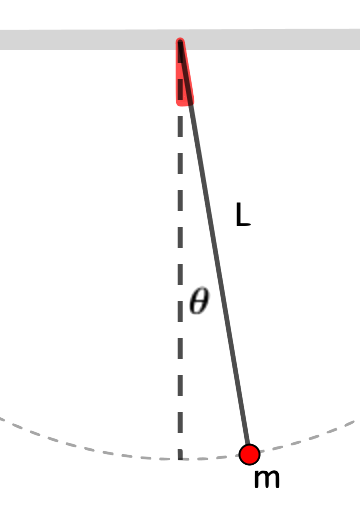
\includegraphics[width=0.35\textwidth]{imagenes/T02IM07.png}
	\end{figure}
\end{multicols}	


Para ángulos pequeños, $\ \ \displaystyle \sin \theta \approx \theta \quad \to \quad \dv[2]{\theta}{t}+\dfrac g L \theta=0$ es una ecuación diferencial de segundo órden cuya solución general es:
$\quad \theta = \theta_0 \sin(\omega t+\phi),\quad $ con $\  \omega=\sqrt{\dfrac{g}{l}}\ \ $ y $\  \ \theta_0,\, \phi $ son las amplitud y fase iniciales. 
\end{miejercicio}

%%%%%%%%%%%%%%%%%%%%%%%%%%%%%%%%%%%%%%%%%%%%%%%%%%%%%%%%%%%%%%%%%%%%%%%%%%%

\vspace{1cm}

\begin{Huge}
AMPLIACIÓN	
\end{Huge}\normalsize{.}\footnote{Capítulo extraído del libro \emph{``Cálculo infinitesimal (avanzado) para Bachillerato'' }, de 	\textsf{Ignacio Vallés Oriola}. A disposición del lector/a en \textcolor{NavyBlue}{https://igvaori.github.io}}


\vspace{1cm}

\section{Preliminares Introducción a las series de potencias}
\begin{tikzpicture}
	\fill [left color=red!50, right color=teal!50] (0,0) rectangle (3.5,.1);
	\fill [left color=teal!50, right color=blue!50] (3.5,0) rectangle (7.5,.1);
	\end{tikzpicture}
\vspace{0.5cm}

%%%%%%%%%%%%%%%%%%%%%%%%%%%%%%%%%%
Una \emph{serie de potencias} en torno al punto $x_0$ es una expresión del tipo:
\begin{equation*}
	\label{serie-potencias}
	\sum _{ k=0 }^{ \infty }{a_n(x-x_0)^n}=a_0+a_1(x-x_0)+a_2(x-x_0)^2+a_3(x-x_0)^3+\cdots 
\end{equation*}

Donde $x$ es una variable y los coeficientes $a_n$ son constantes. Se dice que una serie de potencias `converge' en el punto $x=r$  si $\underset{N\to \infty}{lim }\;{\sum _{ k=0 }^{ N }{a_n(x-r)^n}}$ existe y es finito. En caso contrario se dice que la serie es divergente.

Obviamente, la serie de potencias \ref{serie-potencias} es convergente en $x=x_0$, ya que: 

$\sum _{ k=0 }^{ \infty }{a_n(x-x_0)^n}=a_0+0+0+\cdots =a_0$

	\begin{multicols}{2}
	Pero, ¿qué se puede decir de la convergencia de la serie \ref{serie-potencias} para otros valores de x?: las series de potencias convergen en un cierto intervalo de centro $x_0$ y diverge fuera de él. 

	Para cada serie de potencias existe un número $\rho; (0\le \rho \le  \infty)$, llamado `radio de convergencia', de modo que la serie converge para $|x-x_0|<\rho$ y diverge para $|x-x_0|>\rho$. Si $\rho=\infty$, la serie de potencias converge para todo $\mathbb R$; si $\rho=0$, la serie solo converge en $x_0$.
	\begin{figure}[H]
		\centering
		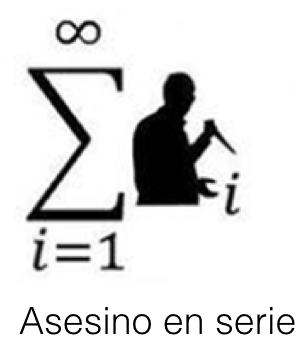
\includegraphics[width=0.15
	\textwidth]{imagenes/Taylor/xiste06.png}
	\end{figure}
	

\end{multicols}




Existen distintos \emph{criterios} para determinar si una serie es o no convergente y cual es su radio de convergencia, citamos, entre otros:
\begin{itemize}
	\item \emph{Criterio del cociente: } Si $\underset {n\to \infty}{lim}{\left| \dfrac {a_{n+1}}{a_n} \right|}=L$, donde $0\le L \le \infty$, entonces el radio de convergencia de la serie de potencias $\sum _{ k=0 }^{ \infty }{a_n(x-x_0)^n}$ es $\rho=\dfrac 1 L\, , \ $ con $\rho=\infty \leftrightarrow L=0 \quad \wedge \quad \rho=0 \leftrightarrow L=\infty\, . \ \ $
	Si este límite no existe, no podemos asegurar nada., hay que usar otros criterios.
	\item \emph{Criterio de la raíz: } Si $\underset{n\to \infty}{lim}{\sqrt[n]{|a_n|}}=L$,  con  $ 0\le L \le \infty$, entonces, el radio de convergencia de la serie de potencias $\sum _{ k=0 }^{ \infty }{a_n(x-x_0)^n}$ es, también  $\rho=1/L$, con las mismas observaciones anteriores.
\end{itemize} 

\vspace{10mm}%%%%%%%%%%%%%%%%%%%%%%%%
\section[Introducción a los desarrollos de \emph{Taylor} y \emph{MacLaurin}]{Introducción a los desarrollos de \emph{Taylor} y \emph{MacLaurin} \sectionmark{Intro. desarrollo \emph{Taylor}}}
\sectionmark{Intro. desarrollo \emph{Taylor}}

\begin{tikzpicture}
	\fill [left color=red!50, right color=teal!50] (0,0) rectangle (3.5,.1);
	\fill [left color=teal!50, right color=blue!50] (3.5,0) rectangle (7.5,.1);
	\end{tikzpicture}
\vspace{0.5cm}

Puesto que este tema excede del temario usual de un curso de segundo de bachillerato, se ha optado por hacer su exposición más sencilla (no en la forma usual definiciones-teoremas) aún perdiendo un poco el rigor matemático en favor de la facilidad expositiva.

En este tema estudiaremos la aproximación de una función $f(x)$ en un entorno de un punto de su dominio, $a$ (`aproximación local') mediante funciones polinómicas $g(x)$ \emph{osculatrices}, es decir, tales de $f(a)=g(a); \; f'(a)=g'(a); \; f''(a)=g''(a); \; \cdots  ; \; f^{n)}(a)=g^{n)}(a)$.

Para la obtención de estas funciones deduciremos las fórmulas de \emph{Taylor} y \emph{MacLaurin} y estudiaremos las aplicaciones de estos desarrollos al cálculo de límites y determinación de extremos e inflexiones.


\begin{multicols}{2}
Aproximada una función por estos métodos, el cálculo del valor de una función en un punto, $f(x)$, se simplifica enormemente al tener que calcular el valor de un polinomio en ese punto $g(x)$. Evidentemente se comete un error al hacer tal sustitución que dependerá del punto donde se realiza el cálculo, de la función que tengamos y del orden del polinomio que tomemos para hacer la sustitución de $f(x)$ por $g(x)$.

	\begin{figure}[H]
		\centering
		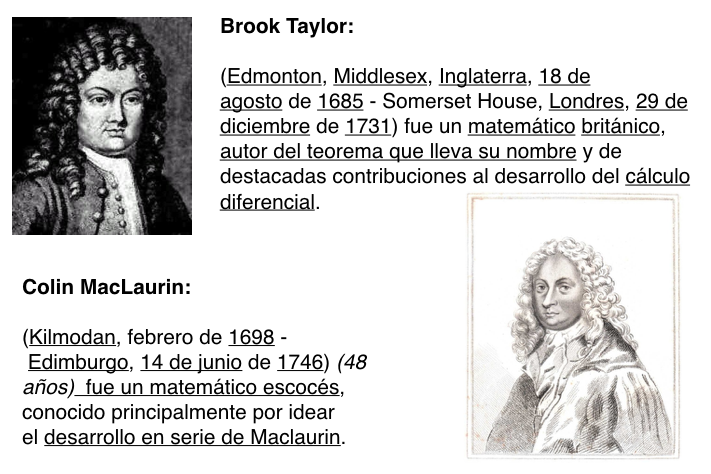
\includegraphics[width=.5\textwidth]{imagenes/Taylor/T06IM01.png}
	\end{figure}
\end{multicols}
	
	\begin{multicols}{2}
	El problema de la aproximación local de una función real de variable real $f(x)$ en un punto $a 	\in  D(f)$ consiste en hallar otra función real de variable real $g(x)$ cuyos valores se diferencien `lo menos posible' de los de $f(x)$ en un entorno de $a$, así como conocer una cota del error cometido en tal sustitución ($f$ por $g$).
	
	\begin{figure}[H]
		\centering
		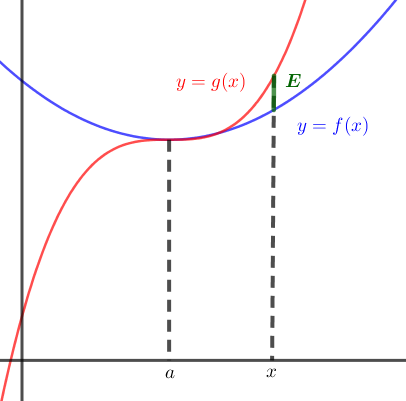
\includegraphics[width=0.25\textwidth]{imagenes/Taylor/T06IM02.png}
	\end{figure}
	
	\end{multicols}
	
	En general, las funciones $g(x)$ más sencillas que resuelven estos problemas son los polinomios \textcolor{gris}{(fáciles de calcular para cualquier valor, de derivar, de integrar, ...)} Para obtenerlas deduciremos la ``Fórmula de Taylor''.
	
	
	\begin{figure}[H]
		\centering
		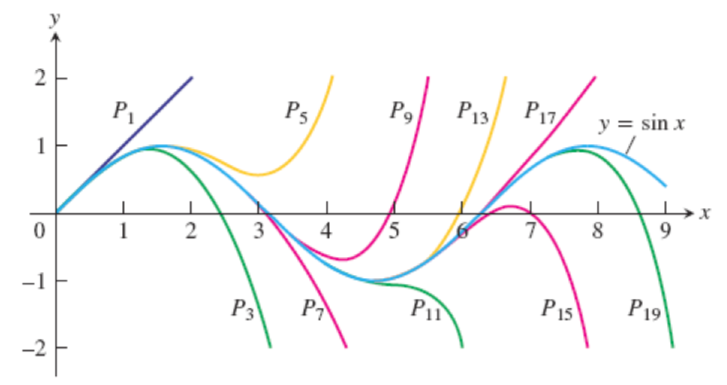
\includegraphics[width=.5\textwidth]{imagenes/Taylor/T06IM06.png}
		\caption*{Sucesivas aproximaciones de $\sin x$ con polinomios osculatrices.}
	\end{figure}

	
	\section{Fórmula de \emph{Taylor} para funciones polinómicas}
	
\begin{tikzpicture}
	\fill [left color=red!50, right color=teal!50] (0,0) rectangle (3.5,.1);
	\fill [left color=teal!50, right color=blue!50] (3.5,0) rectangle (7.5,.1);
	\end{tikzpicture}
\vspace{0.5cm}
	
	Sabemos que $\left( \mathcal{P}(x), +, \cdot\right)$, (donde  $\mathcal{P}(x)$ es el conjunto de los polinomios de una variable real) tiene estructura de `espacio vectorial'. 
	
	El conjunto $\left\{1, (x-a),(x-a)^2,(x-a)^3,\cdots \right\}$ forma una base de $\mathcal{P}(x)$, por ello, cualquier polinomio se podrá expresar de forma única en esta base:
	
	$p(x)=a_0+a_1(x-a)+a_2(x-a)^2+a_3(x-a)^3+\cdots +a_n(x-a)^n$ (*)
	
	Veamos ahora si descubrimos que relación hay entre los coeficientes del polinomio $a_i$ y las derivadas sucesivas de $p(x)$ en $x=a$:
	
	$p(x)=a_0+a_1(x-a)+a_2(x-a)^2+\cdots +a_n(x-a)^n \to p(a)=a_0$
	
	$p'(x)=a_1+2a_2(x-a)+3a_3(x-a)^2+\cdots +n a_n(x-a)^{n-1} \to p'(a)=a_1$
	
	$p''(x)=2a_2+3\cdot 2 a3 (x-a)+ \cdots + n(n-1)a_n(x-a)^{n-2} \to p''(a)=2!\; a_2$
	
	$p'''(x)=3\cdot 2 a_3+ \cdots + n(n-1)(n-2)a_n (x-a)^{n-3}\to p'''(a)=3!\; a_3$
	
	$\cdots \cdots \cdots \cdots \cdots \cdots \cdots$
	
	$p^{n)}(x)=n(n-1)(n-2)(n.3)\cdots 3\cdot 2 a_n \to p^{n)}(a)=n!\; a_n  $
	
	Llevando todos estos resultados a la expresión (*), tenemos:

\begin{cuadro-naranja}		
	\begin{equation*}
		\label{Taylor-polinomios}
		  p(x)=p(a)+\dfrac {p'(a)}{1!} (x-a)+\dfrac {p''(a)}{2!} (x-a)^2+\cdots +\dfrac {p^{n)}(a)}{n!} (x-a)^n 
	\end{equation*}
	
	\centerline{``Fórmula de Taylor para funciones polinómicas''}
	
	En el caso en que $a=0$, se obtiene la llamada ``Fórmula de MacLaurin para funciones polinómicas''.
	
	\begin{equation*}
		\label{MacLaurin-polinomios}
		 p(x)=p(0)+\dfrac {p'(0)}{1!} x+\dfrac {p''(0)}{2!} x^2+\dfrac {p'''(0)}{3!}x^3+\cdots +\dfrac {p^{n)}(0)}{n!} x^n 
	\end{equation*}
\end{cuadro-naranja}
	
	\vspace{5mm}
	\begin{miejercicio}
	.	Escribir la fórmula de Taylor de $p(x)=	4-x-2x^2+2x^3$, en el punto $a=1$
	
	\rule{200pt}{0.1pt}
	
	$p(x)=	4-x-2x^2+2x^3 \quad \to \quad p(1)=3$
	
	$p'(x)=-1-4x+6x^2 \quad \to \quad  p'(1)=1$
	
	$p''(x)= -4+12x \quad \to \quad  p''(1)=8$
	
	$p'''(x)=12 \quad \to \quad p'''(1)=12$
	
	Con esto:  $\qquad (x)=3+\dfrac {1}{1!}(x-1)+\dfrac {8}{2!}(x-1)^2+\dfrac {12}{3!}(x-1)^3$
	
	Simplificando: $\quad  p(x)= 3+(x-1)+4(x-1)^2+2(x-1)^3$
	
	\textcolor{gris}{Dejamos al lector que compruebe que se trata del mismo polinomio sin más que desarrollar las potencias de éste último.}
	\end{miejercicio}
	
	\section[Fórmula de \emph{Taylor} para funciones $f(x)$ que admiten derivadas sucesivas]{Fórmula de \emph{Taylor} para funciones $f(x)$ que admiten derivadas sucesivas\sectionmark{Fórmula de \emph{Taylor}}}
	\sectionmark{Fórmula de \emph{Taylor}}
	
\begin{tikzpicture}
	\fill [left color=red!50, right color=teal!50] (0,0) rectangle (3.5,.1);
	\fill [left color=teal!50, right color=blue!50] (3.5,0) rectangle (7.5,.1);
	\end{tikzpicture}
\vspace{0.5cm}
	
	Taylor, en el siglo $XVIII$, logró generalizar la fórmula anterior, no solo para funciones polinómicas, sino para todo tipo de funciones $f(x)$ que admitan derivadas sucesivas.
	
		\begin{multicols}{2}
		Sea $f(x)$ definida y derivable hasta orden $n$ en $[a,b]$, tal que $f^{n)}(x)$ sea ctna. en $]a,b[$. Llamaremos ``Polinomio de Taylor de grado $n$ para $f(x)$ en el punto $x=\alpha$'' \textit{(usamos $\alpha$ para diferenciarlo del extremo interior del intervalo $a$)}, a la expresión:
		
		\begin{figure}[H]
		\centering
		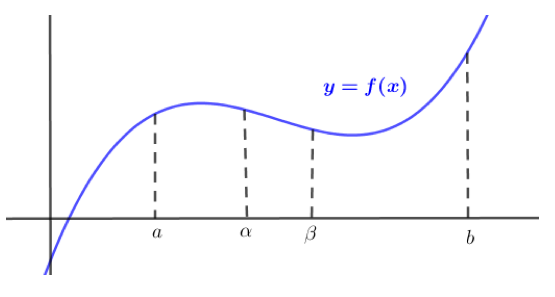
\includegraphics[width=.4\textwidth]{imagenes/Taylor/T06IM03.png}
		\end{figure}
		
		\end{multicols}

\begin{cuadro-naranja}
		
	\begin{equation*}
		\label{Taylor}
		\boxed{ \quad P_{n,f,\alpha}(x)=f(\alpha)+\dfrac {f'(\alpha)}{1!} (x-\alpha)+\dfrac {f''(\alpha)}{2!} (x-\alpha)^2+\cdots +\dfrac {f^{n)}(\alpha)}{n!} (x-\alpha)^n \quad}
	\end{equation*}
	\centerline{\emph{``Polinomio de Taylor de grado $n$ para $f(x)$ en el punto $x=\alpha$''}}
\end{cuadro-naranja}
	
	Para un punto $\beta \in [a,b]$ próximo a $\alpha$, podemos escribir:
	
	$ f(\beta)=f(\alpha)+\dfrac {f'(\alpha)}{1!} (\beta-\alpha)+\dfrac {f''(\alpha)}{2!} (\beta-\alpha)^2+\cdots +\dfrac {f^{n)}(\alpha)}{n!} (\beta-\alpha)^n \; + \; \textbf{E}$
	
	Donde $E$ mide el error cometido al sustituir $f(\beta)$ por $P_{n.f.\alpha}(\beta)$:
	
	$E=f(\beta)- \left[ f(\alpha)+\dfrac {f'(\alpha)}{1!} (\beta-\alpha)+\dfrac {f''(\alpha)}{2!} (\beta-\alpha)^2+\cdots +\dfrac {f^{n)}(\alpha)}{n!} (\beta-\alpha)^n   \right]$, que es el llamado \emph{' término complementario'} y depende de $\alpha$, $\beta$, $n$, incluso, claro está, de $f$.
	
	Supongamos $\beta$ y $n$ fijos y hagamos variar $\alpha$, con ello determinaremos $E(\alpha)$.
	
	$E'(\alpha)=\cancel{-f'(\alpha)}+\cancel{\dfrac{f'(\alpha)}{1!}}-\bcancel{\dfrac {f''(\alpha)}{1!}(\beta-\alpha)} +\bcancel{\dfrac {2f''(\alpha)}{2!}(\beta-\alpha)}-\cdots - \dfrac {f^{n+1)}(\alpha)}{n!}(\beta-\alpha)^n$
	
	
	Luego  $E'(\alpha)=-\dfrac {f^{n+1)(\alpha)}}{n!}(\beta-\alpha)^n$
	
	A partir de esta expresión podemos calcular $E(\alpha)$ aplicando el Teorema de Cauchy:
	
	\begin{equation*}
		\dfrac {E(\beta)-E(\alpha)}{\Phi(\beta)-\Phi(\alpha)}=\dfrac {E'(\theta)}{\Phi'(\theta)} \qquad \mbox{ con } \alpha<\theta<\beta
	\end{equation*}
	
	Eligiendo una función $\Phi$ que junto con $E$ cumplan las condiciones del th. de Cauchy.
	
	Como $E(\beta)=0$, elegiremos una $\Phi(x)$ que también se anule en $\beta$. Las más sencillas son: 
	
	$\Phi(x)= (\beta-x)^{n+1}; \quad \Phi(x)= (\beta-x); \quad \Phi(x)= (\beta-x)^p$
	
	Elegimos, es este caso, la primera de las opciones y aplicamos el th. de Cauchy:
	
	\begin{equation*}
		\dfrac{-E(\alpha)}{-(\beta-\alpha)^{n+1}}=\dfrac {-\dfrac {f^{n+1)}(\theta)}{(n+1)!}(\beta-\theta)^n}{-(n+1)(\beta-\theta)^n}
	\end{equation*} 
	
	
	De donde:
	
	\begin{equation*}
		E(\alpha)= \dfrac {f^{n+1)}(\theta)}{(n+1)!}\; (\beta-\alpha)^{n+1}
	\end{equation*}
	\centerline{\emph{`Forma de \textbf{LAGRANGE} del término complementario'}} 
	\vspace{1mm}
	
	
	Si hubiésemos tomado la segunda opción para $\Phi$, hubiésemos obtenido:
	
	\begin{equation*}
		E(\alpha)=\dfrac {f^{n+1)}(\theta)\; (\beta-\theta)^n}{n!}\; (\beta-\alpha)
	\end{equation*}
	\centerline{\emph{`Forma de CAUCHY del término complementario'}} 
	\vspace{1mm}
	
	Y si hubiésemos elegido la tercera opción:
	
	\begin{equation*}
		E(\alpha)=\dfrac {f^{n+1}(\theta)\; (\beta-\theta)^{n-p+1}}{n! \cdot p}\; (\beta - \alpha)^p
	\end{equation*}
	\centerline{\emph{`Forma de SCHLÖLMILCH del término complementario'}} 
	\vspace{1mm}
	
	Sustituyendo en la fórmula que proporciona $f(\beta)$ se obtiene la '' Fórmula o desarrollo de TAYLOR'' de una función $f(x)$ que admite de derivadas sucesivas. Los términos complementarios expresan el error cometido al aproximar $f(x)$ por $P_n(x)$. En general, el error es mayor cuanto menor es el grado del polinomio y cuanto más alejada esté $x$ de $\alpha$.
	
	El término complementario más usado es el de Lagrange. A estos términos complementarios también se les llama restos.
	
	Haciendo $\beta=x$:
	
	\begin{equation*}
		\label{Desarrollo-Taylor}
		\boxed{ \ \subrayado{ \ 
		\begin{split}
		\quad f(x)=\left[f(\alpha)+\dfrac {f'(\alpha)}{1!}(x-\alpha)+\dfrac {f''(\alpha)}{2!} (x-\alpha)^2 + \cdots + \dfrac {f^{n}(\alpha)}{n!} (x-\alpha)^n    \right] + \\ 
		+\boxed{\; \dfrac {f^{n+1)}(\theta)}{(n+1)!}\; (x-\alpha)^{n+1}\; } \quad \mbox{con } \alpha < \theta <x .\quad 
		\end{split}
		\ } \ }
	\end{equation*} 
	\centerline{\emph{Desarrollo de Taylor con resto de Lagrange.}} 
		
	El último término del desarrollo es el resto de Lagrange, abreviadamente podríamos escribir:  $f(x)=P_n(x)+E$
	
	Otra forma de escribir este desarrollo es haciendo $x -\alpha=h$:
	
	\begin{equation*}
		\label{Desarrollo-Taylor-h}
		\boxed{ \ \subrayado{ \ 
		\begin{split}
		\quad f(\alpha+h)=\left[f(\alpha)+\dfrac {f'(\alpha)}{1!}\; h+\dfrac {f''(\alpha)}{2!}\; h^2 + \cdots + \dfrac {f^{n}(\alpha)}{n!} \; h^n    \right]  + \\
		+\boxed{\; \dfrac {f^{n+1)}(\alpha+\theta \cdot h)}{(n+1)!}\; h^{n+1}\; } \quad \mbox{con } 0 < \theta <1 .\quad 
		\end{split} \ } \ }
	\end{equation*}
	
	Al ser $0 < \theta <1 \; $, $\; \alpha+\theta\cdot h$ es un punto intermedio del intervalo de extremos $\alpha$ y $\alpha+h$.
	
	Haciendo $\alpha=0$, tenemos el desarrollo de Maclaurin:
	
	
	\begin{equation*}
		\label{Desarrollo-Maclaurin}
		\boxed{ \ \subrayado{ \ 
		\begin{split}
		\quad f(x)=\left[f(0)+\dfrac {f'(0)}{1!}\; x+\dfrac {f''(0)}{2!}\; x^2 + \cdots + \dfrac {f^{n}(0)}{n!} \; x^n    \right]  + \\
		+\boxed{\; \dfrac {f^{n+1)}(\theta \; x)}{(n+1)!}\; x^{n+1}\; } \quad \mbox{con } 0 < \theta <1 .\quad 
		\end{split} \ } \ }
	\end{equation*}
	\centerline{\emph{Desarrollo de MacLaurin con resto de Lagrange.}}
	
	
	\section{Aproximaciones locales de algunas funciones}

\begin{tikzpicture}
	\fill [left color=red!50, right color=teal!50] (0,0) rectangle (3.5,.1);
	\fill [left color=teal!50, right color=blue!50] (3.5,0) rectangle (7.5,.1);
	\end{tikzpicture}
\vspace{0.5cm}
	
Recordando los resultados de derivadas sucesivas de las funciones elementales:
	
	\begin{miejercicio} 
	.  Desarrollo de MacLaurin de la función exponencial: $f(x)=e^x$
	
	\rule{200pt}{0.1pt}
	
	\vspace{2mm}
	
	$n=1 \to e^x=1+	\dfrac {1}{1!}x+ \boxed{\; \dfrac {e^{\theta x}}{2!}x^2}\; $
	
	$n=2 \to e^x=1+	\dfrac {1}{1!}x+ \dfrac {1}{2!}x^2+ \boxed{\; \dfrac {e^{\theta x}}{3!}x^3}\; $
	
	$n=3 \to e^x=1+	\dfrac {1}{1!}x+ \dfrac {1}{2!}x^2+ \dfrac {1}{3!}x^3+\boxed{\; \dfrac {e^{\theta x}}{4!}x^4}\; $
	
	etc $\cdots$
	
	Se dice que $P_1(x)=1+x$ es el polinomio osculatriz de primer grado de o aproximación lineal (\textit{diferencial}) de $e^x$ en el punto $0$; $P_2(x)=1+x+\frac 1 2 x^2$ es el polinomio osculatriz de segundo grado de o aproximación cuadrática  de $e^x$ en el punto $0$; $P_3(x)=1+x+\frac 1 2 x^2+ \frac 1 6 x^3$ es el polinomio osculatriz de tercer grado de o aproximación cúbica  de $e^x$ en el punto $0$;	$\cdots$
	
	Esquemáticamente:  
	\begin{equation*}\label{MacLaurin-exp}
		\boxed{\quad { e }^{ x }\; =\; \sum _{ k=1 }^{ n }{ \dfrac { 1 }{ k! } \; { x }^{ k } } 	\quad +\quad \dfrac { { e }^{ \theta x } }{ (k+1)! } { x }^{ k+1 } \quad}  
	\end{equation*}
	\centerline{\emph{Desarrollo de MacLaurin de $e^x$.}}
	
	\vspace{5mm} Como ejercicio, vamos a calcular con aproximación lineal, cuadrática y cúbica, el valor aproximado que da el desarrollo para $e^{0.4}$, así como intentar acotar los errores cometidos.
	
	\vspace{2mm}
	
	\begin{multicols}{2}
	$\triangleright \ \   n=1 \to e^{0.4}=1+0.4=1.4 $. Aproximación lineal.
	
	$E=\dfrac {e^{\theta x}}{2!}\; (0.4)^2 < \dfrac {e^1}{2}\; 0,16 < \dfrac {3}{2} \cdot (0.16)=0.24 \qquad 0<\theta x< 0,4$
	
	\vspace{2mm}
	
	$\triangleright \ \ n=2 \to e^{0.4}=1+0.4+\frac 1 2\;  0.4^2=1.48 $. Aproximación cuadrática.
	
	$E=\dfrac {e^{\theta x}}{3!}\; (0.4)^3 < \dfrac {e^1}{6}\; 0,064 < \dfrac {3}{6} \cdot (0.064)=0.24 \qquad 0<\theta x< 0,032$
	


	$\quad$
	
	$\triangleright \ \ n=3 \to e^{0.4}=1+0.4+\frac 1 2 \; 0.4^2+ \frac 1 {6}\; 0.4^3 =1.490666\cdots $. Aproximación cúbica.
	
	$E=\dfrac {e^{\theta x}}{4!}\; (0.4)^4 < \dfrac {e^1}{24}\; 0,0256 < \dfrac {3}{24} \cdot (0.0256)=0.24 \qquad 0<\theta x< 0,0032$
	
	
	
	Mostramos una figura que represente $e^x$ y las sucesivas aproximaciones $ P_1; P_2; P_3$
	
	\begin{figure}[H]
	\centering
		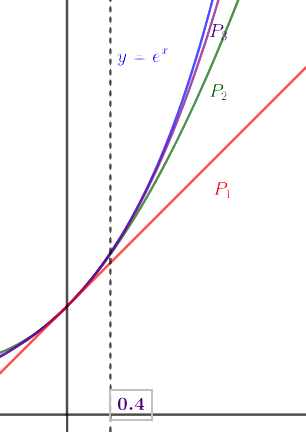
\includegraphics[width=.25\textwidth]{imagenes/Taylor/T06IM04.png}
		\end{figure}
	
	\end{multicols}
	
	\end{miejercicio}
	 	 
\begin{miejercicio}  
.  Desarrollo de MacLaurin de la función seno: $\quad f(x)=\sin x$

\rule{200pt}{0.1pt}
	 
	Suponemos conocido que $\ \sin^{n)}(x)=\sin (x+n\frac \pi 2)$
	 
	 En $x=0$, para $n=0\to \sin 0=0; \quad n=1\to \sin (\pi/2)=1; \quad n=2\to \sin (2\pi/2)=\sin (\pi)=0; \quad n=3 \to \sin (3\pi/2)=-1; \quad \cdots $. Solo quedan las derivadas impares.
	 
	 El desarrollo de MacLaurin, hasta orden 6 (desarrollar hasta orden 5 es tontería, ya que el término de orden 6 es par, cero; de este modo, el error cometido se medirá con el término séptimo y nos dará más precisión). ¡OJO, $x$ en radianes!
	 
	\vspace{2mm} $\sin x= \dfrac {1}{1!}x-\dfrac {1}{3!}x^3+\dfrac {1}{5!}x^5 +\dfrac {\sin \theta x}{7!}x^7; \quad 0<\theta <x$
	 
	 
	\vspace{2mm} Calculemos una aproximación de quinto grado del $\sin(0.2)$, así como una cota del error cometido:
	  $\quad \sin 0.2= \dfrac {1}{1!}0.2-\dfrac {1}{3!}0.2^3+\dfrac {1}{5!}0.2^5=1.988669333\cdots$

	  Acotemos el error: $|E|=\left| \dfrac {\sin (\theta x)}{7!} \right|\; 0.2^7 < \; [\; \sin (\theta x) < 1 \;] < 0,000000002539683 < 0,0000000026 $
	  
	  Adjuntamos una imagen al ejemplo.
	 
	 
	\begin{figure}[H]
	\centering
		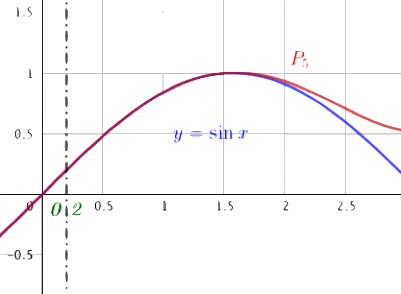
\includegraphics[width=.5\textwidth]{imagenes/Taylor/T06IM05.png}
	\end{figure}
	
	
	El desarrollo completo de la función $\sin x$ es:
	
	$\sin x \approx x-\dfrac{x^3}{3!}+\dfrac{x^5}{5!}-\dfrac{x^7}{7!}+\cdots$. Escrito más brevemente e incluyendo el resto de Lagrange:
	
	\begin{equation*}\label{MacLaurin-exp}
		\boxed{\quad \sin x \; =\; \sum _{ k=1 }^{ n }{ \dfrac {(-1)^k}{(2k+1)!}\;x^{2k+1}  +\dfrac {(1)^{2k+3}}{(2k+3)!} \; x^{2k+3}\quad}}  
	\end{equation*}
	\centerline{\emph{Desarrollo de MacLaurin de $\sin x$.}}
	
\end{miejercicio}

\vspace{5mm}	
\begin{miejercicio}
	
Desarrollo de Taylor para de la función logarítmica  $f(x)=\mathrm{ln}\;x$, en un entorno de $\alpha=e$:

\rule{200pt}{0.1pt}
	
	\vspace{3mm} $\mathrm{ln}\; x = 1 + \dfrac 1 1 \dfrac 1 e (x-e) +- \dfrac 1 2 \dfrac 1 {e^2} (x-e)^2 + \cdots + \dfrac {(-1)^{n-1}}{n} \dfrac 1 {e^n} (x-e)^n + $
	
	$ \qquad \ \ + \dfrac {(-1)^n}{n+1} \dfrac 1 {\theta ^{n+1}} (x-e)^{n+1} \, ; \ \qquad e < \theta < x \quad \vee \quad 0 < x < \theta < e$
	
	\vspace{3mm} Como aplicación, calcularemos un polinomio de tercer grado osculatriz para aproximar $\mathrm{ln}\; 3$ y una cota del error cometido.
	
	\vspace{2mm} $\mathrm{ln}\; 3 = 1+ \frac 1 e 3-e)- \frac 1 {2e^2}(3-x)^2+ \frac 1 {3e^3}(3-e=^3 = 1.09861$
	
	$|E|=|\; - \frac 1 4 \frac 1 {\theta^4} (3-e)^4  \;| < 0.00004; \quad (e<\theta<3) \;$
		
\end{miejercicio}

\vspace{5mm}	
	
	
\subsection{Aplicaciones de la fórmula de Taylor al cálculo de límites}

\begin{tikzpicture}
	\fill [left color=red!50, right color=teal!50] (0,0) rectangle (3.5,.01);
	\fill [left color=teal!50, right color=blue!50] (3.5,0) rectangle (7.5,.01);
	\end{tikzpicture}
\vspace{0.5cm}

	Si es posible, se puede sustituir cada expresión del límite se desea calcular por el desarrollo adecuado de Taylor, aí, el problema del cálculo de límites se reduce al problema del cálculo de límites de funciones polinómicas.

\vspace{5mm}	
\begin{miejercicio}
	.  Calcula $\quad \underset{x\to 0}{lim}\;{\dfrac {\tan 2x - 2 \tan x}{x \; \tan x \; \tan 2x}}$	
	
	\rule{200pt}{0.1pt}
	
	Como
	$ \ \ \tan x=x+x^3/3+ \cdots$
	$\quad\to \quad \tan 2x = 2x + (2x)^3/3 + \cdots = 2x + \frac 8 3 x^3 + \cdots $
	
	Sustituyendo:
	$\ \underset{x\to 0}{lim}\;{\dfrac {\tan 2x - 2 \tan x}{x \; \tan x \; \tan 2x}}= \underset{x\to 0}{lim}\; { \dfrac {  (2x + \frac 8 3 x^3 + \cdots ) - 2\; (x+x^3/3+ \cdots) }  {  x\cdot (x+x^3/3+ \cdots) \cdot(2x + \frac 8 3 x^3 + \cdots )   }    } =$
	
	$ = \underset{x\to 0}{lim}\;{\dfrac {2x^3+\cdots}{2x^3+\cdots}}=1$ 
	
	$\quad$
	
	Compare el/la lector/a la rapidez del cálculo por este método o aplicando la regla de L'Hôpital.

\end{miejercicio}

\vspace{5mm}
\begin{miejercicio} 
.  Calcula $\underset{x\to 0}{lim}\;{\dfrac {\tan x \; \arctan x- x^2}{x^6}}$

\rule{200pt}{0.1pt}

	Se necesita derivar al menos 5 veces (L'H) numerador y denominador para resolver el límite.
	Si sustituimos las expresiones por los desarrollos de MacLaurin correspondientes y hacemos cuatro operaciones con los polinomios, tendremos:
	
	\vspace{2mm} $\underset{x\to 0}{lim}\;{\dfrac {\tan x \; \arctan x- x^2}{x^6}}= \underset{x\to 0}{lim}{\dfrac {\frac 2 9 \; x^6 + \cdots }{x^6}}\;=2/9$
\end{miejercicio}

\vspace{5mm}
\begin{miejercicio} 
.  Calcula $\quad \underset{x\to 0}{lim}\;{\dfrac {(\cos x -1)(\mathrm{ln}((1+x)-x)-\frac 1 4 x^4}{x^5}}$

\rule{200pt}{0.1pt}

$\underset{x\to 0}{lim}\;{\dfrac {(\cos x -1)(\mathrm{ln}((1+x)-x)-\frac 1 4 x^4}{x^5}} = -1/6$
		
\end{miejercicio}

\vspace{5mm}
\begin{miejercicio}
	
  Sea $f(x)=e^{2x}$. En contrar el órden $n$ del polinomio de Taylor de$f$ en $x_0=0$ (MacLaurin) tal que al aproximar $f(1)=e^2$ por el $P_n$ encontrado, el error sea menor que $\frac 1 {1000}$ (una milésima).
		
\rule{200pt}{0.1pt}	
		
		$f'(x)=2e^{2x}; \; f''(x)=2^2 e^{2x}; \; f'''(x)=2^3 e^{2x}; \cdots ; \; f^{n)}(x)=2^n e^{2x}$
		
		Por ello:
		$\ \ f(0)=1; \; f'(0)=2; \; f''(2)=2^2; \; f'''(2)=2^3; \cdots ; \; f^{n)}(0)=2^n$
		
		El polinomio de MacLaurin de orden $n$ es:
		
		$P_n(x)=1+ 2x+\dfrac{4}{2}x^2+\dfrac{8}{6}x^3+ \cdots + \dfrac{2^n}{n!}x^n$
		
		Vamos a por el resto de Lagrange:
		$ \quad E_n(x)=\dfrac{2^{n+1}\; e^{2\theta}}{(n+1)!}\; x^{n+1}$
		
		\vspace{2mm} Como $\theta\in]0,x[$, con $x>0$, tenemos: (queremos calcular $f(1); \quad \theta=1$)
		
		
		\vspace{2mm} $E_n(1)=\dfrac{2^{n+1}\; e^{2 \theta}}{(n+1)!}\; 1^{n+1} < 
		\dfrac{2^{n+1}\; e^{2\cdot 1}}{(n+1)!}\; 1^{n+1} <
		 \dfrac{2^{n+1}\; 3^{2}}{(n+1)!} < \dfrac {18\cdot 2^n}{(n+1)!} < \dfrac {1}{100}  $
		
		
		\vspace{2mm} La última ecuación $\dfrac {18\cdot 2^n}{(n+1)!} < \dfrac {1}{100}  $, que nos sirve para determinar el grado $n$ que hemos de tomar para aproximar $f(1)$ por $P_n(1)$ solo puede ser resuelta por `tanteo'. Probando, encontramos:
		
		\vspace{2mm} $E_{10}(1)<\dfrac {2^{10+1}3^2}{(10+1)!}=\dfrac {8}{17325}\approx 0.00046\cdots < \dfrac {1}{1000}$
		
		\vspace{2mm} Puede el lector calcular $P_{10}(1)$ y comparar (con una calculadora) con el valor de f(1) para comprobar que el error que se comete es, efectivamente, menor que una milésima.
\end{miejercicio}

\vspace{5mm}
\begin{miejercicio}
	
Probar que $\quad \forall \; x \; \in \; \mathbb{R}\; : \quad e^x \; \ge \; 1 + x$

\rule{200pt}{0.1pt}	

Acudiendo al desarrollo es serie de MacLaurin de la función $e^x$:
		
\vspace{2mm} $e^x=1+x+E\ge 1+x \qquad \mbox{ al ser } \quad E=\dfrac {e^c}{2!}x^2\ge 0$
\end{miejercicio}

\vspace{1cm}

\color{black}





\begin{comment}

%%%%%%%%%%%%%%%%%%%%%%%%%%%%%%%%%%%. SECCIONES
\chapter{texto}
\begin{tikzpicture}
	\fill [left color=red!50, right color=teal!50] (0,0) rectangle (6.5,.2);
	\fill [left color=teal!50, right color=blue!50] (6.5,0) rectangle (11.5,.2);
	\end{tikzpicture}

\vspace{1cm}
\section{texto}
\begin{tikzpicture}
	\fill [left color=red!50, right color=teal!50] (0,0) rectangle (3.5,.1);
	\fill [left color=teal!50, right color=blue!50] (3.5,0) rectangle (7.5,.1);
	\end{tikzpicture}
\vspace{0.5cm}

\subsection{texto}
\begin{tikzpicture}
	\fill [left color=red!50, right color=teal!50] (0,0) rectangle (3.5,.01);
	\fill [left color=teal!50, right color=blue!50] (3.5,0) rectangle (7.5,.01);
	\end{tikzpicture}
\vspace{0.5cm}


%%%%%%%%%%%%%%%%%%%%%%%%%%%%%%%%%%%. \begin{ ------>. 
detsacado;  cuadro-naranja;  cuadro-gris;  miejercicio (solución extensa);  mipropuesto (solución corta y fuera del cuadro)

%%%%%%%%%%%%%%%%%%%%%%%%%%%%%%%%%%%. CURIOSIDAD
\vspace{1cm}
\color{ForestGreen!80}
\rule{250pt}{0.2pt}
Texto
\vspace{-8mm}
\begin{flushright}
\rule{250pt}{0.2pt}		
\end{flushright}	
\color{black}
\end{comment}

 %Taylor
\chapter{Introducción a las ecuaciones diferenciales}
\setlength{\parindent}{0cm}

\begin{tikzpicture}
	\fill [left color=red!50, right color=teal!50] (0,0) rectangle (6.5,.2);
	\fill [left color=teal!50, right color=blue!50] (6.5,0) rectangle (11.5,.2);
	\end{tikzpicture}
\begin{comment}
\vspace{1cm}
\section{Uno.Uno}
\begin{tikzpicture}
	\fill [left color=red!50, right color=teal!50] (0,0) rectangle (3.5,.1);
	\fill [left color=teal!50, right color=blue!50] (3.5,0) rectangle (7.5,.1);
	\end{tikzpicture}
\vspace{0.5cm}

\vspace{1cm}
\subsection{Uno.Uno.Uno}
\begin{tikzpicture}
	\fill [left color=red!50, right color=teal!50] (0,0) rectangle (3.5,.01);
	\fill [left color=teal!50, right color=blue!50] (3.5,0) rectangle (7.5,.01);
	\end{tikzpicture}
\vspace{0.5cm}

\end{comment}

\section{Ecuaciones diferenciales}
\begin{tikzpicture}
	\fill [left color=red!50, right color=teal!50] (0,0) rectangle (3.5,.1);
	\fill [left color=teal!50, right color=blue!50] (3.5,0) rectangle (7.5,.1);
	\end{tikzpicture}
\vspace{0.5cm}

Las leyes físicas se expresan habitualmente mediante relaciones entre magnitudes y sus derivadas, esto es lo que se conoce como \textbf{ecuaciones diferenciales}. 

Por ejemplo, una partícula libre en un campo gravitatorio evoluciona de modo que $\displaystyle m\, \dv[2]{x}{t}=-g\, (cte)$, un oscilador armónico (muelle) lo hace en la forma $\displaystyle m\, \dv[2]{x}{t}=-kx$, número de átomos en una desintegración radiactiva, es proporcional a la cantidad de átomos en ese instante $\displaystyle \dv{N}{t}=-kN$, etc.

Existen multitud de técnicas para resolver este tipo de ecuaciones, incluyendo soluciones numéricas que se obtienen con ordenador.



Una ecuación diferencial es una ecuación matemática que relaciona una función con sus derivadas. En las matemáticas aplicadas, las funciones usualmente representan cantidades físicas, las derivadas representan sus razones de cambio, y la ecuación define la relación entre ellas. Como estas relaciones son muy comunes, las ecuaciones diferenciales juegan un rol primordial en diversas disciplinas, incluyendo la física, la ingeniería, la química, la economía, y la biología.

En las matemáticas puras, las ecuaciones diferenciales se estudian desde perspectivas diferentes, la mayoría concernientes al conjunto de las soluciones de las funciones que satisfacen la ecuación. Solo las ecuaciones diferenciales más simples se pueden resolver mediante fórmulas explícitas; sin embargo, se pueden determinar algunas propiedades de las soluciones de una cierta ecuación diferencial sin hallar su forma exacta. Si la solución exacta no puede hallarse, esta puede obtenerse numéricamente, mediante una aproximación usando ordenadores. 

Las ecuaciones diferenciales pueden dividirse en varios tipos. Aparte de describir las propiedades de la ecuación en si, las clases de las ecuaciones diferenciales pueden ayudar a buscar la elección de la aproximación a una solución. Es muy común que estas distinciones incluyan si la ecuación es: Ordinaria/Derivadas Parciales, Lineal/No lineal, y Homogénea/Inhomogénea. Esta lista es demasiado grande; hay muchas otras propiedades y subclases de ecuaciones diferenciales las cuales pueden ser muy útiles en contextos específicos.

Una ecuación diferencial ordinaria (EDO) es una ecuación que contiene una función de una variable independiente y sus derivadas. El término ``ordinaria'' se usa en contraste con la ecuación en derivadas parciales (`concepto que no hemos estudiado porque forma parte del cálculo con funciones de varias variables') la cual puede ser respecto a más de una variable independiente.

Las ecuaciones diferenciales lineales, las cuales tienen soluciones que pueden sumarse y ser multiplicadas por coeficientes, están bien definidas y comprendidas, y tienen soluciones exactas que pueden hallarse. En contraste, las EDOs cuyas soluciones no pueden sumarse son no lineales, y su solución es más intrincada, y muy pocas veces pueden hallarse en forma exacta de funciones elementales: las soluciones suelen obtenerse en forma de series o forma integral. Los métodos numéricos y gráficos para EDOs, pueden realizarse manualmente o mediante ordenadores, se pueden aproximar las soluciones de las EDOs y su resultado puede ser muy útil, muchas veces suficientes como para prescindir de la solución exacta y analítica.


\vspace{7mm}

\vspace{1cm}
\color{ForestGreen!80}
\rule{250pt}{0.2pt}

APLICACIONES:

\vspace{3mm}

\normalsize{El} estudio de ecuaciones diferenciales es un campo extenso en matemáticas puras y aplicadas, en física y en la ingeniería. Todas estas disciplinas se interesan en las propiedades de ecuaciones diferenciales de varios tipos. 

Las matemáticas puras se focalizan en la existencia y unicidad de las soluciones, mientras que las matemáticas aplicadas enfatizan la justificación rigurosa de los métodos de aproximación de las soluciones. Las ecuaciones diferenciales juegan un rol muy importante en el modelado virtual de cualquier proceso físico, técnico, o biológico, por ejemplo, tanto el movimiento celeste, como el diseño de un puente, o la interacción entre neuronas. Las ecuaciones diferenciales que se plantean para resolver problemas de la vida real, no necesariamente son resolubles directamente, es decir, sus soluciones no tienen una expresión en forma cerrada. Cuando sucede esto, las soluciones se pueden aproximar usando métodos numéricos.

Muchas leyes de la física y la química se formalizan con ecuaciones diferenciales. 

En biología y economía, las ecuaciones diferenciales se utilizan para el modelado del comportamiento de sistemas complejos. 

La teoría matemática de las ecuaciones diferenciales se desarrolló inicialmente con las ciencias donde las ecuaciones se originaban y donde se encontraban resultados para las aplicaciones. Sin embargo, algunas veces se originaban problemas diversos en campos científicos distintos, de los cuales resultaban ecuaciones diferenciales idénticas. Esto sucedía porque, detrás de la teoría matemática de las ecuaciones, puede verse un principio unificado detrás de los fenómenos. Como por ejemplo, si se considera la propagación de la luz y el sonido en la atmósfera, y de las ondas sobre la superficie de un estanque. Todos estos fenómenos pueden describirse con la misma ecuación en derivadas parciales de segundo orden, `la ecuación de onda', la cual nos permite pensar a la luz y al sonido como formas de onda, y en forma similar a las ondas en el agua. 

La conducción de calor, la teoría que fue desarrollada por Joseph Fourier, está gobernada por otra ecuación en derivadas parciales de segundo orden, `la ecuación de calor'. Resulta que muchos procesos de difusión, aunque aparentan ser diferentes, están descritos por la misma ecuación. 

\footnotesize{En física, las ecuaciones de campo de Einstein (conocidas como EFE, por Einstein Field Equations) son un conjunto de diez ecuaciones diferenciales de segundo grado en derivadas parciales de la tepría de la relatividad general de Albert Einstein que describen la interacción fundamental de la gravitación como resultado de que el espacio-tiempo está siendo curvado por la materia y ya energía. En el límite clásico no-relativista, esto es, a velocidades pequeñas  comparadas con la luz y campos gravitacionales relativamente débiles, las ecuaciones de campo de Einstein se reducen a la ecuación de Poisson para el campo gravitatorio, que es equivalente a la ley de gravitación de Newton}\normalsize{.}

\footnotesize{\rightline{Fuente: Wikipedia}}\normalsize{.}

\vspace{-8mm}
\begin{flushright}
\rule{250pt}{0.2pt}		
\end{flushright}	
\color{black}

	%\begin{figure}[H]
 	%\centering
	%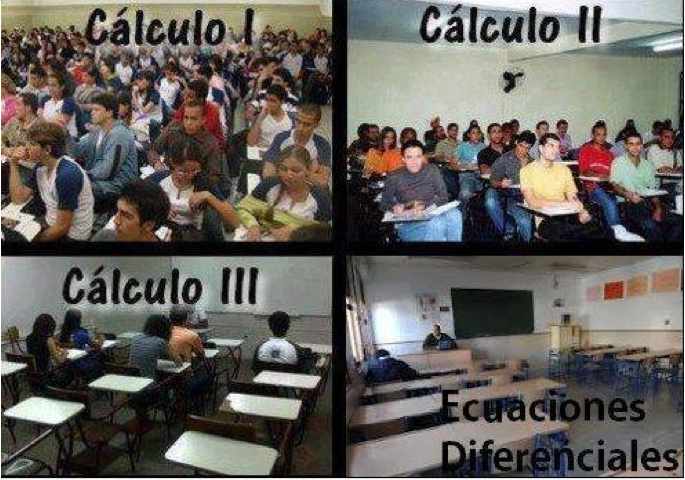
\includegraphics[width=1\textwidth]{imagenes/imagenesEDO/T09IM01.png}
	%\end{figure}


\section{Ecuaciones diferenciales ordinarias}
\begin{tikzpicture}
	\fill [left color=red!50, right color=teal!50] (0,0) rectangle (3.5,.1);
	\fill [left color=teal!50, right color=blue!50] (3.5,0) rectangle (7.5,.1);
	\end{tikzpicture}
	
	Sea $y=f(x)$, vamos a estudiar las ecuaciones donde intervienen la variable $x$, la función $y\;$ y alguna de sus derivadas $y';\; y''; \; y'''; \; \cdots$. 
	
	Ejemplos de este tipo de ecuaciones son:
	$\quad xy'= y\; ; \qquad y''=y\; y'\; ; \qquad (y'')^2=\dfrac {x+y'}{1+x^2}$

\begin{cuadro-naranja}
	
\begin{defi}
Llamamos Ecuación Diferencial Ordinaria (EDO) a una ecuación el que intervengan la variable independiente $x$, una función $y(x)$ y una o varias derivadas de $y(x)$.	
\end{defi}
\end{cuadro-naranja}

\begin{cuadro-naranja}
	
\begin{defi}
Llamamos `orden' de una EDO al orden de la mayor derivada que interviene en la ecuación. 
\end{defi}
\end{cuadro-naranja}

\begin{cuadro-gris}


Ejemplos: $\quad 2x+y\; y'=0 \text{ (orden 1) }\; ; \quad x^2 \dfrac {\dd^3 y}{\dd x^3}- \left( \dfrac {\dd y}{\dd x} \right)^4=1 \text{ (orden 3) }\; $

$ \dfrac {\dd^2 y}{\dd x^2}\; \cos x + \cos y =0 \text{ (orden 2) } $
\end{cuadro-gris}

Además,

\begin{cuadro-naranja}
	
\begin{defi}
Una EDO de orden `$n$' es `lineal' si se puede escribir en la forma:

\begin{equation}
	a_n(x)\; \dfrac {\dd^n y}{\dd x^n}+a_{n-1}(x)\; \dfrac {\dd^{n-1} y}{\dd x^{n-1}}+ \cdots + a_1(x)\;  \dfrac {\dd y}{\dd x}+a_0(x)\; y=b(x)
\end{equation}	
donde $a_i$ y $b$ solo dependen de $x$
\end{defi}
\end{cuadro-naranja}

\begin{cuadro-gris}

Ejemplos de EDO lineales:

$\sin x \; y''+y=e^x\; ; \quad \dfrac {1}{1+x^2}\; y'''+ (x^4-1)\; y=0\; ; \quad x\; \dfrac {\dd^4 y}{\dd x^4}+ x^2 \; \dfrac {\dd^2 y}{\dd x^2}+x^4\; y = x$

En cambio, no son EDO lineales:

$y\; y'=1;\qquad  \left( \dfrac{\dd y}{\dd x} \right)^2+y=0; \qquad \cos x\; \dfrac {\dd y}{\dd x}+\mathrm{ln} y=x\; \cos y$
	
\end{cuadro-gris}

\begin{cuadro-naranja}

\begin{defi}
Dada una EDO de orden $n$, llamamos `solución'	de la EDO a una función $y=f(x)$ definida en un intervalo $I$, de forma que cuando sustituimos $y=f(x)$ y sus derivadas en la EDO, ésta se verifica en todo $I$.
\end{defi}
\end{cuadro-naranja}

\begin{cuadro-gris}
\begin{ejem}
Consideremos la EDO $\quad y'+xy=x\; $	. Es fácil comprobar que la función $y=f(x)=1+e^{-{x^2}/2}\; $ es solución de esta EDO en todo $\mathbb R$, pero, la función $y=g(x)=1+k\cdot e^{-{x^2}/2}\; \; \text{ con } k\in \mathbb R \; $ también lo es.. Es decir, esta EDO tiene infinitas soluciones en $\mathbb R$.

Se recomienda al lector que compruebe lo dicho anteriormente.
\end{ejem}
\end{cuadro-gris}

\begin{cuadro-gris}
\begin{ejem}
Para la EDO $\; y''+y=0\; $, las funciones $y=\sin x$ e $y=\cos x$ son soluciones en todo $\mathbb R$. Y, en general, dadas dos constantes $c_1, c_2 \in \mathbb R$, la función $y=c_1\; \sin x + c_2 \; \cos x$ también es solución en todo $\mathbb R$.

Se recomienda al lector que compruebe lo dicho anteriormente.
\end{ejem}
\end{cuadro-gris}

\begin{cuadro-gris}
\begin{ejem}
Para la EDO $\; y'\; y^2=0 \;$	, la función $y=\dfrac 1 x$ es solución, pero en $\mathbb R^+$

Se recomienda al lector que compruebe lo dicho anteriormente.
\end{ejem}
\end{cuadro-gris}

Con los ejemplos vistos anteriormente, el conjunto de todas las soluciones de una EDO puede ser infinito. En ocasiones, nos interesa conocer solamente alguna de esas soluciones y no todas, por lo que se prefijan algunas condiciones previas a la solución buscada:

\begin{cuadro-naranja}

\begin{defi}{Problema de los Valores Iniciales.}

Dada una EDO de orden $n$ en un intervalo $I$ y un punto $x_0\in I$, llamamos `problema de los valores iniciales' (PVI, en lo que sigue) al problema de encontrar las soluciones de la EDO en $I$ y que además satisfagan las condiciones iniciales impuestas de antemano:

\begin{equation*}
	y(x_0)=c_0; \; y'(x_0)=c_1; \; y''(x_0)=c_2; \; \cdots ; \; y^{n-1}(x_0)=c_{n-1}
\end{equation*}

donde los $c_i$ son números prefijados.
\end{defi}
\end{cuadro-naranja}

\begin{cuadro-naranja}
\begin{ejem}.

--- El problema PVI $\; \begin{cases} 2y\; y'=e^x \\ y(0)=0 \end{cases}\; $. Tiene como solución la función $y=e^{x/2}\; $. Puede comprobarse que es la única solución que admite el problema.

--- El problema PVI $\; \begin{cases} 2y\; y'=e^x \\ y(0)=-1 \end{cases}\; $, tiene como única solución $y=-e^{x/2}$. Compruébese.

--- La EDO de segundo orden $y''-y=x$ tiene por soluciones todas las funciones de la forma $y=-x+c_1 e^x+c_2 e^{-x} \; \forall c_1, c_2 \in \mathbb R \; $, Así, el PVI dado por $\; \begin{cases} 2y \; y'=e^x \\ y(1)=0; \; y'(1)=0 \end{cases}\; $, tiene como íunica solución $y=-x+e^{x-1}$. Compruébese.

Aunque en los ejemplos anteriores los PVI tienen solución única, pude haber problemas PVI en que hayan más de una solución.
\end{ejem}
\end{cuadro-naranja}

\vspace{5mm}
\section{Modelos matemáticos de problemas de ciencia}
\begin{tikzpicture}
	\fill [left color=red!50, right color=teal!50] (0,0) rectangle (3.5,.1);
	\fill [left color=teal!50, right color=blue!50] (3.5,0) rectangle (7.5,.1);
	\end{tikzpicture}

\begin{small}
En muchas ocasiones es deseable describir en términos matemáticos el comportamiento de algunos sistemas o fenómenos de la vida real, tanto de tipo físico, químico, sociológico, económico... La descripción matemática de un sistema de fenómenos se llama `modelo matemático' y se construye con ciertos objetivos, como el de entender que ocurrirá en el futuro o que ocurrió en el pasado. Por ejemplo, podemos desear entender los mecanismos de cierto ecosistema al estudiar el crecimiento de la población animal en ese sistema, o podemos desear datar fósiles y analizar el decaimiento de una sustancia radiactiva ya sea en el fósil o en el estrato en que éste fue descubierto. 

Para la realización de un modelo matemático sobre un sistema, primero hay que identificar todas las variables que ocasionan que el sistema cambie y posteriormente establecer de qué manera estas variables afectan al sistema. Es claro que cuantas más variables que afectan al sistema se añadan mejor resolución tendrá el modelo que se obtenga. Sin embargo, el modelo será cada vez más complejo cuantas más variables entren en juego. Por ello, a veces un modelo de baja resolución (es decir, con pocas variables) es suficiente para determinar de forma aproximada la solución de nuestro problema. 

A continuación estudiaremos algunos modelos matemáticos clásicos en diferentes áreas de las Ciencias.

\subsection{Dinámica poblacional}
\begin{tikzpicture}
	\fill [left color=red!50, right color=teal!50] (0,0) rectangle (3.5,.01);
	\fill [left color=teal!50, right color=blue!50] (3.5,0) rectangle (7.5,.01);
	\end{tikzpicture}
	
El economista Thomas Malthus hizo uno de los primeros intentos para modelar el crecimiento de una población. Así, supuso que la razón de la población en un cierto tiempo $t$ es proporcional a la población total en ese tiempo. Es decir, si llamamos $P(t)$ a la población en el tiempo $t$ entonces se obtiene que 

\begin{equation*}
	\dfrac {\dd P}{\dd t}=k\; P\; ,
\end{equation*}

donde $k$ es una constante que depende de la población estudiada.

Aunque este modelo es de baja resolución, aún así sigue siendo útil para el estudio de algunas poblaciones a tiempo corto, como, por ejemplo, poblaciones de cultivos de bacterias. 


\subsection{Decaimiento radiactivo}    
\begin{tikzpicture}
	\fill [left color=red!50, right color=teal!50] (0,0) rectangle (3.5,.01);
	\fill [left color=teal!50, right color=blue!50] (3.5,0) rectangle (7.5,.01);
	\end{tikzpicture}

El núcleo de algunos átomos están formados por combinaciones de protones y neutrones inestables, es decir, los átomos se desintegran o se convierten en átomos de otras sustancias. En estos casos se dice que los núcleos son radiactivos. Por ejemplo, el radio $^{ 226 }{ Ra }$, intensamente radiactivo, se transforma en gas radón $^{ 222 }{ Rn }$.
 
Para modelar el fenómeno de decaimiento radiactivo, dada una cantidad $A(t)$ de una sustancia en el tiempo $t$, se supone que la razón con la que los núcleos se desintegran es proporcional a la cantidad existente, esto es, 
\begin{equation*}
	\dfrac {\dd A}{\dd t}= k\; A\; ,
\end{equation*}

con $k$ una constante que depende de la sustancia estudiada. 

\subsection{Ley de calentamiento-enfriamiento de Newton}
\begin{tikzpicture}
	\fill [left color=red!50, right color=teal!50] (0,0) rectangle (3.5,.01);
	\fill [left color=teal!50, right color=blue!50] (3.5,0) rectangle (7.5,.01);
	\end{tikzpicture}
	  
La ley empírica de enfriamiento/calentamiento de Newton establece que la rapidez con la que cambia la temperatura de un cuerpo es proporcional a la diferencia entre la temperatura del cuerpo y la del medio que lo rodea (la temperatura ambiente). 
 
Si denotamos por $T(t)$ a la temperatura del cuerpo en el tiempo $t$ y $T_a$ a la temperatura del ambiente, entonces, la ley de enfriamiento/calentamiento de Newton determina que 
  
  \begin{equation*}
  	\dfrac {\dd T}{\dd t}= k\; \left( T(t)-T_a \right)\; ,
  \end{equation*}
  
donde k es la constante de proporcionalidad. 

\subsection{Reacciones químicas} 
 \begin{tikzpicture}
	\fill [left color=red!50, right color=teal!50] (0,0) rectangle (3.5,.01);
	\fill [left color=teal!50, right color=blue!50] (3.5,0) rectangle (7.5,.01);
	\end{tikzpicture}
	 
En algunas reacciones químicas la rapidez con la que las moléculas de una sustancia $A$ se descomponen es proporcional a la cantidad de sustancia que queda sin reaccionar. Así, si llamamos $c(t)$ a la cantidad de la sustancia $A$ en el tiempo $t$ entonces 
  
 \begin{equation*}
 	\dfrac {\dd c(t)}{\dd t}= k\;( A\;- \; c(t)) ,
 \end{equation*} 
    
donde k es una constante (dependiente de la sustancia A).
  
   
Un ejemplo de este tipo, llamada reacción de primer orden, está dada por la conversión del cloruro de terbutilo $(CH_3)_3CCl$ en alcohol t-butílico $(CH_3)_3COH$: 
   
\begin{equation*}
	(CH_3)_3CCl \; + \; NaOH \longrightarrow (CH_3)_3COH\; + \; NaCl
\end{equation*}
   
   Solo la concentración de cloruro de terbutilo controla la rapidez de la reacción. 
   
   Sin embargo, en la reacción 
   
   \begin{equation*}
   	CH_3Cl + NaOH \longrightarrow  CH_3OH + NaCl \; ,
   \end{equation*}
   
la razón con la que avanza la reacción es proporcional al producto de las concentraciones de cloruro de metilo $CH_3Cl$ y de hidróxido de sodio $NaCl$ que quedan. 
   
   Para describir en general una reacción de este tipo, conocida como reacción de segundo orden, supongamos que se combina una molécula de una sustancia $A$ con una molécula de una sustancia $B$ para formar una molécula de una sustancia $C$ (más otras sustancias). Si $c(t)$ denota la cantidad de la sustancia $C$ que se ha formado en el tiempo $t$ y si $a_0,\; b_0$ son, respectivamente, las cantidades de las sustancias $A$ y $B$ en el momento inicial $t = 0$, entonces las cantidades de $A$ y $B$ en tiempo $t$ son $a_0- c(t)$ y $b_0- c(t)$, respectivamente. Así, la razón de formación de $C$ está dada por 
   
\begin{equation*}
	\frac {\dd c}{\dd t}=k(a_0-c)(b_0-c)\; ,
\end{equation*} 
   
donde k es una constante de proporcionalidad. 

\subsection{Mezclas} 
\begin{tikzpicture}
	\fill [left color=red!50, right color=teal!50] (0,0) rectangle (3.5,.01);
	\fill [left color=teal!50, right color=blue!50] (3.5,0) rectangle (7.5,.01);
	\end{tikzpicture}
   
   Supongamos que en un tanque mezclador tenemos $300$ litros de agua con sal. Por otro lado, un grifo de entrada introduce $3$ litros de agua por minuto, que tiene una concentración de $2$ gramos por litro. La solución bien mezclada sale del tanque con la misma rapidez de $3$ litros por minuto. 
   
De esta manera, si denotamos por $A(t)$ a la cantidad de sal en el tanque al tiempo $t$, entonces la razón con la que $A(t)$ cambia viene dada por 
   
   \begin{equation*}
   	\dfrac {\dd A}{\dd t}= \text{ (razón de entrada de sal)-(razón de salida de sal)}\; .
   \end{equation*}
   
La razón de entrada de sal es de $(2g/l) \cdot (3l/min) = 6g/min$. Por otra parte, ya que la cantidad de agua en el tanque es constantemente de $300$ litros, la 
razón de salida de sal es de $\displaystyle \left(\dfrac {A(t)}{300}\; g/l \right) \cdot \left( 3 \; l/min \right)=\dfrac {A(t)}{100}\; g/min$
   
De esta manera, 
   
   \begin{equation*}
   	\dfrac {\dd A}{\dd t}=6-\dfrac {A}{100}
   \end{equation*}
   

\subsection{Cuerpos en caída y resistencia del aire}
\begin{tikzpicture}
	\fill [left color=red!50, right color=teal!50] (0,0) rectangle (3.5,.01);
	\fill [left color=teal!50, right color=blue!50] (3.5,0) rectangle (7.5,.01);
	\end{tikzpicture}
   
Aunque a un cuerpo en caída en el vacío solo le afecta la fuerza de la gravedad, en general, cuando no se encuentra en el vacío, el aire ejerce una resistencia al movimiento en la caída de un cuerpo. 
   
   Así , el peso del cuerpo es una fuerza que actúa en la dirección de  caída, mientras que la resistencia del aire actúa en dirección opuesta. La fuerza $F_r$ dada por la resistencia del aire se denomina amortiguamiento viscoso y es proporcional a la velocidad del cuerpo, esto es, $F_r = k\; v$, donde $k$ es una constante que depende del cuerpo y $v$ su velocidad. 
   
	La segunda ley del movimiento de Newton determina que la suma de las fuerzas ejercidas sobre el cuerpo es igual a su masa $m$ por su aceleración $a=\dfrac {\dd v}{\dd t}$, es decir, 
   
\begin{equation*}
	m\; \dfrac {\dd v}{\dd t} = m\; g - k\; v\;;
\end{equation*} 
   
donde $g$ es la aceleración de la gravedad.
   
   O equivalentemente, si denotamos por $s(t)$ al espacio recorrido en el tiempo t entonces 
   
 \begin{equation*}
 	m\; \dfrac {\dd^2 s}{\dd t^2} = m\; g - k\; \dfrac {\dd s}{\dd t}
 \end{equation*} 
 
 \vspace{3mm}
 
 \emph{La resolución de estas ecuaciones diferenciales son, en primera aproximación, una solución a los problemas planteados}
 \end{small}\normalsize{.}
 
 \section{EDOs de primer orden}
 \begin{tikzpicture}
	\fill [left color=red!50, right color=teal!50] (0,0) rectangle (3.5,.1);
	\fill [left color=teal!50, right color=blue!50] (3.5,0) rectangle (7.5,.1);
	\end{tikzpicture}
 
\normalsize{En} esta sección estudiaremos algunas EDO de primer orden. Hay que tener en cuenta que, en ocasiones, la solución $y(x)$ del problema aparecerá en forma implícita y en algunos casos no será posible despejarla de la ecuación:

$y^2+2xy+x^2=0;\to y\;  \text { despejable }; \quad
y+\cos y=x^3-1; \to y\;  \text { no despejable }$


\subsection{EDOs separables}
\begin{tikzpicture}
	\fill [left color=red!50, right color=teal!50] (0,0) rectangle (3.5,.01);
	\fill [left color=teal!50, right color=blue!50] (3.5,0) rectangle (7.5,.01);
	\end{tikzpicture}

\begin{cuadro-naranja}	
\begin{defi}
Decimos que una EDO de primer orden es `separable' o que tiene variables separables se se puede escribir en la forma: $\displaystyle \quad  \boxed{\;  g(y)\; \dfrac {\dd y}{\dd x}=h(x)\;} $
\end{defi}
\end{cuadro-naranja}

Por ejemplo, la EDO $y'=e^{x-2y}\; \cos x$ es `separable', pues se puede escribir como $e^{2y}\; \dfrac {\dd y}{\dd x}=e^x\; \cos x\; $;  en cambio, la EDO $y'=y^2-\sin x\; $ no es `separable'.

\vspace{2mm}

\emph{Observación:} Una ecuación del tipo $y'=f(y)\cdot g(x)$ se puede escribir como una EDO separable de la forma $\dfrac 1 {f(y)}\; \dfrac {\dd y}{\dd x} = g(x)\;$ , pero en este caso hay que tener en cuenta que $f(y)\neq 0$, además, los números $c\; / \; f(c)=0$ cumplen que la función constante $y(x)=c$ es una solución de la EDO pues al sustituir en la ecuación original la verifican.

Así, p.e., la EDO $\; y'=(1-y^2)\; x^2\; $ es separable, se puede escribir en la forma $\frac 1 {1-y^2}\; \frac {\dd y}{\dd x}= x^2\;$. Hay que tener en cuenta, en esta ocasión, que las funciones $y(x)=1$ e $y(x)=-1$ son dos soluciones de la EDO original (soluciones de $1-y^2=0$).

\begin{cuadro-naranja}
\begin{teor}{Resolución EDOs separables.}

	Dada la EDO: $\displaystyle \quad  g(y)\; \dfrac {\dd y}{\dd x}=h(x)\; $ basta con escribirla en la forma: $\; g(y)\; \dd y = h(x)\; \dd x$ e integrar a ambos lados de la igualdad:
	\begin{equation*}
		\boxed{\; \int g(y)\; \dd y = \int h(x)\; \dd x\; }
	\end{equation*}
	Y así se obtienen todas las soluciones de la EDO de forma implícita.
\end{teor}
\end{cuadro-naranja}

\begin{cuadro-gris}
\begin{ejem}
$y^2\; y'=x-2 \to y^2\; \dd y = (x-2) \; \dd x \to y^3=x^2-2x+\mathcal C \leftrightarrow y=\sqrt[3]{x^2-2x+\mathcal C}$	
\end{ejem}
\end{cuadro-gris}

\begin{cuadro-gris}
\begin{ejem}
$y'=\dfrac {y}{1+x^2} \to \dfrac {\dd y}{y} = \dfrac {\dd x}{1 + x^2} \to \mathrm{ln}|y|=\arctan x + \mathcal C\; ; \quad  \forall \mathcal C_0 \in \mathbb R; $.
Recuérdese que la solución $y=0$ también es solución de la EDO (*).

Tomando exponenciales: $y=\mathcal C_0\; e^{\arctan x}$, con $ 	\mathcal C_0=e^{\mathcal C} \;$. Esta forma general, tomando $\mathcal C_0=0$ incluye la solución $y(x)=0$ (*). 
\end{ejem}
\end{cuadro-gris}

\begin{cuadro-gris}
\begin{ejem}
Sea el PVI $\begin{cases} e^{x+y} \cdot  y'= x \\ y(0)=0 \end{cases}\quad$. 

La ecuación puede escribirse como $e^y\dd y=xe^{-x}\dd x$, integrando por partes (\emph{hágase}) se obtiene: $e^y=-(1+x)e^{-x}+\mathcal C$.

Imponiendo la condición inicial $y(0)=0 \to 1=-1+\mathcal C \to \mathcal C=2$. Con lo que la solución del PVI es: $e^y=-(1+x)e^{-x}+2 \leftrightarrow y=\left(2-(1+x)e^{-x}\right)$.
	
\end{ejem}
\end{cuadro-gris}

\begin{cuadro-gris}
\begin{ejem}
Sea el PVI $\begin{cases}  y'= -2x y^2 \\ y(3)=1/10 \end{cases}\quad \to \dfrac {\dd y}{y^2}=-2x \dd x $. Nótese que, al dividir por $y^2$, podría ocurrir que $y(x)=0$ que es solución de la EDO pero no del PVI, no cumple la condición inicial $y(3)=1/10$-

Integrado: $-\dfrac 1 y = -x^2+\mathcal C \to y=\dfrac {1}{x^2 - \mathcal C}$. Imponiendo la condición inicial se obtiene (\emph{hágase}) $\; y=\dfrac {1}{x^2 + 1}$
\end{ejem}
\end{cuadro-gris}

\subsection{EDOs lineales de primer orden}
\begin{tikzpicture}
	\fill [left color=red!50, right color=teal!50] (0,0) rectangle (3.5,.01);
	\fill [left color=teal!50, right color=blue!50] (3.5,0) rectangle (7.5,.01);
	\end{tikzpicture}

Son otras EDOs, de primer orden que se pueden resolver de forma sencilla

\begin{cuadro-naranja}
	
\begin{defi}
Una EDO es de primer orden `lineal' si se puede escribir en la forma:

\begin{equation*}
	\boxed{\; a_1(x)\; y' +a_0(x)\; y = b(x)\;} 
\end{equation*}	
Con $a_1, a_0, b$ funciones que solo dependen de $x$.
\end{defi}
\end{cuadro-naranja}

Poe ejemplo: $y'+x^2y=e^x \cos x\; $, ó \; $e^x y' +y =x^3$, son EDO lineales de primer orden. Sin embargo, $y'+y^2=\sen x\; $ ó $\; yy'+xy=e^x$ no lo son.

\begin{cuadro-naranja}
\begin{defi}
Decimos que una EDO lineal de primer orden es \textbf{homogénea} si:

 $\quad b(x)=0\qquad$, es decir, $\quad  a_1(x)\; y' +a_0(x)\; y = 0$	
\end{defi}
\end{cuadro-naranja}

Ejemplos de EDO lineales de primer orden homogéneas son. $\; \sin (x)\; y' + \cos(x)\; y = 0\; $ ó $\; e^x\; y'+y=0\; $ ó $\; (x^2+1) \; y'+x\; y=0$.

\begin{cuadro-naranja}
\begin{teor}{Resolución EDOs lineales de primer orden.}

Para resolver la ecuación $\; a_1(x)\; y' +a_0(x)\; y = b(x)\; $, primero hay que resolver la ecuación homogénea asociada $a_1(x)\; y' +a_0(x)\; y = 0\; $. Esta última EDO es `separable' y puede resolverse como lo explicado en el apartado anterior. la solución de la EDO homogénea es de la forma $\; y(x)=\mathcal{C}_0\; y_1(x)\;$ para una cierta constante $\mathcal{C}_0$.

Si $b(x) \neq 0$, las soluciones de la ecuación  $\; a_1(x)\; y' +a_0(x)\; y = b(x)\; $ serán de la forma $y(x)=u(x)\; y_1(x)$, para una cierta función $u(x)$ a determinar. Es decir, se sustituirá la constante $\mathcal{C}_o$ dada en la EDO lineal homogénea por una función $u(x)$.

Para determinar esta  $u(x)$ se sustituirá la solución $y(x)=u(x)\; y_1(x)$ sobre la ecuación original $\; a_1(x)\; y' +a_0(x)\; y = b(x)\; $ y de ahí obtendremos una ecuación de donde podremos despejar $u'(x)$. Finalmente, por integración de esta $u'(x)$ obtendremos la  $u(x)$ y, por tanto, las soluciones de la EDO lineal de primer orden. 	
\end{teor}
\end{cuadro-naranja}

\begin{cuadro-gris}
\begin{ejem}
	La EDO $(1+x^2)\; y' + x\; y = 0$ el lineal, de primer orden y homogénea, por lo que la podemos resolver como `separable':
	
	$\dfrac {\dd y}{y }=-\dfrac {x}{1+x^2}$. Siempre que $y \neq 0$. De hecho, $y=0$ es solución del problema. Integrando:
	
	$\mathrm{ln} |y|=-\frac 1 2 \; \mathrm{ln} (1+x^2)+\mathcal{C} \leftrightarrow y=\dfrac {\mathcal{C}_0}{\sqrt{1+x^2}}\;$. para cualquier $\mathcal{C}_0$ real; solución que incluye a $y=0$, tomando $\mathcal{C}_0=0$
\end{ejem}
\end{cuadro-gris}

\begin{cuadro-gris}
\begin{ejem}
Considera la EDO lineal de primero orden: 

$\; \arctan(y)\; y'- \dfrac {2}{1+x^2}\; y=\arctan^3 (x)\; $	

Primero resolveremos la EDO homogénea: $\; \arctan(y)\; y'- \dfrac {2}{1+x^2} \; y=0\; $

La podemos escribir, para $y\neq 0$ como separable:

$\dfrac {\dd y}{y }= \dfrac {2\; \dd x} {\arctan (x) \cdot (1+x^2)}  \; $ Se trata de una integral potencial inmediata (\emph{resuélvase}). 

El resultado es: $\; y=\mathcal {C}_0 \; \arctan^2 (x)$ 

Pare encontrar las locuciones de la EDO original, $\; \arctan(y)\; y'- \dfrac {2}{1+x^2}\; y=\arctan^3 (x)\; $, consideraremos funciones de la forma: $\; y=u(x) \cdot  \arctan^2 (x)\; $ y sustituimos en la ecuación original:

$\arctan^3 (x)= \arctan (x) \cdot \left( u(x)\cdot \arctan^2 (x) \right)' \; - \; \dfrac {2}{1+x^2} \cdot \left( u(x) \cdot  \arctan^2 (x) \right) = u'\; \arctan^3 (x)$

Tenemos que $u'(x)=1 \to u(x)=x+\mathcal C$, así, la solución de la EDO inicialmente propuesta es: 
$\; y=(x+	\mathcal C)\; \arctan^2 (x)$

\end{ejem}
\end{cuadro-gris}

\begin{cuadro-gris}
\begin{ejem}

Considera el PVI: $\begin{cases} xy'-x^2y=e^{x^2/2} \\ y(1)=-1 \end{cases}$

Empezamos por resolver la EDO homogénea asociada: $\; xy'-x^2y=0\; $, que puede ser escrita (separable): $\dfrac {\dd y}{y}=x\; \dd x$. Para $y\neq 0$, integrando obtenemos (\emph{compruébese}) : $\; y=\mathcal{C}_0\; e^{x^2/2} \; $ 

Las soluciones de la EDO $\; xy'-x^2y=e^{x^2/2} \; $ serán de la forma: $y=u(x)\; e^{x^2/2}\; $. Determinaremos $u(x)$ sustituyendo la solución en la ecuación inicial:

$e^{x^2/2}=xy'-x^2y=x\; \left( u(x)\; e^{x^2/2} \right)' - x^2\, \left( u(x)\; e^{-x^2/2} \right) =x\; y'(x)\; e^{x^2/2}\; $, de donde $u'(x)= \dfrac {1} {x} \to u=\mathrm{ln}|x|+\mathcal C\; $. Así, todas las soluciones de la EDO serán: 

$\; y=\left(c+\mathrm{ln}|x| \right)\; e^{x^2/2}\;$ . Imponiendo, ahora, la condición inicial $y(1)=-1 \to c=-\dfrac {1}{\sqrt{e}}\;$ (\emph{compruébese}), con lo que la solución al PVI planteado es: 
$y=\left( \dfrac {1}{\sqrt{e}} + \mathrm{ln} x  \right) \; e^{x^2/2}$

\end{ejem}
\end{cuadro-gris}

\begin{cuadro-gris}
\begin{ejem}

PVI: $\begin{cases} xy'-y=\dfrac {x^2}{1+x^2} \\ y(-1)=\pi/4 \end{cases}\; $, resolvemos primero la EDO homogénea:

$xy'-y=0 \to \dfrac{\dd y}{y}= \dfrac {\dd x }{x}\; $, para $y\neq 0\; $, (\emph{compruébese}), $y=\mathcal{C}_0\; x$ 

Las soluciones de la EDO $\; xy'-y=\dfrac {x^2}{1+x^2} \; $ serán de la forma:$\; y= u(x) \cdot  x \; $. sustituyendo:
$\dfrac {x^2}{1+x^2}= xy'-y=x\; \left( u(x) \cdots x \right)' - u(x) \cdot x =u'(x) \cdot x^2$

Por tanto, $\; u'(x)=\dfrac {1}{1+x^2}  \to u(x)=\arctan x + \mathcal C$

Las soluciones de la EDO lineal de primer orden es $\; y=\left( \mathcal C + \arctan x \right)\; x\; $ . Imponiendo la condición inicial del PVI, $y(-1)=\pi/4\; $ (\emph{hágase}), la solución del problema es: $\;y=x\; \arctan x \; $

\end{ejem}
\end{cuadro-gris}


\section{EDOs lineales de segundo orden $\;\divideontimes$}
\begin{tikzpicture}
	\fill [left color=red!50, right color=teal!50] (0,0) rectangle (3.5,.1);
	\fill [left color=teal!50, right color=blue!50] (3.5,0) rectangle (7.5,.1);
	\end{tikzpicture}

\begin{cuadro-naranja}
\begin{defi}
Las EDO lineales de segundo orden son de la forma:

\begin{equation*}
  \boxed{ \; a_2\; y'' + a_1	\; y' + a_0 y= b(x) \; }
\end{equation*}
	Con $a_0\neq 0, \; b_0$ constantes reales y $h(x)$ una función de $x$
\end{defi}
\end{cuadro-naranja}

\begin{cuadro-naranja}
\begin{teor}{Resolución EDOs lineales de segundo orden homogéneas.}

Las soluciones de una EDO de segundo orden lineal homogénea $\; a_2\; y'' + a_1	\; y' + a_0 y= b(x) \;$ son de la forma: $y(x)=\mathcal{C}_1\; y_1(x)+\mathcal{C}_2\; y_2(x)\;$. Las constantes $\mathcal{C}_1, \mathcal{C}_2$ y las funciones $y_1(x), y_2(x)$ se encuentra del siguiente modo:

Considera la ecuación de segundo grado \; $a_2\;  m^2 + a_1 \; m + a_0=0\; $ y tomamos las soluciones \; $m_1,\;  m_2\; $ de esta ecuación. Ahora distinguimos tres casos según sean estos valores:

\begin{enumerate}

\item  Si $\; m_1,\; m_2\; $	son dos números reales distintos ($\Delta=a_1^4-4a_a\cdot a_0>0$), entonces:

\begin{equation*}
	y_1(x)=e^{m_1\; x} \; ;  \qquad  \qquad y_2(x)=e^{m_2\; x}
\end{equation*}

\item Si $m_1=m_2\; $,  ($\Delta=0$), entonces:

\begin{equation*}
	y_1(x)=e^{m_1\; x} \; ;  \qquad  \qquad y_2(x)=x\; e^{m_1\; x}
\end{equation*}

\item Si las raíces son complejas conjugadas ($\Delta<0$), 
$\; m_1=\alpha + \beta \; i\; $ ; $\; m_1=\alpha - \beta \; i\; $ ($\alpha, \beta in \mathbb R$), entonces:

\begin{equation*}
	y_1=e^{\alpha\; x}\; \cos (\beta\; x) \; ;  \qquad  \qquad y_2=e^{\alpha\; x}\; \sin (\beta\; x)
\end{equation*}
\end{enumerate}
\end{teor}
\end{cuadro-naranja}

\vspace{4mm}

\begin{cuadro-gris}
\begin{ejem}
$y''-3y'+2y=0 \to m^2-3m+2=0 \to m_1=1 \; \wedge m_2=2\; $

Entonces, las soluciones de la EDO son: $\; y=\mathcal{C}_1\; e^x +\mathcal{C}_2\; e^{2x}\; , \quad \forall \mathcal{C}_1,\mathcal{C}_2 \in \mathbb R$  	
\end{ejem}
\end{cuadro-gris}

\begin{cuadro-gris}
\begin{ejem}
La EDO $\; 4y''-4y'+y=0\; $ tiene por ecuación de segundo grado asociada $\; 4m^2-4m+1=0 \to m_1=m-_2=\frac 1 2 \; $.

Las soluciones de la EDO son: $\; y=\mathcal{C}_1\; e^{x/2} + \mathcal{C}_2\;x\; e^{x/2} \; , \quad \forall \mathcal{C}_1,\mathcal{C}_2 \in \mathbb R$
\end{ejem}
\end{cuadro-gris}

\begin{cuadro-gris}
\begin{ejem}
$y''-4y'+13y=0 \to m^2-4m+13=0 \to 	m=2\pm 3\; i$

\noindent Soluciones de la EDO: $\ \; y= \mathcal{C}_1\; e^{2x} \cos (3x) + \mathcal{C}_2\; e^{2x} \sin  (3x) \; , \ \forall \mathcal{C}_1,\mathcal{C}_2 \in \mathbb R$
\end{ejem}
\end{cuadro-gris}

\begin{cuadro-gris}
\begin{ejem}
PVI: $\; \begin{cases} y''-4y'+5y=0 \\ y(0)=3; \; y'(0)=1 \end{cases}$

Primero resolvemos la EDO, cuyo polinomio asociado es: $,^2-4m+5=0 \to m=2\pm  i$. Por ello, las soluciones de la EDO son:
$\; y= \mathcal{C}_1\; e^{2x} \cos (x) + \mathcal{C}_2\; e^{2x} \sin  (x) \; , \quad \forall \mathcal{C}_1,\mathcal{C}_2 \in \mathbb R$

Imponiendo las condiciones iniciales: $\quad y(0)=3; \; y'(0)=1 \; $ (\emph{hágase}), obtenemos la solución de PVI: $\quad y=e^{2x}\; (3\cos x-5\sin x)$
	
\end{ejem}
\end{cuadro-gris}

\vspace{3mm}

Para la EDO lineal de segundo orden lineal tiene la forma: $\; a_2\; y'' + a_1	\; y' + a_0 y= b(x)\; $, con $\; b(x) \neq  0\; $, la solución se obtiene de otro modo, como se explica en el siguiente teorema:

\begin{cuadro-naranja}
\begin{teor}{Resolución EDOs lineales de segundo orden generales.}

Dada $\; a_2\; y'' + a_1	\; y' + a_0 y= b(x)\; $, primero se resuelve la ecuación homogénea asociada, es de decir: $\; a_2\; y'' + a_1	\; y' + a_0 y= 0 \; $ y se encuentran sus soluciones, del tipo: $\; y=\mathcal{C}_1\; y_1(x) +\mathcal{C}_2\; y_2(x)\; , \quad \forall \mathcal{C}_1,\mathcal{C}_2 \in \mathbb R\; $ e $y_1(x),\; y_2(x)\; $ funciones de $x$.  que se obtienen como se ha explicado en el teorema anterior.

Las soluciones de la EDO general serán de la forma $\; y= u_1(x)\; y_1(x) \; + \; u_2(x)\; y_2(x)\; $, donde las funciones $u_i$ se encuentran al resolver el sistema:

\begin{equation*}
	\begin{cases}
	u'_1(x)\; u_1(x) + u'(2)\; y_2(x)=0 \\
	u'_1(x)\; y'_1(x) + u'_2(x)\; y'_2(x)= \dfrac {b(x)}{a_2}	
	\end{cases}	
\end{equation*}

Las derivadas $u'_i(x)$ se han de integrar y ya se obtiene la solución.	
\end{teor}
\end{cuadro-naranja}

\vspace{4mm}

\begin{cuadro-gris}
\begin{ejem}
$y''+y'-2y=3e^x \to $ Primero resolvemos la EDO homogénea: 

$y''+y'-2y=0 \to m^2+m-2=0 \to m_1=1 \; \wedge \; m_2=-2 $

Las soluciones de la EDO homogénea son:  $y=\mathcal{C}_1 e^x + \mathcal{C}_2 e^{-2x}$. Montemos el sistema:

$\begin{cases}
u'_1(x)\; e^x + u'_2(x)\; e^{-2x}=0 \\
u'_1(x)\; e^x - 2x \; u'_2(x)\; e^{-2x}= 3e^x	
\end{cases} \to $ Resolviendo el sistema (\emph{hágase}):

$u'_1(x)=1 \to u_1(x)=x + \mathcal{C}_1 ; \quad u'_2(x)=-e^{3x} \to u_2(x)=-\frac 1 3 e^{3x}+\mathcal{C}_2$. La soluciones de la EDO gral. son (\emph{hágase}):

\hspace{20mm} $y=\left( x+\mathcal{C}_1 \right)\; e^x + \left( -\frac 1 3 e^{3x} + \mathcal{C}_2 \right) \; e^{-2x}=(*)= (x+\mathcal{D}_1) \; e^x + \mathcal{C}_2\; e^{-2x}$, 

con $\mathcal{D}_1, \; \mathcal{C}_2$ constantes reales por determinar.

\rightline{\textcolor{gris}{(*) $e^{3x} \cdot e^{-2x}=e^x$}}
	
\end{ejem}
\end{cuadro-gris}

\begin{cuadro-gris}
\begin{ejem}
$9y''+6y'+y=\sin x \to : \; $ EDO homogénea: $9y''+6y'+y=0 \to :\; $  Polinomio asociado: $9m^2+6m+1=0 \to m_1=m_2=-\frac 1 3 \to : \; $ Soluciones de la EDO homogénea: $y=\mathcal{C}_1 \; e^{-x/3} + \mathcal{C}_2 \; x \; e^{-x/3} \to :\; $	Sistema de ecuaciones para determinar las $u_i$:

$\begin{cases}
u'_1(x)\; e^{-x/3} + u'_2(x) \; x \; e^{-x/3} = 0 \\
-\frac 1 3 \; u'_1(x)\; e^{-x/3} - \frac 1 3 \; (x-3)\;  u'_2(x)\ e^{-x/3} = \frac {\sin x}{9} 	
\end{cases}$

Resolviendo el sistema anterior (\emph{hágase}), se obtiene:

$\quad u_1(x)=-\frac 1 9 \; x \; e^{-x/3}\; \sin x ; \quad  u'_2(x)= \frac 1 9 \; e^{x/3} \; \sin x\; $, ahora, integrando (\emph{hágase}), se obtienen las funciones $u_i$:

$u_1(x)=\mathcal{C}_1+\frac 1 {150}\;  e^{-x/3} \; \left( 3(5x-3)\cos x -(5x+12)\sin x \right)\;$

$u_2(x)=\mathcal{C}_2 - \frac 1 {30} \; e^{-x/3}\; (3\cos x-\sin x)$

Con lo que las soluciones de la EDO gral son:

\hspace{30mm} $y=\mathcal{C}_1 \; e^{-x/3}+\mathcal{C}_2 \; x \; e^{-x/3}- \frac 1 {50} \; (3\cos x + 4 \sin x)$

\end{ejem}
\end{cuadro-gris}

\begin{cuadro-gris}
\begin{ejem}
	$y''+2y'+2y=e^{-x} \to y''+2y'+2y=0 \to m^2+2m+2=0 \to m=-2 \pm i$

Soluciones EDO homogénea: $y=\mathcal{C}_1 e^{-x} \cos x + \mathcal{C}_2 e^{-x} \sin x \; \to \; $ Sistema:

$\begin{cases}
u'_1(x)e^{-x} \cos x + u'_2(x) e^{-x} \sin x = 0 \\
-u'_1(x) e^{-x} (\cos x + \sin x ) + u'_2(x) e^{-x} (\cos x - \sin x )=e^{-x}	
\end{cases}$

Soluciones e integrales: $u'_1(x)=-\sin x \to u_1(x)=\mathcal{C}_1 + \cos x ; \quad u'_2(x)=\cos x \to u_2(x)=\mathcal{C}_2 +\sin x$ Y la solución de la EDO lineal de segundo orden lineal es:

\hspace{30mm} $y=e^{-x}\cdot \left( 1+ \mathcal{C}_1 \; \cos x + \mathcal{C}_2 \; \sin x \right)$ 
\end{ejem}
\end{cuadro-gris}

\begin{cuadro-gris}
\begin{ejem}
	PVI: $\; \begin{cases} y''-6y'+9y=2e^3x \\ y(0)=1; \; y'(0)=-2 \end{cases}$

Resolvemos primero la EDO homogénea: $y''-6y'+9y=0 \to m^2-6m+9=0 \to m_1=m_2=3$

Soluciones de la EDO homogénea: $y=\mathcal{C}_1 \; e^{3x} + \mathcal{C}_2\; x \; e^{3x}$

Sistema: $\; \begin{cases}
 u'_1(x)\; e^{3x} + u'_2(x) x e^{3x} =0 \\
 3u'_1(x) e^{3x}+(3x+1) u'_2(x) e^{3x}=2 e^{3x}	
 \end{cases} 	$
 
 $\to \begin{cases}
 u'_1(x)= -2x \to u_1(x)=-x^2 + \mathcal{C}_1 \\
 u'_2(x)=2 \to u_2(x)=2x+\mathcal{C}_2	
 \end{cases}$
 
 Con todo ello, la solución de la EDO gral. es:  $\; y=e^{3x}\; (x^2+\mathcal{C}_2\; x + \mathcal{C}_1)$
 
 Finalmente, imponiendo las condiciones iniciales $y(0)=1; \; y'(0)=-2$, se obtiene, como solución de PVI:
 
 \hspace{30mm} $y=e^{3x}\; (x^2-5x+1)$
 
 \rightline{\textcolor{gris}{\emph{háganse todos los pasos que faltan.}}}

\end{ejem}
\end{cuadro-gris}


\textit{La redacción de este capítulo es copia `casi' textual de los apuntes de catedrático J.A. Gálvez, del departamento de geometría y topología de la universidad de Granada. Muchas gracias por compartir tu saber.}


\vspace{10mm}

\section{Aplicaciones de las ecuaciones diferenciales}
\begin{tikzpicture}
	\fill [left color=red!50, right color=teal!50] (0,0) rectangle (3.5,.1);
	\fill [left color=teal!50, right color=blue!50] (3.5,0) rectangle (7.5,.1);
	\end{tikzpicture}

\vspace{3mm}

\textcolor{ForestGreen!80}{
El estudio de ecuaciones diferenciales es un campo extenso en matemáticas puras y  aplicadas, en física y en la ingeniería. Las ecuaciones diferenciales juegan un rol muy importante en el modelado virtual de cualquier proceso físico, técnico, o biológico, por ejemplo, tanto el movimiento celeste, como el diseño de un puente, o la interacción entre neuronas. Las ecuaciones diferenciales que se plantean para resolver problemas de la vida real, no necesariamente son resolubles directamente, es decir, sus soluciones no tienen una expresión en forma cerrada. Cuando sucede esto, las soluciones se pueden aproximar usando métodos numéricos.}

\textcolor{ForestGreen!80}{Muchas leyes de la física y la química se formalizan con ecuaciones diferenciales. En biología y economía, las ecuaciones diferenciales se utilizan para el modelado del comportamiento de sistemas complejos. La teoría matemática de las ecuaciones diferenciales se desarrolló inicialmente con las ciencias donde las ecuaciones se originaban y donde se encontraban resultados para las aplicaciones. Sin embargo, algunas veces se originaban problemas diversos en campos científicos distintos, de los cuales resultaban ecuaciones diferenciales idénticas. Esto sucedía porque, detrás de la teoría matemática de las ecuaciones, puede verse un principio unificado detrás de los fenómenos. Como por ejemplo, si se considera la propagación de la luz y el sonido en la atmósfera, y de las ondas sobre la superficie de un estanque. Todos estos fenómenos pueden describirse con la misma ecuación en derivadas parciales de segundo orden, la ecuación de onda, la cual nos permite pensar a la luz y al sonido como formas de onda, y en forma similar a las ondas en el agua. La conducción de calor, la teoría que fue desarrollada por Joseph Fourier, está gobernada por otra ecuación en derivadas parciales de segundo orden, la ecuación de calor. Resulta que muchos procesos de difusión, aunque aparentan ser diferentes, están descritos por la misma ecuación. La ecuación de Black-Scholes en las finanzas, está por ejemplo, relacionada con la ecuación del calor.}

\textcolor{ForestGreen!80}{\textbf{Física}}

\textcolor{ForestGreen!80}{•	Ecuaciones de Euler-Lagrange en mecánica clásica.}

\textcolor{ForestGreen!80}{•	Ecuaciones de Hamilton en mecánica clásica.}

\textcolor{ForestGreen!80}{•	Radiactividad en física nuclear.}

\textcolor{ForestGreen!80}{•	Ley de enfriamiento de Newton en termodinámica.}

\textcolor{ForestGreen!80}{•	Ecuación de onda.}

\textcolor{ForestGreen!80}{•	Ecuación de calor en termodinámica.}

\textcolor{ForestGreen!80}{•	Ecuación de Laplace, que define las funciones armónicas.}

\textcolor{ForestGreen!80}{•	Ecuación de Poisson.}

\textcolor{ForestGreen!80}{•	Ecuación geodésica.}

\textcolor{ForestGreen!80}{•	Ecuaciones de Navier-Stokes en fluidodinámica.}

\textcolor{ForestGreen!80}{•	Ecuación de difusión en procesos estocásticos.}

\textcolor{ForestGreen!80}{•	Ecuación de convección-difusión en fluidodinámica.}

\textcolor{ForestGreen!80}{•	Ecuaciones de Cauchy-Riemann en análisis complejo.}

\textcolor{ForestGreen!80}{•	Ecuación de Poisson-Boltzmann en dinámica molecular.}

\textcolor{ForestGreen!80}{•	Ecuaciones de Saint-Venant.}

\textcolor{ForestGreen!80}{•	Ecuación diferencial universal.}

\textcolor{ForestGreen!80}{•	Ecuaciones de Lorenz cuyas soluciones exhiben un flujo caótico.}

\textcolor{ForestGreen!80}{\textbf{Mecánica clásica.}}


\textcolor{ForestGreen!80}{Siempre que se conozca la fuerza actuante sobre una partícula, la Segunda ley de Newton es suficiente para describir el movimiento de una partícula. Una vez que están disponibles las relaciones independientes para cada fuerza que actúa sobre una partícula, se pueden sustituir en la segunda ley de Newton para obtener una ecuación diferencial ordinaria, la cual se denomina ecuación de movimiento}.

\textcolor{ForestGreen!80}{\textbf{Electrodinámica.}}

\textcolor{ForestGreen!80}{Las ecuaciones de Maxwell son un conjunto de ecuaciones en derivadas parciales que, junto con la ley de la fuerza de Lorentz , forman los fundamentos de la electrodinámica clásica, óptica clásica, y la teoría de los circuitos eléctricos. Estos campos se volvieron fundamentales en las tecnologías eléctricas, electrónicas y de comunicaciones. Las ecuaciones de Maxwell describen cómo los campos eléctrico y magnético se generan alterando uno y otro por cargas y corrientes eléctricas. Estas ecuaciones deben su nombre al físicomatemático escocés James Clerk Maxwell, quien publicó sus trabajos sobre estas ecuaciones entre 1861 y 1862.}

\textcolor{ForestGreen!80}{\textbf{Relatividad general.}}

\textcolor{ForestGreen!80}{Representación de la curvatura dada por la ecuación de campo de Einstein sobre el plano de la eclíptica de una estrella esférica: Dicha ecuación relaciona la presencia de materia con la curvatura adquirida por el espacio-tiempo.}

\textcolor{ForestGreen!80}{Las ecuaciones de campo de Einstein (conocidas también como ``ecuaciones de Einstein'') son un conjunto de diez ecuaciones en derivadas parciales de la teoría de la relatividad general donde se describe la interacción fundamental de la gravitación como un resultado de que el espacio-tiempo es curvado por la materia y la energía.}
 
\textcolor{ForestGreen!80}{Publicado por primera vez por Einstein en 1915 como una ecuación tensorial, las ecuaciones equiparan una curvatura espacio-tiempo local (expresada por el tensor de Einstein) con la energía y momentum local dentro del espacio-tiempo (expresado por el tensor de energía-impulso).}

\textcolor{ForestGreen!80}{\textbf{Mecánica cuántica.}}

\textcolor{ForestGreen!80}{En la mecánica cuántica, el análogo a la ley de Newton es la Ecuación de Schrödinger (una ecuación en derivadas parciales) para un sistema cuantificado (usualmente átomos, moléculas, y partículas subatómicas que pueden estar libres, ligadas, o localizadas). No es una ecuación algebraica simple, pero es, en general, una ecuación en derivadas parciales y lineal, que describe la evolución en el tiempo de una función de onda (también llamada una "función de estado").}

\textcolor{ForestGreen!80}{\textbf{Biología.}}
 
\textcolor{ForestGreen!80}{•	Ecuación de Verhulst – para el crecimiento de población biológica.}
 
\textcolor{ForestGreen!80}{•	Modelo de von Bertalanffy – para el crecimiento individual biológico.}
 
\textcolor{ForestGreen!80}{•	Dinámica de replicación – en teoría biológica.}
 
\textcolor{ForestGreen!80}{•	Modelo de Hodgkin y Huxley – potenciales de acción neuronal.}
	
\textcolor{ForestGreen!80}{\textbf{Ecuaciones predador-presa.}}

\textcolor{ForestGreen!80}{Las ecuaciones Lotka–Volterra, también conocidas como las ecuaciones predador-presa, son un par de ecuaciones diferenciales no lineales de primer orden frecuentemente utilizadas para describir la dinámica de sistemas biológicos en los cuales interactúan dos especies, una el predador, y la otra, la presa. }

\textcolor{ForestGreen!80}{\textbf{etc...}}

\rightline{\textit{\textcolor{ForestGreen!80}{Fuente: wikipedia}}}
	
\color{black}





\begin{comment}

%%%%%%%%%%%%%%%%%%%%%%%%%%%%%%%%%%%. SECCIONES
\chapter{texto}
\begin{tikzpicture}
	\fill [left color=red!50, right color=teal!50] (0,0) rectangle (6.5,.2);
	\fill [left color=teal!50, right color=blue!50] (6.5,0) rectangle (11.5,.2);
	\end{tikzpicture}

\vspace{1cm}
\section{texto}
\begin{tikzpicture}
	\fill [left color=red!50, right color=teal!50] (0,0) rectangle (3.5,.1);
	\fill [left color=teal!50, right color=blue!50] (3.5,0) rectangle (7.5,.1);
	\end{tikzpicture}
\vspace{0.5cm}

\subsection{texto}
\begin{tikzpicture}
	\fill [left color=red!50, right color=teal!50] (0,0) rectangle (3.5,.01);
	\fill [left color=teal!50, right color=blue!50] (3.5,0) rectangle (7.5,.01);
	\end{tikzpicture}
\vspace{0.5cm}


%%%%%%%%%%%%%%%%%%%%%%%%%%%%%%%%%%%. \begin{ ------>. 
detsacado;  cuadro-naranja;  cuadro-gris;  miejercicio (solución extensa);  mipropuesto (solución corta y fuera del cuadro)

%%%%%%%%%%%%%%%%%%%%%%%%%%%%%%%%%%%. CURIOSIDAD
\vspace{1cm}
\color{ForestGreen!80}
\rule{250pt}{0.2pt}
Texto
\vspace{-8mm}
\begin{flushright}
\rule{250pt}{0.2pt}		
\end{flushright}	
\color{black}
\end{comment}






 %EDOs
\chapter{Cálculo vectorial}
\setlength{\parindent}{0cm}

\begin{tikzpicture}
	\fill [left color=red!50, right color=teal!50] (0,0) rectangle (6.5,.2);
	\fill [left color=teal!50, right color=blue!50] (6.5,0) rectangle (11.5,.2);
	\end{tikzpicture}
\begin{comment}
\vspace{1cm}
\section{Uno.Uno}
\begin{tikzpicture}
	\fill [left color=red!50, right color=teal!50] (0,0) rectangle (3.5,.1);
	\fill [left color=teal!50, right color=blue!50] (3.5,0) rectangle (7.5,.1);
	\end{tikzpicture}
\vspace{0.5cm}

\vspace{1cm}
\subsection{Uno.Uno.Uno}
\begin{tikzpicture}
	\fill [left color=red!50, right color=teal!50] (0,0) rectangle (3.5,.01);
	\fill [left color=teal!50, right color=blue!50] (3.5,0) rectangle (7.5,.01);
	\end{tikzpicture}
\vspace{0.5cm}

\end{comment}

\vspace{1cm}



\textcolor{gris}{ El estudio de los vectores se origina con la invención de los cuaterniones de Hamilton, quien junto a otros los desarrollaron como herramienta matemáticas para la exploración del espacio físico. Pero los resultados fueron desilusionantes, porque vieron que los cuaterniones eran demasiado complicados para entenderlos con rapidez y aplicarlos fácilmente.}

\textcolor{gris}{ Los cuaterniones contenían una parte escalar y una parte vectorial, y las dificultades surgían cuando estas partes se manejaban al mismo tiempo. Los científicos se dieron cuenta de que muchos problemas se podían manejar considerando la parte vectorial por separado y así comenzó el Análisis Vectorial.}

\textcolor{gris}{ Este trabajo se debe principalmente al físico estadounidense Josiah Willard Gibbs (1839-1903) y al físico matemático inglés Oliver Heaviside (1850-1925)}

\begin{multicols}{2}
\textcolor{gris}{ El cálculo vectorial, análisis vectorial o cálculo multivariable es un campo de las matemáticas referidas al análisis real multivariable de vectores en 2 o más dimensiones. Es un enfoque de la geometría diferencial como conjunto de fórmulas y técnicas para solucionar problemas muy útiles para la ingeniería y la física. Consideramos los campos vectoriales, que asocian un vector a cada punto en el espacio, y campos escalares, que asocian un escalar a cada punto en el espacio. Por ejemplo, la temperatura de una piscina es un campo escalar: a cada punto asociamos un valor escalar de temperatura. El flujo del agua en la misma piscina es un campo vectorial: a cada punto asociamos un vector de velocidad.} 
\begin{figure}[H]
	\centering
	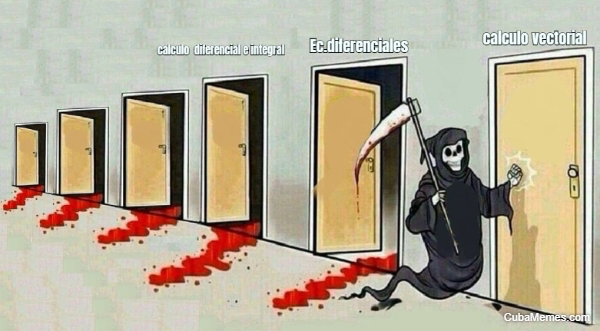
\includegraphics[width=.5\textwidth]{imagenes/imagenescv/xisteCalcVect.png}
\end{figure}
\end{multicols}

\textcolor{gris}{ Cuatro operaciones son importantes en el cálculo vectorial: }

\textcolor{gris}{ •	Gradiente: mide la tasa y la dirección del cambio en un campo escalar; el gradiente de un campo escalar es un campo vectorial.}

\textcolor{gris}{ •	Rotor o rotacional: mide la tendencia de un campo vectorial a rotar alrededor de un punto; el rotor de un campo vectorial es otro campo vectorial.}

\textcolor{gris}{ •	Divergencia: mide la tendencia de un campo vectorial a originarse o converger hacia ciertos puntos; la divergencia de un campo vectorial es un campo escalar.}

\textcolor{gris}{ •	Laplaciano: relaciona el "promedio" de una propiedad en un punto del espacio con otra magnitud, es un operador diferencial de segundo orden.}

\textcolor{gris}{ La mayoría de los resultados analíticos se entienden más fácilmente usando la maquinaria de la geometría diferencial, de la cual el cálculo vectorial forma un subconjunto.}

\rightline{\textcolor{gris}{Fuente: Wikipedia}}



\section{Resumen de la geometría vectorial aprendida en bachillerato}


\subsection{Vectores en el espacio ($\mathbb R^3$)}


%%%%%%%%%%%%%%%%%%%%%%%%%%%%%%%%%%%%%%%%%%%
$\vec v= \overrightarrow { AB }  $: segmento orientado. Origen A y extremo B
	\begin{multicols}{2}		
	\begin{itemize}
	\item \textit{módulo}: $|\vec v|=d(A,B)$
	\item \textit{dirección}: la de la recta $r$ y la de todas las paralelas a $r$
	\item \textit{sentido}: desde $A$ hacia $B$
	\end{itemize}
	\begin{figure}[H]
		\centering
		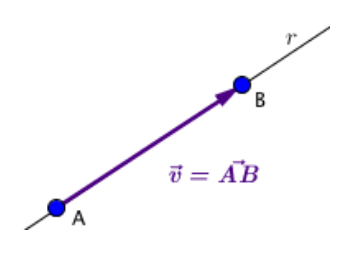
\includegraphics[width=0.4\textwidth]{imagenes/imagenescv/T10IM01.png}
	\end{figure}
	\end{multicols}

Vectores LIBRES, se pueden trasladar paralelamente a sí mismos por todo el espacio.
				
Dos vectores son IGUALES si tienen el mismo módulo, la misma dirección y el mismo sentido.

\subsection{Producto de un vector por un número real (escalar)}

$k \in \mathbb{R}$: $\ \ k\cdot \vec v$
\begin{multicols}{2}				
\begin{itemize}
	\item \textit{módulo}: $|k|\cdot |\vec v|$
	\vspace{-2mm}\item \textit{dirección}: la misma que $\vec v$
	\vspace{-2mm}\item \textit{sentido}: si $k>0$ mismo que $\vec v$; si $k<0$ contrario a $\vec v$
\end{itemize} 
\begin{figure}[H]
		\centering
		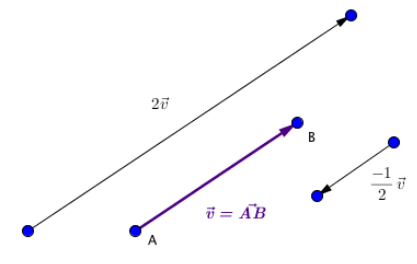
\includegraphics[width=0.3\textwidth]{imagenes/imagenescv/T10IM02.png}
\end{figure}
\end{multicols}


Dado un vector $\vec v$, un vector UNITARIO en la misma dirección que $\vec v$ se puede obtener como: $\dfrac 1 {|\vec v|}\cdot \vec v$

\vspace{4mm}

\underline{Propiedades:} 

\begin{itemize}
\begin{multicols}{2}
	\item $a\cdot (b\cdot \vec v)=(a\cdot b)\cdot \vec v$ 
	\item  $a\cdot (b\cdot \vec v)=(a\cdot b)\cdot \vec v$ 
	\item $(a+b)\cdot \vec v=a\cdot \vec v+ b\cdot \vec v  $
	\item $1\cdot \vec v=\vec v$
\end{multicols}
\end{itemize}

\subsection{Suma de vectores}

	$\vec u \pm \vec v$  (gráficamente: en matemáticas se usa la técnica de vectores concurrentes, en física es más usual el método del paralelogramo).
	\begin{multicols}{2}
	
	\begin{itemize}
		\item $(\vec u + \vec v)+ \vec w=\vec u+(\vec v + \vec w)$
		\vspace{-2mm}\item $\vec u + \vec v= \vec v+ \vec u$
		\vspace{-2mm}\item $\vec u+ \vec 0=\vec u$
		\vspace{-2mm}\item $\vec u+ (\overrightarrow {-u})=\vec 0$
	\end{itemize}
	\begin{figure}[H]
		\centering
		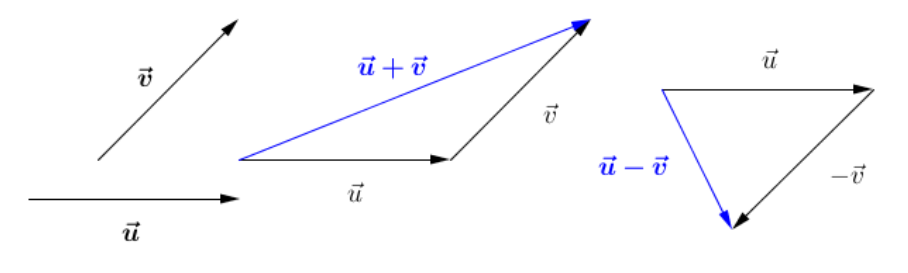
\includegraphics[width=0.5\textwidth]{imagenes/imagenescv/T10IM03.png}
	\end{figure}
	\end{multicols}
	Restar vectores = sumar el opuesto : $\vec u - \vec v = \vec u +(-\vec v)$

\begin{multicols}{2}
	\scriptsize{Puesto que los vectores con que tratamos son libres, el `método del paralelogramo' usado en física consiste en colocar los vectores unidos por sus orígenes y, mediante paralelas a éstos, construir un paralelogramo. El vector que va desde la unión de los vectores al punto opuesto de la diagonal es el vector suma}  \normalsize{:}

	\begin{figure}[H]
	\centering
	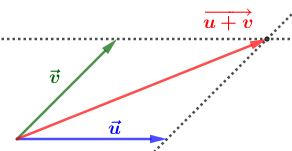
\includegraphics[width=0.3\textwidth]{imagenes/imagenescv/T10IM14.png}
	\end{figure}
\end{multicols}

\begin{multicols}{2}
	\begin{figure}[H]
	\centering
	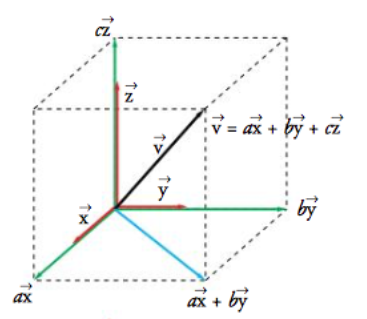
\includegraphics[width=0.30\textwidth]{imagenes/imagenescv/T10IM04.png}
	\end{figure}
	
	La suma de tres vectores de distinta dirección y no coplanarios en el espacio: 
	
	\centerline{$\vec u+\vec v+\vec w$} 
	
	es la diagonal del paralelepípedo.
\end{multicols}

\subsection{Combinación lineal de vectores}

	Dados varios vectores $\vec u_1$, $\vec u_2$, $\vec u_3$, ..., $\vec u_n$ y otros tantos números reales $\alpha_1$, $\alpha_2$, $\alpha_3$, ..., $\alpha_n$, a la expresión $\alpha_1 \vec u_1+\alpha_2 \vec u_2+\alpha_3 \vec u_3+...+\alpha_n \vec u_n$ se le llama `Combinación Lineal' de los n-vectores iniciales.
		
	%\vspace{3mm}
		
	Varios vectores se dice que son `Linealmente Dependientes'  si alguno de ellos se puede poner como combinación lineal de los demás. Si no es así, se dice que son `Linealmente Independientes'.
	

\subsection{Base}

\begin{multicols}{2}
	3 vectores cualesquiera del espacio, no coplanarios, y de direcciones distintas, $\vec x,\ \vec y, \ \vec z$ son linealmente independientes, además, cualquier otro vector del espacio se puede escribir como combinación lineal de estos tres vectores de forma única. Se dice que estos tres vectores forman una BASE $B=\{\vec x,\ \vec y, \ \vec z\}$
	\begin{figure}[H]
	\centering
	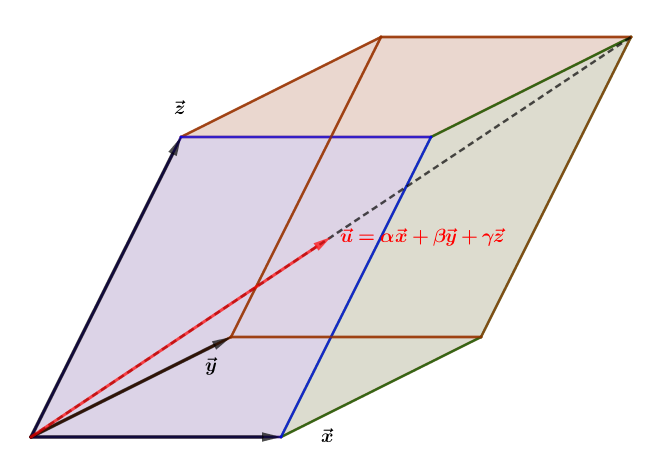
\includegraphics[width=0.40\textwidth]{imagenes/imagenescv/T10IM06.png}
	\end{figure}
\end{multicols}

\vspace{3mm}

\begin{multicols}{2}
	\begin{figure}[H]
	\centering
	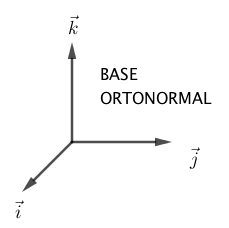
\includegraphics[width=0.25\textwidth]{imagenes/imagenescv/T10IM05.png}
	\end{figure}
	Si los vectores de la base son mutuamente perpendiculares (ortonormales) y tienen módulo 1 (unitarios), la base $B=\{\vec i, \vec j, \vec k \}$ se llama `Base OrtoNormal (BON)' 
	\footnotesize{(Orto por ortogonal, es decir, perpendiculares entre sí, y Normal porque los vectores básicos tiene norma o módulo $1$, están normalizados)}\normalsize{.}
\end{multicols}

\subsection{Operaciones con vectores dados por sus componentes}

Como cualquier vector $\vec v$  se puede expresar de forma única en cada base $B=\{\vec x,\ \vec y, \ \vec z\} \quad \to \quad \vec v= \alpha \vec x+ \beta \vec y+ \gamma \vec z$. A los parámetros de esta combinación lineal, $\alpha, \ \beta, \ \gamma$ se les llama \underline{componentes} de $\vec v$ en la base $B$, $\ \vec v=(\alpha, \ \beta, \ \gamma)$
		
Las componentes de $\vec i, \ \vec j, \ \vec k$ en la base ortonormal $B=\{ \vec i, \vec j, \vec k \} $ son $\vec i=(1,0,0); \ \vec j=(0,1,0); \ \vec k=(0,0,1)$
		
 En el espacio, los \underline{puntos} se representan por \underline{coordenadas}, $A(x_0, y_0, z_0)$ y los \underline{vectores} por \underline{componentes} $\vec u=(u_x, u_y, u_z)$


		
\vspace{3mm} $ \alpha , \ \beta \ \in \mathbb{R}; \ \vec u=(u_x,u_y,u_z); \ \vec v = (v_x ,v_y ,v_z) \to $
		
\vspace{2mm}\hspace{20mm}$\alpha \vec u+\beta \vec v=
			(\alpha  u_x+\beta  v_x,\;  \alpha  u_y+\beta  v_y,\;  \alpha  u_z+\beta  v_z) $
			
\subsection{Producto `Escalar'}

\begin{equation}
	\boxed{\ \vec u \cdot \vec v = |\vec u| \cdot |\vec v| \cdot \cos \theta \ } \ ,\ \in \mathbb{R} 
\end{equation}			

\vspace{3mm}

\begin{multicols}{2}
Geométricamente:

\emph{El producto escalar de dos vectores es el módulo de uno de ellos por la proyección del otro sobre él}
\begin{figure}[H]
	\centering
	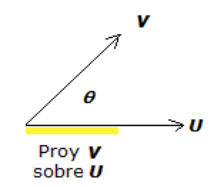
\includegraphics[width=0.2\textwidth]{imagenes/imagenescv/T10IM07.png}
\end{figure}
\end{multicols}


	Propiedad fundamental: $\forall \  \vec u,\ \vec v\ \neq 0:\ \boxed{\  \vec u \bot \vec v \ \leftrightarrow \ \vec u \cdot \vec v=0 \ }$
		
	$\vec u \cdot \vec v = \vec v \cdot \vec u$; $\ \alpha ( \vec u \cdot \vec v) =( \alpha \vec u) \cdot \vec v = \vec u \cdot ( \alpha \vec v)$; $\ \vec u \cdot (\vec v + \vec w)= \vec u \cdot \vec v + \vec u \cdot \vec w$
		
	 Módulo de un vector: $\boxed{ \ | \vec u |=+\sqrt{\vec u \cdot \vec u} \ }$
		
	 Ángulo entre dos vectores: $\boxed{ \ \cos \theta = \dfrac {\vec u \cdot \vec v}{|\vec u| \cdot |\vec v|} \ }$
	 
\vspace{4mm} \textbf{Producto escalar en B.O.N. \small{(Base orto-normal)}}

$BON=\{ \vec i, \vec j, \vec k \ / \  |\vec i|=|\vec j|=|\vec k|=1 \ \wedge \ \vec i \bot \vec j; \ \vec j \bot \vec k; \ \vec k \bot \vec i \}$. 

$\vec u=(u_1,u_2,u_3); \ \vec v=(v_1, v_2, v_3) \ \to \ $
$\boxed{  \ \vec u \cdot \vec v= u_1 v_1+u_2 v_2+u_3 v_3 \ }  \  \in \mathbb{R}$

\vspace{2mm} Módulo en una BON: $ \vec u=(u_1,u_2,u_3) \to |\vec u|=+\sqrt{u_1^2+u_2^2+u_3^2}$
		
\vspace{2mm} Ángulo \small{de dos vectores en una BON:} $\cos \theta = \dfrac {u_1 v_1+u_2 v_2+u_3 v_3}{\sqrt{u_1^2+u_2^2+u_3^2}\cdot \sqrt{v_1^2+v_2^2+v_3^2}}$

\vspace{4mm}

\begin{multicols}{2}
\textit{Normalización de un vector:} 

Dado un vector $\vec v$, conseguir otro de la misma dirección pero de módulo $1$, le llamaremos $\vec u_v$ y se obtiene como: $\vec u_v=\dfrac {1}{|\vec v|}\cdot \vec v = (\cos \alpha, \cos \beta, \cos \gamma)$, son los llamados \textit{cosenos directores} (las componentes de todo vector unitario).
\begin{figure}[H]
	\centering
	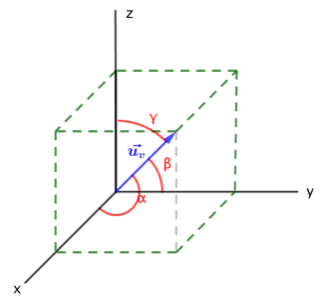
\includegraphics[width=0.30\textwidth]{imagenes/imagenescv/T10IM08.png}
\end{figure}
\end{multicols}

\subsection{Producto `Vectorial'}

El producto vectorial de dos vectores $\vec u$ y $\vec v$ es un nuevo vector $\vec u \times \vec v$	 tal que:
\begin{multicols}{2}
\begin{itemize}
\item su módulo es $|\vec u \times \vec v|=|\vec u||\vec v| \sin \theta $, siendo $\theta$ el ángulo que forman $\vec u$ y $\vec v$.
\item su dirección es perpendicular al plano que forman $\vec u$ y $\vec v$.
\item y su sentido es el del giro de un `sacacorchos' que intente llevar el vector$\vec u$ hacia el $\vec v$.
\end{itemize}
\begin{figure}[H]
	\centering
	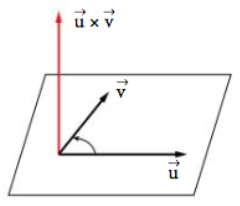
\includegraphics[width=0.30\textwidth]{imagenes/imagenescv/T10IM09.png}
\end{figure}
\end{multicols}

\textbf{Propiedades del producto vectorial.}
\begin{multicols}{2}

El \underline{módulo} del producto vectorial mide el \underline{área del paralelogramo} que forman los vectores $\vec u$ y $\vec v$.
				
\hspace{10mm}$|\vec u \times \vec v|=|\vec u||\vec v| \sin \theta$

\begin{figure}[H]
	\centering
	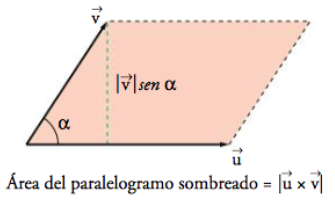
\includegraphics[width=0.30\textwidth]{imagenes/imagenescv/T10IM10.png}
\end{figure}

\end{multicols}

\begin{itemize}
	\item ¡El producto vectorial es \underline{no-conmutativo}!: $\vec u \times \vec v=-\vec v \times \vec u$
	\item $\vec u \times \vec u=\vec 0$
	\item Tomaremos la BON \underline{orientada}, $\vec i \times \vec j = \vec k$; $\vec j \times \vec k = \vec i$ y $\vec k \times \vec i = \vec j$

A esto es lo que llaman los físicos una BON `orientada', los vectores $\vec i, \vec j, \vec k$ no pueden tener orientaciones cualesquiera. 	

\item $(\alpha \vec u)\times \vec v=\alpha (\vec u \times \vec v)= \vec u \times (\alpha \vec v)$
\item ¡\underline{No} se cumple la \underline{asociativa}!: $\vec u \times (\vec v \times \vec w) \neq (\vec u \times \vec v)\times \vec w$
\item \underline{Distributivas}: $\vec u \times (\vec v + \vec w)= \vec u \times \vec v + \vec u \times \vec w$; $(\vec u + \vec v)\times \vec w=\vec u \times \vec w + \vec v \times \vec w$
\item En componentes, el desarrollo del producto vectorial es un determinante:
\begin{equation}		
\boxed{ \ \overrightarrow { u } \times \overrightarrow { v } \quad =\quad \left| \begin{matrix} \overrightarrow { i }  & \overrightarrow { j }  & \overrightarrow { k }  \\ u_1 & u_2 & u_3 \\ v_1 & v_2 & v_3 \end{matrix} \right| \ }
\end{equation}
\end{itemize}
		
\vspace{2mm}$\vec u \times \vec v$ siempre es un vector perpendicular a $\vec u$ y a $\vec v$ y su módulo representa el área del paralelogramos que defines estos dos vectores.

\vspace{5mm} ¡ Afortunadamente, el producto vectorial no es asociativo XD !

\begin{figure}[H]
	\centering
	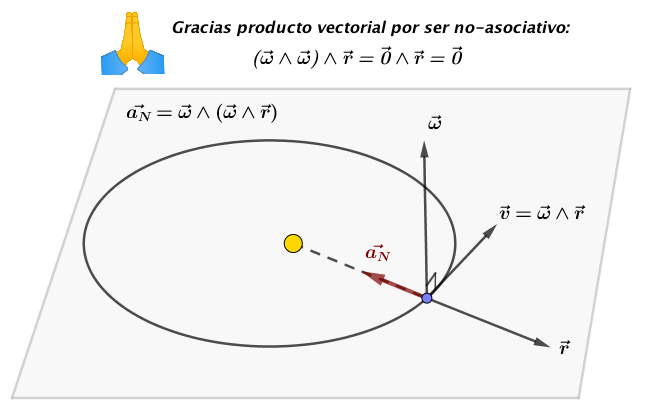
\includegraphics[width=.7\textwidth]{imagenes/imagenescv/T10IM11.png}
\end{figure}

\subsection{Producto `Mixto'}
\begin{equation}
\boxed{ \ [\vec u, \vec v, \vec w]=\vec u \cdot (\vec v \times \vec w)=|\vec u|\cdot|(\vec v \times \vec w)|\cdot \cos \theta \ }
\end{equation}

\begin{multicols}{2}
El \underline{producto mixto} $[\vec u, \vec v, \vec w]$ mide, \underline{en valor absoluto}, el \underline{volumen del paralelepípedo} formado por los tres vectores.
				
En componentes se calcula como un determinante:
				
$\boxed{ \ [\overrightarrow { u } ,\overrightarrow { v }, \overrightarrow { w }]  \quad =\quad \left| \begin{matrix} u_{ 1 } & u_{ 2 } & u_{ 3 } \\ v_{ 1 } & v_{ 2 } & v_{ 3 } \\ w_{ 1 } & w_{ 2 } & w_{ 3 } \end{matrix} \right| \ } $

\begin{figure}[H]
	\centering
	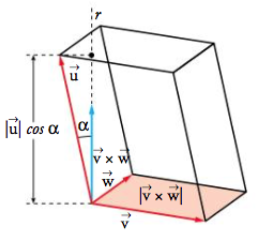
\includegraphics[width=0.3\textwidth]{imagenes/imagenescv/T10IM12.png}
\end{figure}
\end{multicols}

\begin{multicols}{2}
Por propiedades de los determinantes y del valor absoluto podemos afirmar que para el cálculo del volumen de un paralelepípedo formado por tres vectores no importa el orden en que los cojamos para calcular el producto mixto.
\begin{figure}[H]
	\centering
	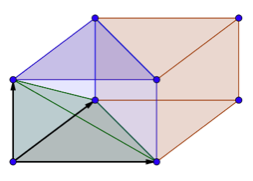
\includegraphics[width=0.25\textwidth]{imagenes/imagenescv/T10IM13.png}
\end{figure}
\end{multicols}


\subsection{Ejercicios resueltos de repaso de geometría vectorial}


\begin{miejercicio}
	
	Obtén 3 vectores perpendiculares a $\vec u=(3,2,7)$, no proporcionales entre sí.

\rule{200pt}{0.1pt}
	
	\begin{multicols}{2}
	Sabemos que  
	$  \vec u \bot \vec v \ \leftrightarrow \ \vec u \cdot \vec v=0 \ $
	y que vectores perpendiculares a uno dado hay infinitos (todo un `plano vectorial'), y que cualquier combinación de dos vectores perpendiculares a uno dado también es perpendicular a éste.
	\begin{figure}[H]
	\centering
	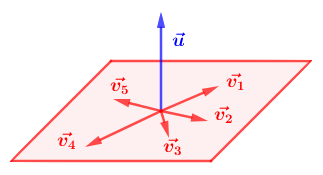
\includegraphics[width=0.30\textwidth]{imagenes/imagenescv/T10IM15.png}
	\end{figure}	
	\end{multicols}	
	Solo tenemos que encontrar vectores $\vec {v_i}$ tales que $\vec u \cdot \vec {v_i}=0$. Por ejemplo:
	
	$\vec {v_1} = (0,-7,2) \to \vec u \cdot \vec {v_1}=(3,2,7)\cdot (0,-7,2)=3 \cdot 0 + 2 \cdot (-7) + 7 \cdot 2 =-14+14=0$
	
	Compruébese que $\ \vec {v_2} = (7,0,-3);  \quad \vec {v_3} = (2,-3,0) \ $ también son perpendiculares a $\vec u$
	
	También es perpendicular a $\vec u$ cualquier combinación lineal de estos tres vectores encontrados, como p.e.:
	$\ \vec {v_4}  = \vec {v_2}+\vec {v_3}= (9,-3-3)$; incluso si lo simplificamos dividiendo por 3 (multiplicar un vector por $\frac 1 3 $  proporciona un vector de la misma dirección: $\vec {v'_4}=(3,-1,-1) \to   \ \vec u \bot \vec {v'_4} $ (\emph{compruébese}).
	
	Otro más: $\vec {v_5}=\vec {v_1} - 2 \vec {v_2}+ 3\vec {v_3}= (8,-18,8)$ (\emph{compruébese}).
\end{miejercicio}
\vspace{3mm}



\begin{miejercicio}

	Dados:  $\vec u=(1,0,-1); \vec v=(2,3,1)$. Calcular $u \cdot v; |u|; |v|; \cos \theta $

\rule{200pt}{0.1pt}
.

$u \cdot v = (1,0,-1) \cdot (2,3,1)=2+0-1=1$

$|\vec u|=+\sqrt{1^1+0^2+(-1)^2}=\sqrt{2}\; ; \quad |\vec v|=+\sqrt{2^2+3^2+1^2}=\sqrt{14}$

$\vec u \cdot \vec v = |\vec u|\cdot |\vec v| \cdot \cos \theta \to 
1=\sqrt 2 \, \sqrt{14} \; \cos \theta \to \cos \theta = \frac {\sqrt{7}}{14} \textcolor{gris}{\to \theta=79.1^o}  $

\end{miejercicio}
\vspace{3mm}	



\begin{miejercicio}
	
	Obtén un vector perpendicular a $\vec u=(3,-1,2)$ y  a $\vec v=(1,0,3)$.

\rule{200pt}{0.1pt}
	
	Lo más sencillo es buscar el vector producto vectorial de ambos: $ \vec w =\vec u \times \vec v$
	
	$\overrightarrow { w } =\left| \begin{matrix} \vec { i }  & \vec { j }  & \vec { k }  \\ 3 & -1 & 2 \\ 1 & 0 & 3 \end{matrix} \right| =[\text{ Sarrus }] =-3\vec { i } -7\vec { j } +\vec { k } =(-3,-7,1)$
\end{miejercicio}
\vspace{3mm}



\begin{miejercicio}

	Calcula el área del rectángulo de vértice  $A(2,3,7), B(1,-5,4)\  y\  C(7,0,11)$
\rule{200pt}{0.1pt}

	
Con los vértices $A, B,$ y $C$, formamos los vectores $\vec u=\overrightarrow {AB}$ y $\vec v=\overrightarrow {AC}$. Por definición del producto vectorial, el área del triángulo será igual a $ \frac 1 2 \; | \vec u \times \vec v |$

$\vec u=\overrightarrow {AB}=B-A=(-1,-8,-3)$ y $\vec v=\overrightarrow {AC}= C-A=(5, -3, 4)$.

$\overrightarrow { u \times v } =\left| \begin{matrix} \vec { i }  & \vec { j }  & \vec { k }  \\ -1 & -8 & -3 \\ 5 & -3 & 4 \end{matrix} \right| ==-41\vec { i } -11\vec { j } +43\vec { k } =(-41,-11,43)$

$|\overrightarrow { u \times v } | = \sqrt{(-41)^2+(-11)^2+(43)^2}\approx 60.42$

Área triángulo $ \approx  \frac 1 2 \; 60.41 = 30.21\; u^2$

¡Atención!: si al calcular el área de un triángulo dado por sus tres vértices el resultado es cero $\to$ ' los tres puntos están alineados'.
\end{miejercicio}

\vspace{3mm}
\begin{miejercicio}

Calcula el volumen del tetraedro cuyos vértices son: $A(-7,-2,5)$, $B(0,2,0)$, $C(-9,3,8)$  y $D(-7,5,9)$; 


\rule{200pt}{0.1pt}

Formamos los vectores:

$\vec u = \overrightarrow {AB}=B-A=(7,4,-5)$; 
$\vec v = \overrightarrow {AC}=C-A=(-2,5,3)$; 
$\vec w = \overrightarrow {AD}=D-A=(0,7,4)$

Sabemos que el valor absoluto del producto mixto de estos tres vectores es el volumen del paralelepípedo que forman, que su mitad es el volumen del prima y la sexta parte la del tetraedro, que es lo que nos piden, así que: 

Volumen tetraedro = $\frac 1 6 \left|\;  \left[ vec\quad u,\quad vec\quad v,\quad vec\quad w \; \right] \right|  =\left| \;  \left| \begin{matrix} 7 & 0 & 3 \\ -2 & 5 & 3 \\ 0 & 7 & 4 \end{matrix} \right|\;  \right| =\frac 1 6 \; |95|= \frac {95}{6} \; u^2$	
\end{miejercicio}

\vspace{3mm}
\begin{miejercicio}

	Calcula el volumen de paralelepípedo (y del prisma y del tetraedro) formado por los vectores libres $\vec u=(3,1,2), \vec v=(4,-1,0)\  y\  \vec w=(3,6,2)$

\rule{200pt}{0.1pt}
	
	$\left[ vec\quad u,\quad vec\quad v,\quad vec\quad w \right] =\left| \begin{matrix} 3 & 1 & 2 \\ 4 & -1 & 0 \\ 3 & 6 & 2 \end{matrix} \right| =40$
	
	$Vol_{paral}  = 40 \;  u^3; \quad  Vol_{prism} = \frac {40}2 =20\; u^3; \quad Vol_{tetr} = \frac {40}6 = 20/3 \; u^3$
\end{miejercicio}	


\vspace{3mm}
\begin{miejercicio}

	Calcular él ángulo que forman dos diagonales de un cubo.

\rule{200pt}{0.1pt}

\begin{multicols}{2}	
	\begin{figure}[H]
	\centering
	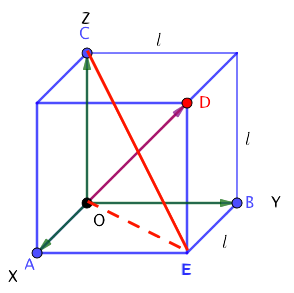
\includegraphics[width=0.25\textwidth]{imagenes/imagenescv/T10IM16.png}
	\end{figure}
De las 4 diagonales del cubo (no diagonales de las caras), elegimos las de la figura, con vectores asociados: $\overrightarrow{OD}=D-O=(l,l,l)-)0,0,0)=(1,1,1)\; l\; $ y $\overrightarrow{EC}=C-E=(0,0,l)-(l,l,0)=(1,-1,-1)\; l$

Calcule el lector el ángulo entre estos vectores con ayuda del producto escalar. \scriptsize{( $\theta \approx 109.5^0$, las diagonales, como rectas: $180-109.5=	70.5^0$)}

\end{multicols}
\end{miejercicio}



\section{Introducción al cálculo vectorial}

Para el desarrollo de esta sección me he basado en los apuntes anónimos encontrados en `http://www.cartagena99.com/recursos/examenes-ejercicios-apuntes.php' : ``Apuntes de: campos escalares y vectoriales''. También he usado los apuntes de Beléndez, Bernabeu y Partor, `Magnitudes, vectores y campos' de la UPV y encontrado en la web. Mi gratitud a todos los que comparten material en la red.

\subsection{Vector función de un escalar}

\begin{multicols}{2}
Un vector $\vec r$ es función de un escalar (número real) $t$ si lo es alguna de sus componentes:

$\boxed{ \; \vec r(t)=r_x(t) \vec i + r_y(t) \vec j + r_z(t) \vec k \; } \quad$
Tenemos una función de $\mathbb R \to \mathbb R^3\; : \; t \leadsto \vec {r(t)}$. 

Si tomamos todos los vectores con origen en $O$, sus extremos, para los distintos valores de $t$, dibujan una curva llamada `indicatriz' de ecuaciones paramétricas: $r_x=r_x(t); \; r_y=r_y(t); \; r_z=r_z(t)$. Si $t$ es el tiempo y $\vec r$ el vector de posición de una partícula, la `indicatriz' $ \vec r (t)$ será la `trayectoria'.

	\begin{figure}[H]
	\centering
	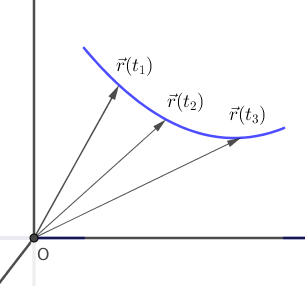
\includegraphics[width=0.25\textwidth]{imagenes/imagenescv/T10IM17.png}
	\end{figure}
\end{multicols}

\subsection{Derivada e integral de un vector}

\begin{multicols}{2}
	\begin{figure}[H]
	\centering
	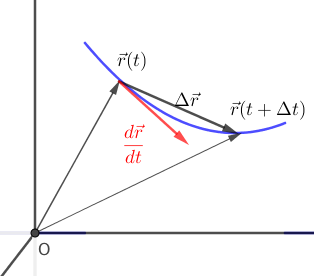
\includegraphics[width=0.3\textwidth]{imagenes/imagenescv/T10IM18.png}
	\end{figure}
Al pasar de $t$ a $t+ \Delta t \to \vec r (t)$ para a $\vec r (t+\Delta t)$ Si se incrementa la variable $t$ se incrementará el vector $\vec r$:

$\vec r (t) + \Delta \vec r = \vec r (t+\Delta t) = r_x (t+\Delta t) \vec i + r_y (t+\Delta t) \vec j + r_z (t+\Delta t) \vec k$

Despejando: $\Delta r =\vec r (t+\Delta t) - \vec r (t) = \Delta r_x \vec i +\Delta r_y \vec j +\Delta r_z \vec k \; $;  donde $\Delta r_x =  r_x (t+\Delta t) -  r_x (t) $ y análogamente para $\Delta r_y$ y $\Delta r_z$.
\end{multicols}

$\dfrac {\dd \vec r}{\dd t }= \underset{\Delta t \to 0}{lim}\; {\dfrac {\Delta r_x}{\Delta t}\;  \vec i} + \underset{\Delta t \to 0}{lim}\; {\dfrac {\Delta r_y}{\Delta t}\;  \vec j} + \underset{\Delta t \to 0}{lim}\; {\dfrac {\Delta r_z}{\Delta t}\;  \vec k}$

Es decir, la derivada de un vector respecto de un escalar es un vector cuyas componentes son las derivadas respecto del escalar de las respectivas componentes del vector a derivar.

\hspace{30mm}$\boxed{ \ \subrayado{ \  \dfrac {\dd \vec r}{\dd t }= \overrightarrow {r'} = \dfrac {\dd r_x}{\dd t}\; \vec i + \dfrac {\dd r_y}{\dd t}\; \vec j + \dfrac {\dd r_z}{\dd t}\; \vec k\  } \ }$

Por la interpretación geométrica de la derivada (\ref{IG-derivada}),el vector derivada es tangente a la curva indicatriz (trayectoria) (la dirección secante $\Delta \vec r$, con $\Delta t \to 0$ tiende a la dirección de la tangente $  \overrightarrow { r'} =\dfrac {\dd \vec r}{\dd t }\;$).

\vspace{4mm} \textbf {Reglas de derivación.} 

\begin{enumerate}[a) ]
\item Derivada de la suma de vectores: 
$\quad \dfrac {\dd {(\vec r + \vec s)}}{\dd t }$
$=\dfrac {\dd \vec r}{\dd t }+\dfrac {\dd \vec s}{\dd t }$

\item Derivada del producto por un escalar: $\quad \dfrac {\dd {(k\cdot \vec r)}}{\dd t }= k\cdot \dfrac {\dd \vec r}{\dd t }$
\item Derivada del producto escalar de dos vectores: $\quad \dfrac {\dd (\vec r \cdot \vec s)}{\dd t } = \dfrac {\dd \vec r}{\dd t }\cdot \vec s + \vec r \cdot \dfrac {\dd \vec s}{\dd t }$
\item Derivada del producto vectorial: $\dfrac {\dd (\vec r \times \vec s)}{\dd t }= \dfrac {\dd \vec r}{\dd t }\times \vec s + \vec r \times \dfrac {\dd \vec s}{\dd t }$	
\end{enumerate}

\underline{Propiedad} si $\vec r$ tiene módulo constante $\to$ es perpendicular a su vector derivada.

\vspace{-5mm} \rule{200pt}{0.1pt}

Si $\vec r (t)$ tiene módulo cte. $\vec r (t) \cdot \vec r (t)= r^2 =cte.$. Derivado este producto escalar:

$\quad \dfrac {\dd (\vec r \cdot \vec r)}{\dd t }=2\vec r \cdot \dfrac {\dd \vec r}{\dd t}=0$, ya que $\dfrac {\dd \; cte}{\dd t}=0 \Rightarrow \; \boxed{\; \subrayado{\; |\vec r|=cte \leftrightarrow \displaystyle \vec r \; \bot \;  \dfrac {\dd \vec r}{\dd t }\;} \;} $


\vspace{4mm} \textbf{Integral de un vector}. Se define como la operación inversa a la derivada de un vector: la integral de un vector $\vec r(t)=r_x(t) \vec i + r_y(t) \vec j + r_z(t) \vec k$ es otro vector cuyas componentes son las integrales de las componentes del primero.

\hspace{20mm} $\boxed{ \ \subrayado{ \  \displaystyle \int \vec r (t)\; \dd t = \vec i \; \int r_x (t)\; dd t + \vec j \; \int r_y (t)\; dd t+ \vec k \; \int r_z (t)\; dd t \ } \ }$

\subsection{Campos escalares}

Una función escalar $\phi$ que toma valores en los puntos $x,y,z)$ del espacio se dice que es una función escalar de punto o, más simplemente, un `campo escalar' si:

A cada punto $P(x,y,z)$ del espacio, la función $\phi$ le asocia un número $\phi (x,y,z)\in \mathbb R$, es una aplicación de $\mathbb R^3$ en $\mathbb R$.

Ejemplos físicos de campos escalares son la temperatura (T), la presión (P), el potencial eléctrico (V), etc. 

El conjunto de todos los puntos del plano donde el campo $\phi$ toma un determinado valor $\phi_0$ forman una `superficie equiescalar', de ecuación: $\phi=\phi_0$.

\begin{multicols}{2}
Las superficies equiescalares pueden representar puntos que están a la misma temperatura (isotermas), a la misma presión (isóbaras), al mismo potencial eléctrico (superficies equipotenciales), etc.

\footnotesize{Si el campo esta definido en un plano las equiescalares serán líneas en vez de superficies. Como ejemplo, piénsese en las curvas de nivel de un mapa topográfico, $H(x,y)$ es la altura del punto $P(x,y)$ del mapa-2D}.

	\begin{figure}[H]
	\centering
	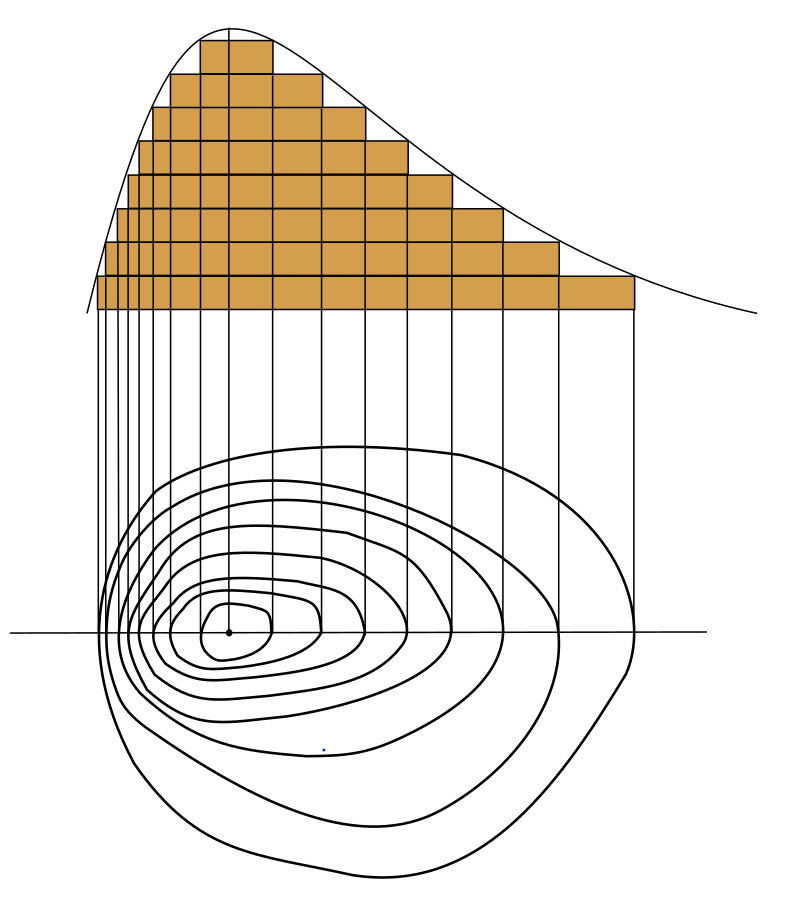
\includegraphics[width=0.25\textwidth]{imagenes/imagenescv/T10IM19.png}
	\end{figure}
\end{multicols}
\normalsize
En las funciones de una sola variable $y=f(x)$, la derivada (Leibniz) se define como el límite al que tiende el cociente $\Delta y / \Delta x$ cuando $\Delta x \to 0$, pero  un campo escalar $\phi (x,y,z)$ tendrá distintas derivadas ya que puede incrementarse una variable u otra, así, se define el crecimiento a lo largo del eje $OX$ como: $\Delta \phi_x =\phi (x+\Delta x, y, z)- \phi(x,y,z)$. Y su derivada, respecto de esta variable x, que se denota por $\dfrac{\partial \phi}{\partial x} = \underset {\Delta x \to 0}{lim}\;{\dfrac {\Delta \phi_x}{\Delta x}}= \eval {\dfrac {\dd \phi}{\dd x}}_{y,z=ctes.}\; \; $. Es decir, se trata de la derivada que resulta de suponer que $y$ y $z$ permanecen constantes y solo varía $x$. Análogamente se definen: $\dfrac{\partial \phi}{\partial y}=\eval {\dfrac {\dd \phi}{\dd y}}_{x,z=ctes.}\; $ y $\; \; \dfrac{\partial \phi}{\partial z}=\eval {\dfrac {\dd \phi}{\dd z}}_{x,y=ctes.}\; $. Esto es lo que se llama \underline{`derivadas parciales'}.

\vspace{3mm}
Las reglas de la derivación parcial son las mismas que para las funciones de una variable, solo hay que considerar que la variable sobre la que se deriva es realmente una variable y considerar al resto de vbles. como ctes.

\vspace{3mm}
Derivadas parciales: 
$\qquad \boxed{\; \subrayado{ \ \dfrac{\partial \phi}{\partial x}=\eval {\dfrac {\dd \phi}{\dd x}}_{y,z=ctes.} \quad \dfrac{\partial \phi}{\partial y}=\eval {\dfrac {\dd \phi}{\dd y}}_{z,x=ctes.} \quad \dfrac{\partial \phi}{\partial z}=\eval {\dfrac {\dd \phi}{\dd z}}_{x,y=ctes.} \ }\;} $

\section{Campos Vectoriales}
\begin{multicols}{2}
	En matemáticas, un campo vectorial representa la distribución espacial de una magnitud vectorial. Es una expresión de cálculo vectorial que asocia un vector a cada punto en $\mathbb R^3$, de la forma $\vec E: \mathbb R^3 \to \mathbb R^3 \; : \vec E (x,y,z)= E_x \vec i + E_y \vec j + E_z \vec k$
	
	Los campos vectoriales se utilizan en física, por ejemplo, para representar la velocidad y la dirección de un fluido en el espacio, o la intensidad y la dirección de fuerzas como la gravitatoria o la fuerza electromagnética.
	
	\begin{figure}[H]
	\centering
	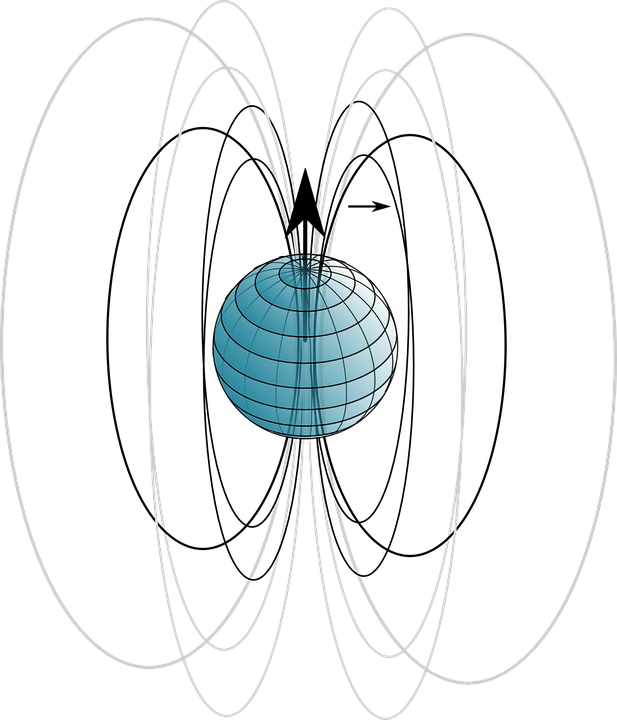
\includegraphics[width=0.35\textwidth]{imagenes/imagenescv/T10IM20.png}
	\end{figure}
\end{multicols}

\section{Gradiente de un campo escalar}

Sea $\phi (x,y,z)$ una función escalar, definida y derivable en cada uno de los puntos $(x.y.z)$ de una cierta región del espacio ($\phi$ es un campo escalar derivable), el `gradiente' de $\phi$, representado por $\overrightarrow {grad}\;  \phi\; $ o   $\; \overrightarrow{\nabla} \phi$ es un vector que se obtiene por la fórmula:

\vspace{4mm}\centerline{ $\boxed{ \subrayado{ \; \overrightarrow {grad} \; \phi =  \overrightarrow {\nabla} \phi = \dfrac {\partial \phi}{\partial x}\; \vec i +  \dfrac {\partial \phi}{\partial y}\; \vec j +  \dfrac {\partial \phi}{\partial z}\; \vec k   \;}} $}

Nótese que $\overrightarrow {grad} \; \phi $ define un `campo vectorial', es un vector que indica como varía $\phi$ en las proximidades de un punto, con el sentido del máximo crecimiento de la función.

Matemáticamente, la diferencial de una función $\phi (x.y.z)$ viene dada por:

\vspace{4mm}\centerline {$\boxed{ \subrayado{\; \dd \; \phi = \dfrac {\partial \phi}{\partial x}\; \dd x +  \dfrac {\partial \phi}{\partial y}\; \dd y + \dfrac {\partial \phi}{\partial z}\; \dd z \; }}$}

\vspace{2mm} En notación de Leibniz, $\dd \phi$ representa la variación de $\phi$ entre dos puntos muy próximos: $x,y,z)\; $ y $\; (x+\dd x. y +\dd y, z +\dd z)$. Teniendo en cuenta la definición de gradiente:

$\dd \; \phi = \dfrac {\partial \phi}{\partial x}\; \dd x +  \dfrac {\partial \phi}{\partial y}\; \dd y + \dfrac {\partial \phi}{\partial z}\; \dd z = \left( \dfrac {\partial \phi}{\partial x}\; \vec i + \dfrac {\partial \phi}{\partial y}\; \vec j + \dfrac {\partial \phi}{\partial z}\; \vec k     \right) \cdot (\dd x \; \vec i + \dd y \; \vec j + \dd z \; \vec k)$

\begin{multicols}{2}
\vspace{3mm} \begin{small} Es decir: $\quad \boxed { \subrayado{\; \dd\; \phi = \overrightarrow {grad}\; \phi \cdot \dd \; \vec r = \overrightarrow { \nabla} \; \phi \cdot \dd \; \vec r \;}} \quad$, donde $\dd \; \vec r = \dd x \; \vec i +\dd y \; \vec j + \dd z \; \vec k$, vector que une los puntos anteriormente señalados (desplazamiento infinitesimal). Esta ecuación determina la variación  $\dd \; \phi$ de la función escalar $\phi$ a lo largo de la dirección $\dd \; \vec r$. Des esta ecuación se deduce:
$\dd \; \phi = |\overrightarrow{\nabla}\; \phi |\cdot |\dd \vec r|\cdot \cos \theta$\end{small}

	\begin{figure}[H]
	\centering
	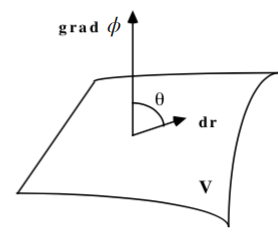
\includegraphics[width=0.3\textwidth]{imagenes/imagenescv/T10IM21.png}
	\end{figure}
\end{multicols}
\normalsize{deducimos} que, para que exista una máxima variación del campo, para un valor fijo $|\dd \vec r|$, ha de ocurrir que 
$\cos \theta=1 \to \theta = 0\; $:  

\vspace{3mm}
\begin{destacado}
\emph{`El gradiente tiene la dirección de la máxima variación del campo y va en el sentido creciente de $\phi$'}
\end{destacado}
\vspace{3mm}

Las componentes del gradiente $\overrightarrow {\nabla} \; \phi$ en la dirección de un vector unitario $\overrightarrow {u_N}$ es igual al producto escalar $\overrightarrow {\nabla} \; \phi \cdot \overrightarrow {u_N} $ y se llama \textbf{derivada direccional} de $\phi$ en la dirección de $\overrightarrow {u_N}$ :

$$\boxed{ \subrayado{\; \dfrac {\partial \phi}{\partial \overrightarrow {u_N}} = \overrightarrow {u_N} \cdot \overrightarrow {\nabla \phi}  \; }}$$

\vspace{3mm}
\begin{multicols}{2}
Para una superficie $S$ determinada por la ecuación $f(x,y,z)=0$, el vector unitario normal en el punto $(x,y,z)$ viene dado por:

\hspace{15mm} $\overrightarrow {u_N}= \dfrac {\overrightarrow {\nabla f}}{|\overrightarrow {\nabla f}|}$

	\begin{figure}[H]
	\centering
	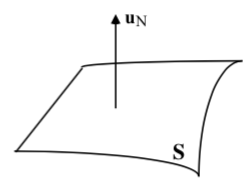
\includegraphics[width=0.25\textwidth]{imagenes/imagenescv/T10IM22.png}
	\end{figure}
\end{multicols}

La expresión: $ \overrightarrow {\nabla} \phi = \dfrac {\partial \phi}{\partial x}\; \vec i +  \dfrac {\partial \phi}{\partial y}\; \vec j +  \dfrac {\partial \phi}{\partial z}\; \vec k\;$, se puede obtener como el producto de un `operado vectorial' por un escalar , es decir:
$ \overrightarrow {\nabla} \phi = \left( \dfrac {\partial }{\partial x}\; \vec i +  \dfrac {\partial }{\partial y}\; \vec j +  \dfrac {\partial }{\partial z}\; \vec k \right) \cdot \phi\;$.
 El término dentro del paréntesis recibe el nombre de \textbf{`operado nabla'}:
\vspace{-2mm}

$$\boxed{ \subrayado{\; \overrightarrow {\nabla}=  \dfrac {\partial }{\partial x}\; \vec i +  \dfrac {\partial }{\partial y}\; \vec j +  \dfrac {\partial }{\partial z}\; \vec k \; }}$$

\vspace{3mm}En resumen, el gradiente de una función escalar es un campo vectorial que tiene las siguientes propiedades:

 \begin{enumerate}
\vspace{-3mm}
\item Sus componentes, en cada punto, son la razón de las variaciones de la función y de la coordenada a lo largo de las direcciones de los ejes en dicho punto. 
\vspace{-3mm}
\item Su módulo, en cada punto, es el máximo valor de la variación de la función con la distancia.

\vspace{-3mm}
\item Su dirección es la de máxima variación. 
\vspace{-3mm}
\item Su sentido es el de crecimiento de la función.
\vspace{-3mm}
 \end{enumerate}
 
 El gradiente es, por tanto, un campo vectorial de punto deducido de un campo escalar de punto.
 
 \subsection{Divergencia de un campo vectorial}
 
 Sea $\vec E (x,y,z)=E_x \vec i + E_y \vec j + E_z \vec k\;$, una función vectorial definida y derivable en los puntos de una determinada región del espacio, $\vec E$ es un campo vectorial derivable.
 
 La divergencia de $\vec E$, representada por $div\; \vec E\;$ ó $\overrightarrow{\nabla}\cdot \vec E$, viene dada por la expresión:
 
$$\boxed{ \subrayado{\; div\; \vec E = \overrightarrow{\nabla}\cdot \vec E = \dfrac {\partial E_x}{\partial x } + \dfrac {\partial E_y}{\partial y }+ \dfrac {\partial E_z}{\partial z } \; }}$$ 
 
 \vspace{3mm} que puede interpretarse como el `producto escalar' del operador $\overrightarrow{\nabla}$ por el campo vectorial $\vec E$, en ese orden y es, evidentemente, un escalar.
 
	La divergencia nos permite caracterizar aquellos puntos del campo vectorial en que éste, valga la expresión, `se crea o se destruye'; es decir, clasifica los manantiales o sumideros del campo. 

	Cuando $div \; \vec E = 0$ , no hay fuentes escalares del campo $\vec E$ , y se dice que el campo vectorial $\vec E$ es \textbf{\emph{solenoidal}}. 

	Si no existen `fuentes escalares' del campo éste no podrá `nacer` o `morir' en dichas fuentes, por lo cual las líneas del campo solenoidal son siempre cerradas. 

\subsection{Rotacional de un campo vectorial}

Sea $\vec E (x,y,z)=E_x \vec i + E_y \vec j + E_z \vec k\;$, un campo vectorial derivable, el rotacional de $\vec E$ , representado por $rot \; \vec E\; $ ó $\overrightarrow{\nabla} \times \vec E$ viene dado por la expresión:

\vspace{4mm} 

$\subrayado{\  rot \; \vec E = \overrightarrow{\nabla} \times \overrightarrow {E} = \left| \begin{matrix} \vec { i }  & \vec { j }  & \vec { k }  \\ \dfrac { \partial  }{ \partial x }  & \dfrac { \partial  }{ \partial y }  & \dfrac { \partial  }{ \partial z }  \\  E_{ x } & E_{ y } & E_{ z } \end{matrix} \right| \ }$

$\subrayado{\  =\left( \dfrac{\partial E_z}{\partial y} -\dfrac{\partial E_y}{\partial z} \right) \; \vec i + \left(\dfrac{\partial E_x}{\partial z} -\dfrac{\partial E_z}{\partial x} \right)\; \vec j+ \left(\dfrac{\partial E_y}{\partial x} -\dfrac{\partial E_x}{\partial y} \right)\; \vec k \ }$

\vspace{3mm}El rotacional de un vector puede entenderse como el `producto vectorial' del operador $\overrightarrow{\nabla}$ por el campo vectorial $\overrightarrow{E}$, en ese orden.

Cuando $\overrightarrow{\nabla} \times \overrightarrow {E}=\overrightarrow{0}$, se dice que el campo es \textbf{`ìrrotacional'} y nos permite decir que en campo $\overrightarrow {E}$ proviene de una función escalar $\phi$, en la forma:

$\overrightarrow{\nabla} \times \overrightarrow {E}=\overrightarrow{0} \longrightarrow \overrightarrow{E}-\overrightarrow{\nabla}\; \phi=-\overrightarrow{grad}\; \phi$

El valor del rotacional de un campo vectorial nos da las `fuentes vectoriales' del campo en cada punto. Si $\overrightarrow{\nabla} \times \overrightarrow {E}=\overrightarrow{0}$ para todos los puntos, entonces $\overrightarrow{E}$ no tiene fuentes vectoriales.

\subsection{Laplaciana de una función escalar}

Sea $\phi \; (x,y,z)$ un campo escalar definido u dos veces derivable en una determinada región del espacio. La laplaciana de $\phi$, representada por $\triangle\; \phi \;$ ó $\; \nabla^2 \; \phi$, lo determina la expresión:

$$\boxed{ \subrayado{\;\triangle\; \phi= \nabla^2 \; \phi =  \dfrac{\partial^2\; \phi}{\partial x^2}+\dfrac{\partial^2\; \phi}{\partial y^2}+\dfrac{\partial^2\; \phi}{\partial z^2} \;}}$$

\vspace{3mm} La laplaciana es una función escalar.

Análogamente al `operador nabla', podemos definir el \textbf{`operador laplaciana'} como:


$$\boxed { \subrayado{\;	 \boldsymbol{\triangle} = \nabla^2 = \dfrac {\partial^2}{\partial x^2}+ \dfrac {\partial^2}{\partial y^2}+\dfrac {\partial^2}{\partial z^2} \; }}$$

Cuando el campo escalar $\phi$ tiene derivadas segundas continuas y se cumple $\triangle \; \phi = 0$, entonces se dice que el campo escalar $\phi$ es un `campo armónico'. La ecuación  $\triangle \; \phi = 0$ se llama \textbf{ecuación de Laplace}.


\section{Ejercicios}

\begin{miejercicio}
	
Dado el campo vectorial $\overrightarrow A =x^2 \; \vec i + \sin y \; \vec j + zx \; \vec k$, encuentra: $\overrightarrow {\nabla} \cdot \overrightarrow A; \quad \overrightarrow \nabla \; (\overrightarrow {\nabla} \cdot \overrightarrow A); \quad \overrightarrow {\nabla} \times \overrightarrow A$	

\rule{200pt}{0.1pt} 

\vspace{1mm}

$\overrightarrow{\nabla}\cdot \vec A = \dfrac {\partial A_x}{\partial x } + \dfrac {\partial A_y}{\partial y }+ \dfrac {\partial A_z}{\partial z } = 3x+\cos y$	

$\overrightarrow \nabla \; (\overrightarrow {\nabla} \cdot \overrightarrow A)= \overrightarrow \nabla (3x+\cos y)= \dfrac {\partial (3x+\cos y)}{\partial x}\; \vec i + \dfrac {\partial (3x+\cos y)}{\partial y}\; \vec j +\dfrac {\partial (3x+\cos y)}{\partial z}\; \vec k = 3\; \vec i - \sin y \; \vec j$

$\overrightarrow {\nabla} \times \overrightarrow A = \left|
\begin{matrix}
\vec i & \vec j	& \vec k \\
\frac {\partial}{\partial x} & \frac {\partial}{\partial y} & \frac {\partial}{\partial z} \\
x^2 & \sin y & xz
\end{matrix}  \right|=\cdots =-z \vec i$
\end{miejercicio}

\vspace{3mm}
\begin{miejercicio}

$\overrightarrow A=2yz\; \vec i -x^2y\; \vec j +xz^2\; \vec k\; $ y $\; \phi=2x^2yz^3\; $. 

Calcula: $\overrightarrow \nabla \; \phi; \quad \overrightarrow \nabla \cdot \overrightarrow A; \quad \overrightarrow \nabla \times \overrightarrow A; \quad \overrightarrow \nabla \cdot (\overrightarrow \nabla \; \phi); \quad \overrightarrow \nabla \; (\overrightarrow \nabla \cdot \overrightarrow A) $	

\rule{200pt}{0.1pt}

\vspace{1mm}

$\overrightarrow \nabla \; \phi= \dfrac {\partial \phi}{\partial x}\; \vec i + \dfrac {\partial \phi}{\partial y}\; \vec j + \dfrac {\partial \phi}{\partial z}\; \vec k = 4xyz^3\; \vec i + 2x^2z^3\; \vec j + 6x^2yz^2\; \vec k$

$\overrightarrow \nabla \cdot \overrightarrow A=\dfrac {\partial A_x}{\partial x } + \dfrac {\partial A_y}{\partial y }+ \dfrac {\partial A_z}{\partial z }= -x^2+2xz$

$\overrightarrow \nabla \times \overrightarrow A== \left|
\begin{matrix}
\vec i & \vec j	& \vec k \\
\frac {\partial}{\partial x} & \frac {\partial}{\partial y} & \frac {\partial}{\partial z} \\
2yz & -x^2y & xz^2
\end{matrix}  \right|=\cdots =(2y-z^2) \vec j - (2xy+2z)\; \vec k$

$\overrightarrow \nabla \cdot (\overrightarrow \nabla \; \phi)= \overrightarrow \nabla \; ( 4xyz^3\; \vec i + 2x^2z^3\; \vec j + 6x^2yz^2\; \vec k)= \cdots = 4yz^3+12x^2yz$

$\overrightarrow \nabla \; (\overrightarrow \nabla \cdot \overrightarrow A)  =\overrightarrow \nabla (-x^2+2xz)=(-2x+2z)\, \vec i + 2x \; \vec k$
\end{miejercicio}

\vspace{3mm}
\begin{miejercicio}

Dado el campo escalar $\phi=(x,y,z)=2xz-3x^2+xy$, halla su derivada direccional en el pinto $(1,0,-3)$ según la dirección del vector unitario $\vec u = \widehat { u } =(-0.6,0,0.8)$ 

\rule{200pt}{0.1pt}

La derivada direccional en la dirección y sentido de un vectir unitario es la proyección del gradiente en esa dirección y sentido, es decir, su producto escalar (el de su gradiente) por dicho vector unitario.

$\dfrac {\partial \phi}{\partial \overrightarrow {u_N}} = \overrightarrow {u_N} \cdot \overrightarrow {\nabla \phi}; \quad \overrightarrow \nabla \; \phi = (-6x+y+2z) \vec i + x \vec j + 2x \vec k; \quad \eval {\overrightarrow \nabla \; \phi}|_{(1,0,-3}=(-12\vec i + \vec j + 3\vec k)$

$\eval {\dfrac { \partial \phi }{ \partial \overrightarrow {u_N} } }_{(1,0,-3)} = (-12,1,1)\cdot(-0.6,0,0.8)=8.8$
\end{miejercicio}	
\vspace{3mm}

\begin{mipropuesto}

Sea $\overrightarrow A = z \sin x \; \vec i + z \cos z \vec j + \sqrt{x^2+y^2}\; \vec k\; $, hallar:  	$\overrightarrow \nabla \; A; \quad   \overrightarrow {\nabla} \cdot \overrightarrow A; \quad \overrightarrow \nabla \; (\overrightarrow {\nabla} \cdot \overrightarrow A); \quad \overrightarrow {\nabla} \times \overrightarrow A; \quad \text { y } \quad \overrightarrow {\nabla} \times ( \overrightarrow \nabla \; A )\; $  donde $A =+\sqrt{\overrightarrow A \cdot \overrightarrow A}$, es el módulo de $\overrightarrow A$
\end{mipropuesto}

\textcolor{gris}{Sol: $A=r; \quad \overrightarrow \nabla \; A =\dfrac {x\vec i + y \vec j + z \vec k}{\sqrt{x^2+y^2+z^2}}=\vec r; \quad \overrightarrow \nabla \cdot \overrightarrow A= 0 $}

\textcolor{gris}{$\quad \overrightarrow \nabla (\overrightarrow \nabla \cdot \overrightarrow A)=\dfrac {2}{\sqrt{x^2+y^2+z^2}}=\dfrac 2 r ;\qquad \overrightarrow \nabla \times (\overrightarrow \nabla A ) =0$}


\textcolor{gris}{$ \quad \overrightarrow \nabla \times \overrightarrow A= \left( \dfrac {y}{\sqrt{x^2+y^2}-\cos z + z \sin z} \right)\; \vec i + \left (\sin z + z \cos z - \dfrac {x}{\sqrt{x^2+y^2}}  \right)\; \vec j$}

\vspace{3mm}
\begin{mipropuesto}

Dado el campo escalar $\; \phi=x^2yz+3x^2\; $ calcular su gradiente, la divergencia del gradiente y el rotacional del gradiente.

\end{mipropuesto}

\textcolor{gris}{Sol: $\overrightarrow \nabla \phi= (2xyz+6x)\vec i+x^2z\vec j+x^2y\vec k; \quad \overrightarrow \nabla \cdot(\overrightarrow \nabla \phi) = 2yz+6 ; \quad \overrightarrow \nabla \times (\overrightarrow \nabla \phi) =0$}

\section{Los conceptos de campo}

\begin{scriptsize}

\textcolor{gris}{ Reproduzco, por su interés, un artículo de }
\textcolor{gris}{https://culturacientifica.com/2016/03/29/los-conceptos-campo/, de EXPERIENTIA DOCET -ELECTROMAGNETISMO - (ARTÍCULO 8 DE 34) ,de la Cátedra de Cultura Científica de la Universidad del País Vasco.}
\textcolor{gris}{ Experientia docet (blog) es el pseudónimo de César Tomé López,  licenciado en ciencias químicas (Universidad de Granada, 1989). César Tomé López es divulgador científico y editor dE Mapping Ignorance.}
\end{scriptsize}
\vspace{4mm}

\color{ForestGreen!80}
\rule{250pt}{0.2pt}

\textbf{Los conceptos de campo}

Gilbert describió la acción de la piedra imán diciendo que tenía una “esfera de influencia” alrededor de ella. Con esto quería decir que cualquier otro objeto magnético que entrase en esta “esfera” sería atraído por la piedra imán. Además, la intensidad de la fuerza atractiva sería mayor cuanto más cercano estuviese del imán. En términos actuales diríamos que la piedra imán está rodeada por un campo magnético. Experimentalmente podemos visualizar fácilmente un campo magnético o, más precisamente, la parte del mismo que intersecta el plano de una mesa, colocando sobre ésta un imán (idealmente con una forma regular) y esparciendo limaduras de hierro alrededor.

	\begin{figure}[H]
	\centering
	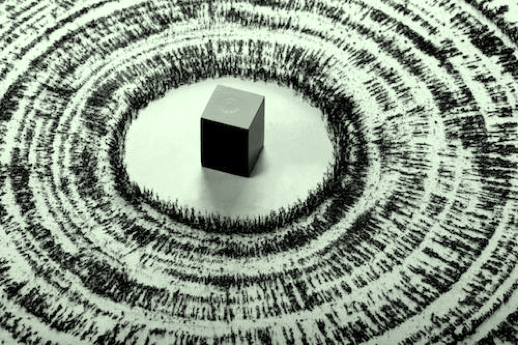
\includegraphics[width=.75\textwidth]{imagenes/imagenescv/ExperientiaDocet01.png}
	\end{figure}

La palabra “campo” se usa de maneras muy diversas y puede llevar a confusión, por lo que merece la pena que nos detengamos un momento en ella. Empezaremos por el uso común de la palabra para ir introduciendo después, de forma paulatina sus significados en física (efectivamente, sigue teniendo más de un sentido incluso en física). Este pequeño ejercicio nos permite de paso recordar que la mayoría de los términos usados en física son adaptaciones de palabras usadas en la vida ordinaria, pero a las que se dota de significados específicos. Otros ejemplos son velocidad, aceleración, fuerza, energía o trabajo. Comprender las diferencias entre el término físico y el común es fundamental para entender la física.

Uno de los usos comunes más frecuentes de la palabra campo (sobre todo en España) es “campo de juego” (en Iberoamérica quizás sea más frecuentemente “cancha”). Un campo de fútbol, por ejemplo, es un lugar donde dos equipos compiten según unas reglas que confinan la acción al área del campo. “Campo” en este caso significa región de interacción.

Otro uso habitual de la palabra campo se encuentra en el mundo de la geopolítica. En política internacional se habla de “esferas” o “campos” de influencia. Un campo de influencia política es también una región de interacción pero, a diferencia de un campo de juego, no posee una línea definida que marque sus límites. Unos países tienen más influencia que unos y menos que otros países. Por ello en el sentido político “campo” se refiere también a la cantidad de influencia, más en unos lugares y menos en otros. Además, en el caso político, el campo tiene una fuente, el país que ejerce la influencia.

Ya encontramos aquí similitudes con los conceptos de campo que se usan en física. Pero también con una diferencia importante. Para definir un campo en física tiene que ser posible asignar un valor numérico a la intensidad del campo en cada punto del campo. Esta parte del concepto de campo es más fácilmente entendible si consideramos dos situaciones de la vida cotidiana, primero en lenguaje ordinario y luego en términos físicos:

a) Voy andando por la acera, de noche, hacia una farola encendida. Veo que hay más luz conforme me acerco a ella.

b) Estoy quieto en una acera y oigo un coche que pasa de largo tocando la bocina de forma continua. Oigo que el sonido va aumentando de intensidad y luego disminuye.

	\begin{figure}[H]
	\centering
	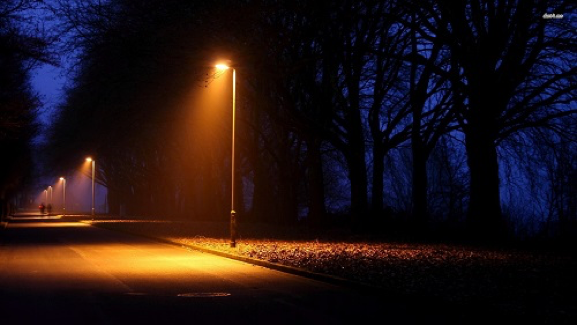
\includegraphics[width=.8\textwidth]{imagenes/imagenescv/ExperientiaDocet02.png}
	\end{figure}

Podemos describir estas dos situaciones usando campos:

a) La farola está rodeada por un campo de iluminación. Cuanto más cerca estoy de ella, más fuerte es el campo de iluminación que registra mi ojo o el medidor de intensidad de luz (fotómetro) que llevo conmigo. A cada punto del espacio alrededor de la farola puedo asignar un número que representa la intensidad del campo de iluminación en ese lugar.

b) La bocina del coche está rodeada por un campo de sonido. Yo estoy quieto en mi marco de referencia (la acera). Conforme el coche pasa a mi lado con él se mueve un patrón de valores de campo con la misma velocidad que el coche. Esto es, el campo de sonido es estable pero se mueve con la bocina. En cualquier caso yo puedo asignar un número a cada punto del campo para representar la intensidad del sonido. Al principio el sonido es apenas audible conforme la parte más débil del campo me alcanza. A partir de ahí comienza a subir la intensidad del campo y el sonido parece más fuerte. Finalmente, la intensidad disminuye al alejarse el campo de sonido y su fuente (la bocina).


Démonos cuenta de que en los campos que hemos considerado ambos están producidos por una sola fuente. En a) la fuente es una farola estacionaria y en b) es una bocina en movimiento. En ambos casos la intensidad del campo aumenta gradualmente conforme mi distancia a la fuente disminuye. Asociamos un valor numérico a cada punto del campo: estamos ante ejemplos de campos escalares sencillos. El concepto de dirección no aparece asociado al valor del campo en cada punto.

Entre los dos mapas que encuentras a continuación hay una diferencia significativa entre los campos representados en ambos. En el primero, en el que se representa la presión atmosférica y en el que las líneas (isobaras) unen puntos con igual valor de la presión, un solo número (una cantidad escalar) da el valor del campo en cada punto. Pero en el segundo, en el campo de la velocidad del viento, el valor del campo viene dado tanto por un valor numérico (llamado magnitud, representado por la escala de colores) y una dirección (representada por las flechas); la combinación de magnitud y dirección es lo que constituye un vector y por ello el campo de llama vectorial.
	
	
	\begin{multicols}{2}
	\begin{figure}[H]
	\centering
	\includegraphics[width=0.45\textwidth]{imagenes/imagenescv/ExperientiaDocet03.png}
	\caption*{Presión atmosférica}
	\end{figure}
	\begin{figure}[H]
	\centering
	\includegraphics[width=0.45\textwidth]{imagenes/imagenescv/ExperientiaDocet04.png}
	\caption*{Velocidad del viento}
	\end{figure}
	\end{multicols}


Finalmente, los físicos usan la palabra “campo” en tres sentidos adicionales a la definición de campo que hemos visto:
1) el valor del campo en un punto del espacio;
2) el conjunto de todos los valores en todos los puntos del espacio donde existe el campo;
3) la región del espacio en las que el campo toma valores distintos de cero.
Habitualmente, el contexto deja claro a cual de los conceptos de campo nos estamos refiriendo.

\vspace{-8mm}
\begin{flushright}
\rule{250pt}{0.2pt}		
\end{flushright}	
\color{black}
	





\begin{comment}

%%%%%%%%%%%%%%%%%%%%%%%%%%%%%%%%%%%. SECCIONES
\chapter{texto}
\begin{tikzpicture}
	\fill [left color=red!50, right color=teal!50] (0,0) rectangle (6.5,.2);
	\fill [left color=teal!50, right color=blue!50] (6.5,0) rectangle (11.5,.2);
	\end{tikzpicture}

\vspace{1cm}
\section{texto}
\begin{tikzpicture}
	\fill [left color=red!50, right color=teal!50] (0,0) rectangle (3.5,.1);
	\fill [left color=teal!50, right color=blue!50] (3.5,0) rectangle (7.5,.1);
	\end{tikzpicture}
\vspace{0.5cm}

\subsection{texto}
\begin{tikzpicture}
	\fill [left color=red!50, right color=teal!50] (0,0) rectangle (3.5,.01);
	\fill [left color=teal!50, right color=blue!50] (3.5,0) rectangle (7.5,.01);
	\end{tikzpicture}
\vspace{0.5cm}


%%%%%%%%%%%%%%%%%%%%%%%%%%%%%%%%%%%. \begin{ ------>. 
detsacado;  cuadro-naranja;  cuadro-gris;  miejercicio (solución extensa);  mipropuesto (solución corta y fuera del cuadro)

%%%%%%%%%%%%%%%%%%%%%%%%%%%%%%%%%%%. CURIOSIDAD
\vspace{1cm}
\color{ForestGreen!80}
\rule{250pt}{0.2pt}
Texto
\vspace{-8mm}
\begin{flushright}
\rule{250pt}{0.2pt}		
\end{flushright}	
\color{black}
\end{comment}
 %Cálculo Vectorial
\chapter{Ecuaciones paramétricas y coordenadas polares. Las cónicas en coordenadas polares}
\chaptermark{Paramétricas y Polares}

\setlength{\parindent}{0cm}

\begin{comment}
\vspace{1cm}
\section{Uno.Uno}
\begin{tikzpicture}
	\fill [left color=red!50, right color=teal!50] (0,0) rectangle (3.5,.1);
	\fill [left color=teal!50, right color=blue!50] (3.5,0) rectangle (7.5,.1);
	\end{tikzpicture}
\vspace{0.5cm}

\vspace{1cm}
\subsection{Uno.Uno.Uno}
\begin{tikzpicture}
	\fill [left color=red!50, right color=teal!50] (0,0) rectangle (3.5,.01);
	\fill [left color=teal!50, right color=blue!50] (3.5,0) rectangle (7.5,.01);
	\end{tikzpicture}
\vspace{0.5cm}
\end{comment}


	

Podemos pensar en una curva en el plano como si se tratase de la trayectoria de una partícula cuya posición varía con el tiempo, sus coordenadas $x$ e $y$ ahora se consideran funciones de una tercera variable $t$ llamada parámetro: $\ x(t), y(t)$.

\begin{figure}[H]
	\centering
	\includegraphics[width=.8\textwidth]{img-polares/polares01.png}
	\end{figure}

\vspace{-5mm}
En la figura, para una $x$ dada existe más de un valor de $y$, una recta vertical corta más de una vez a la curva por lo que no se trata de una verdadera función matemática.\footnote{Ver apartado 2.1, \textit {'Funciones reales de variable real'} del libro \textit`` {Cálculo infinitesimal \begin{scriptsize}(avanzado)\end{scriptsize} para bachillerato''}, de Ignacio Vallés Oriola, \textit{`Estrategia de la línea vertical'}. En  $\ \ $\textcolor{blau}{http://igvaori.github.io}}

Las ecuaciones paramétricas son útiles para describir curvas que no sean necesariamente funciones.

\section{Ecuaciones paramétricas}
\vspace{-5mm}
\begin{tikzpicture}
	\fill [left color=red!50, right color=teal!50] (0,0) rectangle (3.5,.1);
	\fill [left color=teal!50, right color=blue!50] (3.5,0) rectangle (7.5,.1);
	\end{tikzpicture}



\begin{cuadro-naranja}
\textbf{Curva paramétrica}: permite representar una curva en el plano mediante valores que recorren un intervalo real con una nueva variable llamada \emph{parámetro}, las coordenadas de cada punto serán funciones de este parámetro.
\vspace{-2mm}
$$C(x,y):\ \ x=x(t)\,;\ \ y=y(t)\, ; \quad \text{ con } t\in [a,b]\subset \mathbb R $$
\vspace{-2mm}
$(x(a),y(a))$ es el punto inicial de la curva, $(x(b),y(b))$ el punto final.
\vspace{2mm}
\end{cuadro-naranja}

Una misma curva admite distintas parametrizaciones.

\textsf{Cualquier función $\ y=f(x) \ $ puede parametrizarse de forma natural haciendo $\ x(t)=t\, ;\ \ y(t)=f(t) \ $ siendo el dominio del parámetro el mismo que el de la función.}

\vspace{5mm}
\begin{miejercicio}
	
Dibujar la curva $\ \ x=t^2\, ; \ \ y=t+1 \qquad -\infty<t<\infty$

\rule{300pt}{0.2pt}
	
	\begin{figure}[H]
	\centering
	\includegraphics[width=.6\textwidth]{img-polares/polares02.png}
	\end{figure}
\end{miejercicio}

\underline{Observaciones}:
\begin{itemize}
\item Al ser el intervalo del parámetro no acotado, la curva no tiene ni punto inicial ni final. 
\item Los intervalos de tiempo de la tabla son iguales pero los puntos sobre el arco de la curva no están igualmente espaciados. \hspace{3mm} \emph{Interpretación}: La partícula reduce su velocidad a medida que se acerca al eje $y$ por la rama inferior de la curva y, una vez llegado a él en el punto (0,1), se aleja	 aumentando la velocidad por la rama superior (orientación de la curva).
\item Si eliminamos el parámetro $t$ de la ecuación de la curva (\emph{esto no siempre puede hacerse}) obtenemos la ecuación rectangular o cartesiana de la misma: 
$\ \ y=t+1 \to t=y-1 \quad\Rightarrow \quad x=(y-1)^2 \, , \ $ que es la ecuación de una parábola horizontal con vértice en $(0,1)$.

\item \emph{Compruébese} que la parametrización $\ x=m^2-2m+1\, ; \ \ y=m\ \quad -\infty<m<\infty\ $ conduce a la misma curva.
\end{itemize}



\vspace{5mm}


\begin{miejercicio}

Dibujar la curva $\ \ C(x,y):\quad x=3\cos t\, ; \ \ y=3\sin t \qquad 0\le t\le 2\pi$	

\rule{300pt}{0.2pt}

\begin{figure}[H]
	\centering
	\includegraphics[width=.7\textwidth]{img-polares/polares03.png}
	\end{figure}
\end{miejercicio}

\underline{Observaciones}:
\begin{itemize}
\item Como $\ x^2+y^2=(3\cos t)^2+(3\sin t)^2=9(\cos^2 t+\sin^2 t)=9=3^2\, , \ $ se trata de la ecuación de una circunferencia de radio $3$  centrada en el origen de coordenadas.	
\item La curva empieza y acaba en $(0,1)$ y da una vuelta completa a la circunferencia en sentido \emph{levógiro} (contrario a las agujas del reloj).
\end{itemize}


\vspace{5mm}


\begin{miejercicio}

Dibujar la curva $\ \ C(x,y):\quad x=t+\dfrac 1 t\, ; \ \ y=t-\dfrac 1 t \qquad t>0$	

 \rule{300pt}{0.2pt}

\begin{figure}[H]
	\centering
	\includegraphics[width=.5\textwidth]{img-polares/polares04.png}
	\end{figure}
\end{miejercicio}

\underline{Observaciones}:
\begin{itemize}
\item Para valores pequeños de $t \ (0<t<1)$, la trayectoria está en el cuarto cuadrante y sube al primer cuadrante cuando t aumenta $(t>1)$. Al ser el dominio $]0,+\infty[$, no hay ni punto inicial ni final.
\item Eliminar el parámetro para encontrar la ecuación cartesiana de la curva es, en este caso, más difícil:

\vspace{3mm}
$\begin{cases} 
	\ x-y=\left( t+\dfrac 1 t \right) - \left( t-\dfrac 1 t \right)=\dfrac 2 t \\ 
	\  x+y=\left( t+\dfrac 1 t \right) + \left( t-\dfrac 1 t \right)=2 t 
\end{cases} \ \Rightarrow \ (x-y)(x+y)= \ \boxed{ \ \boldsymbol{x^2-y^2} \ } = \dfrac 2 t \ 2t \ \boxed { \ \boldsymbol{=4} \ }$
\vspace{3mm}

\item La hipérbola $x^2-y^2=4$ tiene en realidad otra rama, simétrica respecto del eje $y$, a la obtenida. Los puntos de nuestra curva son solo los de la hipérbola con $x=(t+1/t)>0$ al ser $t>0$, es decir, la rama derecha de la hiperbola. 
\end{itemize}

\vspace{10mm}

\begin{mipropuesto}

Dibujar la curva $\ \ C(x,y):\quad x=h+a\cos t\, ; \ \ y=k+b\sin t \qquad 0\le t\le 2\pi$	

\end{mipropuesto}


Despejando, $\quad \cos t= \dfrac{x-h}{a}\, ; \ \ \sin t= \dfrac{y-k}{b} \ \ \text { como } \ \sin^2\theta + \cos^2 \theta = 1\, , \ \forall \theta \ \therefore$

$ \dfrac{(x-h)^2}{a^2}+\dfrac{(y-k)^2}{b^2}=1 \ \ $ que es la ecuación de una elipse centrada en $(k,k)$ de semiejes $a$ y $b$.

Si $a=b=r \ \to \ $ se obtiene la ecuación de una circunferencia de radio $r$ centrada en $(h,k)$.

\begin{figure}[H]
	\centering
	\includegraphics[width=.6\textwidth]{img-polares/polares06.png}
	\end{figure}

\begin{flushright}\textcolor{teal}{\rule{250pt}{0.2pt}}	\end{flushright}



\section{Curvas famosas \small{(en paramétricas)}}

\vspace{-5mm}
\begin{tikzpicture}
	\fill [left color=red!50, right color=teal!50] (0,0) rectangle (3.5,.1);
	\fill [left color=teal!50, right color=blue!50] (3.5,0) rectangle (7.5,.1);
	\end{tikzpicture}



\subsection{Cicloide}
\vspace{-5mm}
\begin{tikzpicture}
	\fill [left color=red!50, right color=teal!50] (0,0) rectangle (3.5,.01);
	\fill [left color=teal!50, right color=blue!50] (3.5,0) rectangle (7.5,.01);
	\end{tikzpicture}

\emph{Cicloide} es la curva que determina un punto $P$ situado sobre la superficie de un círculo de radio $r$ que gira, sin deslizamiento,  a lo largo de una recta el el plano. 

\begin{multicols}{2}
Suponemos $P$ situado sobre el origen de coordenadas cuando empieza el movimiento del círculo girando hacia la derecha. Cuando haya girado $t$ radianes, el círculo habrá recorrido sobre el eje $x$ la distancia $r\cdot t$, ya que \emph{arco=ángulo$\times$radio}	(líneas moradas en la figura).
\begin{figure}[H]
	\centering
	\includegraphics[width=.5\textwidth]{img-polares/polares07.png}
	\end{figure}
\end{multicols}

Las coordenadas del punto $P$ tras el giro de $rt$ radianes son:
$\quad P:\ \begin{cases} \ x=rt+r\cos \theta \\ \ y=r+r\sin \theta \end{cases}$
 
Como, de la figura $\ \ t+\theta=\dfrac{3\pi}2 \ \to \theta=\dfrac {3\pi}2-t \quad \Rightarrow \quad  \begin{cases} \ \boldsymbol{x=r(t-\sin t)} \\ \ \boldsymbol{y=r(1-\cos t)} \end{cases}$

\begin{figure}[H]
	\centering
	\includegraphics[width=.6\textwidth]{img-polares/polares08.png}
	\caption*{Dos primeras vueltas de la cicloide y parte de la tercera.}
	\end{figure}

\color{gris}

\vspace{5mm}
\begin{multicols}{2}
\textcolor{white}{.}\vspace{-5mm}

Si voltemos la \emph{cicloide} (cicloide invertida) se obtienen dos propiedades físicas interesantes:

\begin{figure}[H]
	\centering
	\includegraphics[width=.3\textwidth]{img-polares/polares09.png}
	\end{figure}
\end{multicols}
	
\begin{itemize}
\item De todos las curvas suaves que unen dos puntos, $O$ y $A$ a distinta altura ($A$ más bajo que $O$) la cicloide es la curva por la que una partícula sujeta solo a la fuerza de la gravedad (sin rozamiento) se deslizará en el menor tiempo posible. La \emph{cicloide} es \emph{\textbf{braquistocrona}}, curva del menor tiempo posible.
\item Aunque se suelte la partícula desde un punto intermedio del trayecto $OA$, por ejemplo desde $C$, empleará el mismo tiempo en llegar a $A$ que si la soltásemos desde $O$.	La \emph{cicloide} es \emph{\textbf{tautocrona}}, curva con el mismo tiempo, $t_{OA}=t_{CA}$ .
\end{itemize}


\begin{small}	
Un péndulo simple se define como una partícula de masa $m$ suspendida de un punto $O$ por un hilo inextensible de longitud $l$ y de masa despreciable. El periodo de un péndulo simple depende de la amplitud.

\begin{multicols}{2}
Una modificación del péndulo simple que hace que su periodo sea independiente de la amplitud consiste en hacer oscilar entre dos superficies en forma de cicliode; el hilo deja tener la forma de segmento de recta para adaptarse, en parte, a esta superficie. Es el \emph{péndulo de Huygens}, es un péndulo \textbf{\emph{isocrono}} (que se produce o se hace con un ritmo constante, con intervalos o períodos de igual duración).

\begin{figure}[H]
	\centering
	\includegraphics[width=.3\textwidth]{img-polares/polares10.png}
	\caption*{\footnotesize{Péndulo de Huygens}\normalsize{.}}
	\end{figure}
	
\end{multicols}
\end{small}

\color{black}


\subsection{Lemniscata de Bernoulli}
\vspace{-5mm}
\begin{tikzpicture}
	\fill [left color=red!50, right color=teal!50] (0,0) rectangle (3.5,.01);
	\fill [left color=teal!50, right color=blue!50] (3.5,0) rectangle (7.5,.01);
	\end{tikzpicture}


\vspace{5mm}

\normalsize{La} \emph{lemniscata} fue descrita por primera vez en 1694 por Jakob Bernoulli como la modificación de una elipse. 
\begin{multicols}{2}

Una  \emph{lemniscata} es el lugar geométrico de los puntos tales que el
producto de estas distancias a dos puntos fijos llamados  \emph{focos} es
constante. 

Bernoulli la llamó  \emph{lemniscus}, que en latín significa ``cinta colgante''. Su figura es el símbolo usado en matemáticas para representar el infinito $(\infty)$.

	\begin{figure}[H]
	\centering
	\includegraphics[width=.4\textwidth]{img-polares/polares05.png}
	\end{figure}

\end{multicols}

\subsection{Cisoide, Concoide, Nefroide, Astroide, Deltoide y Cardioide}
\vspace{-5mm}
\begin{tikzpicture}
	\fill [left color=red!50, right color=teal!50] (0,0) rectangle (3.5,.01);
	\fill [left color=teal!50, right color=blue!50] (3.5,0) rectangle (7.5,.01);
	\end{tikzpicture}

\begin{figure}[H]
	\centering
	\includegraphics[width=.7\textwidth]{img-polares/polares11a.png}
	\end{figure}
\vspace{-5mm}	
\begin{figure}[H]
	\centering
	\includegraphics[width=.7\textwidth]{img-polares/polares11b.png}
	\end{figure}


\begin{table}[H]
\scriptsize
\centering
\begin{tabular}{|l|l|l|}
\hline
\multicolumn{1}{|c|}{\textbf{Cisoide}} & \multicolumn{1}{c|}{\textbf{Concoide}} & \multicolumn{1}{c|}{\textbf{Nefroide}} \\ \hline
$x=2\sin^2 t;\   y=2\sin^3 t/\cos t$ & $x=1+\cos t;\ y=\sin t + \tan t$ & $x?3\cos t-\ cos (3t);\ y=4 \sin^3 t$ \\ \hline
\multicolumn{1}{|c|}{\textbf{Astroide}} & \multicolumn{1}{c|}{\textbf{Deltoide}} & \multicolumn{1}{c|}{\textbf{Cardioide}} \\ \hline
$x=\cos^3 t;\ y=\sin^3 t$ & $x=2\cos t+\cos(2t);\ y= 2\sin t-\sin(2t)$ & $x=(\cos t+1)\cos t;\ y=(\cos t+1)\sin t$ \\ \hline
\end{tabular}
\end{table}

%\vspace{5mm} 
Otras curvas en paramétricas, dibujadas con el applet de geogebra \emph{'parametricas.ggb'} que se adjunta con estos apuntes.


\begin{figure}[H]
	\centering
	\includegraphics[width=.8\textwidth]{img-polares/polares12.png}
	\end{figure}
	
	\begin{figure}[H]
	\centering
	\includegraphics[width=.75\textwidth]{img-polares/polares13.png}
	\end{figure}

\begin{mipropuesto}

Determina las ecuaciones paramétricas de una partícula que empieza su movimiento en $(a,0)$	y recorre la elipse de ecuación $x^2/a^2\, + \, y^2/b^2=1$,
a) una vez en sentido levógiro; b) dos veces en sentido dextrógiro.

%\hspace{2.5cm} \rule{300pt}{0.2pt}

\end{mipropuesto}


$ \ \ a)\quad x=a\cos t\, , \ \ y=b\sin t \quad 0\le t\le 2\pi \qquad \qquad b)\quad x=a\cos t\, , \ \ y=-b\sin t \quad 0\le t\le 4\pi$


\begin{mipropuesto} 

\begin{multicols}{2}
Obtener la parametrización del segmento de recta que une los puntos $(0,2)$ con $(4,0)$ usando como parámetro el ángulo $\theta$ de la figura adjunta.
\begin{figure}[H]
	\centering
	\includegraphics[width=.25\textwidth]{img-polares/polares15.png}
	\end{figure}	
\end{multicols}
\end{mipropuesto}

$\ \ \begin{cases}
\ \tan \theta =\dfrac y x \to y=x\tan \theta \\
\ r:\ \begin{cases} \ (0,2) \\ \ (4,0) \end{cases} \ y=-\dfrac 1 2 x + 2
\end{cases} \ \to \ x\tan \theta =-\dfrac 1 2 x + 2 \ \Rightarrow  \quad \begin{cases} 
 \ \boldsymbol{x=\dfrac{4}{1+2\tan \theta}}	 \\  \\ \ \boldsymbol{y=\dfrac{4\tan \theta}{1+2\tan \theta}}
 \end{cases}$


\begin{figure}[H]
	\centering
	\includegraphics[width=.75\textwidth]{img-polares/polares14.png}
	\end{figure}

\vspace{-5mm}
\begin{flushright}\textcolor{teal}{\rule{250pt}{0.2pt}}	\end{flushright}\vspace{5mm}

%\vspace{5mm}
\section{Cálculo con curvas en paramétricas}

\vspace{-5mm}
\begin{tikzpicture}
	\fill [left color=red!50, right color=teal!50] (0,0) rectangle (3.5,.1);
	\fill [left color=teal!50, right color=blue!50] (3.5,0) rectangle (7.5,.1);
	\end{tikzpicture}
\vspace{0.5cm}


\large{\textbf{Recta tangente}} \normalsize{en} $(x_0,y_0):\qquad y-y_0=\eval{f'(x)}_{x_0} \cdot (x-x_0)$


En paramétricas: $\ (x(t),y(t))\ $ El punto $(x_0,y_0)$ se alcanza para algún(os) valor(es) del parámetro $t:\ \ \exists \, t_0\, / \, x(t_0)=x_0 \ \wedge \ y(t_0)=y_0$

Por otro lado, por la regla de la cadena, $\ \displaystyle \dv{y}{t}=\dv{y}{x}\dv{x}{t}$


Despejando, $ \ \ \displaystyle f'(x)=\dv{y}{x}= \dfrac{\dd y / \dd t}{\dd x / \dd t}\, , \ $ por lo que la ecuación de la recta tangente a la curva en $(x_0,t_0)$ será:

$$\subrayado{ \ \boxed{ \ \displaystyle  y-y(t_0) \ = \  \eval{\dfrac{\dd y / \dd t}{\dd x / \dd t}}_{t_0}\cdot (x-x(t_0)) \ } \ }$$


\vspace{5mm}

\begin{miejercicio}
	
Recta tangente al astroide  $\ x=\cos^3 t\, ; \ y=\sin^3 t \ $ en el punto $t=\pi/4$

\rule{300pt}{0.2pt}	

Nos piden la recta tangente a la curva cuando $\ t_0=\pi/4 \leftrightarrow x(\pi/4)=y(\pi/4)=\sqrt 2/4$ , es decir, en el punto $(\sqrt 2/4,\sqrt 2/4)$.

$ \begin{cases} 
\ x(t)=\cos^3 t \to \displaystyle \dv{x}{t}=-3\cos^2 t \sin t  
\\ \\ 
\ y(t)=\sin^3 t \to \displaystyle \dv{y}{t}=\ \ 3\sin^2 t \cos t 
\end{cases}  
\to  \ 
\displaystyle \dv{y}{x}=\dfrac{\dd y / \dd t}{\dd x / \dd t} =
\dfrac{3\sin^{\bcancel{2}} t \cancel{cos t}}{-3\\cos^{\cancel{2}} t \bcancel{\sin t}}= -\tan t$

\begin{multicols}{2}
$\quad$

Luego $\ \eval{\displaystyle \dv{y}{x}}_{t_0}= \eval{-\tan t}_{\pi/4}=-1 \ $ 

y la recta tangente buscada es:


$y-\dfrac{\sqrt{2}}{4}=-(x-\dfrac{\sqrt{2}}{4}) $

$\qquad  \qquad \to \ \ \boldsymbol{ y=-x+\dfrac{\sqrt{2}}{2} }$
\begin{figure}[H]
	\centering
	\includegraphics[width=.45\textwidth]{img-polares/polares16.png}
	\end{figure}
\end{multicols}
\vspace{1mm}
\end{miejercicio}

\vspace{5mm}


\large{\textbf{Área encerrada por una curva}}\normalsize{ $\ y=f(x)$ en} el intervalo $[a,b]$ es $\ \ A=\abs{\displaystyle \int_a^b f(x)\ \dd x}$

En paramétricas la curva es $\ (x(t),y(t))\ $ y los límites de integración serán $x=a\to t_0\,; \ x=b\to t_1$

$f(x)=y(t)\,; \quad \text{ Como } x=x(t) \ \to \ \dd x= \displaystyle \dv{x}{t} \dd t =x'(t)\dd t \ $ Así, el área será:

$$\subrayado{ \ \boxed{ \ 
\text{Área = } \abs{\displaystyle \int_{t_0}^{t_1} y(t)\, x'(t)\, \dd t} 
\ } \ }$$


\vspace{5mm}

\begin{miejercicio}

Área encerrada por el astroide $\ x=\cos^3 t\,, \ y=\sin^3 t\;\ \ t\in [0,2\pi]$

 \rule{300pt}{0.2pt}	


Por simetría, el área encerrada por el astroide es cuatro veces el área encerrada en el primer cuadrante \footnotesize{(es positiva, prescindimos del valor absoluto)}\normalsize{:}
\begin{multicols}{2}
$x=\cos^3 t \ \to \ \displaystyle \dv{x}{t}= 3\cos^2 t \sin t$

$\boldsymbol A=\displaystyle \int_0^1 y\, \dd x = 4 \int_0^{\pi/2} \sin^3 t\ 3\cos^2 t\, \sin t \ \dd t =12 \int_0^{\pi/2} \left( \dfrac{1-\cos 2t}{2} \right)^2 \left( \dfrac{1+\cos 2t}{2} \right)  \dd t = \dfrac 3 2 \int_0^{\pi/2} (1-\cos 2t -\cos^2 2t +\cos^3 2t) \dd t =$

\begin{figure}[H]
	\centering
	\includegraphics[width=.25\textwidth]{img-polares/polares17.png}
	\end{figure}
\end{multicols}

$\displaystyle =\dfrac 3 2 \left[
 \int_0^{\pi/2} (1-\cos 2t)\ \dd t -\dfrac 1 2 \int_0^{\pi/2} (1+\cos 2t)\ \dd t+ \int_0^{\pi/2} (1-\sin^2 t) \cos t \ \dd t \right]=$
 
 $\displaystyle =\dfrac 3 2 \left[
 \int_0^{\pi/2} (1-\cos 2t)\ \dd t -\dfrac 1 2 \int_0^{\pi/2} (1+\cos 2t)\ \dd t+ \int_0^{\pi/2} (\cos t-\sin^2 t\, \cos t ) \ \dd t \right]=$
 
 $\displaystyle =\dfrac 3 2 \left[
 \left(t-\dfrac 1 2 \sin 2t\right)- \dfrac 1 2 \left(t+\dfrac 1 2 \sin 2t\right)+ \left(\dfrac 1 2 \sin 2 t - \dfrac 1 6 \sin^3 2t\right)
  \right]_{0}^{\pi/2}= \ \boldsymbol {\dfrac {3\pi}{8}} \, \mathrm{u^2}$
\end{miejercicio}

Nota: 

Hemos usado que:  $\ \begin{cases}
 \ \sin^2 \alpha + \cos^2 \alpha &=1
 \\
 \ 	\cos^2 \alpha - \sin^2 \alpha &=\cos 2\alpha
 \end{cases} \ \ \to \ \ 
 \begin{cases}
 \ \text{sumando: } \ & \ \cos^2 \alpha = \dfrac{1+\cos 2\alpha}{2}
 \\
 \ \text{restando: } \ & \ \sin^2 \alpha = \dfrac{1-\cos 2\alpha}{2}
 \end{cases}$

\vspace{5mm}

\large{\textbf{Longitud de una arco de una curva}}\footnote{Ver apartado 8.3.3, \textit {'Cálculo de la longitud del arco de una curva'} del libro \textit`` {Cálculo infinitesimal \begin{scriptsize}(avanzado)\end{scriptsize} para bachillerato''}, de Ignacio Vallés Oriola. En  $\ \ $\textcolor{blau}{http://igvaori.github.io}}\normalsize{:}$\quad L=\displaystyle \int_a^b \sqrt{(1+f'(x))^2}\, \dd x$

En paramétricas la curva es $\ (x(t),y(t))\ $ y los límites de integración serán $x=a\to t_0\,; \ x=b\to t_1$

Como $\ x=x(t) \ \text{ e } \ y=y(t) \ \to \ \dd x=x'(t)\, \dd t \ \text{ y } \ \dd y=y'(t)\, \dd t$

$ L=\displaystyle \int_a^b \sqrt{(1+f'(x))^2}\, \dd x =
 \int_a^b \sqrt{ \left (1+ \displaystyle{\dv{y}{x}}{} \right)^2}\, \dd x =
 \int_a^b \dfrac{\sqrt{(\dd x)^2+(\dd y)^2}}{\dd x}\, \dd x= \int_a^b \sqrt{(\dd x)^2+(\dd y)^2} = \int_{t_0}^{t_1} \sqrt{x'(t)^2 \, (\dd t)^2+y'(t)^2 \, (\dd t)^2}  =  \int_{t_0}^{t_1} \sqrt{x'(t)^2+y'(t)^2} \, \dd t$


$$\subrayado{ \ \boxed{ \ \displaystyle L =  \int_{t_0}^{t_1} \sqrt{x'(t)^2+y'(t)^2} \ \dd t  = \int_{t_0}^{t_1} \sqrt{ \displaystyle \left( \dv{x}{t} \right)^2 + \left( \dv{y}{t} \right)^2  } \ \dd t \ } \ }  $$

%\vspace{5mm}

\begin{miejercicio}

Calcular la longitud del astroide: $\ x=\cos^3 t\,, \ y=\sin^3 t\;\ \ t\in [0,2\pi]$

\rule{300pt}{0.2pt}

Debido a la simetría que presenta el astroide, su longitud es 4 veces la del arco comprendido en el primer cuadrante.

$\displaystyle \left(\dv{x}{t}\right)^2=(-3\cos^2 t \sin t)^2=9\cos^4 t \sin^2 t;\qquad \left(\dv{y}{t}\right)^2=(3\sin^2 t \cos t)^2=9\sin^4 t \cos^2 t$

$\displaystyle \sqrt{\left(\dv{x}{t}\right)^2+\left(\dv{x}{t}\right)^2}=\sqrt{9\cos^2 t\sin^2 t \cancelto{1}{(\cos^2 t+\sin^2 t)}}=3|\cos t \sin t|=3\cos t\sin t \ \ (*)$

\textcolor{gris}\small{$(*):\ \ $ En el primer cuadrante, $0\leqslant t\leqslant \pi/2\, : \ \ \sin t\, \cos t\geqslant 0$}\normalsize{.}

Luego, $\ \displaystyle L=4\int_0^{\pi/2} 3 \cos t \sin t \, \dd t
=4\, \dfrac 3 2 \, \int_0^{\pi/2} \sin 2 t \, \dd t = -4\, \dfrac 3 2 \, \dfrac 1 2 \eval{\cos 2t}_0^{\pi/2}= 6\, \mathrm{u}$ 
\end{miejercicio}


\vspace{5mm}

\begin{mipropuesto}

Recta tangente a  $\ x=\sec t\, ; \ y=\tan t \ \ \ \text{ con } t\in I=]-\pi/2,\pi/2[\ $ en el punto $(\sqrt 2,1)$

\end{mipropuesto}
	
\begin{small}
$\begin{cases} \ x=sec t=\dfrac 1{\cos t}=\sqrt 2 \to \cos t =\dfrac{\sqrt 2}{2} \to \begin{cases} \ t=\pi/4 \in I \\ \ t=-\pi/4 \in I \end{cases} \\
\ y=\tan t = 1 \to \begin{cases}  t=\pi/4 \in I \\ \ t=3\pi/4 \notin I \end{cases} 
\end{cases} \hspace{-5mm} \mqty{\text{ ambas } \\ \text{ condiciones }} \to   t=\pi/4 $

Nos piden la recta tangente a la curva cuando $\ \boldsymbol{ t_0=\pi/4 \leftrightarrow (\sqrt 2,1) } $

$\begin{cases}
x(t)=\sec t=\dfrac 1{\cos t} \to \displaystyle \displaystyle \dv{x}{t}=-\dfrac 1{\cos^2 t} (-\sen t)=\dfrac{\sin t}{\cos ^2 t}
\\ \\
y(t)=\tan t \to \displaystyle \dv{y}{t}=\dfrac {1}{\cos^2 t}
\end{cases}
\displaystyle  \to  \ 
\dfrac{\dd y / \dd t}{\dd x / \dd t}=\dfrac{\dfrac {1}{\cos^2 t}}{\dfrac{\sin t}{\cos ^2 t}}=\dfrac 1{\sin t}=\displaystyle \dv{y}{x} $
\end{small}
\begin{multicols}{2}

Luego $\ \eval{\displaystyle \dv{y}{x}}_{t_0}= \eval{\dfrac{1}{\sin t}}_{\pi/4}=\dfrac{1}{\sqrt{2}/2}=\sqrt 2 \ $ 

y la recta tangente buscada es:


$y-1=\sqrt 2(x-\sqrt 2) $

$\qquad  \qquad \to \ \ \boldsymbol{ y=\sqrt{2} x-1 }$
\begin{figure}[H]
	\centering
	\includegraphics[width=.25\textwidth]{img-polares/polares16b.png}
	\end{figure}
\end{multicols}


\vspace{5mm}

\begin{mipropuesto}
	
 
Calcular el área bajo un arco de cicloide: $\quad x=a(t-\sin t)\, ;\ \ y=a(1-\cos t)$

\end{mipropuesto}

$A=\displaystyle \int_0^{2\pi} y\, \dd x=\int_0^{2\pi} y(t)\, \dv{x}{t}\, \dd t = \int_0^{2\pi} a(1-\cos t)\ a(1-\cos t) \ \dd t=a^2\int_0^{2\pi} (1-2\cos t+\cos^2 t)\, \dd t= a^2\int_0^{2\pi} \left(1-2\cos t+\dfrac{1+\cos 2t}{2} \right)\, \dd t= 	a^2\left[ \eval{t-2\sin t+\dfrac t 2 +\dfrac 1 4 \sin 2t }_0^{2\pi} \right.= \boldsymbol{ 3\pi \, a^2 }\ \mathrm{u}^2$
	
	\vspace{5mm}

\begin{mipropuesto}

Calcula la longitud de la curva $\ x=t^3\, ; \ \ y=3t^2/2\ $ en $\ 0\leqslant t\leqslant \sqrt 3$

\end{mipropuesto}

$L=\displaystyle \int_0^{\sqrt 3} \sqrt{(3t^2)^2+(3t)^2}\ \dd t = \int_0^{\sqrt 3} \sqrt{9t^4+9t^2}\ \dd t=\dfrac 3 2  \int_0^{\sqrt 3} 2\ t \, (t^2+1)^{1/2} \ \dd t = \dfrac 3 2 \ \eval{\dfrac{(t^2+1)^{3/2}}{3/2}}_0^{\sqrt{3}}=\eval{(t^2+1)^{3/2}}_0^{\sqrt{3}}=8-1=\ \boldsymbol 7\ \mathrm{u}$
	

\begin{flushright}\textcolor{teal}{\rule{250pt}{0.2pt}}	\end{flushright}

\section{Coordenadas polares}

\vspace{-5mm}
\begin{tikzpicture}
	\fill [left color=red!50, right color=teal!50] (0,0) rectangle (3.5,.1);
	\fill [left color=teal!50, right color=blue!50] (3.5,0) rectangle (7.5,.1);
	\end{tikzpicture}
\vspace{0.5cm}

Un \emph{Sistema de Coordenadas} en un conjunto de valores que permiten definir unívocamente la posición de cualquier punto de un espacio geométrico respecto de un punto denominado origen. 

Además del conocido \emph{Sistema de Coordenadas Cartesianas}, formado por dos ejes en el plano (tres en el espacio) mutuamente perpendiculares que se cortan en el origen y las coordenadas de un punto cualquiera vienen dadas por las proyecciones de la distancia entre el punto y el origen sobre cada uno de los ejes, también se usan los:

\begin{itemize}

\item \emph{Sistema de Coordenadas Polares} (2-dim): constituido por un eje que pasa por el origen, ahora llamado \emph{polo}. La primera coordenada es la distancia existente entre el origen y el punto, mientras que la segunda es el ángulo que forman el semieje $\mathcal {O}X+$, llamado \emph{eje polar}  y la recta que pasa por ambos puntos.



\item \emph{Coordenadas Cilíndricas} (generalización del sistema de coordenadas polares plano) y \emph{Coordenadas Esféricas}, ambos en 3-dim.
\end{itemize}


\begin{figure}[H]
	\centering
	\includegraphics[width=.8\textwidth]{img-polares/polares18.png}
	\end{figure}

\textsf{Las coordenadas polares son las más adecuadas en cualquier contexto donde el fenómeno a considerar esté directamente ligado con la dirección y longitud de un punto central, como en las figuras de revolución, en los movimientos giratorios, en las observaciones estelares, etc.  Muchos sistemas físicos, tales como los relacionados con cuerpos que se mueven alrededor de un punto central que los origina, son más simples y más intuitivos de modelar usando coordenadas polares. La motivación inicial de la introducción del sistema polar fue el estudio del movimiento circular y el movimiento orbital.}

\textsf{Todos los  sistemas sometidos a una fuerza central son buenos candidatos para el uso de coordenadas polares. Algunos ejemplos son las antenas radioeléctricas o los campos gravitatorios, que obedecen a la ley de la inversa del cuadrado.}

\vspace{5mm}

\begin{figure}[H]
	\centering
	\includegraphics[width=.65\textwidth]{img-polares/polares19.png}
	\end{figure}

\vspace{5mm}

\large{\textbf{Coordenadas Polares}}\normalsize{.}

\begin{multicols}{2}
El sistema de coordenadas polares se construye dibujando una serie de circunferencias concéntricas de radio conocido a intervalos regulares, así como rayos, también a intervalos regulares, tal como se muestra abajo en la figura. Este proceso es similar al que se sigue en un sistema de coordenadas rectangulares, donde se dibujan rectas verticales y horizontales a intervalos regulares en cada caso.

\begin{figure}[H]
	\centering
	\includegraphics[width=.4\textwidth]{img-polares/polares20.png}
	\end{figure}
\end{multicols}

\vspace{5mm}

\begin{cuadro-naranja}
Un punto $P(r,\theta)$ en polares se representa por $\boldsymbol r$, la distancia de P al polo (origen) $\mathcal O$, y por $\boldsymbol \theta$, él ángulo medido desde el eje polar hasta el segmento $\overline{\mathcal {O} P}$.

\emph{Si en alguna ocasión aparece un $r<0$ se interpreta como si esta distancia estuviese medida bajo un ángulo $\theta + \pi$.}
\end{cuadro-naranja}

\begin{figure}[H]
	\centering
	\includegraphics[width=.5\textwidth]{img-polares/polares21.png}
	\end{figure}
	
	
\begin{figure}[H]
	\centering
	\includegraphics[width=.9\textwidth]{img-polares/polares24.png}
	\end{figure}

Mientras que en cartesianas las coordenadas de un punto $P(x,y)$ son únicas, en polares, debido a la imprecisión en el número de vueltas para la medida de ángulos, hay infinitas formas de dar un mismo punto $P(r,\theta+\boldsymbol{2k\pi}),\ \forall k\in \mathbb Z$

\begin{itemize}
\item 	Los puntos en que $r=a=cte, \ \forall \theta$ son circunferencias centradas en el origen o \emph{polo} de radio $r=a$.
\item   Los puntos para $\theta=\theta_0=cte,\ \forall r$ son semirrectas que pasan por el \emph{polo} y forman un ángulo $\theta=\theta_0$ con el eje polar.
\end{itemize}

\large{\textbf{Relación entre coordenadas polares y cartesianas}}\normalsize{:} Tomando el \emph{polo} como origen de coordenadas cartesianas y el eje $\mathcal OX+$ como el eje polar, tenemos:

\vspace{5mm}
\begin{cuadro-naranja}
\begin{multicols}{2}
	\begin{figure}[H]
	\centering
	\includegraphics[width=.3\textwidth]{img-polares/polares22.png}
	\end{figure}
	%\textcolor{white}{$\quad$}
	\begin{equation*} \boxed{ \  \boldsymbol{
		\begin{cases} \ x=r\cos \theta \\ \ y=r\sin \theta \end{cases} \qquad 
		\begin{cases} \ r=\sqrt{x^2+y^2} \\ \ \tan \theta=\dfrac y x \end{cases}
		} \ }
	\end{equation*}
 \end{multicols}
\end{cuadro-naranja}

\vspace{10mm}

\begin{miejercicio}  

\hspace{1cm} a) Pasar a polares: $\ (1,1),\ (1,-1), \ (-\sqrt 3 , 1),\ (-5,0),\ (0,2)$; 

\hspace{1cm} b) Pasar a cartesianas:$\ (-2,\pi/3),\ (3,2\pi), (4,3\pi/2), (\sqrt 2, 5\pi/4)$

\rule{300pt}{0.2pt}

--- Cartesianas a polares:

$\triangleright \quad \boldsymbol{(1,1)} \quad x=1,\ y=1 \Rightarrow r=\sqrt{1^2+1^2}=\sqrt 2;\ \ \tan \theta=\dfrac{+1}{+1}\to \theta = \pi/4$

\hspace{5cm} $\boldsymbol{(1,1) \text{ cartesianas} \equiv (\sqrt 2, \pi/4) \text{ polares}}$

\begin{multicols}{2}
Las coordenadas polares no son unívocas: $\ (\sqrt 2,\pi/4)=(\sqrt 2, \pi/4+2k\pi), \ \forall k\in \mathbb Z$; además, si medimos la distancia negativa: $\ (\sqrt 2,\pi/4)=(-\sqrt 2,5\pi/4)=(-\sqrt 2,5\pi/4+2k\pi), \ \forall k\in \mathbb Z$
\begin{figure}[H]
	\centering
	\includegraphics[width=.3\textwidth]{img-polares/polares23.png}
	\end{figure}
\end{multicols}

$\triangleright \quad \boldsymbol{(1,-1)} \quad x=1,\ y=-1 \Rightarrow r=\sqrt 2;\  \ \tan \theta=\dfrac{+1}{-1} \ \textcolor{gris}{ \to \mqty(\sin \theta < 0 \\ \cos \theta >0) \to } \ \theta = 7\pi/4$

\hspace{5cm} $\boldsymbol{(1,-1) \text{ cartesianas} \equiv (\sqrt 2, 7\pi/4) \text{ polares}}$

$\triangleright \quad \boldsymbol{(-\sqrt 3,1)} \quad x=-\sqrt 3,\ y=1 \Rightarrow r= $\scriptsize{ $\sqrt{(-\sqrt 3)^2+1^2}$ } \normalsize{$ =$}$2;\ \ \tan \theta=\dfrac{1}{-\sqrt 3} \textcolor{gris}{\footnotesize{\to \mqty(\sin + \\ \cos -) \to}} \ \theta = 5\pi/6$

\hspace{5cm} $\boldsymbol{(-\sqrt 3,1) \text{ cartesianas} \equiv ( 2, 5\pi/6) \text{ polares}}$

$\triangleright \quad \boldsymbol{(-5,0)}\quad x=5,\ y= 0 \Rightarrow r=5,\ \ \theta=\pi$ \small{Solo mirando la representación}\normalsize{.}

\hspace{5cm} $\boldsymbol{(-5,0) \text{ cartesianas} \equiv (5, \pi) \text{ polares}}$

$\triangleright \quad \boldsymbol{(0,2)} \quad x=0,\ y= 2 \, , \ $ \small{como en el caso anterior}\normalsize{:} $r=2;\ \ \theta=\pi/2$

\hspace{5cm} $\boldsymbol{(0,2) \text{ cartesianas} \equiv (2, \pi/2) \text{ polares}}$

--- Polares a cartesianas:

$\triangleright \quad \boldsymbol{(-2,\pi/3)}\quad r=-2,\ \theta = \pi/3 \ \leftrightarrow \ r=2,\ \theta=\pi/3+\pi=4\pi/3 \ \to \begin{cases} x=2\cos(5\pi/3)=-1\\ y=2\sin(5\pi/3)=-\sqrt 3 \end{cases}$ 

\hspace{5cm} $\boldsymbol{(-2,\pi/3) \text{ polares} \equiv (-1,-\sqrt 3) \text{ cartesianas}}$

$\triangleright \quad \boldsymbol{(3,2\pi)}=(3,0) \quad $\small{Solo mirando la representación}\normalsize{:}$\ (3,0)$

\hspace{5cm} $\boldsymbol{(3,2\pi) \text{ polares} \equiv (3,0) \text{ cartesianas}}$


$\triangleright \quad \boldsymbol{(4,3\pi/2)}\quad$ \small{Solo mirando la representación}\normalsize{:}$\ (0,-4)$

\hspace{5cm} $\boldsymbol{(4,3\pi/2) \text{ polares} \equiv (0,-4) \text{ cartesianas}}$

$\triangleright \quad \boldsymbol{(2,5\pi/4)}\quad \begin{cases} x=2\cos(5\pi/4)= -\sqrt 2 \\ y=2\sin(5\pi/4)=-\sqrt 2 \end{cases}$	

\hspace{5cm} $\boldsymbol{(2,5\pi/4) \text{ polares} \equiv (-\sqrt 2,-\sqrt 2) \text{ cartesianas}}$

\end{miejercicio}

\vspace{5mm}
\begin{miejercicio} 
	

Pasar a polares: $\ x^2+(y-3)^2=9$

 \rule{300pt}{0.2pt}

$r=x\cos \theta,\ y=r\sin \theta \ \to (r\cos \theta)^2+(r \sin \theta - 3)^2=9 \ \to \  r^2 - 6 r \sin \theta  \quad r\neq 0  \ \to$

\hspace{5cm} $\boldsymbol{r=6\sin \theta}$
\end{miejercicio}

\vspace{5mm}
\begin{miejercicio} 
	

 Pasar a cartesianas: 

\hspace{2.6cm} $a) \ \  r\cos \theta =4 \ ; \qquad b)\ \   r^2=4r\cos \theta\ ; \qquad c)\ \   r=\dfrac 4{2\cos \theta - \sin \theta}$

 \rule{300pt}{0.2pt}

$\triangleright \ \ a)\quad  r\cos \theta = 4 \quad \Rightarrow  \boldsymbol{x=4}\ $ Recta vertical.

$\triangleright \ \ b)\quad   r^2=4r\cos \theta\ \Rightarrow x^2+y^2=4 x \to x^2-4x+\textcolor{red}{4} + y^2= \textcolor{red}{4} \to \boldsymbol{(x-2)^2+y^2=2^2} \ $ 
Circunferencia de centro $(2,0)$ y radio $2$.

$\triangleright \ \ c)\quad  r=\dfrac 4{2\cos \theta - \sin \theta} \to 2r\cos \theta -r\sin \theta = 4 \quad \Rightarrow  2x-y=4 \to \boldsymbol{y=2x-4} \ $ Recta de pendiente $2$ y ordenada en el origen $-4$.
\end{miejercicio}


\vspace{5mm}
\begin{mipropuesto} 

\begin{multicols}{2}
Pasar a polares:

$\quad a)\quad x^2+y^2=4$

$\quad b)\quad x=y$

$\quad c)\quad x^2+(y-2)^2=4$	

$\quad d)\quad x^2+xy+y^2=1$

Paras a cartesianas:

$\quad e)\quad r=4\cosec \theta$

$\quad f)\quad r^2\sin 2\theta=2$

$\quad g)\quad \cos^2 \theta = \sin^2 \theta$

$\quad h)\quad r=2\cos \theta-\sin \theta$
\end{multicols}
	
\end{mipropuesto}

$\triangleright \ \ a)\ \ x^2+y^2=4 \to (r\cos \theta)^2+(r\sin \theta)^2=4 \to \boldsymbol{r^2=4}$

$\triangleright \ \ b)\ \ x=y \to r\cos \theta=r\sin \theta \to \tan \theta=1 \to \boldsymbol{\theta =\pi/4 \ \ \wedge \ \ \theta = 5\pi/4}$

$\triangleright \ \ c)\ \ x^2+(y-2)^2=4 \to (r\cos \theta)^2+(r\sin \theta-2)^2=4 \to r^2-4r\sin \theta + 4=4 \to \boldsymbol{r=4\sin \theta}$

$\triangleright \ \ d)\ \ x^2+xy+y^2=1 \to (r\cos \theta)^2+(r\cos \theta r \sin \theta)+(r\sin \theta )^2=1 \to \boldsymbol{ r^2(1+\sin \theta \cos \theta )=1}$

$\triangleright \ \ e)\ \ r=4\cosec \theta \to r\sin \theta=4 \to \boldsymbol{y=4}$

$\triangleright \ \ f)\ \ r^2\sin 2\theta = 2 \to 2r\cos\theta \ r\sin \theta=2 \to 2xy=2 \to \boldsymbol{xy=1}$

$\triangleright \ \ g)\ \ \cos^2 \theta=\sin^2\theta \to r^2\cos^2 \theta=r^2\sin^2\theta \to |x|=|y| \to \boldsymbol{y=x \ \ \wedge \ \ y=-x}$ 

$\triangleright \ \ h)\ \ r=2\cos\theta -\sin \theta \to r^2=2r\cos\theta -r\sin \theta \to x^2+y^2=2x-y \to x^2-2x+y^2+y=0 \to x^2-2x\textcolor{red}{+1-1}+y^2+y+\textcolor{red}{+1/4-1/4}=0 \to (x-1)^2-1+(y+1/2)^2-1/4=0 \to \boldsymbol{(x-1)^2+(y+1/2)^2=5/4}$

\begin{flushright}\textcolor{teal}{\rule{250pt}{0.2pt}}	\end{flushright}


\section{Gráficas en coordenadas polares}

\vspace{-5mm}
\begin{tikzpicture}
	\fill [left color=red!50, right color=teal!50] (0,0) rectangle (3.5,.1);
	\fill [left color=teal!50, right color=blue!50] (3.5,0) rectangle (7.5,.1);
	\end{tikzpicture}
\vspace{0.5cm}

Para representar una curva polar, $r=r(\theta)$, usaremos el sistema de referencia polar: ``circunferencias concéntricas centradas en el polo y rayos que salen del polo a ángulos conocidos	''. \textcolor{gris}{(Otro modo de hacerlo es construir una tabla $\theta|r$, pasar a cartesianas $x|y$ y representar en un sistema de referencia cartesiano)}.

\vspace{5mm}

\begin{miejercicio} 
	
Representa la curva polar: $\ r=2\sin \theta$

 \rule{300pt}{0.2pt}


\begin{table}[H]
\centering
\begin{tabular}{c|ccccccccc}
$\boldsymbol{r}$ & $0$ & $\pi/6$ & $\pi/4$  & $\pi/3$ & $\pi/2$ & $2\pi/3$ & $3\pi/4$ & $5\pi/6$ & $\pi$ \\ \hline
$\boldsymbol{\theta}$ & $0$ & $1$ & $\sqrt 2$ & $\sqrt 3$ & $2$ & $\sqrt 3$ & $\sqrt 2$ & $1$ & $0$
\end{tabular}
\end{table}

\begin{multicols}{2}
Para $\pi<\theta<2\pi$ los valores se repiten dando $r<0$, por ejemplo:

$\theta=3\pi/2 \to r=2\sin (2\cdot 3\pi/2)=2\sin(3\pi)=2\sin(\pi)=2(-1)=-2$

Pero, $(-2,3\pi/2)=)(2,3\pi/2+\pi)=(2,\pi/2)$
\begin{figure}[H]
	\centering
	\includegraphics[width=.3\textwidth]{img-polares/polares25.png}
\end{figure}	
\end{multicols}
\end{miejercicio}

\underline{Observaciones}: \tiny{$\qquad \blacksquare \quad $}\normalsize{En} general, las curvas $\ r=2a \sin \theta\, ;\ \ r=2a\cos \theta \ $ son \emph{circunferencias} de radio $r=|a|$ centradas en $(a,\pi/2)$ y en $(a,0)$, respectivamente.



\vspace{5mm}

\begin{mipropuesto}

Representa $\ \ r=2+2\cos \theta$
\end{mipropuesto}
\begin{table}[H]
\centering
\begin{tabular}{c|ccccccccc}
$\boldsymbol{r}$ & $0$ & $\pi/4$ & $\pi/2$ & $3\pi/4$ & $\pi$ & $5\pi/4$ & $3\pi/2$ & $7\pi/4$ &  $2\pi$\\ \hline
$\boldsymbol{\theta}$ & $4$ & $2+\sqrt 2$ & $2$ & $2-\sqrt 2$ & $0$ & $2-\sqrt 2$ & $2$ & $12+\sqrt 2$ & $4$
\end{tabular}
\end{table}

\begin{multicols}{2}

\underline{Observaciones}: 
\tiny{$\qquad \blacksquare \quad $}\normalsize{En} general, 


\hspace{10mm}$r=a(1\pm \sin \theta)\, ; \ \ r=a(1\pm \cos \theta)\ $ 

\hspace{10mm}son \emph{cardioides}.

\textcolor{gris}{$f(-\theta)=f(\theta)$}, simetria respecto del eje polar (ver más adelante).
\begin{figure}[H]
	\centering
	\includegraphics[width=.25\textwidth]{img-polares/polares26.png}
\end{figure}
\end{multicols}

\vspace{5mm}
\begin{mipropuesto}

Representa $\ \ r=6+3\cos \theta$
\end{mipropuesto}

\begin{multicols}{2}

\underline{Observaciones}: 
\tiny{$\qquad \blacksquare \quad $}\normalsize{En} general, 


\hspace{10mm}$r=a \pm b \cos \theta \, ; \ \ r=a \pm b \sin \theta\, , \ \ |a|>|b| $ 

\hspace{10mm}son \emph{limaçon} o caracoles (sin rizo).


\begin{figure}[H]
	\centering
	\includegraphics[width=.2\textwidth]{img-polares/polares48.png}
\end{figure}
\end{multicols}


\vspace{5mm}
\begin{mipropuesto}

Representa $\ \ r=3+6\cos \theta$
\end{mipropuesto}

\begin{multicols}{2}

\underline{Observaciones}: 
\tiny{$\qquad \blacksquare \quad $}\normalsize{En} general, 



\hspace{10mm}$r=a \pm b \cos \theta \, ; \ \ r=a \pm b \sin \theta\, , \ \ |a|<|b| $ 

\hspace{10mm}son \emph{limaçon} o caracoles (con rizo).


\begin{figure}[H]
	\centering
	\includegraphics[width=.2\textwidth]{img-polares/polares49.png}
\end{figure}
\end{multicols}

\vspace{5mm}

\begin{mipropuesto}

Representa $\ \ r=\cos 2\theta$
\end{mipropuesto}

\begin{table}[H]
\centering
\begin{tabular}{c|ccccccccc}
$\boldsymbol{r}$ & $0$ & $\pi/6$ & $\pi/4$  & $\pi/3$ & $\pi/2$ & $2\pi/3$ & $3\pi/4$ & $5\pi/6$ & $\pi$ \\ \hline
$\boldsymbol{\theta}$ & $1$ & $1/2$ & $0$ & $-1/2$ & $-1$ & $-1/2$ & $0$ & $1/2$ & $1$
\end{tabular}
\end{table}

\begin{multicols}{2}
\underline{Observaciones}: 
\tiny{$\qquad \blacksquare \quad $}\normalsize{En} general, 

\hspace{10mm}$r=a \cos n \theta\, ; \ \ r=a  \sin n \theta\ $ 

\hspace{10mm} son \emph{rosas}. 

\hspace{10mm} de $n$ pétalos si $n$ es impar 

\hspace{10mm} o de $2n$ pétalos i $n$ par.	

\begin{figure}[H]
	\centering
	\includegraphics[width=.25\textwidth]{img-polares/polares27.png}
\end{figure}
\end{multicols}


\vspace{5mm}
\begin{mipropuesto}

Representa $\ \ r^2=4\cos 2\theta$
\end{mipropuesto}

\begin{multicols}{2}

\underline{Observaciones}: 
\tiny{$\qquad \blacksquare \quad $}\normalsize{En} general, 



\hspace{10mm}$r^2=a \cos 2\theta \, ; \ \ r^2=a \sin 2\theta\, , \ \ |a|<|b| $ 

\hspace{10mm}son \emph{lemniscatas}.


\begin{figure}[H]
	\centering
	\includegraphics[width=.3\textwidth]{img-polares/polares50.png}
\end{figure}
\end{multicols}

\vspace{5mm}
\begin{mipropuesto}

Representa $\ \ r=2\theta\, ; \qquad r=2e^{0.3\theta}$
\end{mipropuesto}


\underline{Observaciones}: 
\tiny{$\qquad \blacksquare \quad $}\normalsize{En} general, 

\hspace{10mm}$r^2=a \theta \ $ son \emph{espirales de Arquímedes}.
$\qquad \qquad$
\hspace{10mm}$r^2=a e^{b \theta} \ $ son \emph{espirales logarítmicas}.

\begin{multicols}{2}
\begin{figure}[H]
	\centering
	\includegraphics[width=.3\textwidth]{img-polares/polares51.png}
\end{figure}
\begin{figure}[H]
	\centering
	\includegraphics[width=.3\textwidth]{img-polares/polares52.png}
\end{figure}
\end{multicols}

\begin{flushright}\textcolor{teal}{\rule{250pt}{0.2pt}}	\end{flushright}	

%\color{ForestGreen}
\color{teal}
\rule{250pt}{0.2pt}

\begin{small}
Una espiral logarítmica, espiral equiangular o espiral de crecimiento es la curva definida por un objeto que se mueve con velocidad lineal constante y velocidad angular.

La característica fundamental de esta espiral es que la expansión y la rotación tienen un vínculo geométrico o exponencial. La distancia entre las espiras aumenta mucho más rápidamente que la rotación.

Otros nombres que recibe esta espiral es la de equiangular o geométrica; el primer nombre lo recibe ya que el mismo ángulo de giro, puestos a construirla, crece en progresión aritmética, mientras que el segundo nombre lo recibe por el radio que crece en progresión geométrica.

Este espiral es el que mas podemos observar en la naturaleza, en el reino vegetal, en las formas de las galaxias, en las conchas de algunas especies de moluscos, etc. Es también usado en el arte desde épocas prehistóricas\end{small}\normalsize{.}
	
\begin{figure}[H]
	\centering
\includegraphics[width=.95\textwidth]{img-polares/polares53.png}
\end{figure}

\vspace{-15mm}
\begin{flushright}
\rule{250pt}{0.2pt}		
\end{flushright}

\color{black}
\vspace{5mm}
\large{Otras curvas en polares}\normalsize{.}
	
	
\begin{figure}[H]
	\centering
	\includegraphics[width=1\textwidth]{img-polares/polares29.png}
\end{figure}

\vspace{5mm}	
\begin{multicols}{2}
$\quad$ 

Para curvas complicadas es conveniente usar un sw. adecuado.

Se incluye, con estos apuntes, el applet de \emph{geogebra} \textsf{`polares01.ggb'}.	

\begin{figure}[H]
	\centering
	\includegraphics[width=.25\textwidth]{img-polares/polares30.png}
\end{figure}
\end{multicols}

\vspace{5mm}
\textbf{\large{Simetrías}}\normalsize{:}
	
	En ocasiones, el estudio de la simetría de una curva simplifica el estudio de su representación.
\vspace{-5mm}	
\begin{itemize}
\item Si la ecuación de la curva no varía al cambiar $\theta$ por $-\theta$,	 entonces la curva es \emph{simétrica respecto del eje polar.}
\item Si la ecuación de la curva no varía al cambiar $r$ por $-r$,	 entonces la curva es \emph{simétrica respecto al polo.}
\item Si la ecuación de la curva no varía al cambiar $\theta$ por $\pi-\theta$,	 entonces la curva es \emph{simétrica respecto al rayo $\theta=\pi/2$ \textcolor{gris}{(eje $y$)}.}
\end{itemize}

	
\begin{figure}[H]
	\centering
	\includegraphics[width=1\textwidth]{img-polares/polares28.png}
\end{figure}


	

\section{Rectas y circunferencias en polares}

\vspace{-5mm}
\begin{tikzpicture}
	\fill [left color=red!50, right color=teal!50] (0,0) rectangle (3.5,.1);
	\fill [left color=teal!50, right color=blue!50] (3.5,0) rectangle (7.5,.1);
	\end{tikzpicture}
\vspace{0.5cm}
	


\subsection{Rectas}
\vspace{-5mm}
\begin{tikzpicture}
	\fill [left color=red!50, right color=teal!50] (0,0) rectangle (3.5,.01);
	\fill [left color=teal!50, right color=blue!50] (3.5,0) rectangle (7.5,.01);
	\end{tikzpicture}

\begin{multicols}{2}
$\triangleright \ \ $ Si la recta contiene al polo (pasa por él) tenemos, en cartesianas, una ecuación del tipo $\ y=mx \ $ con $ \ m=\tan \theta_0)$. pasando a polares, \textcolor{gris}{$(x=r\cos \theta\, , \ y=r\sin \theta)$}: $\ y=mx \to   r\sin \theta = m r \cos \theta \to \tan \theta=m=\tan \theta_0 \ \to \qquad  \boxed{ \ \subrayado{\theta=\theta_0} \ }\quad $ Recta, en forma polar, que pasa por el polo con ángulo $\theta_0$.
\begin{figure}[H]
	\centering
	\includegraphics[width=.3\textwidth]{img-polares/polares40.png}
\end{figure}
\end{multicols}


\begin{multicols}{2}
$\triangleright \ \ $ Sea $P_0(r_0,\theta_0)$ la proyección ortogonal del polo $\mathcal O$ sobre la recta $R$, con ello, la ecuación de $R$ es:

$$ \boxed{ \ \subrayado{ \ r\cos (\theta-\theta_0)=r_0 \ } \ } \quad \to \ \quad r=\dfrac{r_0}{\cos (\theta-\theta_0)}$$

Recta que no contiene al polo, está a distancia $r_0$ de éste y su perpendicular forma un ángulo $\theta_0$ con el eje polar.

\begin{figure}[H]
	\centering
	\includegraphics[width=.3\textwidth]{img-polares/polares35.png}
\end{figure}	
\end{multicols}

\underline{Observaciones}:
\vspace{-5mm}

\begin{itemize}
\item $\theta_0=0 \ \ \ \to \ \ \, r=\dfrac {r_0}{\cos \theta} \quad $ es una recta vertical.	
$\qquad \ \ \, $ \textcolor{gris}{Para $\ \theta_0=\pi \ \to \ r=-\dfrac d {\cos \theta}$}
\item $\theta_0=\pi/2 \ \to \ r=\dfrac {r_0}{\sin \theta} \quad $ es una recta horizontal. 
$\qquad$ \textcolor{gris}{Para $\ \theta_0=3\pi/2 \ \to \ r=-\dfrac d {\sin \theta}$}.
\end{itemize}

\vspace{-5mm}
\begin{figure}[H]
	\centering
	\includegraphics[width=.75\textwidth]{img-polares/polares41.png}
\end{figure}


\begin{miejercicio} 
	

Recta $\  \theta_0=\pi/3;\ \ r_0=2$ 

\rule{300pt}{0.2pt}

\begin{multicols}{2}
$\qquad \boldsymbol{ r\cos (\theta-\pi/3)=2}$ 

$\qquad r(\cos \theta \cos \pi/3 + \sin \theta \sin \pi/3)=2$ 

$\qquad \frac 1 2 r \cos \theta + \frac {\sqrt 3}2 \sin \theta = 2$

$\qquad \boldsymbol{x+\sqrt 3 y=4}$
\begin{figure}[H]
	\centering
	\includegraphics[width=.35\textwidth]{img-polares/polares42.png}
\end{figure}
\end{multicols}

\end{miejercicio}

\vspace{5mm}	
\subsection{Circunferencias}
\vspace{-5mm}
\begin{tikzpicture}
	\fill [left color=red!50, right color=teal!50] (0,0) rectangle (3.5,.01);
	\fill [left color=teal!50, right color=blue!50] (3.5,0) rectangle (7.5,.01);
	\end{tikzpicture}


$\triangleright \ \ $ Circunferencia con centro en el polo $\mathcal O$  y radio  $a$: 

En cartesianas: $ \ x^2+y^2=a^2 \ \to \ $ pasando a polares: $ \ (r \cos \theta)^2+(r \sin \theta)^2=a^2 \, , \ $

puesto que $\sin^2 \theta+\cos^2 \theta=1\, , \  $ se tiene:
$ \qquad \boxed{ \ \subrayado { \ \boldsymbol{r=a} \ } \ }$


\begin{multicols}{2}
\textcolor{white}{.}

$\triangleright \ \ $ Circunferencia de radio $\ a \ $ y centro en $\ P_0(r_0,\theta_0)\, $ 

por la ley de cosenos al $\mathcal O P_0 P\, :$

$$ \boxed{ \ \subrayado{ \ a^2 \ =\  r^2\, +\, r_0^2\, -\, 2\, r\, r_0\,  \cos (\theta-\theta_0) \ } \ }$$

\textcolor{white}{.}
\begin{figure}[H]
	\centering
	\includegraphics[width=.3\textwidth]{img-polares/polares36.png}
\end{figure}	
\end{multicols}


\underline{Observaciones}:
\vspace{-3mm}
\begin{itemize}
\item Si la circunferencia pasa por el origen: $\ r_0=a \ \to \ a^2=a^2+r^2-2ra\cos (\theta-\theta_0) \ \to $
 
$\to \ r^2=2ra\cos (\theta-\theta_0) \ \to \ \boldsymbol {r=2a \cos (\theta-\theta_0) } $
\item 	Si el centro está en $\mathcal OX+ \ \ \theta_0 = 0 \ \boldsymbol{r=2a \cos \theta}\, ; \quad $ si el centro está en $\mathcal OX- \ \ \theta_0 = 0 \ \boldsymbol{r=-2a \cos \theta}$
\item Si el centro está en $\mathcal OY+ \ \ \theta_0 = 0 \ \boldsymbol{r=2a \sin \theta}\, ; \quad $ si el centro está en $\mathcal OY- \ \ \theta_0 = 0 \ \boldsymbol{r=-2a \sin \theta}$
\end{itemize}


\begin{miejercicio} 
	

 Graficar $\  r=4\cos (\theta-\pi/3)$ 

 \rule{300pt}{0.2pt}

\begin{multicols}{2}
Por inspección de la ecuación 

\textcolor{gris}{$\ (r=2a \cos (\theta-\theta_0) \ $) }

concluimos que se trata de una circunferencia que pasa por el polo, de radio 2 y con centro en $(2,\pi/3)$.
\begin{figure}[H]
	\centering
	\includegraphics[width=.25\textwidth]{img-polares/polares43.png}
\end{figure}
\vspace{2mm}
\end{multicols}

\end{miejercicio}




\vspace{5mm}
\section{Cálculo en polares}

\vspace{-5mm}
\begin{tikzpicture}
	\fill [left color=red!50, right color=teal!50] (0,0) rectangle (3.5,.1);
	\fill [left color=teal!50, right color=blue!50] (3.5,0) rectangle (7.5,.1);
	\end{tikzpicture}
\vspace{0.5cm}


\vspace{5mm}

\large{\textbf{Distancia entre dos puntos}}\normalsize{:}

\begin{multicols}{2}

Por el teorema del coseno, 

\begin{adjustwidth}{30pt}{25pt}
\begin{destacado}
$  d\, (\, (r_1,\theta_1),(r_2,\theta_2)\, ) =  \\ \\\sqrt{r_1^2+r_2^2-2r_1r_2\cos(\theta_2-\theta_1)} $	
\end{destacado}
\end{adjustwidth}

\begin{figure}[H]
	\centering
	\includegraphics[width=.35\textwidth]{img-polares/polares31.png}
\end{figure}

\end{multicols}


\vspace{5mm}

\large{\textbf{Recta tangente}}\normalsize{:}

\vspace{5mm}

Parametrizando la curva,

$r=f(\theta) \to \begin{cases} 
 \ x=r\cos \theta = f(\theta)\cos \theta & \to \displaystyle \dv{x}{\theta}= f'(\theta)\cos \theta - f(\theta)\sin \theta	 \\ \\ 
 \ y=r\sin \theta = f(\theta)\sin \theta & \to \displaystyle \dv{y}{\theta}= f'(\theta)\sin \theta + f(\theta)\cos \theta
 \end{cases}$
 
 La pendiente de la recta tangente es:
 
 $$\boxed{ \ \subrayado{ \ 
 \displaystyle \eval{\dv{x}{y}}_{(r,\theta)}= \dfrac{f'(\theta)\sin \theta + f(\theta)\cos \theta}{f'(\theta)\cos \theta - f(\theta)\sin \theta}
 \ } \ }$$



\vspace{5mm}

\large{\textbf{Área bajo una curva}}\normalsize{:}

%\vspace{5mm}

\begin{multicols}{2}

$\quad$

$\qquad \boxed{ \ \subrayado{ \ A\ = \ \displaystyle \int_{\theta_1}^{\theta_2} \dfrac 1 2 \, r^2\, \dd \theta \ = \int_{\theta_1}^{\theta_2} \dfrac 1 2 \, f(\theta)^2\, \dd \theta  \ } \ }$

\begin{figure}[H]
	\centering
	\includegraphics[width=.25\textwidth]{img-polares/polares32.png}
\end{figure}

\end{multicols}




\vspace{5mm}

\begin{miejercicio} 

Calcular el área encerrada por el cardioide $ r=2(1+\cos\theta)\ $ en $[0,2\pi]$.

\rule{300pt}{0.2pt}

$A=\displaystyle \int_0^{2\pi} \dfrac 1 2 \, 4\, (1+\cos \theta)^2\, \dd \theta =\int_0^{2\pi} 2\, \left(1+2\cos \theta +\dfrac{1+\cos 2\theta}{2} \right)\, \dd \theta= \int_{0}^{2\pi} (3+4\cos \theta +\cos 2\theta)\, \dd \theta= \left[ 3\theta+4\sin\theta+\dfrac{\sin 2\theta}{2}\right]_{0}^{2\pi}=6\pi\ \mathrm{u}^2$
\end{miejercicio}

\underline{Observaciones}: \tiny{$\qquad \blacksquare \quad $}\normalsize{Área} encerrada por dos curvas: ver ejercicio siguiente.

\vspace{5mm}
\begin{mipropuesto}

Área encerrada por la circunferencia $r=1$ que está fuera del cardioide $r=1-\cos \theta$.
\end{mipropuesto}
SOLUCIÓN

\begin{multicols}{2}
\small{$A=\displaystyle \int_{\theta_1}^{\theta_2} \dfrac 1 2 \, r_2^2\, \dd \theta \, - \, \displaystyle \int_{\theta_1}^{\theta_2} \dfrac 1 2 \, r_1^2\, \dd \theta=\displaystyle \int_{\theta_1}^{\theta_2} \dfrac 1 2 \, (r_2^2-r_1^2)\, \dd \theta$}

\normalsize{$\theta_1,\theta_2:\ \ r_1=r_2 \ \to \ 1=1-\cos \theta $}

$ \cos \theta = 0 \ \to \ \begin{cases} \  \theta_1=-\pi/2; \\ \ \theta_2=\pi/2 \end{cases}$
\begin{figure}[H]
	\centering
	\includegraphics[width=.25\textwidth]{img-polares/polares33.png}
\end{figure}	
\end{multicols}

$A=\displaystyle \int_{-\pi/2}^{\pi/2} \dfrac 1 2 \, \left( 1-(1-\cos \theta)^2 \right) \, \dd \theta =  \int_{-\pi/2}^{\pi/2} (2\cos \theta - \cos^2 \theta)\, \dd \theta =  \int_{-\pi/2}^{\pi/2} \left( 2\cos \theta - \dfrac 1 2 +\dfrac 1 2 \cos 2\theta \right) \, \dd \theta = \left[ 2\sin \theta - \dfrac \theta 2 -\dfrac{\sin 2\theta}2 \right]_{-\pi/2}^{\pi/2}=2-\dfrac \pi 4 \ \ \mathrm{u}^2$


\begin{flushright}\textcolor{teal}{\rule{250pt}{0.2pt}}	\end{flushright} \vspace{5mm}

\vspace{5mm}

\large{\textbf{Longitud de una arco de curva}}\normalsize{:}

\vspace{5mm}

En paramétricas, $\ L=\displaystyle \int_{\theta_1}^{\theta_2} \sqrt{ \left( \dv{x}{\theta} \right)^2 +    \left( \dv{y}{\theta} \right)^2  } \ \dd \theta \ $,  parametrizando,

$r=f(\theta) \to \begin{cases} 
 \ x=r\cos \theta = f(\theta)\cos \theta & \to \displaystyle \dv{x}{\theta}= f'(\theta)\cos \theta - f(\theta)\sin \theta	 \\ \\ 
 \ y=r\sin \theta = f(\theta)\sin \theta & \to \displaystyle \dv{y}{\theta}= f'(\theta)\sin \theta + f(\theta)\cos \theta
 \end{cases}$
 
 $\begin{cases}
\ \displaystyle \left( \dv{x}{\theta} \right)^2 =f'(\theta)^2 \cos^2 \theta +  f(\theta)^2 \sin^2 \theta - 2 f'(\theta) f(\theta) \sin(\theta) \cos\theta \\ \ \displaystyle \left( \dv{y}{\theta} \right)^2 =f'(\theta)^2 \sin^2 \theta +  f(\theta)^2 \cos^2 \theta - 2 f'(\theta) f(\theta) \sin(\theta) \cos\theta
\end{cases}$

Sumando: $\qquad f'^2(\theta)+f^2(\theta)\ = \ f'^2(\theta) + r^2 \ = \ \displaystyle \left( \dv{r}{\theta} \right)^2+r^2$

$$ \boxed{ \ \subrayado{ \ 
L\ = \ \displaystyle \int_{\theta_1}^{\theta_2}{ \sqrt{r^2\, +\, \left( \dv{r}{\theta} \right)^2}\, \dd \theta }
\ } \ }$$




\vspace{5mm}
	
\begin{miejercicio} 
	

Calcula la longitud de la cardioide $r=1-\cos \theta $

 \rule{300pt}{0.2pt}

$\theta \in [0,2\pi]; \quad \displaystyle \dv{r}{\theta}=\sin \theta;\qquad \displaystyle r^2+\left( \dv{r}{\theta} \right)^2=(1-\cos \theta)^2+(\sin \theta)^2=2-2\cos \theta$

$L=\displaystyle \int_0^{2\pi} \sqrt{2-2\cos \theta} \ \dd \theta
= \int_0^{2\pi} \sqrt{4\sin^2 \dfrac \theta 2}\ \dd \theta = \int_0^{2\pi} 2|\sin \dfrac \theta 2|\ \dd \theta = \int_0^{2\pi} 2\sin \dfrac \theta 2 \ \dd \theta =\eval{-4\cos \dfrac \theta 2}_0^{2\pi} = 8\ \mathrm{u}$

\end{miejercicio}

Nota: \hspace{1cm} Hemos usado que $\quad 1-\cos \alpha=2\sin^2 \dfrac \alpha 2 \ $ y que $\ \sin \dfrac \theta 2 \ge 0\ $ cuando $\ \theta \in [0,2\pi]$.


\vspace{5mm}

\section{Cónicas en polares}

\vspace{-5mm}
\begin{tikzpicture}
	\fill [left color=red!50, right color=teal!50] (0,0) rectangle (3.5,.1);
	\fill [left color=teal!50, right color=blue!50] (3.5,0) rectangle (7.5,.1);
	\end{tikzpicture}
\vspace{0.5cm}


%\vspace{5mm}

\normalsize{Las} trayectorias de los cuerpos sometidos a la acción de un campo gravitatorio son elipses, parábolas e hipérbolas que, en coordenadas polares, se pueden expresar por medio de una sola ecuación polar relativamente sencilla.

\vspace{5mm}

En coordenadas rectangulares:
\vspace{-3mm}
\begin{cuadro-naranja}
\tiny{$\qquad \blacksquare \quad $}\normalsize{\emph{Excentricidad}} de la elipse: $\quad \dfrac {x^2}{a^2}+\dfrac{y^2}{b^2}=1 \ , \ \ (a>b):\qquad \boldsymbol{ e=\dfrac c a = \dfrac{\sqrt{a^2-b^2}}{a} }$

\tiny{$\qquad \blacksquare \quad $}\normalsize{\emph{Excentricidad}} de la hipérbola: $\quad \dfrac {x^2}{a^2}-\dfrac{y^2}{b^2}=1 \ : \qquad \boldsymbol{ e=\dfrac c a = \dfrac{\sqrt{a^2+b^2}}{a} }$

\tiny{$\qquad \blacksquare \quad $}\normalsize{\emph{Excentricidad}} de la parábola: $ \quad \boldsymbol{ e=1 }$	
\end{cuadro-naranja}

\textcolor{gris}{Nota: \hspace{1cm} $c=\sqrt{a^2-b^2} \ $ en la elipse, pero $c=\sqrt{a^2+b^2} \ $ en la hipérbola.}

\vspace{5mm}

Una parábola $ \ (y^2=\pm 4cx \ \ \vee \ \ x^2=\pm 4cy ) \ $ tiene un foco $\ F(\pm c, 0 ) \ \ \vee \ \ F(0,\pm c) \  $ y una directriz $ \ ( D:\ y=\mp c \ \ \vee \ \ x=\mp c )\ $.
Una elipse tiene \textbf{dos} focos $\ ( F_1(c,0) \ \ \wedge \ \ F_2(-c,0) \ $ y \textbf{dos} directrices $\ (D_i:\ y=\pm a/e) $

En la parábola se cumple que $\ \boldsymbol {\overline{PF}=1\cdot \overline{PD} } \ $ (\textsf{ecuación foco-directriz}) y se puede demostrar que el la elipse se cumplen las relaciones $ \ \begin{cases} \ \overline{PF_1}=e\cdot \overline{PD_1} \\ \ \overline{PF_2}=e\cdot \overline{PD_2} \end{cases}\, , \ $ donde $e$ es la \emph{excentricidad} de la elipse. Lo mismo ocurre con la hipérbola.

La excentricidad se define como la razón entre distancia entre los focos y la distancia entre los vértices: $\ \boldsymbol e=\dfrac{2c}{2a}= \boldsymbol{ \dfrac c a}$. En la elipse $c<a \ \to \ e<1$, en la hipérbola $c>a \ \to \ e>1$ y para la parábola $c=a \ \to \ e=1$.

La ecuación foco-directriz, $\ \boldsymbol {\overline{PF}=e\cdot \overline{PD}} \, \ $ unifica las tres cónicas (parábola, elipse e hipérbola). 

\begin{cuadro-naranja}
$$\subrayado{ \boldsymbol{
\boxed{ \  \overline{PF} \ = \ e \cdot \ \overline{PD} } \ } \qquad \Rightarrow \quad \begin{cases}
 \ e< 1 \ &\to \ \text{ elipse} \\ 	
  \ e= 1 \ &\to \ \text{ parábola} \\ 
   \ e> 1 \ &\to \ \text{ hipérbola} 
 \end{cases} }$$
 
 \textsf{Podemos definir una \emph{cónica} como el lugar geométrico de los puntos $P$ del plano cuyo cociente de distancias a un punto fijo llamado foco $F$ y a una recta fija llamada directriz $D$ es una cantidad constante llamada excentricidad $e$.}
\vspace{2mm}
\end{cuadro-naranja}
 
 Si $\ e \longrightarrow 1^- \ \rightarrow $ elipse más oblonga; si $\ e\longrightarrow +\infty \ \rightarrow $ hipérbola se convierte en dos rectas paralelas.
 La ecuación foco-directriz se escribe de distinto modo en coordenadas rectangulares según el valor de $e$ pero se escribe como una única ecuación en coordenadas polares.

\begin{figure}[H]
	\centering
	\includegraphics[width=.95\textwidth]{img-polares/polares34.png}
\end{figure}

%\vspace{5mm}
\textbf{\large{Ecuaciones polares de las cónicas}}\normalsize{.}
\vspace{5mm}

\begin{multicols}{2}

De la figura,

ecuación foco-directriz, $\ \overline{PF}=e\cdot \overline{PD} \, : \ $ 

$r=e\, [\, d-r\, \cos(\theta-\theta_0) \, ]$

$r+e\, r\, \cos(\theta-\theta_0)=e\, d$

$\boldsymbol{ \ \subrayado { \ 
r\ = \ \dfrac{e\, d}{1\, +\, e\, \cos (\theta-\theta_0)}
\ } \ }$

\begin{figure}[H]
	\centering
	\includegraphics[width=.5\textwidth]{img-polares/polares44.png}
\end{figure}
\end{multicols}

\vspace{-10mm}
\underline{Observaciones}:

\tiny{$ \blacksquare \quad $}\normalsize{$\theta_0=0 \ \to \ r=\dfrac{ed}{1+e\cos \theta}$}
$\qquad \qquad \ \ \ $ \tiny{$ \blacksquare \quad $}\normalsize{$\theta_0=\pi \ \to \ r=\dfrac{ed}{1-e\cos \theta}$}

\tiny{$ \blacksquare \quad $}\normalsize{$\theta_0=\pi/2 \ \to \ r=\dfrac{ed}{1+e\sin \theta}$}
$\qquad \qquad$ \tiny{$ \blacksquare \quad $}\normalsize{$\theta_0=3\pi/2 \ \to \ r=\dfrac{ed}{1-e\sin \theta}$}

\begin{miejercicio}

Graficar $\  r=\dfrac{6}{1+\cos \theta}$ 

 \rule{300pt}{0.2pt}

\begin{multicols}{2}
Por inspección de la ecuación, 

\textcolor{gris}{$\ \qquad \qquad (r=\dfrac{ed}{1+\cos \theta} \ $) },

concluimos que $\ e=1\ $ (coeficiente del coseno), por lo que $\ d=3 \ $. Se trata de una parábola, con el polo en el origen y directriz de ecuación cartesiana $\ x=6 \ $. La parábola va hacia la izquierda.
\begin{figure}[H]
	\centering
	\includegraphics[width=.25\textwidth]{img-polares/polares45.png}
\end{figure}
\vspace{2mm}
\end{multicols}

\end{miejercicio}


\begin{miejercicio} 
	
Graficar $\  r=\dfrac{6}{1-\dfrac 1 2 \sin \theta} $ \textcolor{gris}{$\quad = \ \dfrac{12}{2-\sin \theta}$} 

\rule{300pt}{0.2pt}

\begin{multicols}{2}
Por inspección de la ecuación, 

\textcolor{gris}{$\ \qquad \qquad (r=\dfrac{ed}{1+\cos \theta} \ $) },

concluimos que $\ e=1/2<1\ $ (coeficiente del coseno), por lo que $\ d=12 \ $. Se trata de una elipse, con el polo en el origen y el otro en el eje y ($\pi/2$).
\begin{figure}[H]
	\centering
	\includegraphics[width=.25\textwidth]{img-polares/polares46.png}
\end{figure}
\vspace{2mm}
\end{multicols}

\end{miejercicio}

\begin{miejercicio} 
	

Graficar $\  r=\dfrac{6}{1-2 \sin \theta} $ 

\rule{300pt}{0.2pt}

\begin{multicols}{2}
Por inspección de la ecuación, 

\textcolor{gris}{$\ \qquad \qquad (r=\dfrac{ed}{1+\cos \theta} \ $) },

concluimos que $\ e=2>1\ $ (coeficiente del coseno), por lo que $\ d=3 \ $. Se trata de una hipérbola, con el polo en el origen y el otro en el eje y$^-$ ($3\pi/2$).
\begin{figure}[H]
	\centering
	\includegraphics[width=.25\textwidth]{img-polares/polares47.png}
\end{figure}
\vspace{2mm}
\end{multicols}

\end{miejercicio}	







\begin{comment}

%%%%%%%%%%%%%%%%%%%%%%%%%%%%%%%%%%%. SECCIONES
\chapter{texto}
\begin{tikzpicture}
	\fill [left color=red!50, right color=teal!50] (0,0) rectangle (6.5,.2);
	\fill [left color=teal!50, right color=blue!50] (6.5,0) rectangle (11.5,.2);
	\end{tikzpicture}

\vspace{1cm}
\section{texto}
\begin{tikzpicture}
	\fill [left color=red!50, right color=teal!50] (0,0) rectangle (3.5,.1);
	\fill [left color=teal!50, right color=blue!50] (3.5,0) rectangle (7.5,.1);
	\end{tikzpicture}
\vspace{0.5cm}

\subsection{texto}
\begin{tikzpicture}
	\fill [left color=red!50, right color=teal!50] (0,0) rectangle (3.5,.01);
	\fill [left color=teal!50, right color=blue!50] (3.5,0) rectangle (7.5,.01);
	\end{tikzpicture}
\vspace{0.5cm}


%%%%%%%%%%%%%%%%%%%%%%%%%%%%%%%%%%%. \begin{ ------>. 
detsacado;  cuadro-naranja;  cuadro-gris;  miejercicio (solución extensa);  mipropuesto (solución corta y fuera del cuadro)

%%%%%%%%%%%%%%%%%%%%%%%%%%%%%%%%%%%. CURIOSIDAD
\vspace{1cm}
\color{ForestGreen!80}
\rule{250pt}{0.2pt}
Texto
\vspace{-8mm}
\begin{flushright}
\rule{250pt}{0.2pt}		
\end{flushright}	
\color{black}
\end{comment}





 %Paramétricas y Polares
\chapter{Sistemas de coordenadas: cilíndricas y esféricas}
\chaptermark{Coordenadas cilíndricas y esféricas}

\vspace{1cm}
\section{Sistemas de coordenadas}
\begin{tikzpicture}
	\fill [left color=red!50, right color=teal!50] (0,0) rectangle (3.5,.1);
	\fill [left color=teal!50, right color=blue!50] (3.5,0) rectangle (7.5,.1);
	\end{tikzpicture}
\vspace{0.5cm}


Para determinar una posición cualquiera $P$ del espacio necesitamos un \emph{\textbf{sistema de referencia}}, que consiste en un punto de referencia llamado \emph{origen}, $\mathcal O$ y unas direcciones de referencia respecto a los cuales representaremos la posición de $P$.

\begin{multicols}{2}
Desde $\mathcal O$ hasta $P$ trazamos el vector $\overrightarrow \mathcal OP$ que, como todo vector, tiene tres propiedades:
magnitud ($(d(\mathcal O,P)$), dirección (recta que pasa por $\mathcal O$ y $P$) y sentido (de $\mathcal O$ hacia $P$). Conocer $\overrightarrow{ \mathcal OP}$ es conocer estas tres propiedades, y viceversa.
\begin{figure}[H]
	\centering
	\includegraphics[width=.25\textwidth]{img-coordenadas/coordenadas-01.png}
\end{figure}	
\end{multicols}

Un \emph{\textbf{sistema de coordenadas}} es un método matemático para describir un vector libre. Dado $P$ y un sistema de referencia, existen distintos sistemas de coordenadas. A veces se usan distancias a los ejes coordenados, a veces se usan ángulos, a veces combinaciones de estos. Para cualquier $P$ y sistema de referencia, existen una variedad de sistemas de coordenadas alternativos.

Elegido el sistema de coordenadas, a cada punto del espacio se le asocia una terna de números, son sus \emph{coordenadas} en el sistema considerado. Y viceversa, a cualquier terna de números le corresponde un único punto del espacio.

El origen del sistema de referencia será el origen en nuestro sistema de coordenadas y en él todas las coordenadas tendrán valor nulo.

Sobre los ejes coordenados se definen unos \emph{vectores unitarios} (adimensionales), los \emph{versores}, que indican la dirección del eje que nos permetirán medir.


Los sistemas de coordenadas usuales son, en 2-D, las coordenadas cartesianas y las coordenadas polares (vistas en el tema anterior); en 3-D, las coordenadas cartesianas o rectangulares, las coordenadas cilíndricas y las coordenadas esféricas.

\vspace{1cm}
\color{teal}
\rule{250pt}{0.2pt}	

!`Ojo! Sistema de referencia $\neq$ sistema de coordenadas:\footnote{\textcolor{NavyBlue}{https://eltamiz.com/2011/05/04/mecanica-clasica-i-sistemas-de-referencia/}}

A veces, incluso en algunos libros de texto, se identifican los conceptos de sistema de referencia y sistema de coordenadas, pero ambos conceptos significan cosas distintas. Un sistema de referencia es un marco de observación, de modo que podamos tener en cuenta que lo que medimos depende de la posición y estado de movimiento de quien lo mide; por ejemplo, la descripción del movimiento de un satélite que orbita alrededor de la Tierra no es igual si la realizamos desde un punto de la superficie terrestre que desde la superficie de la Luna o el centro del Sol.

Por el contrario, un sistema de coordenadas no es más que la elección arbitraria de un conjunto de variables matemáticas que describen el movimiento. Un mismo sistema de referencia puede describir un movimiento utilizando varios conjuntos de coordenadas diferentes. Por ejemplo, el vuelo de una mosca en una habitación (observado desde la habitación considerada en reposo) puede describirse con coordenadas cartesianas $(x,y,z)$, con coordenadas esféricas $(r,\theta,\varphi)$ o con cualquier otro tipo de coordenadas que nos venga en gana, siempre que identifiquen de manera única cada posición de la mosca en la habitación.

Es decir, un sistema de referencia nos ayudará a determinar nociones de espacio como adelante, atrás, arriba, abajo en relación al punto de referencia que elijamos pero no nos dará valores cuantificados, ello sólo lo logremos usando un sistema de coordenadas que nos permita tomar medidas.
%\vspace{-15mm}
\begin{flushright}
\rule{250pt}{0.2pt}		
\end{flushright}

\color{black}


%\vspace{1cm}
\section{Cartesianas y Polares (2-D)}
\begin{tikzpicture}
	\fill [left color=red!50, right color=teal!50] (0,0) rectangle (3.5,.1);
	\fill [left color=teal!50, right color=blue!50] (3.5,0) rectangle (7.5,.1);
	\end{tikzpicture}
\vspace{0.5cm}

\begin{table}[H]
\centering
\begin{tabular}{ccc}
Coordenadas cartesianas & $\qquad$ & Coordenadas polares \\
$\boldsymbol{ \vec r=x\widehat i+y\widehat x}$ &  & $\boldsymbol{ \vec r=r\widehat r} \ \ (*)$ \\
$\widehat i,\ \widehat j$ constantes en todos los puntos &  & $\widehat r,\ \widehat \theta$ cambian (dirección) en cada punto \\
 & & $\widehat r=\widehat r (\theta);\ \ \widehat \theta= \widehat \theta(\theta)$ \\
c. cartesianas son \emph{homogéneas} &  & c. polares son \emph{no-homogéneas} 
\end{tabular}
\end{table}

$(*)$ Podríamos pensar que, en polares, la coordenada $r$ es suficiente para definir un vector y que la coordenada $\theta$ no afecta pero esto es falso ya que $\widehat r=\widehat(\theta)$

\begin{figure}[H]
	\centering
	\includegraphics[width=.8\textwidth]{img-coordenadas/coordenadas-02.png}
\end{figure}	


\begin{table}[H]
\centering
\begin{tabular}{|ll|}
\hline
\multicolumn{2}{|c|}{\textbf{$\qquad$ Relación entre coordenadas cartesianas y polares. }}                          \\ \hline
\multicolumn{1}{|c|}{$\quad$ cartesianas $\to$ polares $\qquad$} & $\quad$ polares $\to$ cartesianas $\ \ $ \\ \hline
\multicolumn{1}{|c|}{} & \\
\multicolumn{1}{|c|}{$x=r\cos \theta$} & $\qquad \ \ r=\sqrt{x^2+y^2}$ \\ 
\multicolumn{1}{|c|}{} & \\
\multicolumn{1}{|c|}{$y=r\sin \theta$} & $\qquad \ \  \theta = \arctan \dfrac y x$ \\ 
\multicolumn{1}{|c|}{} & \\ \hline
\end{tabular}
\end{table}

\begin{multicols}{2}
	\begin{figure}[H]
	\centering
	\includegraphics[width=.3\textwidth]{img-coordenadas/coordenadas-03.png}
	\end{figure}
	$\quad$
	
	De la figura:
	
	$\quad \widehat r=\vec u_r=\cos \theta \, \widehat i + \sin \theta \, \widehat j$
	
	$\quad \widehat \theta=\vec u_\theta=-\sin \theta \, \widehat i + \cos \theta \, \widehat j$
\end{multicols}

\color{gris}
Obviamente, $\ |\widehat i|=|\widehat j|=|\widehat r|=|\widehat \theta|=1;\ \ \widehat i \, \bot \, \widehat j;\ \ \widehat r \, \bot \, \widehat \theta$

Para el cambio inverso, dados los versores en polares encontrarlos en cartesianas podemos usar el álgebra. Las ecuaciones anteriores se pueden escribir matricialmente como 

$\qquad \mqty(\widehat r\\ \widehat \theta)= \mqty( \cos \theta & \sin \theta \\ -\sin \theta & \cos \theta) \mqty(\widehat i \\ \widehat j)=M\, \mqty(\widehat i \\ \widehat j)\, , \ $ premultiplicando por $M^{-1}\, , $

$\qquad \mqty(\widehat i \\ \widehat j)=M^{-1}\mqty(\widehat r \\ \widehat \theta)= \mqty( \cos \theta & -\sin \theta \\ \sin \theta & \cos \theta)
\mqty(\widehat r \\ \widehat \theta) \ \to \ \begin{cases}
 \ \widehat i= \cos \theta \, \widehat r-\sin \theta \, \widehat \theta \\	
  \ \widehat j= \sin \theta \, \widehat r+\cos \theta \, \widehat \theta
 \end{cases}$
\color{black}

\vspace{1cm}
\section{Coordenadas cartesianas en 3-D}
\begin{tikzpicture}
	\fill [left color=red!50, right color=teal!50] (0,0) rectangle (3.5,.1);
	\fill [left color=teal!50, right color=blue!50] (3.5,0) rectangle (7.5,.1);
	\end{tikzpicture}
\vspace{0.5cm}

\begin{multicols}{2}
\normalsize{$P(x,y,z)$, las} coordenadas son, respectivamente, las distancias de $P$ a los planos coordenados $YZ$, $XZ$ y $XY$. 

Los vectores unitarios (versores) son ahora $\widehat i, \, \widehat j,\, \widehat k$

Por convenio (física) los versores se toman de modo que se cumple que:

$\qquad  \widehat i \times \widehat j=\widehat k;\ \ \widehat j \times \widehat k=\widehat i;\ \ \widehat k \times \widehat i=\widehat j$
\begin{figure}[H]
	\centering
	\includegraphics[width=.5\textwidth]{img-coordenadas/coordenadas-04.png}
	\end{figure}	
\end{multicols}

\vspace{7mm}
\subsection{Variación infinitesimal de las coordenadas}
\vspace{-5mm}
\begin{tikzpicture}
	\fill [left color=red!50, right color=teal!50] (0,0) rectangle (3.5,.01);
	\fill [left color=teal!50, right color=blue!50] (3.5,0) rectangle (7.5,.01);
	\end{tikzpicture}
\vspace{0.5cm}

\begin{multicols}{2}
\normalsize{Si} las coordenadas de un punto $P(x,y,z)$ varían infinitesimalmente, la variación en el vector de posición será:

$\qquad \dd \vec r=\dd x\, \widehat i +\dd y\, \widehat j +\dd z\, \widehat k$

\begin{small}El punto habrá recorrido un diferencial de arco\end{small}\normalsize{:}

$\qquad \dd  s = \sqrt{(\dd x)^2+(\dd y)^2+(\dd z)^2}$
	\begin{figure}[H]
	\centering
	\includegraphics[width=.35\textwidth]{img-coordenadas/coordenadas-05.png}
	\end{figure}
\end{multicols}

\vspace{0.5cm}
\begin{multicols}{2}
$\quad$

\normalsize{Elemento} diferencial de superficie:

$\qquad \overrightarrow{\dd A}=\dd A_x \, \widehat i+\dd A_y \, \widehat j+\dd A_z \, \widehat k$

Proyectando sobre los planos coordenados:

$\qquad \overrightarrow{\dd A}=\dd y \, \dd z \, \widehat i+\dd x \, \dd z \, \widehat j+ \dd x \, \dd y \, \widehat k$
	\begin{figure}[H]
	\centering
	\includegraphics[width=.4\textwidth]{img-coordenadas/coordenadas-06.png}
	\end{figure}
\end{multicols}

\vspace{0.5cm}
\begin{multicols}{2}
$\quad$

\normalsize{E}lemento diferencial de volumen: es un paralelepípedo de aristas $\dd x,\ \dd y \text{ y } \dd z$

$\qquad \dd V=\dd x \, \dd y\, \dd z$
	\begin{figure}[H]
	\centering
	\includegraphics[width=.3\textwidth]{img-coordenadas/coordenadas-07.png}
	\end{figure}
\end{multicols}


\vspace{1cm}
\section{Coordenadas cilíndricas}
\begin{tikzpicture}
	\fill [left color=red!50, right color=teal!50] (0,0) rectangle (3.5,.1);
	\fill [left color=teal!50, right color=blue!50] (3.5,0) rectangle (7.5,.1);
	\end{tikzpicture}

\vspace{0.5cm}

\begin{multicols}{2}
\normalsize{Es} un sistema de coordenadas alternativo para describir puntos en 3D. Se usa como referencia un plano que pasa por el punto $\mathcal O$ O. 

La proyección del punto $P$ sobre este plano se describe con coordenadas `polares' $\rho \text{ y } \theta$. La tercera coordenada, usualmente llamada $z$, es simplemente la distancia entre $P$ y el plano de referencia. 

	\begin{figure}[H]
	\centering
	\includegraphics[width=.4\textwidth]{img-coordenadas/coordenadas-08.png}
	\end{figure}
\end{multicols}
Los vectores unitarios, versores, en este sistema son la tríada $(\widehat \rho,\, \widehat \theta,\, \widehat k)$.

El coordenadas cilíndricas el vector de posición $\vec r$  se expresa como: $\quad \vec r=\rho\, \widehat \rho+z\, \widehat k$.

El sistema de coordenadas cilíndricas en no-homogéneo, los versores no son constantes, en este caso, $\widehat \rho=\widehat \rho(\theta)$.


\begin{multicols}{2}


$x= \rho \cos \theta;\quad y=\rho \sin \theta;\quad z=z$

$\vec r=\rho \cos \theta \, \widehat i+\rho \sin \theta \, \widehat j+z \, \widehat k=\rho \, \widehat \rho+z \, \widehat k$

$\widehat \rho= \vec u_\rho=\rho \cos \theta \, \widehat i+\rho \sin \theta \, \widehat j$

$\widehat \theta=-\sin \theta \, \widehat i+\cos \theta \, \widehat j$

$\widehat k=\widehat k$

\begin{figure}[H]
	\centering
	\includegraphics[width=.25\textwidth]{img-coordenadas/coordenadas-11.png}
	\end{figure}
	
\end{multicols}

\vspace{1cm}
\section{Coordenadas esféricas}
\begin{tikzpicture}
	\fill [left color=red!50, right color=teal!50] (0,0) rectangle (3.5,.1);
	\fill [left color=teal!50, right color=blue!50] (3.5,0) rectangle (7.5,.1);
	\end{tikzpicture}

\vspace{0.5cm}


En coordenadas esféricas, la primera coordenada es la distancia entre $P$ y el origen $\mathcal O$, que llamaremos $r$. Las dos coordenadas adicionales son  ángulos: como en coordenadas cilíndricas se define también un plano de  referencia que pasa por el punto $\mathcal O$ y , contenido en él, un eje llamado \emph{eje azimutal}. El ángulo entre este eje y la proyección de $P$ sobre el plano define la coordenada llamada \emph{ángulo azimutal}, $\varphi$. Perpendicular al plano mencionado y pasando por $\mathcal O$ se define un segundo eje de referencia, el \emph{eje cenital}. El ángulo entre este eje y el vector posición es la tercera coordenada,el \emph{ángulo cenital}, $\theta$. 

\begin{multicols}{2}
$\quad$

La terna orientada de vectores unitarios en este caso es $(\widehat r,\, \widehat \varphi,\, \widehat \theta)$.

El esféricas, el vector de posición $\vec r$  se expresa como: $\quad \vec r=r\, \widehat r$.

El sistema de coordenadas cilíndricas en no-homogéneo, los versores no son constantes, en este caso, $\widehat r=\widehat r(\varphi, \theta), \,  \varphi=\widehat r(\varphi, \theta),\,  \theta=\widehat r(\varphi, \theta)$.

\begin{figure}[H]
	\centering
	\includegraphics[width=.45\textwidth]{img-coordenadas/coordenadas-09.png}
	\end{figure}
	
\end{multicols}



\begin{multicols}{2}
$\quad$

$x=r\sin \theta \cos \varphi;\ y=r\sin \theta \sin \varphi,\ z=r\cos \theta$

$\vec r= r\sin \theta \cos \varphi\, \widehat i+ r\sin \theta \sin \varphi\, \widehat j+ r\cos \theta \, \widehat k = r\, \widehat r$

\vspace{3mm}
$\widehat r= \cos \varphi \sin \theta \, \widehat i+ \sin \varphi \sin \theta º, \widehat j+ \cos \theta \, \widehat k$

$\widehat \theta= \cos \varphi \cos \theta \, \widehat i+ \sin \varphi \cos \theta \, \widehat j- \sin \theta \, \widehat k$

$\widehat \varphi= -\sin \varphi\, \widehat i + \cos \varphi \, \widehat j$

\begin{figure}[H]
	\centering
	\includegraphics[width=.5\textwidth]{img-coordenadas/coordenadas-10.png}
	\end{figure}

\end{multicols}

\underline{Observación}: En esféricas se usa la coordenada $r$ que mide la distancia entre $P$ y $\mathcal O$, en cambio, en cilíndricas la coordenada $\rho$ mide la distancia de $P$ al plano de referencia.



\vspace{1cm}
\section{Variación infinitesimal de las coordenadas cilíndricas y esféricas}
\begin{tikzpicture}
	\fill [left color=red!50, right color=teal!50] (0,0) rectangle (3.5,.1);
	\fill [left color=teal!50, right color=blue!50] (3.5,0) rectangle (7.5,.1);
	\end{tikzpicture}
\vspace{0.5cm}

\begin{figure}[H]
	\centering
	\includegraphics[width=.95\textwidth]{img-coordenadas/coordenadas-14.png}
	\end{figure}

\begin{table}[H]
\centering
\begin{tabular}{|c|c|}
\hline
\textbf{$\qquad$ C.  cilíndricas $\qquad$ } & \textbf{$\qquad$  C. esféricas $\qquad$ } \\ \hline
	$\overrightarrow{\mathrm{dA}}=\rho \mathrm{d} \theta \, \mathrm{d} z\, \widehat r$  
&     $\overrightarrow{\mathrm{dA}}=r \sin \theta \mathrm{d} \varphi\, r \mathrm{d} \theta \, \mathrm{d} r$    \\ \hline
	$\mathrm{d}V=\rho \mathrm{d}\theta\, \mathrm{d} z\, \mathrm{d} r$        
&     $\mathrm{d}V=r\sin \theta \mathrm{d}\varphi\, r\mathrm{d}\theta\, \mathrm{d}r$   \\ \hline
\end{tabular}
\end{table}

\begin{multicols}{2}
\begin{figure}[H]
	\centering
	\includegraphics[width=.5\textwidth]{img-coordenadas/coordenadas-12.png}
	\end{figure}
	
\begin{figure}[H]
	\centering
	\includegraphics[width=.45\textwidth]{img-coordenadas/coordenadas-13.png}
	\end{figure}
\end{multicols}

\begin{comment}

%%%%%%%%%%%%%%%%%%%%%%%%%%%%%%%%%%%. SECCIONES
\chapter{texto}
\begin{tikzpicture}
	\fill [left color=red!50, right color=teal!50] (0,0) rectangle (6.5,.2);
	\fill [left color=teal!50, right color=blue!50] (6.5,0) rectangle (11.5,.2);
	\end{tikzpicture}

\vspace{1cm}
\section{texto}
\begin{tikzpicture}
	\fill [left color=red!50, right color=teal!50] (0,0) rectangle (3.5,.1);
	\fill [left color=teal!50, right color=blue!50] (3.5,0) rectangle (7.5,.1);
	\end{tikzpicture}
\vspace{0.5cm}

\vspace{5mm}
\subsection{texto}
\vspace{-5mm}
\begin{tikzpicture}
	\fill [left color=red!50, right color=teal!50] (0,0) rectangle (3.5,.01);
	\fill [left color=teal!50, right color=blue!50] (3.5,0) rectangle (7.5,.01);
	\end{tikzpicture}
\vspace{0.5cm}


%%%%%%%%%%%%%%%%%%%%%%%%%%%%%%%%%%%. \begin{ ------>. 
detsacado;  cuadro-naranja;  cuadro-gris;  miejercicio (solución extensa);  mipropuesto (solución corta y fuera del cuadro)

%%%%%%%%%%%%%%%%%%%%%%%%%%%%%%%%%%%. CURIOSIDAD
\vspace{1cm}
\color{ForestGreen!80}
\rule{250pt}{0.2pt}
Texto
\vspace{-8mm}
\begin{flushright}
\rule{250pt}{0.2pt}		
\end{flushright}	
\color{black}
\end{comment}
 %Cilíndricas y esféricas
\chapter{Funciones hiperbólicas}
\begin{tikzpicture}
	\fill [left color=red!50, right color=teal!50] (0,0) rectangle (6.5,.2);
	\fill [left color=teal!50, right color=blue!50] (6.5,0) rectangle (11.5,.2);
	\end{tikzpicture}

\vspace{5mm}
La funciones hipérbolicas son combinaciones de funciones exponenciales $e^x$ y $e^{-x}$ que aparecen con mucha frecuencia en aplicaciones físicas y pueden ser deducidas a partir de una hipérbola del mimo modo que las funciones circulares $\sin x,\, \cos x,\, ta x$ lo son de un círculo, de ahí su nombre. El primer científico que publicó un estudio de ellas fue Lambert (1728-1777), colega de Euler.

\vspace{1cm}
\section{Razones trigonométricas hiperbólicas}
\label{fhip}
\begin{tikzpicture}
	\fill [left color=red!50, right color=teal!50] (0,0) rectangle (3.5,.1);
	\fill [left color=teal!50, right color=blue!50] (3.5,0) rectangle (7.5,.1);
	\end{tikzpicture}
\vspace{0.5cm}


\begin{multicols}{2}
$\text{Área (OAP) } = \ \dfrac{\pi\, r^2}{2\pi}\,\phi= \dfrac \phi 2$

$\text{Área (OAB) } = \ \dfrac{1\cdot 1}{2}=\dfrac 1 2$

$$\dfrac{\text{Área sector (OAP) }}{\text{Área triángulo (OAB) }}=\dfrac{\phi/2}{1/2}=\ \phi$$

El arco $\phi$ se puede considerar como la razón  entre el área del sector $OAP$ y la del triángulo $OAB$
	\begin{figure}[H]
	\centering
	\includegraphics[width=.45\textwidth]{img-hiperbol/hiperbol01.png}
	\end{figure}
\end{multicols}
\begin{destacado}
	Podemos considerar el ángulo $\phi$ como el doble del área del sector circular $OAP$ en el círculo unidad.
\end{destacado}

\vspace{0.5cm}


\vspace{0.5cm}
\begin{multicols}{2}
$\quad$

Consideremos ahora la hipérbola $\ x^2-y^2=1$.

\begin{destacado}
Análogamente, podemos considerar el ángulo $\theta$ como el doble del área del sector $OAP$ en la hipérbola unidad.
\end{destacado}

\emph{$\theta$ es la medida hiperbólica del ángulo $AOP$}.

	\begin{figure}[H]
	\centering
	\includegraphics[width=.45\textwidth]{img-hiperbol/hiperbol02.png}
	\end{figure}
\end{multicols}


$\theta=\dfrac{ \text{Área sector (OAP)} }{ \text{Área triángulo (OAB)} }=\dfrac{\text{Área sector (OAP) }}{ 1/2 }$

$\text{Área sector (OAP)}=\text{Área triángulo (OCP)}-\text{Área  (ACP)}=\dfrac 1 2 x\, y - \text{Área  (ACP)}$

$\text{Área  (ACP)}=\displaystyle \int_1^x \sqrt{z^2-1}\, \dd z= \textcolor{gris}{\mqty(\text{ver al final} \\ \text{del la capítulo})}=\dfrac x 2 \sqrt{x^2-1}-\dfrac 1 2 \, \ln \, |x+\sqrt {x^2-1}|$

Luego, $\text{Área sector (OAP)}=\dfrac{xy}2-\dfrac x 2 \sqrt{x^2-1}+\dfrac 1 2 \, \ln |x+\sqrt {x^2-1}|$

Como estamos en la hipérbola, $\ \sqrt{x^2-1}=y$, con lo que

$\text{Área  (ACP)}=\cancel{\dfrac{xy}{2}}-\cancel{\dfrac{xy}{2}}+\dfrac 1 2 \ln  |x+y|=\dfrac 1 2 \ln |x+y|$

Como el área del triángulo $AOB$ es $\dfrac 1 2$, finalmente obtenemos:

$$\theta = \dfrac {\dfrac 1 2 \ln |x+y|}{\dfrac 1 2 } \quad \rightarrow \qquad \boxed{ \ \subrayado{\ \boldsymbol{\theta \ = \ \ln\, |x+y|} \ } \ } $$

\begin{cuadro-naranja}
Como en las funciones circulares (seno, coseno y tangente) se definen las funciones hiperbólicas (seno hiperbólico, cosen hiperbólico y tangente hiperbólica):

$$\sinh \theta = y= \overline{PC};\qquad \cosh \theta=x=\overline{OC};\qquad \tanh \theta=\dfrac{\sinh \theta}{\cosh \theta}=\dfrac y x$$	
\end{cuadro-naranja}

Como exponencial y logarítmica son funciones inversas una de la otra, $\ e^{\ln x}=x$, por lo que:

$e^\theta = e^{\ln\, |x+y|}= x+y \qquad e^{-\theta}=\dfrac 1{e^\theta}= \dfrac 1{x+y}$

Con un poco de álgebra y la ecuación de la hipérbola $(\textcolor{red}{x^2-y^2=1})$ podremos expresar el seno hiperbólico $(y)$ y el coseno hiperbólico $(x)$ en función de $\theta$.

$\boldsymbol{\sinh \theta}=y=y\dfrac 2 2 = \dfrac{2y}2 \dfrac{x+y}{x+y}=\dfrac{2xy+2y^2}{2(x+y)}=\dfrac{y^2+2xy+y^2}{2(x+y)}=\dfrac{\textcolor{red}{x^2-1}+2xy+y^2}{2(x+y)}=\dfrac{x^2+2xy+y^2-1}{2(x+y)}=\dfrac{(x+y)^2-1}{2(x+y)}=\dfrac{\dfrac{(x+y)^2-1}{x+y}}{2}=\dfrac{x+1-\dfrac {1}{x+y}}{2}=\boldsymbol{\dfrac{e^\theta-e^{-\theta}}{2}}$

\vspace{3mm}
$\boldsymbol{\cosh \theta}=x=x\dfrac 2 2 = \dfrac{2x}2 \dfrac{x+y}{x+y}=\dfrac{2x^2+2xy}{2(x+y)}=\dfrac{x^2+2xy+x^2}{2(x+y)}=\dfrac{\textcolor{red}{y^2+1}+2xy+x^2}{2(x+y)}=\dfrac{x^2+2xy+y^2+1}{2(x+y)}=\dfrac{(x+y)^2+1}{2(x+y)}=\dfrac{\dfrac{(x+y)^2+1}{x+y}}{2}=\dfrac{x+1+\dfrac {1}{x+y}}{2}=\boldsymbol{\dfrac{e^\theta+e^{-\theta}}{2}}$

\vspace{2mm}
A partir de esta dos relaciones se definen las demás: $\ \tanh \theta, \, \coth \theta, \, \sech \theta,\, \csch\, \theta$. 

\vspace{10mm}


\begin{definition}

\begin{table}[H]
\centering
\begin{tabular}{lll}
$\boldsymbol{\sinh \theta=\dfrac{e^\theta-e^{-\theta}}{2}}$  & $\qquad \qquad$ & $\boldsymbol{\cosh \theta=\dfrac{e^\theta+e^{-\theta}}{2}}$ \\ \\
$\tanh \theta=\dfrac{\sinh \theta}{\cosh \theta}=\dfrac{e^\theta-e^{-\theta}}{e^\theta+e^{-\theta}}$ & & $\coth \theta=\dfrac{\cosh \theta}{\sinh \theta}=\dfrac{e^\theta+e^{-\theta}}{e^\theta-e^{-\theta}}$ \\ \\
$\sech \theta = \dfrac{1}{\cosh \theta}=\dfrac{2}{e^\theta+e^{-\theta}}$  &  & $\csch \theta = \dfrac{1}{\sinh \theta}=\dfrac{2}{e^\theta-e^{-\theta}}$
\end{tabular}
\end{table}
\end{definition}






\vspace{1cm}
\section{Identidades trigonométricas hiperbólicas}
\begin{tikzpicture}
	\fill [left color=red!50, right color=teal!50] (0,0) rectangle (3.5,.1);
	\fill [left color=teal!50, right color=blue!50] (3.5,0) rectangle (7.5,.1);
	\end{tikzpicture}
\vspace{0.5cm}

\begin{theorem}

\begin{equation}
\label{EFTH}	
\large{ \boxed{ \ \boldsymbol{ \cosh^2 x-\sinh^2 x=1 } \ } }	
\end{equation}
\end{theorem}

\normalsize{\underline{Demostración}:} 

$\left( \dfrac{e^x+e^{-x}}{2} \right)^2-\left( \dfrac{e^x-e^{-x}}{2} \right)^2=\dfrac{e^{2x}+2+e^{-2x}-e^{2x}+2-e^{-2x}}{4}=\dfrac 4 4 = 1 \qquad \qquad \Box$

\vspace{5mm}
\begin{theorem}

\begin{equation}
\label{EFTH2}
\large{ \boxed{ \ \boldsymbol{ \tanh^2 x+\sech^2 x=1 } \ } }	
\end{equation}
\end{theorem}

\normalsize{\underline{Demostración}:} 

$\left(\dfrac{\sinh x}{\cosh x} \right)^2-\left( \dfrac{1}{\cosh x}\right)^2=\dfrac{\sinh^2 x+1}{\cosh^2 x}= \text{(th. \ref{EFTH} )} = \dfrac 1 1 =1 \qquad \qquad \Box$


\vspace{5mm}
\begin{theorem}

$$\large{ \boxed{ \ \boldsymbol{ \coth^2 x-\csch^2 x=1 } \ } }	$$
\end{theorem}

\normalsize{\underline{Demostración}:} 

$\left(\dfrac{\cosh x}{\sinh x} \right)^2-\left( \dfrac{1}{\sinh x}\right)^2=\dfrac{\cosh^2 x-1}{\sinh^2 x}= \text{(th. \ref{EFTH} )} = \dfrac 1 1 =1 \qquad \qquad \Box$


\vspace{5mm}
\begin{theorem}

$$\large{ \boxed{ \ \boldsymbol{ \sinh 2x=2\, \sinh x \, \cosh x } \ } }	$$
\end{theorem}

\normalsize{\underline{Demostración}:} 

$2\sinh x \, \cosh x=2 \dfrac{e^x-e^{-x}}{2} \dfrac{e^x+e^{-x}}{2} =\dfrac{e^{2x}-e^{-2x}}{2} =\sinh 2x\qquad \qquad \Box$

\vspace{5mm}
\begin{theorem}

$$\large{ \boxed{ \ \boldsymbol{ \cosh 2x= \cosh^2 x + \sinh^2 x } \ } }	$$
\end{theorem}

\normalsize{\underline{Demostración}:} 

$\cosh^2 x+\sinh^2 x=\left( \dfrac{e^x+e^{-x}}{2} \right)^2 +\left( \dfrac{e^x-e^{-x}}{2} \right)^2 = \dfrac{e^{2x}+1+e^{-2x}+e^{2x}-1+e^{-2x}}{4}=  \dfrac{e^{2x}+e^{-2x}}{2} =\cosh 2x\qquad \qquad \Box$

\vspace{5mm}
\begin{theorem}

\begin{table}[H]
\centering
\begin{tabular}{ll}
$\sinh(x+y)=\sinh x \cosh y+ \cosh x\sinh y$ ;      & $\sinh(x-y)=\sinh x \cosh y- \cosh x\sinh y$   \\ \\
$\cosh (x+y)=\cosh x \cosh y + \sinh x \sinh y$ ;    & $\cosh (x-y)=\cosh x \cosh y - \sinh x \sinh y$
\end{tabular}
\end{table}
\end{theorem}

\normalsize{\underline{Demostración}:} \emph{se deja como ejercicio}.


\vspace{5mm}
\begin{theorem}

\begin{table}[H]
\centering
\begin{tabular}{ll}
$ \sinh x + \sinh y = 2 \sinh \dfrac{x+y}2 \cosh \dfrac{x-y}2$   &   $ \sinh x - \sinh y = 2 \cosh \dfrac{x+y}2 \sinh \dfrac{x-y}2$ \\ \\
$ \cosh x + \cosh y = 2 \cosh \dfrac{x+y}2 \cosh \dfrac{x-y}2$    & $ \cosh x + \cosh y = 2 \sinh \dfrac{x+y}2 \sinh \dfrac{x-y}2$
\end{tabular}
\end{table}
\end{theorem}

\normalsize{\underline{Demostración}:} \emph{se deja como ejercicio}.


\vspace{1cm}
\section{Funciones hiperbólicas}
\begin{tikzpicture}
	\fill [left color=red!50, right color=teal!50] (0,0) rectangle (3.5,.1);
	\fill [left color=teal!50, right color=blue!50] (3.5,0) rectangle (7.5,.1);
	\end{tikzpicture}
\vspace{0.5cm}

	
\begin{figure}[H]
	\centering
	\includegraphics[width=1\textwidth]{img-hiperbol/hiperbol05.png}
	\end{figure}


\begin{figure}[H]
	\centering
	\includegraphics[width=.6\textwidth]{img-hiperbol/hiperbol04.png}
	\end{figure}


\vspace{1cm}
\section{Funciones hiperbólicas inversas} 
\begin{tikzpicture}
	\fill [left color=red!50, right color=teal!50] (0,0) rectangle (3.5,.1);
	\fill [left color=teal!50, right color=blue!50] (3.5,0) rectangle (7.5,.1);
	\end{tikzpicture}
\vspace{0.5cm}

Las funciones inversas de seno hiperbólico, coseno hiperbólico y tangente hiperbólica reciben, respectivamente, los nombres de \emph{argumento seno hiperbólico}, \emph{argumento coseno hiperbólico} y \emph{argumento tangente hiperbólico}: $\ \mathrm{arg\, sinh} x,\, \mathrm{arg\, cosh} x \text{ y } \mathrm{arg\, tanh} x$.

\textcolor{gris}{Una función y su inversa ($x \leftrightarrow y$) son simétricas respecto de la bisectriz del primer y tercer cuadrante ($y=x$). Como el coseno hiperbólico no es inyectivo, su inversa no es una función, solo una correspondencia. Para arreglar esto, nos quedamos con la zona de inyectividad del coseno hiperbólico, $[0,+\infty[$.}


\begin{figure}[H]
	\centering
	\includegraphics[width=1\textwidth]{img-hiperbol/hiperbol06.png}
	\end{figure}


\begin{figure}[H]
	\centering
	\includegraphics[width=.5\textwidth]{img-hiperbol/hiperbol07.png}
	\end{figure}

Así como las funciones hiperbólicas son combinaciones de funciones exponenciales, sus inversas deberías tener que ver con los logaritmos:

\vspace{5mm}$\triangleright \quad$ \textbf{Argumento seno hiperbólico}.

$y=\mathrm{arg\, sinh} x \ \leftrightarrow x=\sinh y=\dfrac{e^y-e^{-y}}{2}$

$2x=e^y-e^{-y}\, , \  $ multiplicando por $e^y\, : \ \ 2xe^y=e^{2y}-1 \ \to \ (e^y)^2-2xe^y-1=0$ 

Ecuación de $2^o$ grado en $e^y \ \Rightarrow \ e^y=\dfrac{4x\pm \sqrt{4x^2+4}}{2\cdot 1}=x\pm \sqrt{x^2+1}$

Tomando logaritmos: $\quad y = \ \boxed{ \ \boldsymbol{\mathrm{arg\, sinh} x\ = \ \ln \left( x+\sqrt{x^2+1} \right) } \ } \ , \quad x\in ]-\infty,+\infty[$

Hemos tomado el signo $\, + \, $ porque el $\, - \, $ da un argumento negativo para el logaritmo.

\vspace{5mm}$\triangleright \quad$ \textbf{Argumento coseno hiperbólico}.

$y=\mathrm{arg\, cosh} x \ \leftrightarrow x=\cosh y=\dfrac{e^y+e^{-y}}{2}$

$2x=e^y+e^{-y}\, , \  $ multiplicando por $e^y\, : \ \ 2xe^y=e^{2y}+1 \ \to \ (e^y)^2-2xe^y+1=0$ 

Ecuación de $2^o$ grado en $e^y \ \Rightarrow \ e^y=\dfrac{4x\pm \sqrt{4x^2-4}}{2\cdot 1}=x\pm \sqrt{x^2-1}$

Tomando logaritmos: $\quad y = \ \boxed{ \ \boldsymbol{\mathrm{arg\, cosh} x\ = \ \ln \left( x+\sqrt{x^2-1} \right) } \ } \ , \quad x\in ]1,+\infty[$

Hemos tomado el signo $\, + \, $ porque el $\, - \, $ da un argumento negativo para el logaritmo.

\vspace{5mm}$\triangleright \quad$ \textbf{Argumento tangente hiperbólica}.

$y=\mathrm{arg\, tanh} x \ \leftrightarrow x=\tanh y=\dfrac{e^y-e^{-y}}{e^y+e^{-y}}=\dfrac{e^{2y}-1}{e^{2y}+1}$

Despejando $\ \ x(e^{2y}+1)=e^{2y}-1 \ \to \ xe^{2y}-e^{2y}=-x-1 \ \to \ e^{2y}=\dfrac{1+x}{1-x}$ 

Tomando logaritmos: $\quad y = \ \boxed{ \ \boldsymbol{\mathrm{arg\, tanh} x }\ = \ \dfrac 1 2 \ln \dfrac {1+x}{1-x} =\ \boldsymbol{ \ln \sqrt{\dfrac {1+x}{1-x}  } } \ } \ , \quad x\in ]-1,+1[$

Hemos tomado el signo $\, + \, $ porque el $\, - \, $ da un argumento negativo para el logaritmo.


\vspace{1cm}
\section{Derivadas de funciones hiperbólicas}
\begin{tikzpicture}
	\fill [left color=red!50, right color=teal!50] (0,0) rectangle (3.5,.1);
	\fill [left color=teal!50, right color=blue!50] (3.5,0) rectangle (7.5,.1);
	\end{tikzpicture}
\vspace{0.5cm}

$\triangleright \quad \boldsymbol{y=\sinh x} =\dfrac{e^x-e^{-x}}{2} \ \to$

$\to \ \displaystyle \boxed{ \subrayado{ \  \ \boldsymbol{ \dv{x}  \, \sinh x} \ } \ } \ =y'= \dfrac{ e^x-e^{-x} (-1) } { 2 } =\dfrac{e^x+e^{-x}}{2} = \ \boxed{ \ \subrayado{ \  \boldsymbol{\cosh x} \ } \ }$

\vspace{0.5cm}

$\triangleright \quad \boldsymbol{y=\cosh x} =\dfrac{e^x+e^{-x}}{2} \ \to$

$\to \ \displaystyle \boxed{ \subrayado{ \  \ \boldsymbol{ \dv{x}  \, \cosh x} \ } \ } \ =y'= \dfrac{ e^x+e^{-x} (-1) } { 2 } =\dfrac{e^x-e^{-x}}{2} = \ \boxed{ \ \subrayado{ \  \boldsymbol{\sinh x} \ } \ }$

\vspace{0.5cm}

$\triangleright \quad \boldsymbol{y=\tanh x} =\dfrac{\sinh x}{\cosh x} \ \to$

$\to \ \displaystyle \boxed{ \subrayado{ \  \ \boldsymbol{ \dv{x}  \, \tanh x} \ } \ } \ =y'= \dfrac{ \cosh^2 x-\sinh^2 x } { \cosh^2 x } =\dfrac{1}{\cosh^2 x} = \ \boxed{ \ \subrayado{ \  \boldsymbol{\sech^2 x} \ } \ }$

\vspace{1cm}

Del mismo modo:

\vspace{-0.5cm}

$$\displaystyle \dv{x} \, \coth x =-\csch^2 x;\qquad \dv{x} \, \sech x =-\sech x \, \tanh x;\qquad \dv{x} \, \csch x=-\csch x\, \coth	x$$

La demostración de estas tres últimas derivadas se deja como ejercicio.

\vspace{1.5cm}

$\triangleright \quad \boldsymbol{y=\mathrm{arg\, sinh} x} =\ln(x+\sqrt{x^2+1}) \ \to$

$\to \ \displaystyle \boxed{ \subrayado{ \  \ \boldsymbol{ \dv{x}  \, \mathrm{arg\, sinh} x } \ } \ } \ =y'= \dfrac{1+\dfrac{\cancel{2} x}{\cancel{2} \sqrt{x^2+1}}}{x+\sqrt{x^2+1}} = \dfrac{x+\sqrt{x^2+1}}{\sqrt{x^2+1} (x+\sqrt{x^2+1})}  = \ \boxed{ \ \subrayado{ \  \boldsymbol{ 
\dfrac 1 {\sqrt {x^2+1}} } \ } \ }$


\vspace{0.5cm}

$\triangleright \quad \boldsymbol{y=\mathrm{arg\, cosh} x} =\ln(x+\sqrt{x^2-1}) \ \to$

$\to \ \displaystyle \boxed{ \subrayado{ \  \ \boldsymbol{ \dv{x}  \, \mathrm{arg\, cosh} x } \ } \ } \ =y'= \dfrac{1+\dfrac{\cancel{2} x}{\cancel{2} \sqrt{x^2-1}}}{x+\sqrt{x^2-1}} = \dfrac{x+\sqrt{x^2-1}}{\sqrt{x^2+1} (x+\sqrt{x^2+1})}  = \ \boxed{ \ \subrayado{ \  \boldsymbol{ \dfrac 1 {\sqrt{x^2-1} } } \ } \ }$

\vspace{0.5cm}

$\triangleright \quad \boldsymbol{y=\mathrm{arg\, tanh} x} =\ln \sqrt{\dfrac{1+x}{1-x}} \ \to$

$\to \ \displaystyle \boxed{ \subrayado{ \  \ \boldsymbol{ \dv{x}  \, \mathrm{arg\, tanh} x } \ } \ } \ =y'= \dfrac {1} {\cancel{2}} \dfrac 1{\dfrac{1+x}{\bcancel{1-x}}} \dfrac{\cancel{1(1-x)-(1+x)(-1)}}{(1-x)^{\bcancel{2}}} = \ \boxed{ \ \subrayado{ \  \boldsymbol{ \dfrac 1 {1-x^2}   } \ } \ }$



\vspace{1cm}
\section{Integrales de funciones hiperbólicas}
\begin{tikzpicture}
	\fill [left color=red!50, right color=teal!50] (0,0) rectangle (3.5,.1);
	\fill [left color=teal!50, right color=blue!50] (3.5,0) rectangle (7.5,.1);
	\end{tikzpicture}
\vspace{0.5cm}

\begin{table}[H]
\centering
\begin{tabular}{lll}
$\displaystyle \int \sinh u\, \dd u=\cosh u + \mathcal C$ & $\quad \displaystyle \int \cosh u\, \dd u=\sinh u + \mathcal C \quad $ & $\displaystyle \int \tanh u\, \dd u=\ln(\cosh u)+ \mathcal C$
\end{tabular}
\end{table}

\begin{table}[H]
\centering
\begin{tabular}{lll}
$\displaystyle \int \sech^2 u\, \dd u= \tanh u + \mathcal C$ & $\qquad$  & $\displaystyle \int \csch^2 u\, \dd u= \coth u + \mathcal C$
\end{tabular}
\end{table}

\begin{table}[H]
\centering
\begin{tabular}{lll}
$\displaystyle \int \dfrac{\dd u}{\sqrt{a^2+u^2}}=\mathrm{arg\, senh} \dfrac u a + \mathcal C$ & $\displaystyle \int \dfrac{\dd u}{\sqrt{u^2-a^2}}=\mathrm{arg\, cosh} \dfrac u a + \mathcal C$  & $\displaystyle \int \dfrac{\dd u}{a^2-u^2}= \dfrac 1 a \mathrm{arg\, tanh} \dfrac u a + \mathcal C$
\end{tabular}
\end{table}


\vspace{1cm}
\section{Aplicaciones de funciones hiperbólicas}
\begin{tikzpicture}
	\fill [left color=red!50, right color=teal!50] (0,0) rectangle (3.5,.1);
	\fill [left color=teal!50, right color=blue!50] (3.5,0) rectangle (7.5,.1);
	\end{tikzpicture}
\vspace{0.5cm}

\begin{miejercicio}
	
	El Arco Gateway, o la Puerta hacia el Oeste, es la parte más importante del Monumento a la Expansión Nacional de Jefferson en San Luis, Misuri (USA). Se construyó como un monumento conmemorativo de la expansión hacia el oeste de los Estados Unidos. Es el monumento más alto hecho por el hombre en los Estados Unidos y tiene forma de arco catenario aplastado. En el centro tiene 192 m de altura y la bases mide 192.28 m.
	
	\vspace{2mm}La forma catenaria del arco satisface, aproximadamente, la ecuación $\ y=231-30\cosh \left( \dfrac x {39} \right)$.
	Determínese la longitud total del arco y el área encerrada por éste.
\end{miejercicio}


\vspace{3mm}
\begin{multicols}{2}
\begin{figure}[H]
	\centering
	\includegraphics[width=.4\textwidth]{img-hiperbol/hiperbol08.png}
	\end{figure}
\begin{figure}[H]
	\centering
	\includegraphics[width=.5\textwidth]{img-hiperbol/hiperbol09.png}
	\end{figure}	
\end{multicols}

$L=2\displaystyle \int_0^{96.14} \sqrt{1+\left( \dv{y}{x} \right)} \, \dd x= 2\int_0^{96.14} \sqrt{ 1+ \left( - \sinh \left( \dfrac{x}{39} \right) \right)^2 } =2 \int_0^{96.14} \cosh  \left( \dfrac{x}{39} \right) =$

$= \displaystyle 2\,  \left[ 39 \sinh  \left( \dfrac{x}{39} \right) \right]_0^{96.14}=\boldsymbol{ 455.52 \, \mathrm{m} } $ 

\vspace{3mm}

$A=\displaystyle 2 \int_0^{96.14} \left[ 231-39 \cosh \left( \dfrac{x}{39} \right) \right] \, \dd x = 2 \, \left[ 231 x- (39)^2 \, \sinh \left( \dfrac{x}{39} \right) \right]_0^{96.14}= \boldsymbol{26651.42\, \mathrm{m}^2}$

\vspace{10mm}

\begin{miejercicio}

El Radón es un gas que puede difundirse a través de materiales sólidos como tabiques y cemento. Sí la dirección de la difusión en un muro de cimentación es perpendicular a la superficie entonces la concentración de Radón $f(x)$ (en $\mathrm{J\, cm}^3$) en los poros llenos de aire existentes en el muro, a una distancia $x$ de la superficie exterior puede ser aproximada por la expresión: $\ f(x) = A \sinh (\rho x)+ B \ cosh (\rho x)+ K\, , $ donde la constante $\rho$ depende de la porosidad del muro, de la vida medía del Radón y de un coeficiente de difusión; la constante $K$ es la máxima concentración de Radón en los poros llenos de aire; y $A$ y $B$ son constantes que dependen de las condiciones iniciales. Mostrar que $y=f(x)$ es solución de la ecuación de difusión:	 $\ \displaystyle \dv[2]{y}{x}-\rho^2 y+ \rho^2 k=0$
\end{miejercicio}

\vspace{5mm}

$y= A \sinh (\rho x)+ B \ cosh (\rho x)+ K \quad \to \quad \displaystyle \dv{y}{x}=A\rho \cosh (\rho x)+B\rho \sinh (\rho x) \quad \to \quad $

$\displaystyle \dv[2]{y}{x}=A\rho^2 \sinh (\rho x)+B\rho^2 \cosh (\rho x)$

Sustituyendo: $\quad A\rho^2 \sinh (\rho x)+B\rho^2 \cosh (\rho x)-\rho^2 \left[  A \sinh (\rho x)+ B \ cosh (\rho x)+ K  \right] +\rho^2 k =0$




%%%%%%%%%%%%%%%%. FINAL del capítulo.
\vspace{10mm}
\newpage %%%%%%%%%%%%%%%%%%%%%%%%%%%%%%%
\color{gris}
\rule{250pt}{0.1pt}

Demostración de la integral de la sección \ref{fhip}:

Veamos que $\quad \displaystyle I=\int_1^x \sqrt{z^2-1}\, \dd z\ = \ \dfrac x 2 \sqrt{x^2-1}-\dfrac 1 2 \, \ln \, |x+\sqrt {x^2-1}|$

Sustitución trigonimétrica: $\ z=\sec w$

\begin{multicols}{2}
$z=\sec w=\dfrac 1{\cos w} \leftrightarrow \cos w=\dfrac 1 z$

$\sin w=\dfrac{\sqrt{z^2-1}}{z};\ \ \tan z=\sqrt{z^2-1}$

$\mathrm{d}z=\sec w\, \tan w\, \mathrm{d}w$

$\sqrt{z^2-1}=\tan w$
\begin{figure}[H]
	\centering
	\includegraphics[width=.35\textwidth]{img-hiperbol/hiperbol03.png}
	\end{figure}	
\end{multicols}
$J=\displaystyle \int \sqrt{z^2-1}\ \dd z = \mqty[z=\sec w] = \int \tan w\, \sec w\, \tan w\, \dd w= \int \sec w \, \tan^2 w\, \dd w =	\int \sec w\,(\sec^2 w-1) \,\dd w = \int \sec^3 w \, \dd w - \int \sec w \, \dd w=J_1-J_2$

$J_2=\displaystyle \int \sec w \, \dd w=\int \dfrac{\sec w \, (\sec w+\tan w)}{(\sec w+\tan w)}\, \dd w= \int \dfrac{\sec^2 w+\sec w \tan w}{\sec w + \tan w}\,\dd w=$

$=\mqty[ \text{\scriptsize{Cambio de Variable}} \\  \xi=\sec w+\tan w \\ \ \dd \xi=(\sec w  \tan w + \tan^2 w)\,\dd w \ ]=\displaystyle \int \dfrac 1 \xi \, \dd \xi = \ln \xi= \ln |\sec x + \tan w| + \mathcal C_2$

$J_1=\displaystyle \int \sec^3 w \, \dd w= \int \sec w \, \sec^2 w \, \dd w=\mqty[ \text{\scriptsize{PARTES: }}\ u=\sec w & \to & \dd u=\sec w \tan w \, \dd w \\ \dd v= \sec^2 w \, \dd w & \to & v=\tan w ]=$

$=\displaystyle \sec w \tan w - \displaystyle \int \sec w \, \tan^2 w \, \dd w =\sec w \tan w - \int \sec w (\sec^2 w - 1) \, \dd w =$

$=\displaystyle \sec w \tan w - \int \sec^3 w \, \dd w +\int \sec w \, \dd w = \sec w \tan w - J_1+J_2 \ \to $

$\to \displaystyle \ J_1=\int \sec^3 w \, \dd w = \dfrac 1 2 \, \sec w \tan w+\dfrac 1 2 \, \ln |\sec w + \tan w| + \mathcal C$

\normalsize{Por} último, $\quad \displaystyle \int_1^x \sqrt{z^2-1}\, \dd z = I=\text{\scriptsize{integral definida de J}} =  \left[  \dfrac 1 2 \, \sec w \tan w+\dfrac 1 2 \, \ln |\sec w + \tan w| \right]_1^x=$

$\text{\scriptsize{(deshaciendo al cambio trigronométrico)}} =\displaystyle \dfrac x 2 \, \sqrt{x^2-1} - \dfrac 1 2 \ln|x+\sqrt
x^2-1| \qquad \Box$


\vspace{-5mm}
\begin{flushright}\rule{250pt}{0.1pt}	\end{flushright}
\color{black}




\vspace{5mm}
\newpage %%%%%%%%%%%%%%%%%%%%%%%%%%%%%%%
\color{teal}
\rule{250pt}{0.2pt}	

En la ciencia y la ingeniería se tiene siempre que una entidad, como luz,  electricidad  o  radiactividad, se  absorbe  o  se  extingue  en  forma  gradual,  este decaimiento se puede representar mediante funciones hiperbólicas. Se puede decir que  la  aplicación  más  famosa  de  las  funciones  hiperbólicas  es  la  del uso  del  coseno hiperbólico para describir la forma de un cable colgante; que está definida por la ecuación $\ y=c+a\,\cosh (xa)\, , \ $  siendo $a$ una constante.  Así se puede demostrar que si un cable pesado y flexible (como los que se usan para las líneas telefónicas o eléctricas) se tiende entre dos  puntos a la misma altura, entonces el cable toma la forma de una curva con ecuación denominada catenaria (palabra  que proviene de  la palabra latina  \emph{catena} que significa `cadena').

De forma similar podemos calcular la velocidad de las olas en el mar, bajo ciertas condiciones  que depende de una constante $\lambda$, la longitud de onda (distancia entre cresta y cresta) y de la profundidad del agua por donde viajan las olas $h$.  En esta ocasión la función que relaciona estas variables es $\ v^2=\dfrac{g\lambda}{2\pi} \, \tanh \left( \dfrac{2\pi h}{\lambda} \right) \, , \ $ siendo esta ecuación de mucha utilidad en la oceanografía ya que nos ayuda a implementar medidas de gestión de  riesgo  en  caso  de  tsunamis  y  así  tratar  de  minimizar  pérdidas  económicas  pero principalmente humanas.

La función seno hiperbólico es importante en el cálculo de la cantidad de gas Radón que puede difundirse a través de materiales sólidos como tabiques y cementos, con la ecuación: $f(x)=A\, \sinh (\rho x) + B \, \cosh(\rho x) + K\, , \ $  donde $rho$ depende de la porosidad del material, $A$ y $B$ son constante y $K$ es la máxima concentración de gas en los poros llenos de aire. De este modo podemos implementar medidas de acción que nos permitan minimizar la contaminación con este gas en nuestras viviendas, dado que según la OMS, el riesgo de cáncer de pulmón aumenta en un 16$\%$ con cada incremento de $100 \mathrm{Bq/m}^3$ en la concentración media de radón a largo plazo.  

Podemos  ver  que  es  fácil  darnos  cuenta  que  las  funciones  hiperbólicas  tienen muchas aplicaciones útiles en la ingeniería, arquitectura, construcción y otros, tales como en el transporte eléctrico (para calcular la longitud, el peso y el esfuerzo de los cables e hilos conductores), súper estructuras (para calcular curvas de elasticidad y la deflexión de  los  puentes  en  suspensión),  en  la  industria  aeroespacial  (para  determinar  los recubrimientos  de  superficie  ideales  para  las  aeronaves),  en  criptografía  basada  en sistemas de curvas elípticas-hiperboloides, como para dibujar arcos de bóvedas que se utilizan en la arquitectura entre otras aplicaciones que podemos notar en cada forma de la naturaleza y creada por la mano del ser humano. De tal forma podemos llegar a verificar como estas son de gran ayuda al momento de planificar una construcción, pronosticar algún fenómeno natural u otras aplicaciones que estas pueden tener.\footnote{\textcolor{teal}{\emph{Aplicaciones de las principales funciones hiperbólicas a la vida real}. López Amador Manuel Ulises et. al.}}

\begin{flushright}
\rule{250pt}{0.2pt}		
\end{flushright}
\color{black}


\begin{comment}



%%%%%%%%%%%%%%%%%%%%%%%%%%%%%%%%%%%. SECCIONES
\chapter{texto}
\begin{tikzpicture}
	\fill [left color=red!50, right color=teal!50] (0,0) rectangle (6.5,.2);
	\fill [left color=teal!50, right color=blue!50] (6.5,0) rectangle (11.5,.2);
	\end{tikzpicture}

\vspace{1cm}
\section{texto}
\begin{tikzpicture}
	\fill [left color=red!50, right color=teal!50] (0,0) rectangle (3.5,.1);
	\fill [left color=teal!50, right color=blue!50] (3.5,0) rectangle (7.5,.1);
	\end{tikzpicture}
\vspace{0.5cm}

\subsection{texto}
\begin{tikzpicture}
	\fill [left color=red!50, right color=teal!50] (0,0) rectangle (3.5,.01);
	\fill [left color=teal!50, right color=blue!50] (3.5,0) rectangle (7.5,.01);
	\end{tikzpicture}
\vspace{0.5cm}


%%%%%%%%%%%%%%%%%%%%%%%%%%%%%%%%%%%. \begin{ ------>. 
detsacado;  cuadro-naranja;  cuadro-gris;  miejercicio (solución extensa);  mipropuesto (solución corta y fuera del cuadro)

%%%%%%%%%%%%%%%%%%%%%%%%%%%%%%%%%%%. CURIOSIDAD
\vspace{1cm}
\color{ForestGreen!80}
\rule{250pt}{0.2pt}
Texto
\vspace{-8mm}
\begin{flushright}
\rule{250pt}{0.2pt}		
\end{flushright}	
\color{black}
\end{comment}
 %Funciones hiperbólicas
\chapter{Fórmula de Euler: forma exponencial de los números complejos}
\chaptermark{Fórmula de \emph{Euler}}
\begin{tikzpicture}
	\fill [left color=red!50, right color=teal!50] (0,0) rectangle (6.5,.2);
	\fill [left color=teal!50, right color=blue!50] (6.5,0) rectangle (11.5,.2);
	\end{tikzpicture}


%\vspace{.5cm}
\section{Repaso de conceptos previos}
\begin{tikzpicture}
	\fill [left color=red!50, right color=teal!50] (0,0) rectangle (3.5,.1);
	\fill [left color=teal!50, right color=blue!50] (3.5,0) rectangle (7.5,.1);
	\end{tikzpicture}
%\vspace{0.5cm}


$z^2+1=0 \ \to \ z=\pm i\, ; \quad i=\sqrt{-1}  \qquad \Rightarrow \qquad z^2-4z+5=0 \ \to \ z=2\pm 2i$


$i^{4n}=1;\quad i^{4n+1}=i;\quad i^{4n+2}=-1;\quad i^{4n+3}=-i$


\begin{multicols}{2}
$z=a+bi\quad $ Forma binómica

$z=r_\theta\quad$ Forma polar

$z=r(\cos \theta+i \sin \theta)\quad $ Forma trigonométrica.

$\begin{cases}
\ \ x=r \cos \theta &|| \quad  r=|z|=\sqrt{x^2+y^2} \\
\ \ y=r \sin \theta &|| \quad  \theta = \arctan y/x 
\end{cases}$

Veremos: $\ \boxed{ \ \subrayado{ \boldsymbol{ z=r\, e^{i\theta} } } \ } \quad $ Forma exponencial
\begin{figure}[H]
	\centering
	\includegraphics[width=.3\textwidth]{img-complejos/img-comp01.png}
	\end{figure}	
\end{multicols}

Complejo conjugado: Dado $z=a+bi \ \to \  \overline z=a-bi\qquad \qquad  (z\, \overline z=x^2+y^2=r^2)$

En forma binómica, $\quad z_1+z_2=(x_1+iy_1)+(x_2+iy_2)=(x_1+x_2)+i\,(y_1+y_2)\, , \ $

$z_z\cdot z_2=(x_1+iy_1)\cdot(x_2+iy_2)=(x_1x_2-y_1y_2)+(x_1y_2+x_2y_1)\, i \quad \rightarrow  \ (\mathbb C,+,\cdot) \ $ tiene estructura de cuerpo conmutativo.\footnote{Ver Capítulo 1, \emph{`Estructuras algebraicas'} del libro \emph{``Álgebra lineal y geometría (avanzadas) para bachillerato''} de \textsf{Ignacio Vallés Oriola} \\ \textcolor{NavyBlue}{https://github.com/igvaori/algebra-geometria/blob/master/ALGEBRA-LINEAL-Y-GEOMETRIA-A5.pdf}}

División (en forma binómica):$\quad \dfrac {z_1} {z_2} = \dfrac{z_1\, \overline z_2}{z_2 \, \overline z_2}\dfrac{x_1x_2+y_1y_2}{x_2^2+y_2^2}+i\, \dfrac{x_2y_1-x_1y_2}{x_2^2+y_2^2}$

La división, y el producto, son más sencillos en forma polar: 

$\dfrac{z_1}{z_2}=\dfrac{{r_1}_{\theta_1}}{{r_2}_{\theta_2}}= \left( \dfrac{r_1}{r_2} \right)_{\theta_1-\theta_2};\qquad z_1\cdot z_2={r_1}_{\theta_1}\,{r_2}_{\theta_2}=(r_1\, r_2)_{\theta_1+\theta_2}$

Potenciación y radicación: $\quad (r_\theta)^n={r^n}_{n\theta}\, ;\qquad  \sqrt[n]{r_\theta}=\left(\sqrt[n]{r} \right)_{ \frac{\theta+2k\pi}{n} } \, , \ \ n=0,1,2,\cdots k-1$

\textcolor{gris}{Demostración:$\quad \sqrt[n]{r_\theta}=R_\Theta \ \to \ r_\theta=\left( R_{\Theta} \right)^n ={R^n}_{n\Theta}\ \to \ \begin{cases} \ r=R^n & \to R=\sqrt[n]{r} \\ \ \theta=n\Theta & \to  \Theta= \frac{\theta+2k\pi}{n} \end{cases} \quad \Box$}


\vspace{1cm}
\section{La fórmula de \emph{Euler}}
\begin{tikzpicture}
	\fill [left color=red!50, right color=teal!50] (0,0) rectangle (3.5,.1);
	\fill [left color=teal!50, right color=blue!50] (3.5,0) rectangle (7.5,.1);
	\end{tikzpicture}
\vspace{0.5cm}

Recordando los desarrollos de Taylor de la función exponencial, seno y coseno (ver capítulo \ref{DSTaylor}, Desarrollos en serie de Taylor):

$e^x=\displaystyle \sum_{n=0}^{\infty} \dfrac{x^n}{n!}\, ; \qquad \cos \theta= \sum_{n=0}^{\infty} (-1)^n \, \dfrac{\theta^{2n}}{(2n)!}\, ; \qquad \sin \theta= \sum_{n=0}^{\infty} (-1)^n \, \dfrac{\theta^{2n+1}}{(2n+1)!}$

queremos demostrar:


\begin{theorem}

\begin{large}
$$\boxed{ \ \boldsymbol{ e^{i\theta} \ = \ \cos \theta \, + \, i \, \sin \theta
} \ }	\qquad \text{Fórmula de Euler}$$
\end{large}
\end{theorem}

Como $\ i^2=-1 \ \to \ (-1)^n\ $ se puede escribir como: $\ (-1)^n=(i^2)^n=i^{2n}\, , \  $  y además, $\ i(-1)^2=i\, (i^2)^n = i^{2n+1}$

Consideremos un numero complejo de módulo unidad: $1_\theta=\cos \theta + i \sin \theta$:


$\boldsymbol{\cos \theta + i \sin \theta}\  = \ \displaystyle \sum_{n=0}^{\infty} (-1)^n \dfrac{\theta^{2n}}{(2n)!}\, + \, i\, \sum_{n=0}^{\infty} (-1)^n \, \dfrac{\theta^{2n+1}}{(2n+1)!} \ =$

$\displaystyle =  \sum_{n=0}^{\infty} (i)^{2n} \dfrac{\theta^{2n}}{(2n)!}\, + \, i\, \sum_{n=0}^{\infty} (i)^{2n} \, \dfrac{\theta^{2n+1}}{(2n+1)!} \ = \ 
\sum_{n=0}^{\infty}  \dfrac{(i\theta)^{2n}}{(2n)!}\, + \, \sum_{n=0}^{\infty}  \dfrac{(i\theta)^{2n+1}}{(2n+1)!} \ = \ \sum_{n=0}^{\infty} \dfrac{i\theta}{n!}\ = \ \boldsymbol{e^{i\theta}} \qquad \ \Box$ 

\vspace{5mm}Para un número complejo cualquiera (no necesariamente de módulo unidad):
\vspace{-2mm}
$$ 
\large{\boxed{ \ \subrayado{ \ \boldsymbol{z} \ } \ }} \ = \ x+iy\ = \ r_\theta \ = \ r \, (\cos \theta + i \sin  \theta) \ = \ \large{\boxed{ \ \subrayado{ \ \boldsymbol{ r\, e^{i\theta} } \ } \ } }
$$

\vspace{5mm}
\normalsize{Esto} nos sirve como definición de \emph{exponencial de un número complejo}:

\begin{definition}



$$ z=x+iy \ \to \ \ \large{ \boxed{ \ \boldsymbol{ e^z } \ } } \ = \ e^{x+iy} \ = \ e^x\, e^{iy} \ = \ \large{ \boxed{ \ \boldsymbol{ e^x\, (\cos \theta \, + \, i\, \sin \theta)  } \ } } $$

\end{definition}


Obviamente se cumple que $\quad  \boldsymbol{e^{z_1} \, e^{z_2}} \ = e^{x_1} (\cos {\theta_1}+i \sin {\theta_1})\, e^{x_2} (\cos {\theta_2}+i \sin {\theta_2})= \cdots = $

$=e^{x_1+x_2} \, \left( \cos(y_1+y_2)\, +\, i\, \sin(y_1+y_2) \right) \ = \ \boldsymbol{e^{z_1+z_2}}$


También se cumple que: 

$z_1\, z_2=r_1 e^{\theta_1} \, r_2 e^{\theta_2}=r_1 r_2 \, e^{i(\theta_1+\theta_2)} \qquad \text{y} \qquad z_1 / z_2=(r_1 e^{\theta_1}) / (r_2 e^{\theta_2})= (r_1 / r_2) \, e^{i(\theta_1-\theta_2)}$

De lo que se deduce:

\begin{small}
$|z_1\, z_2|=|z_1|\, |z_2|; \quad |z_1/z_2|=|z_1|/|z_2|;\quad \mathrm{arg}(z_1\, z_2)=\mathrm{arg}(z_1)+\arg(z_2); \quad \mathrm{arg}(z_1/ z_2)=\mathrm{arg}(z_1)-\arg(z_2)$
\end{small}\normalsize{\textcolor{white}{.}}

%\vspace{.5cm}
\section{Potencias y raíces de números complejos}
\begin{tikzpicture}
	\fill [left color=red!50, right color=teal!50] (0,0) rectangle (3.5,.1);
	\fill [left color=teal!50, right color=blue!50] (3.5,0) rectangle (7.5,.1);
	\end{tikzpicture}
\vspace{0.5cm}

Potencias y raíces de números complejos es más sencillo utilizando la forma exponencial.

\begin{cuadro-naranja}
	$$\textbf{Potencias:} \qquad \boldsymbol{ z^n }={(r\, e^{i\theta})}^n=r^n\, e^{i\theta n} = \boldsymbol{ r^n\, (\cos n \theta + i\sin n\theta) }$$
	
Para $r=1$ obrtnemos la famosa \emph{`fórmula de Moivre'} que permite expresar las relaciones trigonométricas seno y coseno de múltiplos de ángulos en función de senos y cosenos del ángulo.

\vspace{-5mm}
$$ \boldsymbol{ (\cos \theta + i \sin \theta)^n }={(e^{i\theta})}^n =e^{i\theta n} =\boldsymbol{ (\cos n\theta + i \sin \theta) } \quad \scriptsize{\text{`fórmula de Moivre'}}$$ 

$$\textbf{Raíces:} \qquad \boldsymbol{ z^{1/n} }= \sqrt[n]{z}={\left[ r\, e^{i(\theta+2k \pi)} \right]}^{1/n}=  \boldsymbol{r^{1/n}\, e^{i\, \frac{\theta +2k\pi}{n}}  }$$

Como para $k_n$ obtenemos la misma raíz que para $k=0$, la raíz enésima de un número complejo tiene exactamente $n$ soluciones distintas: $\ k=0,1,2,\cdots , n-1$

\end{cuadro-naranja}


\vspace{1cm}
\section{Logaritmo de un número complejo}
\begin{tikzpicture}
	\fill [left color=red!50, right color=teal!50] (0,0) rectangle (3.5,.1);
	\fill [left color=teal!50, right color=blue!50] (3.5,0) rectangle (7.5,.1);
	\end{tikzpicture}
\vspace{0.5cm}

\textcolor{gris}{Logaritmo y exponencial son funciones inversas una de la otra: $\ \ln e^z=z;\ \ e^{\ln z}=z$}

Sea $\omega=\ln z \ \leftrightarrow e^\omega=z\ \to \  
z=|z|\, e^{i(arg z+2k\pi)}=e^{\ln |z|}\, e^{i(arg z+2k\pi)}=e^{\ln|z|+i(arg z+2k\pi)}=e^\omega$
Luego $\qquad \boldsymbol{\ln z }  \ = \ \omega \ = \ \boldsymbol{\ln|z| \, + \, i\, (arg z + 2k\pi) }$ 

El logaritmo de un número complejo es una función \emph{multivaluada} debido a la indeterminación ($2k\pi$) en la parte imaginaria.


\section{Seno y coseno de un número complejo}
\begin{tikzpicture}
	\fill [left color=red!50, right color=teal!50] (0,0) rectangle (3.5,.1);
	\fill [left color=teal!50, right color=blue!50] (3.5,0) rectangle (7.5,.1);
	\end{tikzpicture}
\vspace{0.5cm}

De la fórmula de Euler se deduce:

$e^{i\theta}=\cos \theta + i \sin \theta;\ \ e^{-i\theta}=\cos (-\theta) + i \sin (-\theta)=\cos \theta - i \sin \theta$

Sumando ambas expresiones: $\ \ \ \cos x=\dfrac{e^{i\theta}+e^{-i\theta}}{2}\ \ $ y restándolas  $\ \ \ \sin x=\dfrac{e^{i\theta}-e^{-i\theta}}{2i}$

Se definen: $\quad \boldsymbol{  \cos z= \dfrac{e^{iz}+e^{-iz}}{2}\, ; \qquad \sin z= \dfrac{e^{iz}-e^{-iz}}{2i}\, ; \qquad \tan z = \dfrac{\sin z}{\cos z}  }$

\section{Seno y coseno hiperbólicos de un número complejo}
\begin{tikzpicture}
	\fill [left color=red!50, right color=teal!50] (0,0) rectangle (3.5,.1);
	\fill [left color=teal!50, right color=blue!50] (3.5,0) rectangle (7.5,.1);
	\end{tikzpicture}
\vspace{0.5cm}

Sabemos: $\quad \boldsymbol{  \cosh z= \dfrac{e^{z}+e^{-z}}{2}\, ; \qquad \sin hz= \dfrac{e^{z}-e^{-z}}{2i}\, ; \qquad \tanh z = \dfrac{\sinh z}{\cosh z}  }$


Se cumplen las siguientes relaciones (la demostración se deja como ejercicio):



 
\section{Teorema fundamental del Álgebra}
\begin{tikzpicture}
	\fill [left color=red!50, right color=teal!50] (0,0) rectangle (3.5,.1);
	\fill [left color=teal!50, right color=blue!50] (3.5,0) rectangle (7.5,.1);
	\end{tikzpicture}
\vspace{0.5cm}

\begin{theorem}


	
$\mqty{\text{Ecuación polinómica con} \\ \text{coeficientes complejos:}\ \ \ } 
\qquad
a_0z^n+a_1z^{n-1}+a_2z^{n-2}+\cdots +a_{n-1}z+a_n\ = \ 0$

\vspace{2mm} $a_0\neq 0,\ a_i\in \mathbb C, \ n\in N $ (grado de la ecuación). Las soluciones se llaman CEROS del polinomio o RAÍCES de la ecuación.

\vspace{2mm} 	\textbf{Teorema fundamental del álgebra}: \emph{``Toda ecuación polinómica de grado $\ n \ $  tiene, exactamente, $\ n \ $ raíces complejas (pudiendo ser alguna de ellas repetida)''.}		
\end{theorem}
\textcolor{gris}{El teorema se da sin demostración.}

\vspace{4mm}
\begin{theorem}

\textbf{Proposición}:	\emph{Si un número racional irreducible, $p/q$, es solución de la ecuación polinómica $a_0z^n+a_1z^{n-1}+a_2z^{n-2}+\cdots +a_{n-1}z+a_n=0$ con coeficientes enteros, $a_0,a_1,a_2,\cdots, a_n \in \mathbb Z$, entonces $p$ es divisor de $a_n$ y $q$ lo es de $a_0$.}
\end{theorem}

\underline{Demostración}: Por hipótesis, al ser $p/q$ solución, satisfará la ecuación.

$a_0 \dfrac{p^n}{q^n}+a_1 \dfrac{p^{n-1}}{q^{n-1}}+\cdots +a_{n-1}\dfrac p q +a_n=0 \qquad (*)$

$\triangleright \ \ $ multiplicando $(*)$ por $\ \dfrac {q^n}{p} \quad \to \quad 
a_0p^{n-1}+a_1p^{n-1}q+\cdots +a_{n-1}q^{n-1}=-a_n \dfrac{q^n}{p}$

El miembro de la izquierda es un número entero (combinación de sumas y potencias de números enteros), luego también lo ha de ser el término de la derecha. Para ello $p$ ha de ser divisor de $q^n$ o de $a_n$, pero como $p/q$ es irreducible, $p \text{ y } q$ no tiene divisores comunes por lo que, necesariamente, \emph{$p$ ha de ser divisor de $a_n$}.

$\triangleright \ \ $ multiplicando $(*)$ por $\ q^{n-1} \quad \to \quad 
a_1p^{n-1}+\cdots +a_{n-1}pq^{n-2}+a_nq^{n-1}=-a_0 \dfrac{p^n}{q}$

El miembro de la izquierda es un número entero (combinación de sumas y potencias de números enteros), luego también lo ha de ser el término de la derecha. Para ello $q$ ha de ser divisor de $p^n$ o de $a_0$, pero como $p/q$ es irreducible, $p \text{ y } q$ no tiene divisores comunes por lo que, necesariamente, \emph{$q$ ha de ser divisor de $a_0$}.

\emph{Luego, si $q/q$ es una raíz del polinomio, $p$ es divisor de $a:n$ y $q$ de $a_0$. $\qquad \Box$}


\vspace{5mm}
\begin{miejercicio}

Encontrar las raíces de la ecuación:  $\ \ \ 2z^3-3z^2+2z-3=0$

\vspace{-2mm}
\rule{250pt}{0.1pt}


\begin{multicols}{2}

\begin{small}Los posibles raíces enteras del polinomio han de ser divisores de $3$ dividido por divisores de $2$: $\quad\pm 1, \pm 3, \pm 1/2, \pm 3/3$. Probando por Ruffini:\end{small}

$\quad$
\begin{table}[H]
\centering
\begin{tabular}{c|cccc}
    & 2 & -3 & 2                      & -3 \\
3/2 &   & 3  & 0                      & 3  \\ \hline
    & 2 & 0  & \multicolumn{1}{c|}{2} & 0  \\ \cline{5-5} 
\end{tabular}
\end{table}	
\end{multicols}
Factorizando,  $\ \ \ 2z^3-3z^2+2z-3=0=(z-3/2)(2z^2+2)=(2z-3)(z^2+1)$

Las tres raíces del polinomio son $\ z=3/2,\ z=i,\ z=-i$
\end{miejercicio}


\vspace{5mm}
\begin{theorem}

\textbf{Proposición}: \emph{	La suma y el producto de todas las raíces de la ecuación $a_0z^n+a_1z^{n-1}+a_2z^{n-2}+\cdots +a_{n-1}z+a_n=0$, con $a_0\neq 0$ y con coeficientes complejos $(a_i\in \mathbb C)$ valen $\ -a_1/a_0\ $ y $\ (-1)^na_n/a_0\, , \ $ respectivamente.}
\end{theorem}
\underline{Demostración}: Sean $z_1, z_2, \cdots, z_n$ las $n$ raíces del polinomio que, en forma factorizada, podemos  escribir como:

$a_0z^n+a_1z^{n-1}+a_2z^{n-2}+\cdots +a_{n-1}z+a_n=a_0(z-z_1)(z-z_2) \cdots (z-z_n)=0$

Multiplicando todos los factores se obtiene: 

$a_0z^n+a_1z^{n-1}+a_2z^{n-2}+\cdots +a_{n-1}z+a_n=$

\hspace{4cm} $=a_0 \left\{ z^n - (z_1+z_2+ \cdots + z_n) z^{n-1}+ \cdots + (-1)^n z_1\, z_2\, \cdots z_n \right\} = 0$

Identificando coeficientes en $z^{n-1}$ y $z^0$ de las dos formas de escribir el polinomio, tenemos que:

$a_1=-a_0\displaystyle \sum_{i=1}^nz_i \ \Rightarrow \ \boldsymbol{ \sum_{i=1}^n z_i = -\dfrac{a_1}{a_0} } \, ; \qquad  a_n=(-1)^n a_0 \prod_{i=1}^n
z_i \ \Rightarrow \ \boldsymbol{ \prod_{i=1}^n z_i=(-1)^n \dfrac{a_n}{a_0} } \qquad \qquad \Box$ 

\vspace{5mm}
\begin{theorem}

\textbf{Proposición}:	\emph{Si $x+iy$ es una solución de la ecuación $a_0z^n+a_1z^{n-1}+a_2z^{n-2}+\cdots +a_{n-1}z+a_n=0$, con $a_0\neq 0$ y los coeficientes son números reales $(a_i\in \mathbb R)$, entonces $x-iy$ también es solución de la ecuación. Dicho de otro modo, si $\omega$ es solución de una ecuación polinómica con coeficientes reales, también lo es su complejo conjugado $\overline{\omega}$.}
\end{theorem}
\underline{Demostración}: Por hipótesis, $\omega=x+iy$ es solución de la ecuación polinómica, por lo que se verificará que
$a_0 \omega^n + a_1 \omega^{n-1}+a_2 \omega^{n-2}+\cdots +a_{n-1} \omega+a_n=0$. Conjugando,

$(0)^*=0=(a_0 \omega^n + a_1 \omega^{n-1}+a_2 \omega^{n-2}+\cdots +a_{n-1} \omega+a_n)^*=
(a_0 \omega^n)^* + (a_1 \omega^{n-1})^*+(a_2 \omega^{n-2})^*+\cdots +(a_{n-1} \omega)^*+(a_n)^* =\  \left[ a_i^*=a_i,\ a_i\in \mathbb R \right] \ =
a_0 (\omega^*)^n + a_1 (\omega^*)^{n-1}+a_2 (\omega^*)^{n-2}+\cdots +a_{n-1} (\omega)^*+a_n$
Por lo que $\omega^*$, al satisfacer la ecuación polinómica, también es una raíz. $\qquad \qquad \qquad \Box$

\underline{Nótese} que este teorema se cumple para ecuaciones polinómicas con \underline{coeficientes reales}, si hay coeficientes no reales la proposición no tiene por qué cumplirse.





\begin{comment}

%%%%%%%%%%%%%%%%%%%%%%%%%%%%%%%%%%%. SECCIONES
\chapter{texto}
\begin{tikzpicture}
	\fill [left color=red!50, right color=teal!50] (0,0) rectangle (6.5,.2);
	\fill [left color=teal!50, right color=blue!50] (6.5,0) rectangle (11.5,.2);
	\end{tikzpicture}

\vspace{1cm}
\section{texto}
\begin{tikzpicture}
	\fill [left color=red!50, right color=teal!50] (0,0) rectangle (3.5,.1);
	\fill [left color=teal!50, right color=blue!50] (3.5,0) rectangle (7.5,.1);
	\end{tikzpicture}
\vspace{0.5cm}

\subsection{texto}
\begin{tikzpicture}
	\fill [left color=red!50, right color=teal!50] (0,0) rectangle (3.5,.01);
	\fill [left color=teal!50, right color=blue!50] (3.5,0) rectangle (7.5,.01);
	\end{tikzpicture}
\vspace{0.5cm}


%%%%%%%%%%%%%%%%%%%%%%%%%%%%%%%%%%%. \begin{ ------>. 
detsacado;  cuadro-naranja;  cuadro-gris;  miejercicio (solución extensa);  mipropuesto (solución corta y fuera del cuadro)

%%%%%%%%%%%%%%%%%%%%%%%%%%%%%%%%%%%. CURIOSIDAD
\vspace{1cm}
\color{ForestGreen!80}
\rule{250pt}{0.2pt}
Texto
\vspace{-8mm}
\begin{flushright}
\rule{250pt}{0.2pt}		
\end{flushright}	
\color{black}
\end{comment}

\chapter{Espacios vectoriales}	\label{e_vec}
\begin{tikzpicture}
	\fill [left color=red!50, right color=teal!50] (0,0) rectangle (6.5,.2);
	\fill [left color=teal!50, right color=blue!50] (6.5,0) rectangle (11.5,.2);
	\end{tikzpicture}

\setlength{\parindent}{0cm}
\vspace{5mm}

La idea de vector está tomada de la Física, donde sirven para representar magnitudes vectoriales como fuerzas, velocidades o aceleraciones. Para ello se emplean vectores de dos componentes en el plano, de tres componentes en el espacio... 

En Matemáticas, se trata de abstraer las propiedades que caracterizan a los vectores para extenderlas también a otro tipo de objetos diferentes de los vectores de la Física. Esencialmente, el comportamiento que caracteriza a los vectores es el siguiente: 

\hspace{3mm} * Podemos sumar dos vectores y obtenemos otro vector; 

\hspace{3mm} * Podemos multiplicar un vector por un número (escalar) y obtenemos otro vector. 

En álgebra abstracta, un espacio vectorial (o también llamado espacio lineal) es una estructura algebraica creada a partir de un conjunto no vacío, una operación interna (llamada suma, definida para los elementos del conjunto) y una operación externa (llamada producto por un escalar, definida entre dicho conjunto y otro conjunto, con estructura de  cuerpo), con unas propiedades fundamentales.

A los elementos de un espacio vectorial se les llama vectores ($\vec u, \vec v, \vec w, \cdots  $) y a los elementos del cuerpo, escalares ($\alpha, \beta, \gamma, \cdots$).

\section{Espacios vectoriales}
\begin{tikzpicture}
	\fill [left color=red!50, right color=teal!50] (0,0) rectangle (3.5,.1);
	\fill [left color=teal!50, right color=blue!50] (3.5,0) rectangle (7.5,.1);
	\end{tikzpicture}


\begin{definition} 

Se llama `espacio vectorial' $\mathcal V$ sobre un cuerpo $\mathcal K$ a la terna : $\; \; $ \colorbox{LightYellow}{$\displaystyle \left( \; (\mathcal V, \oplus),\; (\mathcal K,+,\cdot),\; \odot \;  \right) $} , donde $(\mathcal V, \oplus)$ es un grupo abeliano a cuyos elementos se les llama vectores ($\vec u, \vec v, \vec w, \cdots  $), $(\mathcal K, +, \cdot)$ es un cuerpo conmutativo a cuyos elementos se les llama escalares ($\alpha, \beta, \gamma, \cdots$) y $\odot$ es una ley de composición externa de $\mathcal K$ sobre $\mathcal V$, de modo que $\forall \alpha \in \mathcal K \; \wedge \; \forall \vec u \in \mathcal V \rightsquigarrow \alpha \odot \vec u \in \mathcal V$ , donde se han de cumplir cuatro propiedades:

\begin{enumerate}[EV.1. ]

\item $\lambda \odot (\vec u \oplus \vec v)= (\lambda \odot \vec u) \; \oplus \; (\lambda \odot \vec v)$
\item $(\lambda + \mu)\odot \vec u = (\lambda \odot \vec u) \; \oplus \; (\mu \odot \vec u)$
\item  $(\lambda \cdot \mu)\odot \vec u = \lambda \odot (\mu \odot \vec u)$
\item $1\odot \vec v = \vec v$
$\qquad \qquad \qquad \qquad \forall \lambda, \mu \in \mathcal K; \; \; \forall \vec u, \vec v \in \mathcal V$	
\end{enumerate}
\end{definition}

En adelante usaremos los mismos símbolos para la suma de vectores que de escalares, así como para el producto de escalares y el de un escalar por un vector: $\lambda + \mu; \quad \vec u + \vec v; \quad \lambda \cdot \mu; \quad \lambda \cdot \vec u$ o, simplemente $\lambda \mu; \quad \lambda \cdot \vec u$ o, simplemente $\lambda \vec u$ y también en adelante $\mathcal K \equiv \mathbb R$ y hablaremos de \colorbox{LightYellow}{`espacios vectoriales reales'}, que representaremos más sencillamente por \colorbox{LightYellow}{$(\mathcal V, +, \cdot)$},  donde $+$ es la ley de composición interna en $\mathcal V$, la suma de vectores y $\cdot$  es la ley de composición externa de $\mathbb R$ sobre $\mathcal V$, el producto de un número real (escalar) por un vector.

\vspace{3mm}
\begin{cuadro-gris}
$\triangleright\ \  \mathbb R; \; \mathbb R^2; \; \mathbb R^3$ y, en general $\mathbb R^n$  son espacios vectoriales reales con las operaciones usuales de ley suma de vectores y producto por un escalar:

$(u_1,u_2,u_3, \cdots, u_n)\; +\; (v_1,v_2,v_3, \cdots v_n)=(u_1+v_1, u_2+v_2, u_3+v_3, \cdots , u_n+v_n)$

 $\alpha \cdot (u_1,u_2,u_3, \cdots, u_n) =(\alpha u_1,\alpha u_2,\alpha u_3, \cdots, \alpha u_n)$

$\triangleright\ \ (\mathcal M_{m \times n}(\mathbb R),+,\cdot)$ es el espacio vectorial de las matrices reales de orden $m \times n$ con las operaciones aprendidas en el tema de matrices.

$\triangleright\ \ (\mathcal P_n(\mathbb R), +, \cdot)$ es el espacio vectorial de los polinomios de una variable real de grado menor o igual a $n$ con las operaciones habituales de suma de polinomios y producto de un polinomio por un número real.

$\triangleright\ \ (\mathcal C_0(\mathbb R), +, \cdot)$ es el espacio vectorial de las funciones reales de variable real `continuas' con las operaciones habituales de suma y producto por un número.

\end{cuadro-gris}

\vspace{3mm}
\begin{theorem} 

Sea $\mathcal V$ un e.v. real, entonces:
\begin{enumerate}[P1. ]
\item $\alpha \; \vec 0=\vec 0,\quad \forall \alpha \in \mathbb R$
\item $0 \; \vec u= \vec 0, \quad \forall \vec u \in \mathcal V$
\item $\alpha \; \vec u = \vec 0 \leftrightarrow \alpha = 0 \; \vee \; \vec u= \vec 0, \quad \forall \alpha \in \mathbb R,\; \forall \vec u \in \mathcal V$
\item $(-\alpha)\; \vec u=-(\alpha \; \vec u)=\alpha\;  (-\vec u),  \quad \forall \alpha \in \mathbb R,\; \forall \vec u \in \mathcal V$
\item $\alpha \; \vec u = \alpha\; \vec v \; \wedge \; \alpha \neq 0 \to \vec u = \vec v, \quad \forall \alpha \in \mathbb R,\; \forall \vec u, \vec v \in \mathcal V$
\item $\alpha \; \vec u = \beta \; \vec u \; \wedge \, \vec u \neq \vec 0 \to \alpha = \beta, \quad \forall \alpha, \beta \in \mathbb R,\; \forall \vec u \in \mathcal V$
\item $(-\alpha)\; (-\vec u)= \alpha \; \vec u , \quad \forall \alpha \in \mathbb R,\; \forall \vec u \in \mathcal V$
	
\end{enumerate}	
\end{theorem}


\subsection{Subsespacio vectorial}
\begin{tikzpicture}
	\fill [left color=red!50, right color=teal!50] (0,0) rectangle (3.5,.01);
	\fill [left color=teal!50, right color=blue!50] (3.5,0) rectangle (7.5,.01);
	\end{tikzpicture}
\vspace{0.5cm}

\begin{definition}

Sea $\mathcal V$ un espacio vectorial y sea $\mathcal W \subset \mathcal V$ un subconjunto de $\mathcal V$. Decimos que $\mathcal W$ es un `subespacio vectorial de $\mathcal V$' si:

\vspace{2mm}
\centerline{\colorbox{LightYellow}{$\boxed{\; \forall \vec u, \vec v \in \mathcal W \; \wedge \; \forall \lambda, \beta \in \mathbb R \quad \therefore \quad \lambda \vec u + \beta \vec v \in \mathcal W\; }$}}

\end{definition}

\justify

\begin{cuadro-gris}
Hay dos subespacios triviales en $\mathcal V$, el mismo 	$\mathcal V$ y $\{\vec 0\}$, se llaman subespacios impropios.

Ejemplos de subespacios vectoriales propios son:


$\triangleright \ \ \ \mathcal V = \mathbb R^2 \to \mathcal W_1= \{\vec 0\} \times \mathbb R; \quad \mathcal W_2= \mathbb R \times \{\vec 0\}$ son subespacios de $\mathbb R^2$

\textcolor{gris}{ \footnotesize{$\alpha (0,x) + \beta (0,y)=(0,\alpha x + \beta y) \in \mathcal W_1 ; \quad 
\alpha (x,0) + \beta (y,0)=(\alpha x + \beta y,0) \in \mathcal W_2 $}}

$\triangleright \ \ \ \mathcal W=\{ (x,0,0) / x \in \mathbb R \} \subset \mathbb R^3$ es s.e.v. de $\mathbb R^3$.

$\triangleright \ \ \ \mathcal W=\{ (x,y,0,t) / x,y,t \in \mathbb R \} \subset \mathbb R^4$ es s.e.v. de $\mathbb R^4$.

$\triangleright \ \ \ \mathcal W=\{ M\in \mathcal M_{n \times n}(\mathbb R) \; / \; A^T=A\}$ es un s.e.v. de $\mathcal M_{n \times n}(\mathbb R)$

$\triangleright \ \ \ \mathcal W=\{ M\in \mathcal M_{2 \times 2}(\mathbb R) \; / \; det(A)=0\}$ NO es un s.e.v. de $\mathcal M_{2 \times 2}(\mathbb R)$

\vspace{2mm} \textcolor{gris}{\small{ya que, p.e., las matrices: 
$A_1=\left( \begin{matrix} 1&0\\0&0 \end{matrix} \right); \quad 
A_2=\left( \begin{matrix} 0&0\\0&1 \end{matrix} \right) \; \in \mathcal W$,}}
 
\textcolor{gris}{ \small{pues $det(A_1)=det(A_2)=0\quad $, pero $A_1+A_2= \left( \begin{matrix} 1&0\\0&1 \end{matrix} \right) \notin \mathcal W$}\normalsize{.}}
\end{cuadro-gris}	


\begin{definition}

Sean $\{ \vec u_1, \vec u_2, \cdots, \vec u_n \} \in \mathcal V$, se llama \colorbox{LightYellow}{`combinación lineal'} de dichos vectores a una expresión de la forma: 
\colorbox{LightYellow}{$\lambda_1 \vec u_1 + \lambda_2 \vec u_2 + \cdots +\lambda_n \vec u_n$},
 donde $\lambda_1, \lambda_2, \cdots, \lambda_n \in \mathbb R$
\end{definition}

\begin{definition}

Dado $\mathcal S \subset \mathcal V$ se define el `subespacio \textbf{generado}' por $\mathcal S$	como el conjunto de todas las combinaciones lineales finitas de elementos de $\mathcal S$, lo representaremos por $\mathcal{L(S)}$:

\vspace{2mm}
\centerline{\noindent \colorbox{LightYellow}{
	$\mathcal {L(S)}= \{\lambda_1 \vec u_1 + \lambda_2 \vec u_2 + \cdots +\lambda_n \vec u_n:\; \lambda_i \in \mathbb R, \; 
	 \vec u_i \in \mathcal V \}$
}\normalsize{.}}

\end{definition}

%\justify

\begin{theorem}

Para $	\mathcal S \subset \mathcal V$, el subespacio generado  $\mathcal {L(S)}$ es un subespacio vectorial de $\mathcal V$.
\end{theorem}

\noindent \underline{Demostración}:

\noindent \textcolor{gris}{Sean $\alpha, \beta \in \mathbb R$ y $\vec u, \vec v \in \mathcal {L(S)}$, hemos de probar que $\alpha \vec u + \beta \vec v \in \mathcal {L(S)}$.}

\noindent \textcolor{gris}{Por ser $\vec u, \vec v  \in \mathcal {L(S)}$: ,}

\noindent \textcolor{gris}{$\exists a_1, \alpha_2, \cdots, \alpha_n, \beta_1, \cdots , \beta_m \in \mathbb R$ y 
$\exists \vec u_1, \cdots, \vec u_n, \vec v_1, \cdots , \vec v_m \in \mathcal S $, tales que:}

\noindent \textcolor{gris}{$\alpha \vec u + \beta \vec v = \alpha (\alpha_1 \vec u_1 + \cdots + \alpha_n \vec u_n) + \beta (\beta_1 \vec v_1+ \cdots + \beta_m \vec v_m)=$}

\noindent \textcolor{gris}{$= (\alpha \alpha_1) \vec u_1 + \cdots + (\alpha \alpha_n) \vec u_n + (\beta \beta_1) \vec v_1+ \cdots + (\beta \beta_m) \vec v_m $,} 

\noindent \textcolor{gris}{una combinación lineal finita de elementos de $\mathcal S$, luego $\alpha \vec u + \beta \vec v \in \mathcal {L(S)}$}\hspace{2cm}$\Box$



\vspace{3mm}
\begin{cuadro-gris}
Sea $\mathcal S=\{(1,1,1,1),(0,1,1,1)\} \subset \mathbb R^4$. Calculemos $\mathcal {L(S)}.$	

\noindent Un vector $(x,y,z,t) \in \mathcal {L(S)} \leftrightarrow \exists \alpha, \beta \in \mathbb R : \; $

\noindent $(x,y,z,t)= \alpha (1,1,1,1) + \beta (0,1,1,1)= (\alpha, \alpha+\beta, \alpha+\beta, \alpha+\beta) \to $

\noindent SEL: $\begin{cases} x=\alpha \\ y= \alpha+\beta \\ z= \alpha+\beta \\ t= \alpha+\beta \end{cases}\; , \quad $ eliminando parámetros:

\noindent $ A=\left (\begin{matrix} \boxed{1}&\boxed{0}\\\boxed{1}&\boxed{1}\\1&1\\1&1 \end{matrix} \right| 
\left. \begin{matrix} x\\y\\z\\t  \end{matrix} \right) \leftarrow A^*$. Al exigir $rg(A)=2 \to rg(A^*)=2$ (SC),

\noindent se obtiene: $\begin{cases} z-y=0\\t-y=0  \end{cases}, $ es decir:

\noindent $\mathcal {L(S)}= \{ (x,y,z,t)\in \mathbb R^4 \; / \; y=z=t \}$
	

\end{cuadro-gris}

\setlength{\parindent}{0cm}
\section{Base y dimensión de un e.v.}
\begin{tikzpicture}
	\fill [left color=red!50, right color=teal!50] (0,0) rectangle (3.5,.1);
	\fill [left color=teal!50, right color=blue!50] (3.5,0) rectangle (7.5,.1);
	\end{tikzpicture}
\vspace{0.5cm}

\begin{definition}

Dados $\vec u_1, \cdots, \vec u_n \in \mathcal V$, se dice que son \textbf{`linealmente independientes'} (LI)	si dada la combinación lineal:

$\alpha_1 \vec u_1 + \cdots + \alpha_n \vec u_n=\vec 0$, se verifica que $\alpha_1= \cdots =\alpha_n=0$. 

En caso contrario, se dice de los vectores $\vec u_1, \cdots, \vec u_n \in \mathcal V$ son `linealmente dependientes', LD.  
\end{definition}

También se dice que un conjunto de vectores LI es un conjunto de vectores `libres'. Si los vectores sn LD, también se les llama vectores `ligados'.

\begin{cuadro-gris}
$\triangleright \quad$ El vector $\vec 0$ siempre es LD, ya que $\forall \alpha \in \mathbb R:\; \alpha \vec 0 = \vec 0$	

$\triangleright \quad$$\{(1,0), (1,1)\} \subset \mathbb R^2$ son LI:

\noindent \small{$\alpha (1,0) + \beta (1,1) = (0,0) \to (\alpha+\beta, \beta)=(0,0) \to \begin{cases} \alpha + \beta =0\\ \beta=0 \end{cases} \Rightarrow \alpha=\beta=0$	}\normalsize{.}

$\triangleright \quad$En $\mathcal P_2(x)$, el e.v. de los polinomios de grado menor o igual a dos de una variable real, el conjunto formado por los `vectores' $\{ 1,x,x^2 \}$ es LI:

Construimos una combinación lineal arbitraria de estos vectores e igualamos a cero (al polinomio-vector cero):	

$\alpha + \beta x + \gamma x^2 =0 \to $ dos polinomios son igules si toman los mismos valores numéricos; para $x=0, x=1, x=-1:$

$\begin{cases} \alpha=0\\ \alpha+\beta+\gamma=0 \\ \alpha+\beta+\gamma=0 \end{cases} \Rightarrow \alpha=\beta=\gamma=0$

\end{cuadro-gris}


\begin{theorem}
	
	Si $\vec u_1, \cdots, \vec u_n \in \mathcal V$ son LD, entonces o uno de ellos es $\vec 0$ o es combinación lineal de los restantes.
\end{theorem}

\underline{Demostración}:

\noindent \textcolor{gris}{Si uno de ellos es $\vec 0$, ya hemos acabado. Supongamos, pues, que todos los vectores son no nulos y que en la combinación lineal  $\alpha_1 \vec u_1 + \cdots + \alpha_n \vec u_n=\vec 0$ no todos los escalares son nulos. Supongamos, p.e., que $\alpha_1 \neq 0$:  } 

\noindent \textcolor{gris}{ Despejando: $\vec u_1=-\dfrac{\alpha_2}{\alpha_1}\vec u_2 - \cdots -\dfrac{\alpha_n}{\alpha_1}\vec u_n$, por los que $\vec u_1$ es combinación lineal de los demás.   }
	


\begin{defi}
Se dice que los vectores $\vec u_1, \cdots, \vec u_n \in \mathcal V$ `generan' $\mathcal V$ si $\mathcal L (\{ \vec u_1, \cdots, \vec u_n \}) = \mathcal V$. En este caso $\mathcal V$ es un espacio vectorial `finito' y  $\{ \vec u_1, \cdots, \vec u_n \}$ es un `sistema generador' de $\mathcal V \ \Box$.
\end{defi}


\begin{cuadro-gris}
El conjunto de vectores 	$\{(1,0), (1,1)\}$ generan el espacio vectorial finito $\mathbb R^2$. Para ello consideremos un vector arbitrario $(x,y) \in \mathbb R^2$ y veamos que existen $\alpha, \beta \in \mathbb R$ tales que $(x,y)=\alpha (1,0)+\beta(1,1)  \longrightarrow \begin{cases} x=\alpha \\ y= \alpha+\beta \end{cases} \Rightarrow \alpha=x \; \wedge \; \beta=y-x$, de modo que 

$(x,y)=x\cdot (1,0)+ (y-x)\cdot (1,1)\; $, y $\; \mathbb R^2 = \mathcal L(\{(1,0), (1,1)\})$


\textcolor{gris}{No todos los espacios vectoriales son finitos. Por ejemplo el espacio vectorial de los polinomios de una variable en $\mathbb R$ no es finito; si lo consideramos generado por los vectores $\{1,x,x^2,\cdots ,x^n\}$, el polinomio $x^{n+1}$, p.e., no se puede escribir como combinación lineal de los anteriores.}
\end{cuadro-gris}

\begin{theorem}

Sea $\mathcal S=\{\vec u_1, \cdots, \vec u_n \}$ un sistema generador de $\mathcal V$. Entoces existe $\mathcal B \subset \mathcal S$	 que también genera $\mathcal V$ y cuyos vectores son LI.
\end{theorem}

\begin{theorem}

Supongamos que $\mathcal V$ está generado por $n$ vectores. Entonces, ningún conjunto LI de vectores de $\mathcal V$ tiene más de $n$ elementos.	
\end{theorem}

\begin{definition} 

\colorbox{LightYellow}{ Una \textbf{`base'} de $\mathcal V$ es un sistema de generadores de $\mathcal V$ cuyos vectores son LI   }	
\end{definition}
 
\begin{cuadro-gris}

--- $B=\{1,x,x^2\}$ es una base de $\mathcal P_2(x)$, espacio vectorial de los polinomios reales de una variable de grado menor o igual a dos.	

--- $B= \left\{\; 
\left(\begin{matrix} 1&0\\0&0\end{matrix} \right);\;
\left(\begin{matrix} 0&1\\0&0 \end{matrix} \right);\;
\left(\begin{matrix} 0&0\\1&0\end{matrix} \right); \; 
\left(\begin{matrix} 0&0\\0&1 \end{matrix} \right) \;\right\}$ es una base de $\mathcal M_{2 \times 2}(\mathbb R)$, espacio vectorial de las matrices reales cuadradas de orden dos.

--- $B=\{(1,0), (1,1)\}$ es una base de $\mathbb R^2$.
\end{cuadro-gris}

\begin{theorem} 

En un espacio vectorial finito $\mathcal V$, todas las bases tienen el mismo número de vectores.	
\end{theorem}

\underline{Demostración}:

\noindent \textcolor{gris}{ Sean $B_1=\{ \vec u_1, \cdots , \vec u_n\}$ y  $B_2=\{ \vec v_1, \cdots , \vec v_n\}$   dos bases de $\mathcal V$. Como una base es un sistema generador libre (LI), tanto $B_1$ como $B_2$ son sistemas de generadores. Si consideramos $B_1$ como sistema de generadores y $B_2$ como base, por la proposición anterior se tendría que $n\ge m$. Si consideramos $B_2$ sistema generador y $B_1$ base, entonces $m\ge n$, por lo que $m=n \qquad \Box$. }
	


\begin{definition}

Dado $\mathcal V$ un espacio vectorial finito, se	llama \textbf{`dimensión'} de  $\mathcal V$,  $dim(\mathcal V)$, al número de vectores de una cualquiera de sus bases.
\end{definition}


\begin{theorem}

Sea $B=\{\vec u_1, \cdots, \vec u_n \}$ una base de $\mathcal V$. Entonces, todo vector $\vec u \in \mathcal V$ se escribe de `forma única'	como combinación lineal de los vectores de esa base $B$
\end{theorem}

\underline{Demostración}:

\noindent \textcolor{gris}{Supongamos que $\vec u$ admite dos formas distintas de expresarse como combinación lineal de vectores de $B$:  }	

\noindent \textcolor{gris}{$\vec u=\alpha_1 \vec u_1+ \cdots + \alpha_n \vec u_n=\beta_1 \vec u_1+ \cdots + \beta_n \vec u_n $, entonces   }	

\noindent \textcolor{gris}{$(\alpha_1-\beta_1) \vec u_1+\cdots + (\alpha_n-\beta_n) \vec u_n= \vec 0$, como los vectores de $B$ son LI:   }	

\noindent \textcolor{gris}{$\alpha_i - \beta_i=0,\; \forall i\in \{1, \cdots, n\}$, es decir, $\alpha_i=\beta_i, \; \forall i$, por lo que ambas formas son la misma y $\vec u$ solo se puede escribir de una forma única en la base $B \qquad \qquad \qquad \qquad \Box$.   }	



Esta es una de las ventajas de la estructura de espacio vectorial, que todo vector del espacio, fijada una base, se puede escribir en ella de forma única.

Dada una base $B=\{\vec u_1, \cdots, \vec u_n \}$ de un e.v. real $\mathcal V$, $\forall \vec u \in \mathcal V, \; \exists !\; (\alpha_1, \cdots , \alpha_n )$

\vspace{-2mm} \noindent $\in \mathbb R$ de modo que $\vec u$ se escribe en $B$ de forma única:
$\vec u=\alpha_1 \vec u_1+ \cdots + \alpha_n \vec u_n$, decimos que $(\alpha_1, \cdots, \alpha_n)$ son las \textbf{`componentes'} de $\vec u$ en la base $B$.

Hay que notar que si en $\mathcal V$ cambiamos de base, cambian las componentes de cualquier vector $\vec u$. Veamos un ejemplo:

$B=\{ \vec e_1=(1,0),\; \vec e_2=(0,1)\}$ base de $\mathbb R^2$. Consideremos el vector $\vec u=1\cdot \vec e_1+ 1 \cdot \vec e_2=(1,0)+(0,1)=(1,1)$. Decimos que $\vec u$, expresado en $B$ tiene por componentes $(1,1)$, que denotaremos así: $\vec u=(1,1)_B$

Veamos como escribir este mismo vector $\vec u \in \mathbb R^2$ en una nueva base $B'=\{ \vec u_1=(1,1),\; \vec u_2=(1,-1)\}$: 

\noindent $\vec u=(1,1)=\alpha u_1+\beta \vec u_2=\alpha (1,1)+\beta (1,-1)=(\alpha+\beta, \alpha-\beta)\to $

\noindent $\to \begin{cases} \alpha+\beta=1 \\ \alpha-\beta=1 \end{cases} \to \alpha=1\; \wedge \; \beta =0 \Rightarrow \vec u=(1,0)_{B'} $

En una tercera base $B''=\{(1,0),(1,-1)\} \to $

\noindent $(1,1) =  \lambda_1 (1,0) + \lambda_2 (1,-1) \to \begin{cases} \lambda_1 +\lambda_2=1 \\ -\lambda_2=1 \end{cases} \lambda_1=2\;\wedge \; \lambda_2=-1  $

\noindent y entonces: $\vec u=(2,1)_{B''}$

La base $B$ la llamaremos `base canónica' pues las coordenadas de un vector son las \emph{naturales} en $\mathbb R^2$. Así, todo vector de $\mathbb R^n:\; \vec u= (x_1, \cdots, x_n)$ tiene por coordenadas $(x_1, \cdots, x_n)_C$ respecto de la base canónica $C=\{(1,0,\cdots ,0),(0,1,\cdots, 0) \cdots , (0,0,\cdots ,1)\}$. En el e.v. $\mathcal P_n(x)$, la base canónica es: $C=\{ 1,x,x^2, \cdots, x^n\}$, así, cualquier polinomio $p(x)=a_0+a_1x+a_2x^2+ \cdots + a_nx^n$ tiene por componentes $(a_0,a_1,a_2, \cdots , a_n)_C$.

\begin{theorem}

Sea $\mathcal V$ un espacio vectorial real de dimensión finta (e.v. finito) de dimensión $n$. Entonces:

%\vspace{-4mm}
\begin{enumerate}[a) ]	
\item Todas las bases de $\mathcal V$ tienen $n$ elementos.
\item Todo conjunto LI de $n$ elementos es una base en $\mathcal V$.
\item Todo sistema generador de $\mathcal V$ de $n$ elementos es una base.	
\end{enumerate}

\end{theorem}



\subsection{Rango de un conjunto de vectores}
\begin{tikzpicture}
	\fill [left color=red!50, right color=teal!50] (0,0) rectangle (3.5,.01);
	\fill [left color=teal!50, right color=blue!50] (3.5,0) rectangle (7.5,.01);
	\end{tikzpicture}

\begin{definition}

Sea $S=\{ \vec u_1, \cdots , \vec u_n \}$ un conjunto de vectores de un e.v. $\mathcal V$ y sea $W=\mathcal L(\{ \vec u_1, \cdots , \vec u_n \})$ un subespacio vectorial generado por $S$.

Se llama \textbf{`rango'} del conjunto de vectores $S$, $rg(S)$ a la dimensión del subespacio $W$ generado por $S$: $rg(S)=dim(W)=dim(\mathcal L(S))$
\end{definition}

Según lo visto hasta ahora, $rg(S)=$ máximo número de vectores LI de S.

\begin{theorem}

Sea  $S=\{ \vec u_1, \cdots , \vec u_n \}$ un conjunto de vectores y $W=\mathcal L(S)$ el subespacio vectorial engendrado por estos.

Sea $S'$ el conjunto de vectores obtenido al aplicar a $S$ las transformaciones de Gauss necesarias para transformar a $S$ en un sistema escalonado (ver \ref{escalonado} en tema de  5 del teorema de Rouché).

Entonces:


$a)\; S'$ engendra el mismo subespacio $W$ que $S$.
$\quad b)\; rg(S')=rg(S)$	


\end{theorem}

\begin{cuadro-gris}

Veamos un ejemplo:

\noindent \small{$S=\{\vec u_1=(1,1,2,0); \; \vec u_2=(2,-1,0,1); \; \vec u_3=(5,-1,2,2); \; \vec u_4=(3,0,2,1) \}$} \normalsize{ y} sea $W=\mathcal L(S)$ el subespacio vectorial generado por $S$.

\noindent Escribamos las coordenadas de los vectores de $S$ como filas de una matriz y escalonémosla:

\noindent $\left (\begin{matrix}  \vec u_1=(1,1,2,0) \\ \vec u_2=(2,-1,0,1) \\ \vec u_3=(5,-1,2,2) \\ \vec u_4=(3,0,2,1) \end{matrix} \right) \to \left (\begin{matrix} \vec v_1= \vec v1 &= (1,1,2,0) \\ \vec v_2=\vec u_2-2\vec u_1 &=(0,-3,-4,1) \\ \vec v_3=\vec u_3-5\vec u_1 &=(0,-6,-8,2) \\ \vec v_4=\vec u_4-3\vec u_1 &=(0,-3,-4,1)    \end{matrix} \right) \to $

\noindent $\to \left (\begin{matrix} \vec w_1=\vec v1 &=(1,1,2,0) \\ \vec w_2=\vec v_2 &=(0,-3-4,1) \\ \vec w_3=\vec v_3-2\vec v_2 &=(0,0,0,0) \\ \vec w_4=\vec u_4-\vec u_2 &=(0,0,0,0) \end{matrix} \right)$ Los vectores $\vec w_1, \vec w_2$ son LI, por lo que $rg(S)=2$.

\noindent Además, como generan el mismo $W$, $B_W=\{(1,1,2,0), (0,-3-4,1) \}$

\noindent Si $\vec x=(x_1,x_2,x_3,x_4) \in W \to \vec x=\alpha \vec w_1 + \beta \vec w_2 = $

\noindent $=\alpha (1,1,2,0) + \beta (0,-3-4,1)=(\alpha , \alpha-3\beta, 2\alpha-4\beta, \beta) \to $

\noindent \small{$\to (*)\; \begin{cases} x_1=\alpha \\ x_2= \alpha-3\beta \\ x_3= 2\alpha-4\beta \\ x_4= \beta  \end{cases}$} \normalsize{se} llaman \textbf{ecuaciones paramétricas de W}, 
al tomar $\alpha$ y $\beta$ todos los valore posibles se obtienen todos los vectores de $W$.

\noindent Por ejemplo, tomando $\alpha=2$ y $\beta=-3$ se obtiene el vector $\vec y=(2,11,16,3) \in W$ que lo  podemos escribir como $\vec y=(2,-3)_{B_W}$

\noindent Al eliminar en $(*)$ los parámetros: $A=\left( \begin{matrix} \boxed{1}&\boxed{0}\\1&-3\\2&-4\\\boxed{0}&\boxed{1} \end{matrix} \right| \left. \begin{matrix} x_1\\x_2\\x_3\\x_4 \end{matrix} \right) \leftarrow A^*$, exigiendo que $rg(A)=2=rg(A^*)$, obtenemos: $\begin{cases} x_2=x_1-3x_4\\x_3=2x_1-4x_4 \end{cases}$ que son las \textbf{ecuaciones implícitas} de $W$, las condiciones (restricciones) que tienen que cumplir los vectores $(x_1,x_2,x_3,x_4) \in \mathbb R^4$ para ser vectores de $W$.



\noindent Se cumple que:

--- \emph{dim. subespacio = dim. espacio - núm. restricciones} \tiny{(2=4-2)}\normalsize{.}

--- El rango de un conjunto de vectores de $\mathbb R^n$ es siempre menor o igual a $n$.

--- Si el rango de un conjunto de vectores $S$ de $\mathbb R^n$ es $n$, esos vectores LI de $S$ son una base de $\mathbb R^n$.

\end{cuadro-gris}

\subsection{Cambio de base}
\label{matriz-cambio-base}
\begin{tikzpicture}
	\fill [left color=red!50, right color=teal!50] (0,0) rectangle (3.5,.01);
	\fill [left color=teal!50, right color=blue!50] (3.5,0) rectangle (7.5,.01);
	\end{tikzpicture}

\begin{theorem}

{Cambio de base en $\mathbb R^n$}.

Si $B$ es una base de $\mathbb R^n$, y $\vec x$ un vector cuyas componentes en $B$ son $(x'_1,\cdots ,x'_n)_B$, escribiremos el vector  $\vec x$  como vector fila:

 $\vec x =\left( x'_1, x'_2, \cdots x'_n \right)_B $ 
 
 Este mismo vector, en la base canónica $C=\{\; \vec e_1=(1,0,\cdots ,0),\vec e_2=(0,1,\cdots, 0) \cdots , \vec e_n=(0,0,\cdots ,1)\; \}$ de $\mathbb R^n$ lo escribiremos  por sus componentes naturales $(x_1,\cdots ,x_n)$ como vector fila:
 
  $\vec x =\left( x_1, x_2, \cdots , x_n \right)_C $.
  
  Si $B=\{\vec u_1, \cdots , \vec u_n\}$, cuyos vectores escritos en $C$ tienen por componentes $\vec u_i=\alpha_{1i} (1,0,\cdots ,0) + \alpha_{2i}(0,1,\cdots, 0)+ \cdots + \alpha_{1n}(0,0,\cdots ,0)$, entonces, se puede demostrar \textcolor{gris}{(es sencillo)} que:
  
 \noindent  \small{$\boldsymbol{\vec {x_C}} = (x_1, x_2, \cdots, x_n) = (x'_1, x'_2, \cdots , x'_n) \cdot\left( \begin{matrix} 
  \alpha_{11} & \alpha_{12}&\cdots & \alpha_{1n} \\
  \alpha_{21} & \alpha_{22}& \cdots & \alpha_{2n} \\
  \vdots & \cdots &\ddots & \vdots \\
  \alpha_{n1} & \alpha_{n2}& \cdots & \alpha_{nn}
  \end{matrix} \right) =\boldsymbol{ \vec {x_B} \cdot A }$} 

\normalsize{Donde} $A$ es la matriz de cambio de la base $B$ a la base $C$. Para pasar de $C$ a $B$ usaríamos la matriz inversa $A^{-1}: \quad \boldsymbol{\vec{x_B}=\vec {x_C}\cdot A^{-1} }$ (Es costumbre escribir los vectores como matrices columna en vez de matriz fila, entonces la matriz de cambio de base es $A^T$).
  
\end{theorem}

\begin{cuadro-gris}
Sea $B=\{(1,1,1),(1,2,0),(0,0,1)\}$ una base de 	$\mathbb R^3$, entonces, el vector $\vec x)=(1,1,1)_B=1\cdot (1,1,1)+1\cdot (1,2,0)+ 1 \cdots(0,0,1)=(2,3,2)_C$, se puede obtener, matricialmente como:

$(2,3,2)_C= (1,1,1)_B \cdot \left( \begin{matrix} 1&1&1\\1&2&0\\0&0&1 \end{matrix} \right)$, siendo \scriptsize{$\left( \begin{matrix} 1&1&1\\1&2&0\\0&0&1 \end{matrix} \right)$} \normalsize{la} matriz de cambio de base.

\textcolor{gris}{$\left( \begin{matrix} 2\\3\\2 \end{matrix} \right)_C = 
\left( \begin{matrix} 1&1&0\\1&2&0\\1&0&1 \end{matrix} \right) \cdot 
\left( \begin{matrix} 1\\1\\1 \end{matrix} \right)_B$, escrito como vectores columna.}
\end{cuadro-gris}

\begin{theorem}

Si $A_{BC}$ es la matriz de cambio de base de $B$ a $C$ y $B'$ es otra base, entonces:

%\vspace{-4mm}
\begin{enumerate}[a) ]	
\item $\exists {(A_{BC})}^{-1}=A_{CB}$
\item $A_{B'B}=A_{CB}A_{B´C}=A^{-1}_{BC}A_{B'C}$	
\end{enumerate}

\end{theorem}


\section{Ejercicios resueltos}
\begin{tikzpicture}
	\fill [left color=red!50, right color=teal!50] (0,0) rectangle (3.5,.1);
	\fill [left color=teal!50, right color=blue!50] (3.5,0) rectangle (7.5,.1);
	\end{tikzpicture}
\vspace{0.5cm}

\begin{miejercicio}

Comprueba que $(2,1,-3)$ es combinación lineal de los vectores $	(1,-1,1),\; (1,0,0),\; (1,1,0)$
\end{miejercicio}


Si lo dicho en el enunciado es cierto, deben existir $\alpha, \; \beta, \; \gamma \; \in \mathbb R$, tales que:

\noindent $(2,1,-3)=\alpha (1,-1,1)+  \beta (1,0,0)+ \gamma (1,1,0)=(\alpha+\beta+\gamma, \; -\alpha+\gamma,\; \alpha) \to$

\noindent $\alpha=-3; \; \gamma=-2; \; \beta=7 \Rightarrow $


\noindent Efectivamente, el vector $(2,1,-3)$ es combinación lineal de los otros tres pues lo hemos podido escribir como:

\noindent $ \Rightarrow (2,1,-3)=\boxed{-3}\;  (1,-1,1)+  \boxed{7}\;  (1,0,0)+ \boxed{-2}\;  (1,1,0)$



\begin{miejercicio}

Comprueba que $S=\{ (1,-1,1),\; (1,0,0),\; (1,1,0) \}$ es un sistema libre, LI (linealmente independiente) de vectores de $\mathbb R^3$	.
\end{miejercicio}


	Si ello es cierto, cualquier combinación lineal de los tres vectores igualada a $\vec 0$ debe implicar que todos los escalares de la combinación sean nulos:

\noindent $\alpha (1,-1,0)+\beta (1,0,0) +\gamma (1,1,0)=(0,0,0) \; \to \; \begin{cases}  \; \alpha+\beta+\gamma=0\\ -\alpha+\gamma=0\\ \; \alpha=0 \end{cases} \rightarrow \cdots \to \alpha=\beta=\gamma=0$, efectivamente los tres vectores de $S$ son LI.
	

\begin{miejercicio}
	
Demostar que $S=\{ (1,-1,1),\; (1,0,0),\; (1,1,0) \}$ forma una base de $\mathbb R^3$ y encontrar las componentes del vector $\vec v=(2,-1,3)$ en la base $S$.
\end{miejercicio}


	Una base es un SG (sistema de generadores) que sea LI (linealmente independiente). Esto último lo acabamos de demostrar en el problema anterior(*). Veamos ahora que $S$ es un SG de $\mathbb R^3$: debe ocurrir que cualquier vector $(a, \; b, \; c)$ de $\mathbb R^3$ se pueda escribir de `manera única' como combinación lineal de los vectores de $S$, entonces,

\noindent $(a, \; b, \; c)=\alpha (1,-1,1)+  \beta (1,0,0)+ \gamma (1,1,0)=(\alpha+\beta+\gamma, \; -\alpha+\gamma,\; \alpha) \to$

\noindent $\begin{cases} \; \alpha+\beta+\gamma&=a\\ -\alpha+\gamma&=b\\ \; \alpha&=c \end{cases} \to \left( \begin{matrix} 1&1&1\\-1&0&1\\1&0&0 \end{matrix} \right)\cdot \left( \begin{matrix} \alpha \\ \beta \\ \gamma \end{matrix} \right)=\left( \begin{matrix} a \\ b \\c \end{matrix} \right) \leftrightarrow AX=B$

\noindent Como $|A|\neq 0 \to rg(A)=3=rg(A^*)=$ núm. incóg $\to$ SCD (sistema compatible determinado), es decir, existe una solución única, una solo forma de escribir $(a,b,c)_C=(\alpha,\beta,\gamma)_S$, donde $C$ es la base canónica de $\mathbb R^3$. Luego $S$ es un SG de  $\mathbb R^3$. $\qquad \Box$

\noindent En el caso de $\vec v=(2,-1,3)=(2,-1,3)_C$, reemplazando $a=2, \; b=-1, \; c=3$ en el SEL (sistema de ecuaciones lineales) anterior, obtenemos (como ya lo hacíamos en el ejercicio 1):  $\quad \alpha=-3; \; \gamma=-2; \; \beta=7 \; \Rightarrow  \; \vec v=(2,-1,3)_C=(-3,7,-2)_S$
	
	
\noindent \textcolor{gris}{(*) Otra forma de comprobar que $S$ es un sistema LI es estudiando el rango de la matriz formada por los tres vectores de $S$ escritos como filas.}

\noindent \textcolor{gris}{Efectivamente: $\left| \begin{matrix} 1&-1&1 \\ 1&0&0 \\ 1&1&0 \end{matrix} \right| =1 \neq 0 \to rg(S)=3$ y los tres vectores de $S$ son LI}


\begin{miejercicio}
	
	Comprobar si los siguientes conjuntos tienen estructura de subespacio vectorial:
	
	$A=\{\; (x,y)\in \mathbb R^2 \; :\quad x+y=1\;\} $
	
	$B=\{\; (x,y,z)\in \mathbb R^3 \; : \quad x+y+z=0\;\} $
	
	$C=\{\;(x,y,z)\in \mathbb R^3 \; : \quad x\cdot y=0 \;\} $
	
\end{miejercicio}

--- $A=\{\; (x,y)\in \mathbb R^2 \; :\quad x+y=1\;\} $

\noindent Veamos un contraejemplo \textcolor{gris}{(ejemplo que demuestra la falsedad de lo que se pretende demostrar)}: $(1,0), (2,-1) \in A \to$ (la suma de sus componentes da uno) la combinación lineal $(1,0) +( 2,-1)=(3,-1) \notin A$, ya que $3+(-1)=2\neq 1$. Luego $A$ no es suebespacio vectorial de $\mathbb R^2$
	
--- $B=\{\; (x,y,z)\in \mathbb R^3 \; : \quad x+y+z=0\;\} $

\noindent Sean $\alpha, \beta \in \mathbb R$ y $(x_i,y_i,z_i) \in B:\; x_i+y_i+z_i=0,\; i=1,2$, entonces la combinación lineal general: 

\noindent $\alpha (x_1,y_1,z_1)+\beta (x_2,y_2,z_2)=\left(\;  (\alpha x_1+\beta x_2, \alpha y_1+\beta y_2, \alpha z_1+\beta z_2)\; \right)$ pertenecerá a $B$ sí la suma de sus componentes es nula:

\noindent $\alpha x_1+\beta x_2\; +\; \alpha y_1+\beta y_2 \; +\; \alpha z_1+\beta z_2 = \alpha(x_1+y_1+z_1)+\beta (x_2+y_2+z_2)=\alpha \cdot 0 + \beta \cdot 0=0$. Luego $B$ sí es un subespacio vectorial de $\mathbb R^3$
	
--- $C=\{\;(x,y,z)\in \mathbb R^3 \; : \quad x\cdot y=0 \;\} $

\noindent Veamos un contraejemplo: Sean $\vec u=(1,0,1)$ y $\vec v=(0,1,0)$. $\vec u, \vec v \in C$, ya que el producto de primera por segunda componentes son nulas, pero $\vec w=\vec u + \vec v =(1,1,1)\notin C$, ya que $w_x\cdot w_y=1\cdot 1 = 1 \neq 0$, por lo que $C$ no es subespacio vectorial de $\mathbb R^3$.


\begin{miejercicio}
	
	Sea $W$ el subespacio vectorial de $\mathbb R^3$ generado por los vectores $\vec u=(1,0,1) \text{ y } \vec v=(1,1,1)$. Determínese una base de $W$, así como las ecuaciones paramétricas e implícitas de $W$.
\end{miejercicio}


	$W=\mathcal L \left( \{\; \vec u=(1,0,1); \; \vec v=(1,1,1) \; \} \right)$
	
\noindent $rg \left( \begin{matrix} 1&1\\0&1\\1&1 \end{matrix} \right)=2 \to $ forman una base $B_W=\{\vec u, \vec v\}$ y  $dim W=2$

\noindent $(x,y,z)\in W \to (x,y,z)=\lambda (1,0,1)+\mu (1,1,1)=(\lambda+\mu, \mu, \lambda+\mu) \to \begin{cases} x&=\lambda+\mu \\y&=\mu\\ z&= \lambda+\mu \end{cases}$ Ecuaciones paramétricas de $W$.

\noindent Eliminando parámetros, $rg \left( \begin{matrix} 1&1&x\\0&1&y\\1&1&z \end{matrix} \right)=2 \to z-x=0$ Ecuación implícita de $W$, es decir, $W=\{\; (x,y,z)\in \mathbb R^3\; : \quad z-x=0 \; \}$


\begin{miejercicio}
	
	Encuentra el rango de la matriz \footnotesize{$A=\left( \begin{matrix} 1&2&-4&3\\2&5&-3&4\\6&17&-7&10\\1&3&-3&2 \end{matrix} \right)$}\normalsize{.} Encuentra una base del subespacio generado por los vectores fila de la matriz A, así como las ecuaciones paramétricas e implícitas de dicho subespacio.
\end{miejercicio}

	Escalonando por Gauss: $\left( \begin{matrix} 1&2&-4&3\\2&5&-3&4\\6&17&-7&10\\1&3&-3&2 \end{matrix} \right) \to \cdots \to -2\beta+2\gamma\left( \begin{matrix} 1&2&-4&3\\0&1&5&-2\\0&0&8&2\\0&0&0&0\end{matrix} \right)$, por lo que, como $rg(A)=3 \to  dim\; \mathcal L(A)=3$ y los tres primeros vectores fila de $A$, o mejor aún, de $A_e$ (forma escalonada de $A$) forman una base: $B_A=\{ (1,2,-4,3),(0,1,5,-2),(0,0,8,2) \}$

\noindent Cualquier vector de $A.\; (x,y,z,t) $ se podrá escribir en función de los vectores de $B_A$ de forma única:

\noindent $ (x,y,z,t)=\alpha (1,2,-4,3) + \beta (0,1,5,-2) +\gamma (0,0,8,2) \to$

\noindent $ \begin{cases}x=\alpha \\ y=2\alpha+\beta \\z=-4\alpha+5\beta+8\gamma \\ t=3\alpha-2\beta +2\gamma \end{cases} $, que son las ec. paramétricas de $A$

\noindent Al eliminar ls parámetros: $\left( \begin{matrix} 1&0&0 \\ 2&1&0 \\ -4&5&8 \\ 3&-2&2 \end{matrix} \right| \left. \begin{matrix} x\\y\\z\\t \end{matrix} \right) \to \left| \begin{matrix} 1&0&0&x \\ 2&1&0&y \\ -4&5&8&z \\ 3&-2&2&t \end{matrix} \right|=0 \Rightarrow 14x-3y-z-4t=0   $, que es la ecuación implícita de $A$.


\begin{miejercicio}
	
	Dadas las bases de $\mathbb \; R^3\; : $ 

\noindent $B=\{ \vec u_1=\textcolor{red}{(2,1,0)}, \vec u_2=\textcolor{blue}{(-1,0,1)}, \vec u_3=\textcolor{ForestGreen}{(0,1,-2)} \} \text{\;  y } $

\noindent $B'=\{ \vec v_1=(0,1,1), \vec v_2=(1,0,0), \vec v_3=(2,0,1) \}$, encontrar la matriz que permite cambiar de la base $B$ a la $B'$. Si $\vec w=(1,1,1)$ en la base $B$, ¿cómo se escribe en la base $B'$?
\end{miejercicio}

	Trabajaremos con vectores fila.
	
\noindent $\vec w_B=(1,1,1)_B=1\cdot \vec u_1 +1\cdot \vec u_2 +1\cdot \vec u_3 =(2,10)+(-1,0,1)+(0,1,-2)=(1,2,-1)_C$, siendo $C$ la base canónica de $\mathbb R^3$ \textcolor{gris}{  $\; (\;C=\{ \vec e_1=(1,0,0), \vec e_2=(0,1,0), \vec e_3=(0,0,1) \}\;) $   }

\noindent Si escribimos los vectores de la base $B$ (expresados en la base canónica $C$) como vectores fila, obtenemos la matriz $A_{BC}$ de cambio de base de vectores en $B$ a vectores expresados en $C$:

\noindent $ A_{BC}=\left( \begin{matrix} \textcolor{red}{2}&\textcolor{red}{1}&\textcolor{red}{0}\\ \textcolor{blue}{-1}&\textcolor{blue}{0}&\textcolor{blue}{1}\\ \textcolor{ForestGreen}{0}&\textcolor{ForestGreen}{1}&\textcolor{ForestGreen}{-2} \end{matrix} \right) $ , matriz de cambio de base de $B$ a $C$, dado un vector en B, $\vec w_B$, para escribirlo en $C$, $\vec w_C$, bastará con aplicar la ecuación matricial: $\;\boldsymbol{ \vec w_C=\vec w_B \cdot A_{BC} } \; $ (1*).

\noindent \small{Comprobémoslo: $\vec w_C=\vec w_B \cdot A_{BC}=(1,1,1)_{\cancel{B}}\cdot \left( \begin{matrix} 2&1&0\\-1&0&1\\0&1&-2\end{matrix} \right)_{\cancel{B}C}=(1,2,-1)_C$}\normalsize{.}

\noindent Analogamente tenemos $\left( \begin{matrix} 0&1&1\\1&0&0\\2&0&1 \end{matrix} \right)=A_{B'C} $, es la matriz de cambio de la base $B'$ a la base $C$, así: $\boldsymbol{  \vec w_c=\vec w_{B'}\cdot A_{B'C} }\; $ (2*)

\noindent Las expresiones (1*) y (2*) y el hecho de saber que las matrices de cambio de base (rango 3, en este caso, luego determinante distinto de cero) son invertibles nos permetirán encontrar la ecuación de cambio de base de B a B':

\noindent $\vec w_c=\vec w_{B'}\cdot A_{B'C} \to  \vec w_c \cdot (A_{B'C})^{-1}=\vec w_{B'}\cdot A_{B'C} \cdot (A_{B'C})^{-1} \vec w_{B'} \cdot I=   \vec w_{B'} $

\noindent Es decir, $\vec w_{B'} = \vec w_c \cdot (A_{B'C})^{-1}$

\noindent Como $\vec w_C=\vec w_B \cdot A_{BC} \to \vec w_{B'}=(\vec w_B \cdot A_{BC} )\cdot {(A_{B'C})}^{-1}= \vec w_{B}\cdot A_{BC}\cdot A^{-1}_{B'C}=\vec w_B \cdot A_{BB'}\;$, con $\;A_{BB'}= A_{BC}\cdot A^{-1}_{B'C}\;$, la matriz de cambio de base de vectores expresados en $B$ a vectores expresados en $B'$

\noindent Por adjuntos, podemos calcular $A^{-1}_{B'C}={(A_{B'C})}^{-1}= \left( \begin{matrix} 0&1&0\\1&2&-1\\0&-2&1 \end{matrix} \right)$

\noindent La matriz de cambio de base de $B$ a $B'$, $A_{BB'}$, será:

\noindent $A_{BB'}= A_{BC}\cdot A^{-1}_{B'C}=\left( \begin{matrix} 2&1&0\\-1&0&1\\0&1&-2\end{matrix} \right) \cdot \left( \begin{matrix} 0&1&0\\1&2&-1\\0&-2&1 \end{matrix} \right) = \left( \begin{matrix} 1&4&-1\\0&3&1\\1&6&-3 \end{matrix} \right)$

\noindent Con esto, la expresión de $\vec w$ que en $B$ es $(1,1,1)$, en $B'$ tendrá por componentes:

\noindent $\vec w_{B'}=\vec w_{B} \cdots A_{BB'}= (1\; 1\; 1) \cdot \left( \begin{matrix} 1&4&-1\\0&3&1\\1&6&-3 \end{matrix} \right) = (2,7,-3)$

\noindent Finalmente: $\vec w= (1,1,1)_B=(1,2,-1)_C=(2,7,-3)_{B'}$

\noindent \textcolor{gris}{Comprobación: $(1,1,1)_B=(1,2,-1)_C=(\alpha, \beta, \gamma)_{B'}=\alpha \vec v_1 + \beta \vec v_2 + \gamma \vec v_3 = \alpha (0,1,1)+\beta(1,0,0)+\gamma (2,0,1)=(\beta+2\gamma, \alpha, \alpha+\gamma)_C \to $}

\noindent \textcolor{gris}{$\begin{cases} \beta+2\gamma =1 & \to \quad \to \beta =7\\
 \alpha = 2\\
 \alpha + \gamma =-1 & \to \gamma =-3 \end{cases}  \to \vec w_{B'}=(2,7,-3)_{B'}\qquad \qquad  \Box$}	
 
 Si admitimos la notación $A^{-1}_{B'C}=A_{CB'}$, y siendo $A_{BC} y A_{B'C}$ las matrices de cambio de base de $B$ y $B'$ a la base canónica $C$, respectivamente, podemos escribir:
 $\qquad A_{BB'}=A_{B\cancel{C}}\cdot A_{\cancel{C}B'} \textcolor{gris}{= A_{BC}\cdot A^{-1}_{B'C}}$



\begin{figure}[H]
	\centering
	\includegraphics[width=0.7\textwidth]{imagenes/esp-vect/esp-vect01.png}
		\caption*{Matriz de cambio de base.}
\end{figure}


\begin{myexampleblock}{Historia de los espacios vectoriales}


La noción de espacio vectorial se utiliza para nombrar a la estructura matemática que se crea a partir de un conjunto no vacío y que cumple con diversos requisitos y propiedades iniciales. Esta estructura surge mediante una operación de suma (interna al conjunto) y una operación de producto entre dicho conjunto y un cuerpo.

\vspace{2mm} Es importante tener en cuenta que todo espacio vectorial dispone de una base y que todas las bases de un espacio vectorial, a su vez, presentan la misma cardinalidad.

\vspace{2mm} \underline{Datos históricos y aplicaciones}:

\vspace{2mm} Fue a partir del siglo XVII que los estudiosos comenzaron a caminar hacia la concepción de los espacios vectoriales, con temas tales como las matrices, los sistemas de ecuaciones lineales y la geometría analítica (al introducir coordenadas en el espacio tridimensional -3D- o el plano -2D-).

\vspace{2mm} Cerca del año 1636, Descartes y Fermat (célebres científicos originarios de Francia) establecieron los fundamentos de la geometría analítica, tomando una ecuación con dos variables y vinculando sus soluciones con la determinación de una curva plana. Para conseguir una solución dentro de los límites de la geometría sin necesidad de recurrir a las coordenadas, el matemático checo Bernard Bolzano presentó un siglo y medio más tarde algunas operaciones sobre planos, líneas y puntos que pueden considerarse antecesores de los vectores.

\vspace{2mm} Sin embargo, recién a finales del siglo XIX, Giuseppe Peano, conocido matemático italiano, realizó la primera formulación moderna y axiomática de los espacios vectoriales. 

\vspace{2mm} Cabe mencionar que los vectores como concepto propiamente dicho nacen con el `bipoint’ de Giusto Bellavitis, un segmento orientado que posee un extremo llamado origen y otro, extremo. Más tarde, fue tomado en cuenta cuando Argand y Hamilton presentaron los números complejos y este último creó los cuaterniones, además de ser quien concibió la denominación de vector. Laguerre, por su parte, fue responsable de la definición de los sistemas de ecuaciones lineales y de la combinación lineal de vectores.

\vspace{2mm} Entre las aplicaciones de los espacios vectoriales se encuentran ciertas funciones de compresión de sonido e imágenes, que se basan en las series de Fourier y otros métodos, y la resolución de ecuaciones en derivadas parciales (relacionar una función matemática con diversas variables independientes y las derivadas parciales de la misma respecto de dichas variables). Por otro lado, sirven para el tratamiento de objetos físicos y geométricos, como son los tensores.

\vspace{6mm} \emph{Cuando en varios conjuntos distintos aparecen estructuras similares, es conveniente axiomatizar éstas y dar un nombre al ente resultante. Aunque esto tiene el inconveniente de trabajar en el mundo abstracto de los espacios vectoriales arbitrarios, también presenta una gran ventaja}.


\vspace{2mm} \emph{ La abstracción resulta ser matemáticamente eficiente en el sentido de que ahora pueden demostrarse resultados generales cuya validez afecta a todos los espacios vectoriales. Es decir, una vez que se establecen los hechos sobre los espacios vectoriales en general, se pueden aplicar estos hechos a todos los espacios vectoriales. De otro modo, habría que probar cada hecho una y otra vez, para cada nuevo espacio vectorial que nos encontráramos (y existen un sin fin de ellos).}
	
\end{myexampleblock}

\textcolor{teal}{Este tema está extraído del texto \emph{`Álgebra lineal y geometría (avanzadas) para Bachillerato'}, \textsf{Ignacio Vallés}}
$\qquad$ \textcolor{NavyBlue}{https://igvaori.github.io}


\begin{comment}

%%%%%%%%%%%%%%%%%%%%%%%%%%%%%%%%%%%. SECCIONES
\chapter{texto}
\begin{tikzpicture}
	\fill [left color=red!50, right color=teal!50] (0,0) rectangle (6.5,.2);
	\fill [left color=teal!50, right color=blue!50] (6.5,0) rectangle (11.5,.2);
	\end{tikzpicture}

\vspace{1cm}
\section{texto}
\begin{tikzpicture}
	\fill [left color=red!50, right color=teal!50] (0,0) rectangle (3.5,.1);
	\fill [left color=teal!50, right color=blue!50] (3.5,0) rectangle (7.5,.1);
	\end{tikzpicture}
\vspace{0.5cm}

\subsection{texto}
\begin{tikzpicture}
	\fill [left color=red!50, right color=teal!50] (0,0) rectangle (3.5,.01);
	\fill [left color=teal!50, right color=blue!50] (3.5,0) rectangle (7.5,.01);
	\end{tikzpicture}
\vspace{0.5cm}


%%%%%%%%%%%%%%%%%%%%%%%%%%%%%%%%%%%. \begin{ ------>. 
detsacado;  cuadro-naranja;  cuadro-gris;  miejercicio (solución extensa);  mipropuesto (solución corta y fuera del cuadro)

%%%%%%%%%%%%%%%%%%%%%%%%%%%%%%%%%%%. CURIOSIDAD
\vspace{1cm}
\color{ForestGreen!80}
\rule{250pt}{0.2pt}
Texto
\vspace{-8mm}
\begin{flushright}
\rule{250pt}{0.2pt}		
\end{flushright}	
\color{black}
\end{comment}

\chapter{Diagonalización de matrices}


\normalsize {Una} de las aplicaciones de la diagonalización de matrices es la \emph{diagonalización de formas cuadráticas}, en física es frecuente encontrarse con expresiones cuadráticas como $Q= x_1^2-8x_1x_2-5x_2^2$, en que aparecen términos cruzados, $x_1 x_2$, lo que dificulta mucho el cálculo. Veremos que mediante un adecuado cambio de base (cambio de variable), que denotaremos por una matriz $M$, al diagonalizarla se consigue escribir la forma cuadrática anterior en la nueva base de modo que no aparezcan productos cruzados, $Q=3y_1^2-7y_2^2$. Piénsese, por ejemplo, en la integración de estas formas cuadráticas $ \left( \int \dd x_1 \int \dd x_2 \, ( x_1^2-8x_1x_2-5x_2^2 ) \right)$ y en lo sencillo que resulta hacerlo sin formas cruzadas, $\left( \int \dd y_1 \int \dd y_2 \, ( 3y_1^2-7y_2^2 ) \right)$  (o en despejar una variable en función de las otra/s, despejar $x_1$ o despejar $y_1$, por ejemplo.).  Este es el motivo por el que veremos la \emph{diagonalización de matrices}.

\section{Disgonalización de matrices}
\begin{tikzpicture}
	\fill [left color=red!50, right color=teal!50] (0,0) rectangle (3.5,.1);
	\fill [left color=teal!50, right color=blue!50] (3.5,0) rectangle (7.5,.1);
	\end{tikzpicture}

Sea $A$ una matriz cuadrada de orden $n$

Sean $\{ \vec v_1, \vec v_2, \cdots , \vec v_n \}\, , \ \ n \ $ vectores de $\mathbb R^n$

Decimos que $\boldsymbol{\vec v_i}$ es \textbf{valor propio} de la matriz $A$ con \textbf{valor propio} asociado $\boldsymbol{\lambda_i} \in \mathbb R$  si $\ \subrayado{ \boldsymbol{A\, \vec v_i \ = \ \lambda_i \, \vec v_i} }$

La ecuación $\ A\, \vec v_i \ = \ \lambda_i \, \vec v_i\ $ puede escribirse como $\ A\, \vec v_i \ - \ \lambda_i \, \vec v_i \ = \ 0\, , \ $ matricialmente, $\ ( \, A \, - \, \lambda_i I \, )\,  \vec v_i = 0\, $ que no es más que un sistema lineal de ecuaciones (SEL) homogéneo. Para que admita soluciones distintas a la trivial es necesario que $\ \subrayado{\boldsymbol{ \, \det(A-\lambda_iI)=0}}\,. \ $ Ecuación que nos permitirá determinar los valores propios $\lambda_i$ y, para cada uno de ellos, encontrar los vectores propios $\vec v_i$ asociados.

Dado un valor propio $\lambda_i$ y su vector propio asociado $\vec v_i$ de una matriz cuadrada $A$, entonces, el vector $k\vec v_i,\ \forall k\in \mathbb R$ también es vector propio de la matriz $A$ con valor propio $\lambda_i$

Veámoslo: por ser $\vec v_i$ propio de $A$ si $\exists \lambda_i \ / \ A\vec v_i=\lambda_i \vec v_i.$
$\quad A(k\vec v_i)=k\, A\vec v_i= k\, \lambda_i \vec v_i = \lambda_i\,  (k \vec v_i)\, , \ $ por lo que $k\vec v_i$ es vector propio de $A$ con valor propio $\lambda_i \qquad \Box$. 

Dado un valor propio $\vec v_i$, existe una familia infinita de valores propios $k\vec v_i,\ \forall k\in \mathbb R$ (El SEL homogéneo, con la condición $\det(A-\lambda I)=0$ da lugar a un sistema compatible indeterminado, con infinitas soluciones). En física se toman como \emph{valores propios} los vectores \emph{normalizados}, de módulo unidad.

\color{gris}
\vspace{5mm} Veamos un \underline{ejemplo}:

Sea $A=\mqty(1&-4\\-4&-5)\, . \ $ Encontrar los valores y los vectores propios de la matriz $A$·.

\rule{200pt}{0.1pt}

$\det(A-\lambda I)=\left| \,\mqty(1&-4\\-4&-5) - \lambda \mqty(1&0\\0&1) \right|=\det \left| \mqty{1-\lambda & -4\\-4& -5-\lambda} \right|=  (1-\lambda)(-5-\lambda)-(-4)(-4) =  $

$=-5-\lambda+5\lambda+\lambda^2-16=\lambda^2+4\lambda-21=0 \ \to \ \lambda_1=3\, ; \ \ \lambda_2=-7\ $ Valores propios.

Cada valor propio llevará asociado su vector propio:

\vspace{5mm} $\triangleright \quad \boxed{\lambda_1=3} \ \to A\vec v_1=\lambda_1 \vec v_1$

Si $\vec v_1=\mqty(z_1\\z_2) \ \ \to \ \ \mqty(1&-4\\-4&-5)\mqty(z_1\\z_2)=3\mqty(z_1\\z_2) \ \to \ \mqty(z_1-4z_2\\-4z_1-5z_2)=\mqty(3z_1\\3z_2) \ \ \to \ $

$\to \  \mqty(-2z_1-4z_2\\-4z_1-8z_2)=\mqty(0\\0)\ $ Que n o es más que un  SEL homogéneo:

$\begin{cases} \ -2z_1-4z_2 & =0 \\ \ -4z_1-8z_2 &=0 \end{cases} \to $ Ambas ecuaciones son la misma: $\ z_1+2z_2=0 \, .  \ $ Tomando $z_2=-1 \ \to \ z_1=2$

El vector $\vec v_1=\mqty(2\\-1)\, , \ $ de módulo $\sqrt{2^2+(-1)^2}=\sqrt{5}$. 

Tomando el como valor propio el vector normalizado, 
$\quad \boxed{\boldsymbol{ \lambda_1= 3 \ \ \leftrightarrow \ \  \vec v_1=\dfrac{1}{\sqrt{5}} \mqty(2\\-1)}}$

\vspace{5mm} $\triangleright \quad \boxed{\lambda_2=-7} \ \to A\vec v_2=\lambda_2 \vec v_2$

Si $\vec v_2=\mqty(z_1\\z_2) \ \ \to \ \ \mqty(1&-4\\-4&-5)\mqty(z_1\\z_2)=-7\mqty(z_1\\z_2) \ \to \ \mqty(z_1-4z_2\\-4z_1-5z_2)=\mqty(-7z_1\\-7z_2) \ \ \to \ $

$\to \  \mqty(8z_1-4z_2\\-4z_1+2z_2)=\mqty(0\\0)\ $ Que no es más que un  SEL homogéneo:

$\begin{cases} \ -2z_1-4z_2 & =0 \\ \ -4z_1-8z_2 &=0 \end{cases} \to $ Ambas ecuaciones son la misma: $\ 2z_1-2z_2=0 \, \  $ tomando $z_1=11 \ \to \ z_2=2$

El vector $\vec v_2=\mqty(1\\2)\, , \ $ de módulo $\sqrt{1^2+2^2}=\sqrt{5}\, . \ \ $ Normalizado, 
$\quad \boxed{\boldsymbol{ \lambda_2= -7 \ \ \leftrightarrow \ \  \vec v_2=\dfrac{1}{\sqrt{5}} \mqty(1\\2)}}$

\begin{center}
	\rule{200pt}{0.1pt}
\end{center}

\color{black}
Encontrados, si los tiene, los $n$-vectores propios, normalizado,  de la matriz cuadrada de orden $n\, , \ $ $A$, los podemos disponer en forma de matriz fila de $n$ vectores columna $(1\times n)$. A dicha matriz de vectores propios la llamaremos \emph{matiz de cambio de base}, 

$\ \boldsymbol{ M=\mqty ( & \boxed{ \mqty{   \\  \vec v_1   \\ \, } }_{(n\times 1)}  & \boxed{ \mqty{   \\  \vec v_2   \\ \, } }_{(n\times 1)}  & \cdots \  & \boxed{ \mqty{   \\  \vec v_n   \\ \, } }_{(n\times 1)} & )_{(n\times n)} } \ $

Puesto que aún normalizado un vector aún nos queda una posibilidad de elegir su signo, tanto valdría $\vec v_i$ como $\vec v_i$ (estando normalizados) para ser vector propio, en física vamos a exigir, además, que $\det M>0$.

\vspace{5mm}
\color{gris}

Continuemos con nuestro \underline{ejemplo} y calculemos la matriz $M$ de vectores propios asociada a la matriz $A$.

\rule{200pt}{0.1pt}

$\boldsymbol{ M=\mqty( 2/\sqrt{5} & 1/\sqrt{5} \\ -1/\sqrt{5} & 2/\sqrt{5} )=\dfrac 1{\sqrt{5}} \mqty(2&1\\-1&2)}\, . \ $ 

Se cumple, además, que $\ \det M=(1/\sqrt{5})^2 \, (4-(-1))=1>0$

\begin{center}
	\rule{200pt}{0.1pt}
\end{center}

\color{black}



\textbf{\underline{Teorema de álgebra}}: Si una matriz cuadrada $A$ es \textbf{simétrica}, es decir, $\boldsymbol{A=A^T}$, entonces la matriz $A$ es \textbf{\emph{diagonalizable}}: existe la matriz diagonal $\ \subrayado{\boldsymbol{D=M^TAM}}$ , siendo $D$ la matriz \emph{diagonal} formada por los valores propios de $A$ y $M$ la matriz de sus vectores propios (o matriz de cambio de base): 
$D \ = \ \mqty(\lambda_1&\cdots & 0 \\ \vdots & \ddots & \vdots \\ 0 & \cdots \ & \lambda_n)=\text{diag}\ (\lambda_1, \cdots , \lambda_n)$

 

Dos vectores propios de una matriz simética, por tanto diagonalizable $A$, son ortogonales: $\ \boldsymbol{ \vec v_i \cdot \vec v_j=0}$

Veámoslo: Sean $\vec v_i$ y $\vec v_j$ dos vectores propios distintos de la matriz $A$, sus valores propios asociados serán $\lambda_i, \lambda_j$, con $\lambda_i\neq \lambda_j$. Caculemos el producto $\lambda_i \, \vec v_i \cdot \vec v_j$ y tengamos en cuenta que el producto escalar se puede escribir en forma matricial como $\vec v_i \cdot \vec v_j =v_i^T  v_j$

$\lambda_i  \vec v_i \cdot \vec v_j = (\lambda_i  \vec v_i )\cdot \vec v_j=(A\vec v_i)\cdot \vec v_j= (A\vec v_i)^T v_j = \left[ \begin{matrix} A=A^T \\ (PQ)^T=Q^TP^T  \end{matrix} \right] = v_i^T A^T v_j =v_i^T A v_j = v_i^T (Av_j)=v_i^T(\lambda_j v_j)= \vec v_i \cdot (\lambda_j \vec v_j)=\lambda_j \vec v_i\cdot \vec v_j$

Hemos obtenido $\ \lambda_i  \vec v_i \cdot \vec v_j =\lambda_j \vec v_i\cdot \vec v_j \ \to \lambda_i  \vec v_i \cdot \vec v_j -\lambda_j \vec v_i\cdot \vec v_j =0 \ \to \ \underbrace{(\lambda_i -\lambda_j)}_{\neq 0} \vec v_i \cdot \vec v_j =0 \ \Rightarrow \ \vec v_i \bot \vec v_j \quad \Box$
 

Se puede demostrar que para toda \textbf{matriz ortogonal} (matriz de rotación) se cumple que $\boldsymbol{ M^{-1}=M^T } \quad $
Si una matriz es ortogonal, $\boldsymbol{MM^T=I} \quad  $

Veámoslo, Al ser $M$ ortogonal, $M^T=M^{-1}$, entonces, $MM^T=MM^{-1}=I\qquad \Box$

Con esto, de la expresión $D=M^TAM$, premultiplicando toda la ecuación por $M$ y postmultiplicando por $M^{-1}$ y sabiendo que $M$ es ortogonal, tenemos:

$M(D)M^{-1}=M(M^TAM)M^{-1}= MM^{-1}\, A\, MM^{-1}=IAI=A\, , \ $ por lo que $\ \subrayado{\boldsymbol{A=MDM^T}}$



\vspace{5mm}
\color{gris}

Continuando con nuestro \underline{ejemplo}, comprobar que $M$ es ortogonal, que lo son los vectores propios que la forman, que $det(M)=1$, comprobar también que $D=M^TAM=\text{diag}(\lambda_i)$ y que $A=MDM^T$

\rule{200pt}{0.1pt}

$\triangleright \qquad  MM^T=\dfrac 1{\sqrt{5}} \mqty(2&1\\-1&2) \ \dfrac 1{\sqrt{5}} \mqty(2&-1\\1&2) = \dfrac 1 5 \mqty(5&0\\0&5)=I $

$\triangleright \qquad \vec v_1\cdot \vec v_2=v_1^T \, v_2 = \dfrac 1{\sqrt{5}}\mqty(2&-1) \dfrac 1{\sqrt{5}} \mqty(1\\2)=\dfrac 1 5 (2-2)=0\ \to \vec v_1 \bot \vec v_2$

$\triangleright \qquad  \det(M)=\det \left[ \dfrac 1{\sqrt{5}} \mqty(2&1\\-1&2) \right] = \left( \dfrac 1{\sqrt{5}} \right)^2 \, (4-(-1)=\dfrac 5 5 =1>0$

$\triangleright \qquad  D=M^TAM= \dfrac 1{\sqrt{5}} \mqty(2&-1\\1&2) 
\mqty(1&-4\\-4&-5)
\dfrac 1{\sqrt{5}} \mqty(2&1\\-1&2)=
\dfrac 1 5 \mqty(2&-1\\1&2) 
\mqty(6&-7\\-3&-14)=\dfrac 1 5 \mqty(15&0\\0&-35)$

$D=\mqty(\lambda_1=3&0\\0&\lambda_2=-7)=\text{diag}\{\lambda_1,\lambda_2\}$

$\triangleright \qquad  A=MDM^T=\dfrac 1{\sqrt{5}} \mqty(2&1\\-1&2) \mqty(3&0\\0&-7) \dfrac 1{\sqrt{5}} \mqty(2&-1\\1&2)=\dfrac 1 5 \mqty(2&1\\-1&2) \mqty(6&-3\\-7&-14)=\dfrac 1 5 \mqty(5&-20\\-20&-25)$

$A=\mqty(2&-1\\1&2)$

\begin{center}
	\rule{200pt}{0.1pt}
\end{center}

\color{black}


\vspace{5mm}

\section{Diagonalización de formas cuadráticas}
\begin{tikzpicture}
	\fill [left color=red!50, right color=teal!50] (0,0) rectangle (3.5,.1);
	\fill [left color=teal!50, right color=blue!50] (3.5,0) rectangle (7.5,.1);
	\end{tikzpicture}

Se llama \textbf{forma cuadrática} a toda espresión de la forma:
$\quad Q=\displaystyle \sum_{i=1}^n a_{ii}x_i^2 + \sum_{i\neq j} \dfrac{(a_{ij}+a_{ji})}{2} x_ix_j$

Matricialmente, $ \quad \boldsymbol{Q=x^T\, A\, x} = 
\mqty(x_1&x_2&\cdots &x_n) \mqty( a_{11} & \cdots  & a_{1n} \\ \vdots & \ddots & \vdots \\ a_{n1} & \cdots  & a_{nn}) \mqty(x_1\\ \vdots \\ x_n)$


Por ejemplo, la expresión $Q=ax^2+bxy+cx^2$ se puede escribir matricialmente como $\mqty(x&y) \mqty(a&\frac b 2 \\ \frac b 2 & c) \mqty(x\\y)$

Para $\ Q=ax^2+by^2+cz^2+dxy+exz+fyz=\mqty(x&y&z)\mqty(a&\frac d 2 & \frac e 2 \\ \frac d 2 & b & \frac f 2 \\ \frac e 2 & \frac f 2 & c) \mqty(x_1\\x_2\\x_3)$

En general, si $\ Q=a_{11}x_1^2+a_{22}x_2^2+a_{33}x_3^2+\cdots +a_{nn}x_n^2 \, + \  a_{12}x_1x_2+a_{13}x_1x_3+ \cdots \, , \ $ matricialmente, 

$Q=\mqty(x_1&x_2&x_3&\cdots &x_n) 
\mqty(
a_{11}& \textcolor{red}{a_{12}/2} & \textcolor{blue}{a_{13}/2} & \cdots & \textcolor{green}{a_{1n}/2} \\
\textcolor{red}{a_{12}/2}& a_{22} & \cdots & \cdots & \cdots \\
\textcolor{blue}{a_{13}/2}& \cdots & a_{33} & \cdots & \cdots \\
\vdots & \ddots & \vdots & \ddots & \vdots \\
\textcolor{green}{a_{1n}/2} & \cdots & \cdots & \cdots & \cdots  )
\mqty(x_1\\x_2\\x_3\\ \vdots \\ x_n)$


Vemos que en todas las expresiones, $A$ es una matriz simétrica, $A=A^T$, luego es ortogonalmete diagonalizable, $M^{-1}=M^T$. Buscamos sus valores propios $\lambda_i$ y sus valores propios $\vec v_i$ y tendremos:

$$D=M^TAM \quad \leftrightarrow \quad A=MDM^T\, ; \qquad \qquad x=My \quad \leftrightarrow \quad y=M^Tx$$

Con $M$ la matriz de vectores propios como columnas y $D$ la matriz diagonal de valores propios.

Al hacer el cambio de variable $\ x=My\, , \ $ la forma cuadrática se puede escribir, en las nuevas variables,  como:

$$\boldsymbol Q=\ \subrayado{\boldsymbol{ x^T\, A \, x}} \ =(MY)^TA(My)=y^TM^TAMY=y^T(M^TAM)y=\ \subrayado{\boldsymbol{y^T\, D \, y}}$$

Expresión que al ser $D$ matriz diagonal proporciona una \emph{forma cuadrática sin productos cruzados}, se dice que se ha \textbf{\emph{diagonalizado la forma cuadrática}}.

$Q =y^T\, D\, y=\mqty(y_1&\cdots &y_n) \mqty(\lambda_1&\cdots & 0 \\ \vdots & \ddots & \vdots \\ 0 & \cdots \ & \lambda_n) \mqty(y_1\\ \vdots & y_n)= \lambda_1 y_1^2 + \cdots + \lambda_n y_n^2 $

$\boldsymbol{ Q \ = \  \displaystyle \sum_{i=1}^n\, \lambda_i \, y_i^2}\, , \quad $ \textbf{forma cuadrática diagonalizada} (sin productos cruzados).



\vspace{10mm}
\color{gris}

	\underline{Ejemplo}: diagonalizar la expresión: $\ x_1^2-8x_1x_2-5x_2^2$

\rule{200pt}{0.1pt}

Llamenos $Q=x_1^2-8x_1x_2-5x_2^2\, . \ \ $

Matricialmente:  $\quad Q=\mqty(x_1&x_2) \mqty(1&-4\\-4&-5) \mqty(x_1\\x_2)= \textcolor{gris!50}{\mqty(x_1&x_2) \mqty(8x_1-4x_2\\-4x_1-5x_2)=x_1^2-8x_1x_2-5x_2^2 } $

Es decir, $\quad Q \ = \  x^t\, A\, x\, , \quad $
con $x=\mqty(x_1&x_2)$ y $A=\mqty(8&-4\\-4&-5)=A^T$

Las matrices de vectores propios $M$ y de valores propios $D$  de nuestra matriz $A$ han sido calculadas en ejemplos anteriores:
$ \quad M=\dfrac 1{\sqrt{5}} \mqty(2&1\\-1&2) \qquad  D=\mqty(3&0\\0 &-7)$

Luego, nuestra forma cuadrática con las nuevas variables $y_1, \, y_2$ digonalizada será: 

$\quad Q=3y_1^2-7y_2^2$. 

Comprobémoslo de todos modos.

$Q=x^TAX=y^TDy=\mqty(y_1& y_2)\mqty(3&0\\0 &-7)\mqty(y_1\\y_2)=\mqty(3y_1&-7y_2)\mqty(y_1\\y_2)=3y_1^2-7y_2^2 \qquad \Box$



Otra comprobación más, como 

$ \quad x=My \ \to \  x=  \mqty(x_1 \\ x_2)= \dfrac 1{\sqrt{5}} \mqty(2&1\\-1&2) \mqty(y_1\\y_2) =  \dfrac 1{\sqrt{5}} \mqty( 2y_1+y_2 \\  -y_1+2y_2) \ \to \ \begin{cases} \ x_1= \dfrac{2y_1+y_2}{\sqrt{5}} \\ \ x_2=\dfrac{-y_1+2y_2}{\sqrt{5}} \end{cases}$

$Q=x_1^2-8x_1x_2-5x_2^2= \left( \dfrac{2y_1+y_2}{\sqrt{5}} \right)^2 - 8 \left( \dfrac{2y_1+y_2}{\sqrt{5}} \right) \left( \dfrac{-y_1+2y_2}{\sqrt{5}} \right)-5 \left( \dfrac{-y_1+2y_2}{\sqrt{5}} \right)^2=$

$=\dfrac{4y_1^2+4y_1y_2+y_2^2-8(-2y_1^2+3y_1y_2+2y_2^2)-5(y_1^2-4y_1y_2+4y_2^2)}{5}=\dfrac{15y_1^2-35y_2^2}{5}=$

$=3y_1^2-7y_2^2 \qquad \qquad \qquad \qquad  \Box$

\begin{center}
	\rule{200pt}{0.1pt}
\end{center}

\color{black}

\vspace{15mm}
\begin{large}
\begin{myblock}{Teorema de los ejes principales}
\vspace{2mm}

Si $\ A_{n\times n} \ / \ A^T=A \ \Rightarrow \ \exists M \ / \ x=My \, : \ Q=x^TAX=y^TDy\ $ forma cuadrática diagonalizada, con $\ M=(\, \vec v_i \, ) \quad \text{ y } D=\text{diag}\ \lambda_i\, , $ siendo  $\vec v_i$ ls vectores propios de $A$ con valores propios de $A$ respectivos $\lambda_i$.

\vspace{2mm}	
\end{myblock}
\end{large}

\vspace{15mm} 

\begin{cuadro-gris}
Diagonalizar $\ 5x_1^2-4x_1x_2+5x_2^2$	

\vspace{2mm} Encontar en cambio de variables que elimine el producto cruzado de la elipse $\ 5x_1^2-4x_1x_2+5x_2^2=48\ $ y determina la dirección de los ejes principales (\emph{posición standard de la elipse})	
\end{cuadro-gris}

$Q=5x_1^2-4x_1x_2+5x_2^2\ \to \ \mqty(x_1&x_2) \mqty(5&-2\\-2&5) \mqty (x_1\\x_2) \ \to \ Q=x^TAx$

$\det(A-\lambda I)=0 \to \mqty|5-\lambda & -2 \\ -2& 5-\lambda|=(5-\lambda)^2-4=0 \ \to 5-\lambda=\pm 2 \ \Rightarrow \ \begin{cases} \ \lambda_1=3 \\ \ \lambda_2=7 \end{cases}$

$\lambda_1=3 \to A\vec v = 3 \vec v \ \to \ \vec v_1=\dfrac 1{\sqrt{2}} \mqty(1\\1)
\qquad \qquad
\lambda_2=7 \to A\vec v = 7 \vec v \ \to \ \vec v_2=\dfrac 1{\sqrt{2}} \mqty(-1\\1)$

$\vec M=\dfrac 1{\sqrt{2}}\mqty(1&-1\\1&1)  \quad \text{cambio variable:} \quad \mqty(x_1\\x_2) = \dfrac 1{\sqrt{2}}\mqty(1&-1\\1&1) \mqty(y_1\\y_2)$

Con este cambio $\quad  \to \  Q=\lambda_1y_1^2+\lambda_2y_2^2=3y_1+7y^2$

Hemos demostrado que $\quad 5x_1^2-4x_1x_2+5x_2^2=48=3y_1^2+7y_2^2$, la elipse, escrita en las nuevas variables, no tendrá productos cruzados. Geométricamente significa que estará, respecto a los nueves ejes, en posición standard (no girada). Ver gráfica adjunta.

\vspace{5mm}
\begin{multicols}{2}
\begin{figure}[H]
	\centering
	\includegraphics[width=0.4\textwidth]{img-polares/polares54.png}
\end{figure}
$\quad$

$Q=48 \ \to \  5x_1^2-4x_1x_2+5x_2^2=48\ $

Elipse girada $45^o$ respecto de ejes $x_1\, , \  x_2$, aparecen producros cruzados $x_1x_2$.

$Q=48 \ \to \  3y_1^2+7y_2^2=48\ $

Elipse centrada (posición standard) respecto de los ejes principales (valores propios) $y_1\, , \ y_2$, girados respecto de los ejes inciales $x_1\, , \  x_2\ \ 45^o$. 


\end{multicols}





\vspace{15mm}



\vspace{1cm}
	
\begin{miejercicio}

Diagonalizar: $\quad -6\phi_1^2-6\phi_2^2-6\phi_3^2-\sqrt{2}\phi_1\phi_2	-\sqrt{2}\phi_2\phi_3$
\end{miejercicio}

\vspace{5mm}
\color{MidnightBlue}

Llamamos $\ Q=-6\phi_1^2-6\phi_2^2-6\phi_3^2-\sqrt{2}\phi_1\phi_2	-\sqrt{2}\phi_2\phi_3$

Matricialmente, $\quad Q=\phi^T A \phi =\mqty(\phi_1&\phi_2&\phi_3) \mqty(-6 &-\sqrt{2}/2 &0 \\ -\sqrt{2}/2&-6&-\sqrt{2}/2 \\ 0 & -\sqrt{2}/2&-6 ) \mqty(\phi_1 \\ \phi_2 \\ \phi_3)$

$A=\mqty(-6 &-\sqrt{2}/2 &0 \\ -\sqrt{2}/2&-6&-\sqrt{2}/2 \\ 0 & -\sqrt{2}/2&-6 ) $

$ \det(A-\lambda I)= 
\mqty| 6+\lambda & \sqrt{2}/2 & 0 \\  \sqrt{2}/2 & 6+\lambda &  \sqrt{2}/2 \\ 0& \sqrt{2}/2&6+\lambda |=(6+\lambda)(\lambda^2+12\lambda+35)=0  \ \to \ \begin{cases}  \ \lambda_1=-5 \\ \ \lambda_2=-6 \\ \ \lambda_3=-7 \end{cases}$


$\triangleright \quad 	\boldsymbol{ \lambda_1=-5 } \ \to \ A \vec v_1 = -5 \vec v_1 \ \to \ \mqty(-6 &-\sqrt{2}/2 &0 \\ -\sqrt{2}/2&-6&-\sqrt{2}/2 \\ 0 & -\sqrt{2}/2&-6 ) \mqty( \psi_1 \\ \psi_2 \\ \psi_3) = -5 \mqty( \psi_1 \\ \psi_2 \\ \psi_3) $


$ \begin{cases} \ \psi_1+(\sqrt{2}/2) \psi_2 &=0 \\ \ (\sqrt{2}/2)\psi_1+\psi_2+(\sqrt{2}/2)\psi_3&=0 \\ \ (\sqrt{2}/2)\psi_2+\psi_3&=0 \end{cases} \qquad \text{tomando } \ \psi_2=1 \ \to \begin{cases} \ \psi_1=-\sqrt{2}/2 \\ \ \psi_3=-\sqrt{2}/2 \end{cases}$


$\vec v_1=\mqty(-\sqrt{2}/2 \\1\\ -\sqrt{2}/2) \ \to \ |\vec v_1|=\sqrt{\dfrac 1 2 + 1 +\dfrac 1 2}=\sqrt{2} \quad \Rightarrow \quad \boldsymbol{\vec v_2=}\dfrac{1}{\sqrt{2}} \mqty( -\sqrt{2}/2 \\ 1 \\ -\sqrt{2}/2) \boldsymbol{ =\mqty(-1/2 \\ \sqrt{2}/2 \\ -1/2) }$



$\triangleright \quad 	\boldsymbol{ \lambda_2=-6 } \ \to \ A \vec v_2 = -6 \vec v_2 \ \to \ \mqty(-6 &-\sqrt{2}/2 &0 \\ -\sqrt{2}/2&-6&-\sqrt{2}/2 \\ 0 & -\sqrt{2}/2&-6 ) \mqty( \psi_1 \\ \psi_2 \\ \psi_3) = -6 \mqty( \psi_1 \\ \psi_2 \\ \psi_3) $

$\begin{cases} \ (\sqrt{2}/2) \psi_2&=0 \\ (\sqrt{2}/2)\psi_2+(\sqrt{2}/2)\phi_2&=0   \\ \ (\sqrt{2}/2)\psi_2&=0 \end{cases} \quad\to \quad \begin{cases}\ \psi_2=0 \\ \ \psi_1+\psi_3=0 \end{cases} $

$\vec v_2= \mqty(-1\\0\\1) \ \to \ |\vec v_2|=\sqrt{1+2}=\sqrt{2}  \quad \Rightarrow \quad \boldsymbol{\vec v_2 = \dfrac 1{\sqrt{2}} \mqty(-1\\0\\1)}$



$\triangleright \quad 	\boldsymbol{ \lambda_3=-7 } \ \to \ A \vec v_2 = -7 \vec v_3 \ \to \ \mqty(-6 &-\sqrt{2}/2 &0 \\ -\sqrt{2}/2&-6&-\sqrt{2}/2 \\ 0 & -\sqrt{2}/2&-6 ) \mqty( \psi_1 \\ \psi_2 \\ \psi_3) = -7 \mqty( \psi_1 \\ \psi_2 \\ \psi_3) $

	
$\begin{cases} \ \phi_1-(\sqrt{2}/2) \psi_2&=0 \\ -(\sqrt{2}/2)\psi_1+\psi_2-(\sqrt{2}/2)\phi_3&=0   \\ \ -(\sqrt{2}/2)\psi_2+\phi_3&=0 \end{cases} \quad\to \quad  \text{tomando } \ \psi_2=1 \ \to \ \begin{cases} \ \psi_1=\sqrt{2}/2 \\ \ \phi_3=\sqrt{2}/2\end{cases}$


$\vec v_3=\mqty( \sqrt{2}/2 \\ 1 \\ \sqrt{2}/2) \ \to \ |\vec v_3|=\sqrt{\dfrac 1 2 + 1 \dfrac 1 2 }=\sqrt{2} \quad \Rightarrow \quad \boldsymbol{\vec v_3=} \dfrac 1{\sqrt{2}}\mqty( \sqrt{2}/2 \\ 1 \\ \sqrt{2}/2) \boldsymbol{=\mqty(1/2\\ \sqrt{2}/2 \\1/2)}$

Es fácil comprobar que los tres vectores propios son mutuamente ortogonales, $\ \vec v_1 \cdot \vec v_2=\vec v_2 \cdot \vec v_3=\vec v_3 \cdot \vec v_1=0$

La matriz de los valores propios, matriz del cambio de base, es:

$\boldsymbol{M \ = \ 
\mqty(
-1/2 & -\sqrt{2}/2 & 1/2 \\
\sqrt{2}/2 & 0 & \sqrt{2}/2 \\
-1/2 & \sqrt{2}/2 & 1/2
)
\ = \ \dfrac 1 2 \, \mqty( -1&-\sqrt 2 & 1 \\ \sqrt 2 & 0 & \sqrt 2 \\ -1 & \sqrt 2 & 1 ) }$

También es fácil comprobar que $\ |M|>0$

El cambio de base es $\ \mqty(\phi_1\\ \phi2 \\ \phi_3)= \dfrac 1 2 \, \mqty( -1&-\sqrt 2 & 1 \\ \sqrt 2 & 0 & \sqrt 2 \\ -1 & \sqrt 2 & 1 ) \mqty(\psi_1\\ \psi2 \\ \psi_3) \ \to \ \begin{cases} \ \phi_1=-\dfrac 1 2 \psi_1 - \dfrac{\sqrt{2}}{2} \psi_2 + \dfrac 1 2 \psi_3 \\ \ \phi_2=\dfrac{\sqrt{2}}{2} \psi_1+\dfrac{\sqrt{2}}{2}\psi_3 \\ \ \phi_3= -\dfrac 1 2 \psi_1 + \dfrac{\sqrt{2}}{2} \psi_2+\dfrac 1 2 \psi_3 \end{cases}$

Con este cambio de base (se puede comprobar) desaparecen los productos cruzados de $Q$ siendo los coeficientes de $\ \psi_1^2,\ \psi_2^2 \ \text{ y } \ \psi_3^2 \ $ los valores propios $\lambda_1=-5,\ \lambda_2=-6 \ \text{ y } \ \lambda_3=-7$, es decir,

$$\boldsymbol{ Q \ = \ -6\phi_1^2-6\phi_2^2-6\phi_3^2-\sqrt{2}\phi_1\phi_2	-\sqrt{2}\phi_2\phi_3 \ = \ -5\psi_1^2-6\psi_2^2-7\psi_3^2}$$


\color{black}



\section[Otra aplicación de la diagonalización de matrices: potencias de matrices]{Otra aplicación de la diagonalización de matrices: potencias de matrices\sectionmark{Potencias de una matriz}}
	\sectionmark{Potencias de una matriz}
\vspace{-5mm}
\begin{tikzpicture}
	\fill [left color=red!50, right color=teal!50] (0,0) rectangle (3.5,.1);
	\fill [left color=teal!50, right color=blue!50] (3.5,0) rectangle (7.5,.1);
	\end{tikzpicture}

\begin{myexampleblock} {Potencias de matrices diagonalizables (cadenas de Markov)}
	
\vspace{2mm}	Si $A$ es diagonalizable $\ \to \ A=MDM^T=MDM^{-1}\ (M^{-1}=M^T)\ $ y entonces,
	
\vspace{2mm}	$A^2=AA=(MDM^{-1})(MDM^{-1})=MD(M^{-1}M)DM^{-1}=MDIDM^{-1}=MDDM^{-1}=MD^2M^T\, . \ $ Es sencillo comprobar que $A^3=MD^3M^T$ y, por inducción demostrar que:
	
\vspace{2mm}	Si $\ A \text{ diagonalizable } \ \Rightarrow \ A^n\ = \ M \, D^n\, M^T $
	
\vspace{2mm} Siendo sencillísimo calcular $D^n$, pues $D^n=\left( \text{diag} (\lambda_i) \right)^n=\text{diag} (\lambda_i^n) $
\vspace{2mm}	
	
\end{myexampleblock}

**** Capítulo 11 de \emph{`Mecánica Teórica'}, \textsf{Ignacio Vallés}. \textcolor{NavyBlue}{https://igvaori.github.io}

%%%%%%%%%%%%%%%%%%%%%%%%%%%%%%%%%%%%%%

**** Capítulo 8 de \emph{`Álgebra lineal y geometría (avanzadas) para bachillerato'}, 
\textsf{Ignacio Vallés}. 
\textcolor{NavyBlue}{https://igvaori.github.io}

\section{Valores y vectores propios}
\begin{tikzpicture}
	\fill [left color=red!50, right color=teal!50] (0,0) rectangle (3.5,.1);
	\fill [left color=teal!50, right color=blue!50] (3.5,0) rectangle (7.5,.1);
	\end{tikzpicture}

Los conceptos de valores y vectores propios cuestan un poco de entender, veamos su definitionnición.

\begin{definition}

Los \textbf{`vectores propios o autovectores'} son los vectores no nulos de una aplicación lineal\footnote{$\ \ $ En matemáticas, una aplicación lineal es una aplicación entre dos espacios vectoriales que preserva las operaciones de adición de vectores y multiplicación por un escalar.} que, cuando son transformados por ella, dan lugar a un múltiplo escalar de ellos (no cambian de dirección). Este escalar el el \textbf{`valor propio o autovalor'}:

\vspace{4mm}\centerline{\colorbox{LightYellow}{$\boldsymbol{\; A\; \vec v = \lambda \; \vec v  \;,}$}}

\justify
donde $A$ es la matriz de la aplicación lineal, $\vec v$ es el vector propio y $\lambda$ el valor propio o característico. Hay quien usa la raíz alemana y habla de `eigen-valores' y `eigen-vectores'.

\end{definition}

Para el cálculo de los valores y vectores propios de una matriz (aplicación lineal) se sigue el siguiente \emph{`algoritmo'}:

\begin{cuadro-naranja}


$\triangleright \quad$ Calcular la `ecuación característica': $\quad det(A-\lambda I)$

$\triangleright \quad$  Encontrar las raíces del `polinomio característico' obtenido: 
$ \qquad det(A-\lambda I)=0 \longrightarrow \lambda_i$. Estos son los valores propios.

$\triangleright \quad$  Calcular el vector propio correspondiente a cada uno de los valores propios obtenidos en el paso anterior:	
$\qquad A\vec v=\lambda \vec v \to (A-\lambda  I)\vec v=\vec 0$

\end{cuadro-naranja}

Para el cálculo de los valores y vectores propios de una matriz también es conveniente tener en cuenta los siguientes `trucos' \textcolor{gris}{(proposiciones que no vamos a demostrar)}.

\begin{itemize}
\item La traza de una matriz A (suma de los elementos de su diagonal principal)	coincide con la suma de los autovalores o valores propios:

$\displaystyle tr(A)=\textcolor{gris}{\sum_{i=1}^n a_{ii}}=\sum_{i=1}^n \lambda_i$

\item El producto de todos los valores propios coincide con el determinante de la matriz.

$\displaystyle det(A)=\prod_{i=1}^n \lambda_i$

\item Si hay una combinación lineal en filas o columnas de $A$, entonces un valor propio, al menos, de la matriz es cero.
\end{itemize}

\begin{cuadro-gris}
Dada $A=\left( \begin{matrix} 1&0\\5&2 \end{matrix} \right)$, encuentra sus autovalores y autovectores.

$det(A-\lambda I)=\left| \begin{matrix} 1-\lambda&0\\5&2-\lambda \end{matrix} \right|=\lambda^2-3\lambda+2=0 \longrightarrow \lambda =1 \; \wedge \; \lambda=2$

--- $\lambda =1 \longrightarrow (A-\lambda I)\vec v=\vec 0 \to (A-I)\vec v=\vec 0\to (A-I)\left( \begin{matrix} x\\y \end{matrix} \right) = \left( \begin{matrix} 0\\0 \end{matrix} \right)$ 

\noindent \small{$\left( \begin{matrix} 0&0\\5&1 \end{matrix} \right)\left( \begin{matrix} x\\y \end{matrix} \right) = \left( \begin{matrix} 0\\0 \end{matrix} \right) \to \begin{cases} 0x+0y=0\\5x+y=0 \end{cases} \to y=-5x \Rightarrow (x=1)\; 
\vec v=\left( \begin{matrix} 1\\-5 \end{matrix} \right)$}\normalsize{.}


--- $\lambda =2 \longrightarrow (A-\lambda I)\vec v=\vec 0 \to (A-2I)\vec v=\vec 0\to (A-2I)\left( \begin{matrix} x\\y \end{matrix} \right) = \left( \begin{matrix} 0\\0 \end{matrix} \right)$	

\noindent \small{ $\left( \begin{matrix} -1&0\\5&0 \end{matrix} \right)\left( \begin{matrix} x\\y \end{matrix} \right) = \left( \begin{matrix} 0\\0 \end{matrix} \right) \to \begin{cases} -x+0y=0\\5x+0y=0 \end{cases} \to x=0 \Rightarrow (y=1)\; 
\vec v=\left( \begin{matrix} 0\\1 \end{matrix} \right)$}\normalsize{.}

Conclusión, los valores propios y sus correspondientes valores propios de la matriz A son:

$\lambda=1 \leftrightarrow \vec v=\left( \begin{matrix} 1\\-5 \end{matrix} \right)
\quad; \qquad \qquad  
\lambda = 2 \leftrightarrow \vec v=\left( \begin{matrix} 0\\1 \end{matrix} \right)$
\end{cuadro-gris}


\section{Diagonalización de matrices}
\begin{tikzpicture}
	\fill [left color=red!50, right color=teal!50] (0,0) rectangle (3.5,.1);
	\fill [left color=teal!50, right color=blue!50] (3.5,0) rectangle (7.5,.1);
	\end{tikzpicture}

\begin{definition}

Una \textbf{matriz diagonalizable} es una matriz cuadrada que se puede transformar en una matriz diagonal.	

La diagonalización de las matrices es del siguiente modo:

\vspace{4mm} \centerline{\colorbox{LightYellow}{$\boxed{ \; \boldsymbol{A=PDP^{-1} \quad \leftrightarrow \quad D=P^{-1}AP}\; }$ ,}}

\justify

donde $A$ es la matriz a diagonalizar, $P$ es la matriz formada por los vectores propios de $A$ escritos como columnas, $P^{-1}$ es la matriz inversa de $P$ y $D$ es la matriz diagonalizada, cuyos elementos de la diagonal principal son los autovalores de $A$. \textcolor{gris}{La matriz $P$ actúa como una matriz de cambio de base, por lo que, en realidad, con esta fórmula estamos cambiando la matriz $A$ a una nueva base en que se convierte en diagonal $D$. Evidentemente, $P$ es una matriz regular o invertible.} 
\end{definition}

No todas las matrices son diagonalizables, tan solo se pueden diagonalizar las matrices que cumplen con unas ciertas características. Se puede saber si una matriz es diagonalizable de distintas maneras:

\begin{itemize}

\item Una matriz cuadrada de orden $n$ es diagonalizable si tiene $n$ vectores propios (o autovectores) linealmente independientes, o dicho de otra forma, si estos vectores forman una base. Eso es debido a que la matriz $P$, que sirve para diagonalizar la matriz dada $A$, está formada por los vectores propios de dicha matriz $A$. Para saber si los autovectores son LI, basta con que el determinante de la matriz $P$ sea diferente de $0$, cosa que significa que la matriz es de rango máximo. $\quad$ \emph{Si $det(P)\neq 0 \to $ matriz diagonalizable.}
\item Una propiedad de los valores y vectores propios es que los autovectores de autovalores diferentes son linealmente independientes. Por lo tanto, si todos los autovalores de la matriz son únicos (todos tienen multiplicidad uno)  la matriz es diagonalizable.
\item Finalmente, existe un teorema, el \emph{`teorema espectral'}, que garantiza la diagonalización de las matrices simétricas con números reales. Es decir, \emph{toda matriz real y simétrica es diagonalizable}.
	
\end{itemize}

Para diagonalizar  una matriz (aplicación lineal) $A$ se sigue el siguiente \emph{`algoritmo'}:

\begin{enumerate}
\item Obtener los valores ($\lambda_i$)y vectores propios ($\vec v_i$) de $A$
\item Construir la matriz $P$ formada los los vectores-columna propios de $A$
\item Verificar que $A$ es digonalizable, está en alguno de los supuestos anteriores.
\item Construir la matriz $D$ en que todos sus elementos son cero excepto los de la diagonal principal, que son los valores propios de $A$:

$D=(d_{ij})=\begin{cases} \lambda_i & \text{ si } i=j \\
0 & \text{ si } i \neq j \end{cases}$	
\end{enumerate}

NOTA: Los vectores propios en $P$ se pueden escribir en cualquier orden, pero entonces, hay que respetar ese mismo orden al escribir los valores propios en $D$: 

$P=\left( \vec v_1 \; | \; \vec v_2 \; | \; \cdots \; | \; \vec v_n \right) \longrightarrow D=\left( \begin{matrix} \lambda_1 &0&\cdots &0 \\ 0&\lambda_2&\cdots & 0 \\ \vdots & \vdots & \ddots & \vdots \\ 0&0&\cdots & \lambda_n \end{matrix} \right)$

\begin{theorem}{Aplicaciones de las matrices diagonalizables}
Al estar las matrices diagonales llenas de ceros el cálculo se simplifica muchísimo. Un ejemplo claro de ellos son las `potencias' de las matrices cuadradas:

\vspace{4mm} \centerline{\colorbox{LightYellow}{$\; A^k=PD^kP^{-1} \; , \qquad D^k=diag(\lambda_1^k, \lambda_2^k, \cdots, \lambda_n^k)\; $	}}
\end{theorem}


\textcolor{gris}{\noindent $A^2=A\cdot A = (PDP^{-1})\cdot  (PDP^{-1})= PD\; P^{-1} P\; DP^{-1}=  PDIDP^{-1}=PD^2P$}

\noindent \textcolor{gris}{\noindent $A^3=A^2\cdot A= (PD^2P^{-1})\cdot (PDP^{-1})=PD^2\;P^{-1})P\; DP^{-1}=PD^2IDP^{-1}=PD^3P$}

\noindent \textcolor{gris}{\noindent . . . . . . . . . . . . . . . .}

\noindent \textcolor{gris}{\noindent Conjeturamos: $A^k=PD^kP$, necesitaría de una demostración por inducción que de le deja al lector.}$\qquad \qquad \Box$
	

	



\begin{ejem}
Diagonaliza la matriz $A=\left( \begin{matrix} 2&2\\1&3 \end{matrix} \right)$

$|A-\lambda I|=\left| \begin{matrix} 2-\lambda&2\\1&3-\lambda \end{matrix}  \right|=\lambda^2-5\lambda +4=0 \leftrightarrow \lambda_1=1; \; \wedge \; \lambda_2=4	$

--- $ \lambda=1 \to (A-I)\vec v= \vec 0 \to \left( \begin{matrix} 1&2\\1&2 \end{matrix} \right)\; \left( \begin{matrix} x\\y \end{matrix} \right)=
\left( \begin{matrix} 0\\0 \end{matrix} \right)$

$\begin{cases} x+2y=0\\x+2y=0 \end{cases} \to x=-2y \Rightarrow \vec v_1=\left( \begin{matrix} -2\\1 \end{matrix} \right)$

--- $ \lambda=4 \to (A-4I)\vec v= \vec 0 \to \left( \begin{matrix} -2&2\\1&-1 \end{matrix} \right)\; \left( \begin{matrix} x\\y \end{matrix} \right)=
\left( \begin{matrix} 0\\0 \end{matrix} \right)$

$\begin{cases} -x+2y=0\\x-y=0 \end{cases} \to x=y \Rightarrow \vec v_2=\left( \begin{matrix} 1\\1 \end{matrix} \right)$

Por lo que: $\quad P=\left( \begin{matrix} -2&1\\1&1 \end{matrix} \right) \quad , \qquad \qquad 
D=\left( \begin{matrix} 1&0\\0&4 \end{matrix} \right) $

\noindent \footnotesize{\textcolor{gris}{Compruébese que $D=P^{-1}AP \to  \left( \begin{matrix} 1&0\\0&4 \end{matrix} \right)=\left( \begin{matrix} -2&1\\1&1 \end{matrix} \right)^{-1} \cdot 
\left( \begin{matrix} 2&2\\1&3 \end{matrix} \right) \cdot 
\left( \begin{matrix} -2&1\\1&1 \end{matrix} \right)$ }}\normalsize{.}

\noindent \footnotesize{\textcolor{gris}{Así como que $A^4=PD^4P^{-1}=\left( \begin{matrix} 86&170\\85&171 \end{matrix} \right), \; con \; D^4=\left( \begin{matrix} 1^4&0\\0&4^4 \end{matrix} \right)=\left( \begin{matrix} 1&0\\0&256 \end{matrix} \right)$  }}\normalsize{.}


\end{ejem}







\section{Ejercicios resueltos}
\begin{tikzpicture}
	\fill [left color=red!50, right color=teal!50] (0,0) rectangle (3.5,.1);
	\fill [left color=teal!50, right color=blue!50] (3.5,0) rectangle (7.5,.1);
	\end{tikzpicture}

\begin{miejercicio}.

Encuentra los autovalores y autovectores de $A=\left( \begin{matrix} 1&2&0\\2&1&0\\0&1&2 \end{matrix} \right)$	
\end{miejercicio}


	$|A-\lambda I|=\left| \begin{matrix} 1-\lambda &2&0 \\2&1-\lambda &0 \\0&1&2-\lambda \end{matrix} \right|=-\lambda^3+4\lambda^2-\lambda -6=$
	
\noindent $= -(\lambda-2)(\lambda-3)(\lambda+1)=0 \to \lambda=-1; \; \lambda=2;\; \lambda=3$

\noindent --- $\lambda=-1:\; (A+I)\vec v =\vec 0 \to \left( \begin{matrix} 2&2&0\\2&2&0\\0&1&3 \end{matrix} \right) \; \left( \begin{matrix} x\\y\\z \end{matrix} \right)=\left( \begin{matrix} 0\\0\\0 \end{matrix} \right)$

\noindent $\begin{cases} 2x+2y=0\\2x+2y=0\\y+3z=0 \end{cases} \to x=-y \; y=-3z \to \vec v_{-1}= \left( \begin{matrix} 3\\-3\\1 \end{matrix} \right)$


\noindent --- $\lambda=2:\; (A-2I)\vec v =\vec 0 \to \left( \begin{matrix} -1&2&0\\2&-1&0\\0&1&0 \end{matrix} \right) \; \left( \begin{matrix} x\\y\\z \end{matrix} \right)=\left( \begin{matrix} 0\\0\\0 \end{matrix} \right)$

\noindent $\begin{cases} -x+2y=0\\2x-y=0\\y=0 \end{cases} \to x=y=0 \to \vec v_{2}= \left( \begin{matrix} 0\\0\\1  \end{matrix} \right)$


\noindent --- $\lambda=3:\; (A-3I)\vec v =\vec 0 \to \left( \begin{matrix} -2&2&0\\2&-3&0\\0&1&-1 \end{matrix} \right) \; \left( \begin{matrix} x\\y\\z \end{matrix} \right)=\left( \begin{matrix} 0\\0\\0 \end{matrix} \right)$

\noindent $\begin{cases} -2x+2y=0\\2x-2y=0\\y-z=0 \end{cases} \to x0y=z \to \vec v_{3}= \left( \begin{matrix} 1\\1\\1 \end{matrix} \right)$$\qquad \qquad \Box$




\begin{miejercicio}.

	$A=\left( \begin{matrix} 1&0&-1&0\\2&-1&-3&0\\-2&0&2&0\\0&0&0&3 \end{matrix} \right)$. Encuentra sus autovalores y autovectores
\end{miejercicio}


	$|A-\lambda I|=0 \leftrightarrow \lambda =0,\; \lambda =-1, \; \lambda=3 \; \text{, raíz doble }$
	
\noindent --- $\lambda = 0 \to (A-0I)\vec v=\vec 0 \to x=-y=z; \; t=0 \to \vec v_{0}= \left( \begin{matrix} 1\\-1\\1\\0 \end{matrix} \right)$

\noindent --- $\lambda = -1 \to (A+I)\vec v=\vec 0 \to x=z=0; \; t=0 \to \vec v_{-2}= \left( \begin{matrix} 0\\1\\0\\0 \end{matrix} \right)$

\noindent --- $\lambda = 3 \to (A-3I)\vec v=\vec 0 \to y=2x; \; z=-2x \to $

\noindent Autovalor doble, dos autovectores: $\vec v_{3_1}= \left( \begin{matrix} 1\\2\\-2\\0 \end{matrix} \right)\;; \; \;\;  \vec v_{3_2}= \left( \begin{matrix} 0\\0\\0\\1 \end{matrix} \right)$$\qquad \qquad \Box$



\begin{miejercicio}
	Diagonaliza $A=\left(\begin{matrix} 2&0&2\\-1&2&1\\0&1&4  \end{matrix}\right)$
\end{miejercicio}



\noindent \small{$ \lambda_1=1 \longrightarrow \vec v_1=\left( \begin{matrix} -2\\-3\\1 \end{matrix}\right); \; \lambda_2=3 \longrightarrow \vec v_2=\left( \begin{matrix} 2\\-1\\1 \end{matrix}\right); \;\lambda_3=4 \longrightarrow \vec v_3=\left( \begin{matrix} 1\\0\\0 \end{matrix}\right)$}\normalsize{.}

$P=\left(\begin{matrix} -2&2&1\\-3&1&0\\1&1&1  \end{matrix}\right); \qquad D=\left(\begin{matrix} 1&0&0\\0&3&0\\0&0&4  \end{matrix}\right)$$\qquad \qquad \Box$


	
\begin{miejercicio}
	Diagonaliza $A=\left(\begin{matrix} -1&3&1\\0&2&0\\3&-1&1  \end{matrix}\right)$
\end{miejercicio}



\noindent \small{$ \lambda_1=-2 \longrightarrow \vec v_1=\left( \begin{matrix} 1\\0\\1 \end{matrix}\right); \; \lambda_2=-2 \text { doble } \longrightarrow \vec v_{2_1}=\left( \begin{matrix} 1\\0\\3 \end{matrix}\right); \;\vec v_{2_2}=\left( \begin{matrix} -1\\0\\-3 \end{matrix}\right)$}\normalsize{.}

$P=\left(\begin{matrix} 1&1&-1\\0&0&0\\-1&3&-3  \end{matrix}\right);\; \; |P|=0 \longrightarrow \, \nexists D$. La matriz A no es diagonalizable.$\qquad \qquad \Box$
	


\begin{miejercicio}
	Diagonaliza $A=\left(\begin{matrix} 3&0&0\\0&2&1\\0&1&2  \end{matrix}\right)$
\end{miejercicio}



\noindent \small{$ \lambda_1=1 \longrightarrow \vec v_1=\left( \begin{matrix} 0\\-1\\1 \end{matrix}\right); \; \lambda_2=3 \text { doble } \longrightarrow \vec v_{2_1}=\left( \begin{matrix} 0\\1\\1 \end{matrix}\right); \;\vec v_{2_2}=\left( \begin{matrix} 1\\0\\0 \end{matrix}\right)$}\normalsize{.}

$P=\left(\begin{matrix} 0&0&1\\1&-1&0\\-1&1&0  \end{matrix}\right); \qquad D=\left(\begin{matrix} 1&0&0\\0&3&0\\0&0&3  \end{matrix}\right)$$\qquad \qquad \Box$
	


\begin{miejercicio}
	Diagonaliza $A=\left(\begin{matrix} 2&1&2&0\\1&-3&1&0\\0&-1&0&0\\0&0&0&5 \end{matrix}\right)$

\end{miejercicio}



\noindent $ \lambda_1=0 \longrightarrow \vec v_1=\left( \begin{matrix} -1\\0\\1\\0 \end{matrix}\right); \; \lambda_2=-3 \longrightarrow \vec v_2=\left( \begin{matrix} -1\\3\\1\\0 \end{matrix}\right); \;$

\noindent $\lambda_3=2 \longrightarrow \vec v_3=\left( \begin{matrix} -1\\2\\1\\0 \end{matrix}\right); \; \lambda_4=5 \longrightarrow \vec v_4=\left( \begin{matrix} 0\\0\\0\\1 \end{matrix}\right)$

$P=\left(\begin{matrix} -1&-1&-1&0\\0&3&2&0\\-1&2&1&0 \\ 0&0&0&1  \end{matrix}\right); \qquad D=\left(\begin{matrix} 1&0&0&0\\0&-3&0&0\\0&0&2&0\\0&0&0&5  \end{matrix}\right)$$\qquad \qquad \Box$
	


\begin{miejercicio}
	Sea $A=\left( \begin{matrix} 2&0\\3&1 \end{matrix} \right)$. Diagonalizala la matriz y calcula $A^{10}$
\end{miejercicio}



$A=\left( \begin{matrix} 2&0\\3&1 \end{matrix} \right); \quad P=\left( \begin{matrix} 0&1\\1&3 \end{matrix} \right) ; \quad D=\left( \begin{matrix} 1&0\\0&2 \end{matrix} \right)$

$A^{10}=PD^{10}P^{-1}=\left( \begin{matrix} 0&1\\1&3 \end{matrix} \right) \cdot \left( \begin{matrix} 1&0\\0&2 \end{matrix} \right)^{10}\cdot \left( \begin{matrix} 0&1\\1&3 \end{matrix} \right)^{-1}=$

\noindent $=\left( \begin{matrix} 0&1\\1&3 \end{matrix} \right) \cdot \left( \begin{matrix} 1^{10}&0\\0&2^{10} \end{matrix} \right)\cdot \left( \begin{matrix} 0&1\\1&3 \end{matrix} \right)^{-1}=
\left( \begin{matrix} 0&1\\1&3 \end{matrix} \right) \cdot \left( \begin{matrix} 1&0\\0&1024 \end{matrix} \right)^{10}\cdot \left( \begin{matrix} 0&1\\1&3 \end{matrix} \right)^{-1}=\left( \begin{matrix} 1024&0\\3069&1 \end{matrix} \right)$$\qquad \qquad \Box$
	

\vspace{1cm}

\begin{myexampleblock}{Un poco de historia}
Los valores y vectores propios pertenecen a los temas de mayor utilidad del álgebra lineal. Se usan en varias áreas de las matemáticas, física, mecánica, ingeniería eléctrica y nuclear, hidrodinámica, aerodinámica, etc. De hecho, es raro encontrar un área de la ciencia aplicada donde nunca se hayan usado. 

\vspace {2mm} Puede parecer muy extraño, pero los valores propios de las matrices aparecieron publicados antes que las matrices. Esto se debe al hecho insólito de que, parafraseando a Cailey, la teoría de las matrices estaba bien desarrollada (a través de la teoría de los determinantes) antes de que siquiera se definitionnieran las matrices.  

\vspace {2mm}  En la década de 1760, Lagrange estudió un sistema de seis ecuaciones diferenciales del movimiento de los planetas y de ahí dedujo una ecuación polinomial de sexto grado, cuyas raíces eran los valores propios de una matriz $6 \times 6$. 

\vspace {2mm} Fue Cauchy quien, en 1840, usó por primera vez los términos valores característicos y ecuación característica para indicar los valores propios y la ecuación polinomial básica que éstos satisfacen. Aplicó sus descubrimientos a la teoría del movimiento planetario.	

\vspace {2mm} Pero, ¿cuál es la utilidad de los valores y vectores propios?: son muy útiles en la `diagonalización de matrices'.

\vspace {2mm} ¿Y para qué sirve diagonalizar matrices?: una de las utilidades más notables está en el cálculo de las potencias de las matrices cuadradas, si la matriz es diagonal, su potencia enésima también es diagonal siendo sus elementos los de la matriz elevado a $k$ \textcolor{gris}{$D=(a_{ii})_{diag} 	\; \to \; D^k=(a^k_{ii})_{diag}$}
\end{myexampleblock}




\begin{comment}

%%%%%%%%%%%%%%%%%%%%%%%%%%%%%%%%%%%. SECCIONES
\chapter{texto}
\begin{tikzpicture}
	\fill [left color=red!50, right color=teal!50] (0,0) rectangle (6.5,.2);
	\fill [left color=teal!50, right color=blue!50] (6.5,0) rectangle (11.5,.2);
	\end{tikzpicture}

\vspace{1cm}
\section{texto}
\begin{tikzpicture}
	\fill [left color=red!50, right color=teal!50] (0,0) rectangle (3.5,.1);
	\fill [left color=teal!50, right color=blue!50] (3.5,0) rectangle (7.5,.1);
	\end{tikzpicture}
\vspace{0.5cm}

\subsection{texto}
\begin{tikzpicture}
	\fill [left color=red!50, right color=teal!50] (0,0) rectangle (3.5,.01);
	\fill [left color=teal!50, right color=blue!50] (3.5,0) rectangle (7.5,.01);
	\end{tikzpicture}
\vspace{0.5cm}


%%%%%%%%%%%%%%%%%%%%%%%%%%%%%%%%%%%. \begin{ ------>. 
detsacado;  cuadro-naranja;  cuadro-gris;  miejercicio (solución extensa);  mipropuesto (solución corta y fuera del cuadro)

%%%%%%%%%%%%%%%%%%%%%%%%%%%%%%%%%%%. CURIOSIDAD
\vspace{1cm}
\color{ForestGreen!80}
\rule{250pt}{0.2pt}
Texto
\vspace{-8mm}
\begin{flushright}
\rule{250pt}{0.2pt}		
\end{flushright}	
\color{black}
\end{comment}
\include{TEMA13_chapter}
\include{TEMA14_chapter}
%\include{TEMA15_chapter}
%\include{TEMA16_chapter}
%\include{TEMA17_chapter}
%\include{TEMA18_chapter}
%\include{TEMA19_chapter}
%\include{TEMA20_chapter}
%\include{TEMA21_chapter}
%\include{TEMA22_chapter}
%\include{TEMA23_chapter}
%\include{TEMA24_chapter}
%\include{TEMA25_chapter}
%\include{TEMA99_chapter}
\appendix
\part*{APÉNDICE \\ \footnotesize{Kit de supervivencia para segundo de Bachillerato}}

%%%%%%%%%%%%%%%%%%%%%%%%%%%%%%%%%%%%%%%%%%%%%%




%%%%%%%%%%%%%%%%%%%%%%%%%%%%%%%%%%%%%%%%%%%%%%%%%%%%%%%%%%%%%%%%%

\includepdf[pages=1-5]{KITsupervivenciaMates2bachillerato.pdf}


%%%%%%%%%%%%%%%%%%%%%%%%%%%%%%%%%%%%%%%%%%%%%%%%%%%%%%%%%%%%%%%%%%%%%%%%%%


\newpage

$\quad$

%%%%%%%%%%%%%%%%%%%%%%%%%%%%%%%%%%%%%%%%%%%%%%%%%%%%%%%%%%%%%%%%%



\begin{comment}

%%%%%%%%%%%%%%%%%%%%%%%%%%%%%%%%%%%. SECCIONES
\chapter{texto}
\begin{tikzpicture}
	\fill [left color=red!50, right color=teal!50] (0,0) rectangle (6.5,.2);
	\fill [left color=teal!50, right color=blue!50] (6.5,0) rectangle (11.5,.2);
	\end{tikzpicture}

\vspace{1cm}
\section{texto}
\begin{tikzpicture}
	\fill [left color=red!50, right color=teal!50] (0,0) rectangle (3.5,.1);
	\fill [left color=teal!50, right color=blue!50] (3.5,0) rectangle (7.5,.1);
	\end{tikzpicture}
\vspace{0.5cm}

\subsection{texto}
\begin{tikzpicture}
	\fill [left color=red!50, right color=teal!50] (0,0) rectangle (3.5,.01);
	\fill [left color=teal!50, right color=blue!50] (3.5,0) rectangle (7.5,.01);
	\end{tikzpicture}
\vspace{0.5cm}


%%%%%%%%%%%%%%%%%%%%%%%%%%%%%%%%%%%. \begin{ ------>. 
detsacado;  cuadro-naranja;  cuadro-gris;  miejercicio (solución extensa);  mipropuesto (solución corta y fuera del cuadro)

%%%%%%%%%%%%%%%%%%%%%%%%%%%%%%%%%%%. CURIOSIDAD
\vspace{1cm}
\color{ForestGreen!80}
\rule{250pt}{0.2pt}
Texto
\vspace{-8mm}
\begin{flushright}
\rule{250pt}{0.2pt}		
\end{flushright}	
\color{black}
\end{comment}

	
\end{document}